% !TEX root = ./skripsi.tex
\chapter{RESULTS AND DISCUSSION}
\noindent This chapter will elaborate on the results of the study and relevant phases for analysis. This chapter is organized into five sections which are the results of data generation, data retrieval, design of computational model, implementation of computational model, experimental scenarios, and the experiments themselves.

\section{Data Generation}\label{sec:data_generation}
\noindent This study uses two data acquisition approaches. The first approach which is discussed in this section is data generation. This process involves manufacturing data randomly in such a way that they obey the PDEs to be modeled. The generated data consists of features and labels. These features and labels in the context of PDEs are parameters and the solution of the PDEs, respectively. The PDEs enforce a relationship between parameters and the solution. This relationship is implicitly encoded into the features and labels, which is what machine learning models can learn. Because the solution and parameters to PDEs are functions and there are many kinds with different properties, generating all the different kinds of functions is a difficult task. This is why this study focuses on Fourier functions. This means that out of the space of all functions \(F \) which include categories such as polynomials \(f\left(x\right)=a_{n}x^n+\cdots+a_1x+a_0\) where \(f\in F\), and \(a_n\) are constants; we only consider the subset of functions \(U \subset F\) which are of the form \(u\left(x\right)=\sum_{k}^{m}c_k e^{2\pi i k \frac{x}{P}}\).

Using the subset of Fourier functions has several benefits which has motivated the choice. First these functions are characterized purely by their coefficients \(c_k\), meaning there is no need to store discretized values which potentially saves space and computation. The second benefit is that other functions such as polynomials can be approximated by them using the Fourier transform. This means that despite limiting the set of functions to Fourier functions, the behavior of PDEs with other sets of functions can be approximated to a certain extent. The final benefit is the mature ecosystem around these functions which include fast algorithms for the Fourier transform and even numerical approaches for solving known PDEs like the previously mentioned spectral method. In summary the generated data consists of features and labels which are Fourier functions implicitly defining the relationship enforced by a PDE and scenario. After establishing the kind of functions to be used in dataset generation, the process can proceed. There are 4 steps involved in the data generation:% TODO: add reference to second chapter for spectral method, fourier transform, and other external concepts.
\begin{enumerate}
  \item Scenario and PDE Determination:
    The first step of data generation is determining the scenario related to the PDE or governing equations. First, the PDE to be modeled is determined based on the goals of the dataset. Then, one or more of the parameters is chosen to predict the solution. The chosen parameters will be called the input functions and the solution will be called output functions from here on. The second part of the scenario is the domain or more simply the physical space occupied by the system to be modeled. The domain will be used to compute the function values in relation to the physical space from coefficients of Fourier functions.
  \item Parameter Determination:
    The second step is determining all parameters other than that input parameter based on the scenario and governing equation. These parameters may be coefficients such as material properties like density or viscosity, or forcing terms which model external influence on the system like a heat source in the case of the heat equation. Depending on the parameters, solutions of PDEs may behave very differently, such as the appearance of discontinuities in the solution to low viscosity Burgers' equation. Because of this, the choice of parameters is guided by what the dataset seeks to do.
  \item Random Coefficient Generation:
    The third step of data generation is randomly generating the solutions for the chosen equation. Generating random functions in the space of Fourier functions exploits the fact that the coefficients characterize the function completely. By randomly assigning coefficients \(c_k\), many functions can be generated randomly with very little cost. Since the coefficients need to be complex numbers as in \lccref{eq:complex_number}, both real and imaginary components are generated independently by assigning a random value to each component for each wave number \(k\). They are then put together again into complex numbers.

    Since only real functions are of interest in this study, the generation cost can be approximately halved. This is because for real functions the coefficients for negative wave numbers \(k\) are complex conjugate of the positive wave numbers. This means that once the positive coefficients are generated, one only needs to compute their complex conjugate and concatenate the result with the coefficients of positive wave numbers. For dimensions higher than one, a simpler approach is used. The coefficients are generated for all wave numbers including the negative ones. The inverse Fourier transform is computed and this results in complex functions. The real components of these functions are kept and the Fourier transform is applied to get the coefficients of the real functions. Finally, these generated coefficients then be used with the basis functions as input functions.
    % TODO: add diagram for generating real functions, the mirroring process too
  \item Forcing Term Computation:
    Finally, in order to ensure that the generated solution and chosen parameters satisfy the equation, the forcing term is computed as the residual of the equation of interest with the parameters that was previously determined. This computation is done using the spectral method.
  \item Function Value and Noise Computation:
    The generated solution and forcing functions are labeled as input and output functions. The values of both functions in the domain can then be computed using the scenario determined in the first step. Once all coefficients are generated, the function values are computed with an inverse Fourier transform. The real component of the function values are retained, and the imaginary component are zeroed out. Noise is added to the function values here as needed. The processed function values are then converted back into coefficients using a Fourier transform. This processing is necessary to ensure that the coefficients are only describing the real function.

\end{enumerate}

These four steps are the general processes involved in generating datasets for this study. Further specifics of the generation process of each dataset is explained in their respective subsections.

\subsection{Data Generation: Anti-derivative}
\noindent The first dataset is a simple one dimensional derivative. This was chosen as a simple proof of concept of the ability to solve a differential equation. The equation is related to many real-world problems such as acceleration and speed. One can imagine a train in an ideal world where acceleration is directly translated into speed. When the train accelerates at time \(t \) by some amount \(a \), we can expect the train to have some speed \(u \). In this ideal world, the relationship between speed and acceleration can be modeled with a simple differential \lccref{eq:derivative}. This scenario is found in many real systems albeit often with many more details such as different components of acceleration from friction, drag, gravity, and other factors.
As previously mentioned in \lccref{sec:data_generation}, both velocity \(u \) and acceleration \(a \) are modeled with Fourier series in \lccrefs{eq:fourier_speed,eq:fourier_acceleration} respectively.
\begin{align}
  \dv{u\left( t \right)}{t} & = a\left( t \right) \label{eq:derivative}                                                           \\
  u\left( t \right)           & = \sum_{k} \hat{u}_k e^{2\pi ikt} \label{eq:fourier_speed}        \\
  a\left( t \right)           & = \sum_{k} \hat{a}_k e^{2\pi ikt} \label{eq:fourier_acceleration}
\end{align}
The domain of the scenario is a two-hour time window. This number was chosen because it is around the ideal length of travel time on high speed rail in comparison to air travel and car travel \autocite{givoniDevelopmentImpactModern2006,wangEfficiencySpatialEquity2019,wrro2236}. This is the first step in generating this dataset.

In the second step, as the derivative \lccref{eq:derivative} does not contain any parameters other than the acceleration which is the input parameter, there are no other parameters to determine. Therefore, the data generation process proceeds to generating coefficients for the speed functions \(\hat{u} \). The coefficients are assigned randomly from a Gaussian distribution with a mean of zero and standard deviation of one. This choice was made such that most wave numbers will have a coefficient of close to zero leaving a sparse set of wave numbers to mostly affect the resulting function. In total, 5000 unique functions are generated with 100 complex coefficients each.

In the third step, the output function coefficients are computed. To find the relation between \(\hat{u}_k \) and \(\hat{a}_k \), we need to find substitutes for each term in \lccref{eq:derivative}. To do this, we take the derivative of \lccref{eq:fourier_speed} which result in \lccref{eq:fourier_series_derivative}. Using this we can substitute the terms in \lccref{eq:derivative} with \lccrefs{eq:fourier_series_derivative,eq:fourier_acceleration} giving \lccref{eq:example_spectral_method_fourier_substituted}. Finally, after some algebraic manipulation we obtain the relationship between the input \(a^*\) and output function \(u^*\) in terms of their coefficients in \lccref{eq:derivative_coeff}. One also needs to choose the integration constant \(\hat{u}_{0}\) because at \(k=0\) \lccref{eq:derivative_coeff} becomes a division by zero.
\begin{align}
  \dv{u\left( x \right)}{x}                                    & = \sum_{k} \hat{u}_k\times \left( 2\pi ik \right) e^{2\pi ikx} \label{eq:fourier_series_derivative} \\
  \sum_{k} \hat{u}_k\times \left( 2\pi ik \right) e^{2\pi ikx} & = \sum_{k} \hat{a}_k e^{2\pi ikx} \label{eq:example_spectral_method_fourier_substituted}            \\
  \hat{u}_k                                                    & = \hat{a}_k / \left( 2\pi ik \right) \label{eq:derivative_coeff}
\end{align}

In the final step, using randomly generated values of \(\hat{a}_k\), the corresponding values of \(\hat{u}_k\) are computed with \lccref{eq:derivative_coeff}. These coefficients are then used to compute the function values inside the domain. The two-hour time window is represented by a grid of 500 discrete points. With the coefficients and evaluation points ready, the function values are computed using \lccrefs{eq:fourier_speed,eq:fourier_acceleration}. Next, noise is added to the function values in order to motivate models learning on the dataset to generalize on noise. To also allow evaluation of how well the model performs with different levels of noise, the samples are duplicated into three copies for each high, medium and low noise levels. The function values of each copy is perturbed with noise from a Gaussian distribution with zero mean and standard deviation of some percentage of the average function value standard deviation. The percentages of each high, medium, and low noise levels are 5, 10, and 50 percent. The perturbed function values are then transformed back into their coefficients. An example generated function and its different perturbed versions is shown in \lccref{fig:antiderivative_noise_levels}. The horizontal axis indicates time which is displayed in units of hours. The vertical axis indicates velocity in abstract units.

% TODO: add figures and tables of generated data and some intermediate steps.
\begin{figure}[H]
  \centering
  \begin{subfigure}{\linewidth}
    \begin{adjustbox}{width=\linewidth}
      \begingroup%
\makeatletter%
\begin{pgfpicture}%
\pgfpathrectangle{\pgfpointorigin}{\pgfqpoint{10.000000in}{4.000000in}}%
\pgfusepath{use as bounding box, clip}%
\begin{pgfscope}%
\pgfsetbuttcap%
\pgfsetmiterjoin%
\pgfsetlinewidth{0.000000pt}%
\definecolor{currentstroke}{rgb}{0.000000,0.000000,0.000000}%
\pgfsetstrokecolor{currentstroke}%
\pgfsetstrokeopacity{0.000000}%
\pgfsetdash{}{0pt}%
\pgfpathmoveto{\pgfqpoint{0.000000in}{0.000000in}}%
\pgfpathlineto{\pgfqpoint{10.000000in}{0.000000in}}%
\pgfpathlineto{\pgfqpoint{10.000000in}{4.000000in}}%
\pgfpathlineto{\pgfqpoint{0.000000in}{4.000000in}}%
\pgfpathlineto{\pgfqpoint{0.000000in}{0.000000in}}%
\pgfpathclose%
\pgfusepath{}%
\end{pgfscope}%
\begin{pgfscope}%
\pgfsetbuttcap%
\pgfsetmiterjoin%
\pgfsetlinewidth{0.000000pt}%
\definecolor{currentstroke}{rgb}{0.000000,0.000000,0.000000}%
\pgfsetstrokecolor{currentstroke}%
\pgfsetstrokeopacity{0.000000}%
\pgfsetdash{}{0pt}%
\pgfpathmoveto{\pgfqpoint{1.250000in}{0.440000in}}%
\pgfpathlineto{\pgfqpoint{9.000000in}{0.440000in}}%
\pgfpathlineto{\pgfqpoint{9.000000in}{3.520000in}}%
\pgfpathlineto{\pgfqpoint{1.250000in}{3.520000in}}%
\pgfpathlineto{\pgfqpoint{1.250000in}{0.440000in}}%
\pgfpathclose%
\pgfusepath{}%
\end{pgfscope}%
\begin{pgfscope}%
\pgfsetbuttcap%
\pgfsetroundjoin%
\definecolor{currentfill}{rgb}{0.000000,0.000000,0.000000}%
\pgfsetfillcolor{currentfill}%
\pgfsetlinewidth{0.803000pt}%
\definecolor{currentstroke}{rgb}{0.000000,0.000000,0.000000}%
\pgfsetstrokecolor{currentstroke}%
\pgfsetdash{}{0pt}%
\pgfsys@defobject{currentmarker}{\pgfqpoint{0.000000in}{-0.048611in}}{\pgfqpoint{0.000000in}{0.000000in}}{%
\pgfpathmoveto{\pgfqpoint{0.000000in}{0.000000in}}%
\pgfpathlineto{\pgfqpoint{0.000000in}{-0.048611in}}%
\pgfusepath{stroke,fill}%
}%
\begin{pgfscope}%
\pgfsys@transformshift{1.602273in}{0.440000in}%
\pgfsys@useobject{currentmarker}{}%
\end{pgfscope}%
\end{pgfscope}%
\begin{pgfscope}%
\definecolor{textcolor}{rgb}{0.000000,0.000000,0.000000}%
\pgfsetstrokecolor{textcolor}%
\pgfsetfillcolor{textcolor}%
\pgftext[x=1.602273in,y=0.342778in,,top]{\color{textcolor}{\rmfamily\fontsize{12.000000}{14.400000}\selectfont\catcode`\^=\active\def^{\ifmmode\sp\else\^{}\fi}\catcode`\%=\active\def%{\%}0.00}}%
\end{pgfscope}%
\begin{pgfscope}%
\pgfsetbuttcap%
\pgfsetroundjoin%
\definecolor{currentfill}{rgb}{0.000000,0.000000,0.000000}%
\pgfsetfillcolor{currentfill}%
\pgfsetlinewidth{0.803000pt}%
\definecolor{currentstroke}{rgb}{0.000000,0.000000,0.000000}%
\pgfsetstrokecolor{currentstroke}%
\pgfsetdash{}{0pt}%
\pgfsys@defobject{currentmarker}{\pgfqpoint{0.000000in}{-0.048611in}}{\pgfqpoint{0.000000in}{0.000000in}}{%
\pgfpathmoveto{\pgfqpoint{0.000000in}{0.000000in}}%
\pgfpathlineto{\pgfqpoint{0.000000in}{-0.048611in}}%
\pgfusepath{stroke,fill}%
}%
\begin{pgfscope}%
\pgfsys@transformshift{2.482955in}{0.440000in}%
\pgfsys@useobject{currentmarker}{}%
\end{pgfscope}%
\end{pgfscope}%
\begin{pgfscope}%
\definecolor{textcolor}{rgb}{0.000000,0.000000,0.000000}%
\pgfsetstrokecolor{textcolor}%
\pgfsetfillcolor{textcolor}%
\pgftext[x=2.482955in,y=0.342778in,,top]{\color{textcolor}{\rmfamily\fontsize{12.000000}{14.400000}\selectfont\catcode`\^=\active\def^{\ifmmode\sp\else\^{}\fi}\catcode`\%=\active\def%{\%}0.25}}%
\end{pgfscope}%
\begin{pgfscope}%
\pgfsetbuttcap%
\pgfsetroundjoin%
\definecolor{currentfill}{rgb}{0.000000,0.000000,0.000000}%
\pgfsetfillcolor{currentfill}%
\pgfsetlinewidth{0.803000pt}%
\definecolor{currentstroke}{rgb}{0.000000,0.000000,0.000000}%
\pgfsetstrokecolor{currentstroke}%
\pgfsetdash{}{0pt}%
\pgfsys@defobject{currentmarker}{\pgfqpoint{0.000000in}{-0.048611in}}{\pgfqpoint{0.000000in}{0.000000in}}{%
\pgfpathmoveto{\pgfqpoint{0.000000in}{0.000000in}}%
\pgfpathlineto{\pgfqpoint{0.000000in}{-0.048611in}}%
\pgfusepath{stroke,fill}%
}%
\begin{pgfscope}%
\pgfsys@transformshift{3.363636in}{0.440000in}%
\pgfsys@useobject{currentmarker}{}%
\end{pgfscope}%
\end{pgfscope}%
\begin{pgfscope}%
\definecolor{textcolor}{rgb}{0.000000,0.000000,0.000000}%
\pgfsetstrokecolor{textcolor}%
\pgfsetfillcolor{textcolor}%
\pgftext[x=3.363636in,y=0.342778in,,top]{\color{textcolor}{\rmfamily\fontsize{12.000000}{14.400000}\selectfont\catcode`\^=\active\def^{\ifmmode\sp\else\^{}\fi}\catcode`\%=\active\def%{\%}0.50}}%
\end{pgfscope}%
\begin{pgfscope}%
\pgfsetbuttcap%
\pgfsetroundjoin%
\definecolor{currentfill}{rgb}{0.000000,0.000000,0.000000}%
\pgfsetfillcolor{currentfill}%
\pgfsetlinewidth{0.803000pt}%
\definecolor{currentstroke}{rgb}{0.000000,0.000000,0.000000}%
\pgfsetstrokecolor{currentstroke}%
\pgfsetdash{}{0pt}%
\pgfsys@defobject{currentmarker}{\pgfqpoint{0.000000in}{-0.048611in}}{\pgfqpoint{0.000000in}{0.000000in}}{%
\pgfpathmoveto{\pgfqpoint{0.000000in}{0.000000in}}%
\pgfpathlineto{\pgfqpoint{0.000000in}{-0.048611in}}%
\pgfusepath{stroke,fill}%
}%
\begin{pgfscope}%
\pgfsys@transformshift{4.244318in}{0.440000in}%
\pgfsys@useobject{currentmarker}{}%
\end{pgfscope}%
\end{pgfscope}%
\begin{pgfscope}%
\definecolor{textcolor}{rgb}{0.000000,0.000000,0.000000}%
\pgfsetstrokecolor{textcolor}%
\pgfsetfillcolor{textcolor}%
\pgftext[x=4.244318in,y=0.342778in,,top]{\color{textcolor}{\rmfamily\fontsize{12.000000}{14.400000}\selectfont\catcode`\^=\active\def^{\ifmmode\sp\else\^{}\fi}\catcode`\%=\active\def%{\%}0.75}}%
\end{pgfscope}%
\begin{pgfscope}%
\pgfsetbuttcap%
\pgfsetroundjoin%
\definecolor{currentfill}{rgb}{0.000000,0.000000,0.000000}%
\pgfsetfillcolor{currentfill}%
\pgfsetlinewidth{0.803000pt}%
\definecolor{currentstroke}{rgb}{0.000000,0.000000,0.000000}%
\pgfsetstrokecolor{currentstroke}%
\pgfsetdash{}{0pt}%
\pgfsys@defobject{currentmarker}{\pgfqpoint{0.000000in}{-0.048611in}}{\pgfqpoint{0.000000in}{0.000000in}}{%
\pgfpathmoveto{\pgfqpoint{0.000000in}{0.000000in}}%
\pgfpathlineto{\pgfqpoint{0.000000in}{-0.048611in}}%
\pgfusepath{stroke,fill}%
}%
\begin{pgfscope}%
\pgfsys@transformshift{5.125000in}{0.440000in}%
\pgfsys@useobject{currentmarker}{}%
\end{pgfscope}%
\end{pgfscope}%
\begin{pgfscope}%
\definecolor{textcolor}{rgb}{0.000000,0.000000,0.000000}%
\pgfsetstrokecolor{textcolor}%
\pgfsetfillcolor{textcolor}%
\pgftext[x=5.125000in,y=0.342778in,,top]{\color{textcolor}{\rmfamily\fontsize{12.000000}{14.400000}\selectfont\catcode`\^=\active\def^{\ifmmode\sp\else\^{}\fi}\catcode`\%=\active\def%{\%}1.00}}%
\end{pgfscope}%
\begin{pgfscope}%
\pgfsetbuttcap%
\pgfsetroundjoin%
\definecolor{currentfill}{rgb}{0.000000,0.000000,0.000000}%
\pgfsetfillcolor{currentfill}%
\pgfsetlinewidth{0.803000pt}%
\definecolor{currentstroke}{rgb}{0.000000,0.000000,0.000000}%
\pgfsetstrokecolor{currentstroke}%
\pgfsetdash{}{0pt}%
\pgfsys@defobject{currentmarker}{\pgfqpoint{0.000000in}{-0.048611in}}{\pgfqpoint{0.000000in}{0.000000in}}{%
\pgfpathmoveto{\pgfqpoint{0.000000in}{0.000000in}}%
\pgfpathlineto{\pgfqpoint{0.000000in}{-0.048611in}}%
\pgfusepath{stroke,fill}%
}%
\begin{pgfscope}%
\pgfsys@transformshift{6.005682in}{0.440000in}%
\pgfsys@useobject{currentmarker}{}%
\end{pgfscope}%
\end{pgfscope}%
\begin{pgfscope}%
\definecolor{textcolor}{rgb}{0.000000,0.000000,0.000000}%
\pgfsetstrokecolor{textcolor}%
\pgfsetfillcolor{textcolor}%
\pgftext[x=6.005682in,y=0.342778in,,top]{\color{textcolor}{\rmfamily\fontsize{12.000000}{14.400000}\selectfont\catcode`\^=\active\def^{\ifmmode\sp\else\^{}\fi}\catcode`\%=\active\def%{\%}1.25}}%
\end{pgfscope}%
\begin{pgfscope}%
\pgfsetbuttcap%
\pgfsetroundjoin%
\definecolor{currentfill}{rgb}{0.000000,0.000000,0.000000}%
\pgfsetfillcolor{currentfill}%
\pgfsetlinewidth{0.803000pt}%
\definecolor{currentstroke}{rgb}{0.000000,0.000000,0.000000}%
\pgfsetstrokecolor{currentstroke}%
\pgfsetdash{}{0pt}%
\pgfsys@defobject{currentmarker}{\pgfqpoint{0.000000in}{-0.048611in}}{\pgfqpoint{0.000000in}{0.000000in}}{%
\pgfpathmoveto{\pgfqpoint{0.000000in}{0.000000in}}%
\pgfpathlineto{\pgfqpoint{0.000000in}{-0.048611in}}%
\pgfusepath{stroke,fill}%
}%
\begin{pgfscope}%
\pgfsys@transformshift{6.886364in}{0.440000in}%
\pgfsys@useobject{currentmarker}{}%
\end{pgfscope}%
\end{pgfscope}%
\begin{pgfscope}%
\definecolor{textcolor}{rgb}{0.000000,0.000000,0.000000}%
\pgfsetstrokecolor{textcolor}%
\pgfsetfillcolor{textcolor}%
\pgftext[x=6.886364in,y=0.342778in,,top]{\color{textcolor}{\rmfamily\fontsize{12.000000}{14.400000}\selectfont\catcode`\^=\active\def^{\ifmmode\sp\else\^{}\fi}\catcode`\%=\active\def%{\%}1.50}}%
\end{pgfscope}%
\begin{pgfscope}%
\pgfsetbuttcap%
\pgfsetroundjoin%
\definecolor{currentfill}{rgb}{0.000000,0.000000,0.000000}%
\pgfsetfillcolor{currentfill}%
\pgfsetlinewidth{0.803000pt}%
\definecolor{currentstroke}{rgb}{0.000000,0.000000,0.000000}%
\pgfsetstrokecolor{currentstroke}%
\pgfsetdash{}{0pt}%
\pgfsys@defobject{currentmarker}{\pgfqpoint{0.000000in}{-0.048611in}}{\pgfqpoint{0.000000in}{0.000000in}}{%
\pgfpathmoveto{\pgfqpoint{0.000000in}{0.000000in}}%
\pgfpathlineto{\pgfqpoint{0.000000in}{-0.048611in}}%
\pgfusepath{stroke,fill}%
}%
\begin{pgfscope}%
\pgfsys@transformshift{7.767045in}{0.440000in}%
\pgfsys@useobject{currentmarker}{}%
\end{pgfscope}%
\end{pgfscope}%
\begin{pgfscope}%
\definecolor{textcolor}{rgb}{0.000000,0.000000,0.000000}%
\pgfsetstrokecolor{textcolor}%
\pgfsetfillcolor{textcolor}%
\pgftext[x=7.767045in,y=0.342778in,,top]{\color{textcolor}{\rmfamily\fontsize{12.000000}{14.400000}\selectfont\catcode`\^=\active\def^{\ifmmode\sp\else\^{}\fi}\catcode`\%=\active\def%{\%}1.75}}%
\end{pgfscope}%
\begin{pgfscope}%
\pgfsetbuttcap%
\pgfsetroundjoin%
\definecolor{currentfill}{rgb}{0.000000,0.000000,0.000000}%
\pgfsetfillcolor{currentfill}%
\pgfsetlinewidth{0.803000pt}%
\definecolor{currentstroke}{rgb}{0.000000,0.000000,0.000000}%
\pgfsetstrokecolor{currentstroke}%
\pgfsetdash{}{0pt}%
\pgfsys@defobject{currentmarker}{\pgfqpoint{0.000000in}{-0.048611in}}{\pgfqpoint{0.000000in}{0.000000in}}{%
\pgfpathmoveto{\pgfqpoint{0.000000in}{0.000000in}}%
\pgfpathlineto{\pgfqpoint{0.000000in}{-0.048611in}}%
\pgfusepath{stroke,fill}%
}%
\begin{pgfscope}%
\pgfsys@transformshift{8.647727in}{0.440000in}%
\pgfsys@useobject{currentmarker}{}%
\end{pgfscope}%
\end{pgfscope}%
\begin{pgfscope}%
\definecolor{textcolor}{rgb}{0.000000,0.000000,0.000000}%
\pgfsetstrokecolor{textcolor}%
\pgfsetfillcolor{textcolor}%
\pgftext[x=8.647727in,y=0.342778in,,top]{\color{textcolor}{\rmfamily\fontsize{12.000000}{14.400000}\selectfont\catcode`\^=\active\def^{\ifmmode\sp\else\^{}\fi}\catcode`\%=\active\def%{\%}2.00}}%
\end{pgfscope}%
\begin{pgfscope}%
\definecolor{textcolor}{rgb}{0.000000,0.000000,0.000000}%
\pgfsetstrokecolor{textcolor}%
\pgfsetfillcolor{textcolor}%
\pgftext[x=5.125000in,y=0.125927in,,top]{\color{textcolor}{\rmfamily\fontsize{12.000000}{14.400000}\selectfont\catcode`\^=\active\def^{\ifmmode\sp\else\^{}\fi}\catcode`\%=\active\def%{\%}Time (hours)}}%
\end{pgfscope}%
\begin{pgfscope}%
\pgfsetbuttcap%
\pgfsetroundjoin%
\definecolor{currentfill}{rgb}{0.000000,0.000000,0.000000}%
\pgfsetfillcolor{currentfill}%
\pgfsetlinewidth{0.803000pt}%
\definecolor{currentstroke}{rgb}{0.000000,0.000000,0.000000}%
\pgfsetstrokecolor{currentstroke}%
\pgfsetdash{}{0pt}%
\pgfsys@defobject{currentmarker}{\pgfqpoint{-0.048611in}{0.000000in}}{\pgfqpoint{-0.000000in}{0.000000in}}{%
\pgfpathmoveto{\pgfqpoint{-0.000000in}{0.000000in}}%
\pgfpathlineto{\pgfqpoint{-0.048611in}{0.000000in}}%
\pgfusepath{stroke,fill}%
}%
\begin{pgfscope}%
\pgfsys@transformshift{1.250000in}{0.862662in}%
\pgfsys@useobject{currentmarker}{}%
\end{pgfscope}%
\end{pgfscope}%
\begin{pgfscope}%
\definecolor{textcolor}{rgb}{0.000000,0.000000,0.000000}%
\pgfsetstrokecolor{textcolor}%
\pgfsetfillcolor{textcolor}%
\pgftext[x=0.917109in, y=0.799348in, left, base]{\color{textcolor}{\rmfamily\fontsize{12.000000}{14.400000}\selectfont\catcode`\^=\active\def^{\ifmmode\sp\else\^{}\fi}\catcode`\%=\active\def%{\%}\ensuremath{-}2}}%
\end{pgfscope}%
\begin{pgfscope}%
\pgfsetbuttcap%
\pgfsetroundjoin%
\definecolor{currentfill}{rgb}{0.000000,0.000000,0.000000}%
\pgfsetfillcolor{currentfill}%
\pgfsetlinewidth{0.803000pt}%
\definecolor{currentstroke}{rgb}{0.000000,0.000000,0.000000}%
\pgfsetstrokecolor{currentstroke}%
\pgfsetdash{}{0pt}%
\pgfsys@defobject{currentmarker}{\pgfqpoint{-0.048611in}{0.000000in}}{\pgfqpoint{-0.000000in}{0.000000in}}{%
\pgfpathmoveto{\pgfqpoint{-0.000000in}{0.000000in}}%
\pgfpathlineto{\pgfqpoint{-0.048611in}{0.000000in}}%
\pgfusepath{stroke,fill}%
}%
\begin{pgfscope}%
\pgfsys@transformshift{1.250000in}{1.353454in}%
\pgfsys@useobject{currentmarker}{}%
\end{pgfscope}%
\end{pgfscope}%
\begin{pgfscope}%
\definecolor{textcolor}{rgb}{0.000000,0.000000,0.000000}%
\pgfsetstrokecolor{textcolor}%
\pgfsetfillcolor{textcolor}%
\pgftext[x=0.917109in, y=1.290140in, left, base]{\color{textcolor}{\rmfamily\fontsize{12.000000}{14.400000}\selectfont\catcode`\^=\active\def^{\ifmmode\sp\else\^{}\fi}\catcode`\%=\active\def%{\%}\ensuremath{-}1}}%
\end{pgfscope}%
\begin{pgfscope}%
\pgfsetbuttcap%
\pgfsetroundjoin%
\definecolor{currentfill}{rgb}{0.000000,0.000000,0.000000}%
\pgfsetfillcolor{currentfill}%
\pgfsetlinewidth{0.803000pt}%
\definecolor{currentstroke}{rgb}{0.000000,0.000000,0.000000}%
\pgfsetstrokecolor{currentstroke}%
\pgfsetdash{}{0pt}%
\pgfsys@defobject{currentmarker}{\pgfqpoint{-0.048611in}{0.000000in}}{\pgfqpoint{-0.000000in}{0.000000in}}{%
\pgfpathmoveto{\pgfqpoint{-0.000000in}{0.000000in}}%
\pgfpathlineto{\pgfqpoint{-0.048611in}{0.000000in}}%
\pgfusepath{stroke,fill}%
}%
\begin{pgfscope}%
\pgfsys@transformshift{1.250000in}{1.844246in}%
\pgfsys@useobject{currentmarker}{}%
\end{pgfscope}%
\end{pgfscope}%
\begin{pgfscope}%
\definecolor{textcolor}{rgb}{0.000000,0.000000,0.000000}%
\pgfsetstrokecolor{textcolor}%
\pgfsetfillcolor{textcolor}%
\pgftext[x=1.046739in, y=1.780932in, left, base]{\color{textcolor}{\rmfamily\fontsize{12.000000}{14.400000}\selectfont\catcode`\^=\active\def^{\ifmmode\sp\else\^{}\fi}\catcode`\%=\active\def%{\%}0}}%
\end{pgfscope}%
\begin{pgfscope}%
\pgfsetbuttcap%
\pgfsetroundjoin%
\definecolor{currentfill}{rgb}{0.000000,0.000000,0.000000}%
\pgfsetfillcolor{currentfill}%
\pgfsetlinewidth{0.803000pt}%
\definecolor{currentstroke}{rgb}{0.000000,0.000000,0.000000}%
\pgfsetstrokecolor{currentstroke}%
\pgfsetdash{}{0pt}%
\pgfsys@defobject{currentmarker}{\pgfqpoint{-0.048611in}{0.000000in}}{\pgfqpoint{-0.000000in}{0.000000in}}{%
\pgfpathmoveto{\pgfqpoint{-0.000000in}{0.000000in}}%
\pgfpathlineto{\pgfqpoint{-0.048611in}{0.000000in}}%
\pgfusepath{stroke,fill}%
}%
\begin{pgfscope}%
\pgfsys@transformshift{1.250000in}{2.335038in}%
\pgfsys@useobject{currentmarker}{}%
\end{pgfscope}%
\end{pgfscope}%
\begin{pgfscope}%
\definecolor{textcolor}{rgb}{0.000000,0.000000,0.000000}%
\pgfsetstrokecolor{textcolor}%
\pgfsetfillcolor{textcolor}%
\pgftext[x=1.046739in, y=2.271724in, left, base]{\color{textcolor}{\rmfamily\fontsize{12.000000}{14.400000}\selectfont\catcode`\^=\active\def^{\ifmmode\sp\else\^{}\fi}\catcode`\%=\active\def%{\%}1}}%
\end{pgfscope}%
\begin{pgfscope}%
\pgfsetbuttcap%
\pgfsetroundjoin%
\definecolor{currentfill}{rgb}{0.000000,0.000000,0.000000}%
\pgfsetfillcolor{currentfill}%
\pgfsetlinewidth{0.803000pt}%
\definecolor{currentstroke}{rgb}{0.000000,0.000000,0.000000}%
\pgfsetstrokecolor{currentstroke}%
\pgfsetdash{}{0pt}%
\pgfsys@defobject{currentmarker}{\pgfqpoint{-0.048611in}{0.000000in}}{\pgfqpoint{-0.000000in}{0.000000in}}{%
\pgfpathmoveto{\pgfqpoint{-0.000000in}{0.000000in}}%
\pgfpathlineto{\pgfqpoint{-0.048611in}{0.000000in}}%
\pgfusepath{stroke,fill}%
}%
\begin{pgfscope}%
\pgfsys@transformshift{1.250000in}{2.825830in}%
\pgfsys@useobject{currentmarker}{}%
\end{pgfscope}%
\end{pgfscope}%
\begin{pgfscope}%
\definecolor{textcolor}{rgb}{0.000000,0.000000,0.000000}%
\pgfsetstrokecolor{textcolor}%
\pgfsetfillcolor{textcolor}%
\pgftext[x=1.046739in, y=2.762516in, left, base]{\color{textcolor}{\rmfamily\fontsize{12.000000}{14.400000}\selectfont\catcode`\^=\active\def^{\ifmmode\sp\else\^{}\fi}\catcode`\%=\active\def%{\%}2}}%
\end{pgfscope}%
\begin{pgfscope}%
\pgfsetbuttcap%
\pgfsetroundjoin%
\definecolor{currentfill}{rgb}{0.000000,0.000000,0.000000}%
\pgfsetfillcolor{currentfill}%
\pgfsetlinewidth{0.803000pt}%
\definecolor{currentstroke}{rgb}{0.000000,0.000000,0.000000}%
\pgfsetstrokecolor{currentstroke}%
\pgfsetdash{}{0pt}%
\pgfsys@defobject{currentmarker}{\pgfqpoint{-0.048611in}{0.000000in}}{\pgfqpoint{-0.000000in}{0.000000in}}{%
\pgfpathmoveto{\pgfqpoint{-0.000000in}{0.000000in}}%
\pgfpathlineto{\pgfqpoint{-0.048611in}{0.000000in}}%
\pgfusepath{stroke,fill}%
}%
\begin{pgfscope}%
\pgfsys@transformshift{1.250000in}{3.316622in}%
\pgfsys@useobject{currentmarker}{}%
\end{pgfscope}%
\end{pgfscope}%
\begin{pgfscope}%
\definecolor{textcolor}{rgb}{0.000000,0.000000,0.000000}%
\pgfsetstrokecolor{textcolor}%
\pgfsetfillcolor{textcolor}%
\pgftext[x=1.046739in, y=3.253308in, left, base]{\color{textcolor}{\rmfamily\fontsize{12.000000}{14.400000}\selectfont\catcode`\^=\active\def^{\ifmmode\sp\else\^{}\fi}\catcode`\%=\active\def%{\%}3}}%
\end{pgfscope}%
\begin{pgfscope}%
\definecolor{textcolor}{rgb}{0.000000,0.000000,0.000000}%
\pgfsetstrokecolor{textcolor}%
\pgfsetfillcolor{textcolor}%
\pgftext[x=0.861554in,y=1.980000in,,bottom,rotate=90.000000]{\color{textcolor}{\rmfamily\fontsize{12.000000}{14.400000}\selectfont\catcode`\^=\active\def^{\ifmmode\sp\else\^{}\fi}\catcode`\%=\active\def%{\%}Velocity}}%
\end{pgfscope}%
\begin{pgfscope}%
\pgfpathrectangle{\pgfqpoint{1.250000in}{0.440000in}}{\pgfqpoint{7.750000in}{3.080000in}}%
\pgfusepath{clip}%
\pgfsetrectcap%
\pgfsetroundjoin%
\pgfsetlinewidth{1.505625pt}%
\definecolor{currentstroke}{rgb}{0.121569,0.466667,0.705882}%
\pgfsetstrokecolor{currentstroke}%
\pgfsetdash{}{0pt}%
\pgfpathmoveto{\pgfqpoint{1.602273in}{1.136978in}}%
\pgfpathlineto{\pgfqpoint{1.616392in}{1.185713in}}%
\pgfpathlineto{\pgfqpoint{1.630511in}{1.271811in}}%
\pgfpathlineto{\pgfqpoint{1.644630in}{1.386546in}}%
\pgfpathlineto{\pgfqpoint{1.686988in}{1.787979in}}%
\pgfpathlineto{\pgfqpoint{1.701107in}{1.900226in}}%
\pgfpathlineto{\pgfqpoint{1.715226in}{1.983657in}}%
\pgfpathlineto{\pgfqpoint{1.729345in}{2.030738in}}%
\pgfpathlineto{\pgfqpoint{1.743464in}{2.037102in}}%
\pgfpathlineto{\pgfqpoint{1.757583in}{2.001929in}}%
\pgfpathlineto{\pgfqpoint{1.771703in}{1.928040in}}%
\pgfpathlineto{\pgfqpoint{1.785822in}{1.821713in}}%
\pgfpathlineto{\pgfqpoint{1.799941in}{1.692205in}}%
\pgfpathlineto{\pgfqpoint{1.828179in}{1.411188in}}%
\pgfpathlineto{\pgfqpoint{1.842298in}{1.285911in}}%
\pgfpathlineto{\pgfqpoint{1.856417in}{1.187877in}}%
\pgfpathlineto{\pgfqpoint{1.870537in}{1.128086in}}%
\pgfpathlineto{\pgfqpoint{1.884656in}{1.115011in}}%
\pgfpathlineto{\pgfqpoint{1.898775in}{1.153914in}}%
\pgfpathlineto{\pgfqpoint{1.912894in}{1.246398in}}%
\pgfpathlineto{\pgfqpoint{1.927013in}{1.390235in}}%
\pgfpathlineto{\pgfqpoint{1.941132in}{1.579479in}}%
\pgfpathlineto{\pgfqpoint{1.955251in}{1.804851in}}%
\pgfpathlineto{\pgfqpoint{2.011728in}{2.805859in}}%
\pgfpathlineto{\pgfqpoint{2.025847in}{3.009528in}}%
\pgfpathlineto{\pgfqpoint{2.039966in}{3.169110in}}%
\pgfpathlineto{\pgfqpoint{2.054085in}{3.275941in}}%
\pgfpathlineto{\pgfqpoint{2.068205in}{3.324728in}}%
\pgfpathlineto{\pgfqpoint{2.082324in}{3.313867in}}%
\pgfpathlineto{\pgfqpoint{2.096443in}{3.245501in}}%
\pgfpathlineto{\pgfqpoint{2.110562in}{3.125309in}}%
\pgfpathlineto{\pgfqpoint{2.124681in}{2.962067in}}%
\pgfpathlineto{\pgfqpoint{2.138800in}{2.766993in}}%
\pgfpathlineto{\pgfqpoint{2.181158in}{2.122250in}}%
\pgfpathlineto{\pgfqpoint{2.195277in}{1.931425in}}%
\pgfpathlineto{\pgfqpoint{2.209396in}{1.771638in}}%
\pgfpathlineto{\pgfqpoint{2.223515in}{1.650982in}}%
\pgfpathlineto{\pgfqpoint{2.237634in}{1.574640in}}%
\pgfpathlineto{\pgfqpoint{2.251754in}{1.544656in}}%
\pgfpathlineto{\pgfqpoint{2.265873in}{1.559933in}}%
\pgfpathlineto{\pgfqpoint{2.279992in}{1.616433in}}%
\pgfpathlineto{\pgfqpoint{2.294111in}{1.707580in}}%
\pgfpathlineto{\pgfqpoint{2.308230in}{1.824815in}}%
\pgfpathlineto{\pgfqpoint{2.364707in}{2.352707in}}%
\pgfpathlineto{\pgfqpoint{2.378826in}{2.451305in}}%
\pgfpathlineto{\pgfqpoint{2.392945in}{2.521843in}}%
\pgfpathlineto{\pgfqpoint{2.407064in}{2.560567in}}%
\pgfpathlineto{\pgfqpoint{2.421183in}{2.566185in}}%
\pgfpathlineto{\pgfqpoint{2.435302in}{2.539866in}}%
\pgfpathlineto{\pgfqpoint{2.449422in}{2.485080in}}%
\pgfpathlineto{\pgfqpoint{2.463541in}{2.407293in}}%
\pgfpathlineto{\pgfqpoint{2.477660in}{2.313537in}}%
\pgfpathlineto{\pgfqpoint{2.505898in}{2.110982in}}%
\pgfpathlineto{\pgfqpoint{2.520017in}{2.019281in}}%
\pgfpathlineto{\pgfqpoint{2.534136in}{1.944683in}}%
\pgfpathlineto{\pgfqpoint{2.548256in}{1.893944in}}%
\pgfpathlineto{\pgfqpoint{2.562375in}{1.872283in}}%
\pgfpathlineto{\pgfqpoint{2.576494in}{1.883072in}}%
\pgfpathlineto{\pgfqpoint{2.590613in}{1.927638in}}%
\pgfpathlineto{\pgfqpoint{2.604732in}{2.005200in}}%
\pgfpathlineto{\pgfqpoint{2.618851in}{2.112912in}}%
\pgfpathlineto{\pgfqpoint{2.632970in}{2.246032in}}%
\pgfpathlineto{\pgfqpoint{2.661209in}{2.561748in}}%
\pgfpathlineto{\pgfqpoint{2.689447in}{2.888553in}}%
\pgfpathlineto{\pgfqpoint{2.703566in}{3.034003in}}%
\pgfpathlineto{\pgfqpoint{2.717685in}{3.156164in}}%
\pgfpathlineto{\pgfqpoint{2.731805in}{3.247622in}}%
\pgfpathlineto{\pgfqpoint{2.745924in}{3.302292in}}%
\pgfpathlineto{\pgfqpoint{2.760043in}{3.315728in}}%
\pgfpathlineto{\pgfqpoint{2.774162in}{3.285363in}}%
\pgfpathlineto{\pgfqpoint{2.788281in}{3.210645in}}%
\pgfpathlineto{\pgfqpoint{2.802400in}{3.093088in}}%
\pgfpathlineto{\pgfqpoint{2.816519in}{2.936218in}}%
\pgfpathlineto{\pgfqpoint{2.830639in}{2.745414in}}%
\pgfpathlineto{\pgfqpoint{2.844758in}{2.527681in}}%
\pgfpathlineto{\pgfqpoint{2.915353in}{1.348208in}}%
\pgfpathlineto{\pgfqpoint{2.929473in}{1.159572in}}%
\pgfpathlineto{\pgfqpoint{2.943592in}{1.005677in}}%
\pgfpathlineto{\pgfqpoint{2.957711in}{0.892001in}}%
\pgfpathlineto{\pgfqpoint{2.971830in}{0.822141in}}%
\pgfpathlineto{\pgfqpoint{2.985949in}{0.797659in}}%
\pgfpathlineto{\pgfqpoint{3.000068in}{0.818024in}}%
\pgfpathlineto{\pgfqpoint{3.014187in}{0.880674in}}%
\pgfpathlineto{\pgfqpoint{3.028307in}{0.981182in}}%
\pgfpathlineto{\pgfqpoint{3.042426in}{1.113518in}}%
\pgfpathlineto{\pgfqpoint{3.056545in}{1.270397in}}%
\pgfpathlineto{\pgfqpoint{3.084783in}{1.624884in}}%
\pgfpathlineto{\pgfqpoint{3.113021in}{1.977682in}}%
\pgfpathlineto{\pgfqpoint{3.127141in}{2.134351in}}%
\pgfpathlineto{\pgfqpoint{3.141260in}{2.269777in}}%
\pgfpathlineto{\pgfqpoint{3.155379in}{2.379719in}}%
\pgfpathlineto{\pgfqpoint{3.169498in}{2.461593in}}%
\pgfpathlineto{\pgfqpoint{3.183617in}{2.514510in}}%
\pgfpathlineto{\pgfqpoint{3.197736in}{2.539214in}}%
\pgfpathlineto{\pgfqpoint{3.211856in}{2.537916in}}%
\pgfpathlineto{\pgfqpoint{3.225975in}{2.514046in}}%
\pgfpathlineto{\pgfqpoint{3.240094in}{2.471935in}}%
\pgfpathlineto{\pgfqpoint{3.254213in}{2.416472in}}%
\pgfpathlineto{\pgfqpoint{3.282451in}{2.285621in}}%
\pgfpathlineto{\pgfqpoint{3.310690in}{2.158347in}}%
\pgfpathlineto{\pgfqpoint{3.324809in}{2.104720in}}%
\pgfpathlineto{\pgfqpoint{3.338928in}{2.060546in}}%
\pgfpathlineto{\pgfqpoint{3.353047in}{2.026662in}}%
\pgfpathlineto{\pgfqpoint{3.367166in}{2.002999in}}%
\pgfpathlineto{\pgfqpoint{3.381285in}{1.988711in}}%
\pgfpathlineto{\pgfqpoint{3.395405in}{1.982371in}}%
\pgfpathlineto{\pgfqpoint{3.409524in}{1.982202in}}%
\pgfpathlineto{\pgfqpoint{3.423643in}{1.986295in}}%
\pgfpathlineto{\pgfqpoint{3.451881in}{2.000245in}}%
\pgfpathlineto{\pgfqpoint{3.480119in}{2.013500in}}%
\pgfpathlineto{\pgfqpoint{3.508358in}{2.022070in}}%
\pgfpathlineto{\pgfqpoint{3.564834in}{2.034482in}}%
\pgfpathlineto{\pgfqpoint{3.607192in}{2.046169in}}%
\pgfpathlineto{\pgfqpoint{3.621311in}{2.047203in}}%
\pgfpathlineto{\pgfqpoint{3.635430in}{2.044215in}}%
\pgfpathlineto{\pgfqpoint{3.649549in}{2.035273in}}%
\pgfpathlineto{\pgfqpoint{3.663668in}{2.018457in}}%
\pgfpathlineto{\pgfqpoint{3.677787in}{1.992085in}}%
\pgfpathlineto{\pgfqpoint{3.691907in}{1.954955in}}%
\pgfpathlineto{\pgfqpoint{3.706026in}{1.906570in}}%
\pgfpathlineto{\pgfqpoint{3.720145in}{1.847306in}}%
\pgfpathlineto{\pgfqpoint{3.734264in}{1.778526in}}%
\pgfpathlineto{\pgfqpoint{3.762502in}{1.622863in}}%
\pgfpathlineto{\pgfqpoint{3.790740in}{1.468937in}}%
\pgfpathlineto{\pgfqpoint{3.804860in}{1.404278in}}%
\pgfpathlineto{\pgfqpoint{3.818979in}{1.354164in}}%
\pgfpathlineto{\pgfqpoint{3.833098in}{1.322774in}}%
\pgfpathlineto{\pgfqpoint{3.847217in}{1.313361in}}%
\pgfpathlineto{\pgfqpoint{3.861336in}{1.327920in}}%
\pgfpathlineto{\pgfqpoint{3.875456in}{1.366935in}}%
\pgfpathlineto{\pgfqpoint{3.889575in}{1.429229in}}%
\pgfpathlineto{\pgfqpoint{3.903694in}{1.511929in}}%
\pgfpathlineto{\pgfqpoint{3.917813in}{1.610584in}}%
\pgfpathlineto{\pgfqpoint{3.960170in}{1.939747in}}%
\pgfpathlineto{\pgfqpoint{3.974290in}{2.036623in}}%
\pgfpathlineto{\pgfqpoint{3.988409in}{2.115359in}}%
\pgfpathlineto{\pgfqpoint{4.002528in}{2.170200in}}%
\pgfpathlineto{\pgfqpoint{4.016647in}{2.196906in}}%
\pgfpathlineto{\pgfqpoint{4.030766in}{2.193150in}}%
\pgfpathlineto{\pgfqpoint{4.044885in}{2.158743in}}%
\pgfpathlineto{\pgfqpoint{4.059004in}{2.095732in}}%
\pgfpathlineto{\pgfqpoint{4.073124in}{2.008317in}}%
\pgfpathlineto{\pgfqpoint{4.087243in}{1.902615in}}%
\pgfpathlineto{\pgfqpoint{4.129600in}{1.556541in}}%
\pgfpathlineto{\pgfqpoint{4.143719in}{1.461010in}}%
\pgfpathlineto{\pgfqpoint{4.157839in}{1.389193in}}%
\pgfpathlineto{\pgfqpoint{4.171958in}{1.347520in}}%
\pgfpathlineto{\pgfqpoint{4.186077in}{1.340451in}}%
\pgfpathlineto{\pgfqpoint{4.200196in}{1.370148in}}%
\pgfpathlineto{\pgfqpoint{4.214315in}{1.436272in}}%
\pgfpathlineto{\pgfqpoint{4.228434in}{1.536002in}}%
\pgfpathlineto{\pgfqpoint{4.242553in}{1.664213in}}%
\pgfpathlineto{\pgfqpoint{4.256672in}{1.813818in}}%
\pgfpathlineto{\pgfqpoint{4.299030in}{2.302065in}}%
\pgfpathlineto{\pgfqpoint{4.313149in}{2.446700in}}%
\pgfpathlineto{\pgfqpoint{4.327268in}{2.568148in}}%
\pgfpathlineto{\pgfqpoint{4.341387in}{2.660090in}}%
\pgfpathlineto{\pgfqpoint{4.355507in}{2.718266in}}%
\pgfpathlineto{\pgfqpoint{4.369626in}{2.740744in}}%
\pgfpathlineto{\pgfqpoint{4.383745in}{2.727991in}}%
\pgfpathlineto{\pgfqpoint{4.397864in}{2.682768in}}%
\pgfpathlineto{\pgfqpoint{4.411983in}{2.609864in}}%
\pgfpathlineto{\pgfqpoint{4.426102in}{2.515668in}}%
\pgfpathlineto{\pgfqpoint{4.454341in}{2.293759in}}%
\pgfpathlineto{\pgfqpoint{4.468460in}{2.181823in}}%
\pgfpathlineto{\pgfqpoint{4.482579in}{2.078939in}}%
\pgfpathlineto{\pgfqpoint{4.496698in}{1.990992in}}%
\pgfpathlineto{\pgfqpoint{4.510817in}{1.922235in}}%
\pgfpathlineto{\pgfqpoint{4.524936in}{1.875052in}}%
\pgfpathlineto{\pgfqpoint{4.539055in}{1.849849in}}%
\pgfpathlineto{\pgfqpoint{4.553174in}{1.845123in}}%
\pgfpathlineto{\pgfqpoint{4.567294in}{1.857674in}}%
\pgfpathlineto{\pgfqpoint{4.581413in}{1.882961in}}%
\pgfpathlineto{\pgfqpoint{4.623770in}{1.979179in}}%
\pgfpathlineto{\pgfqpoint{4.637890in}{1.999385in}}%
\pgfpathlineto{\pgfqpoint{4.652009in}{2.006015in}}%
\pgfpathlineto{\pgfqpoint{4.666128in}{1.996306in}}%
\pgfpathlineto{\pgfqpoint{4.680247in}{1.969040in}}%
\pgfpathlineto{\pgfqpoint{4.694366in}{1.924617in}}%
\pgfpathlineto{\pgfqpoint{4.708485in}{1.864971in}}%
\pgfpathlineto{\pgfqpoint{4.722604in}{1.793376in}}%
\pgfpathlineto{\pgfqpoint{4.779081in}{1.480723in}}%
\pgfpathlineto{\pgfqpoint{4.793200in}{1.420480in}}%
\pgfpathlineto{\pgfqpoint{4.807319in}{1.375415in}}%
\pgfpathlineto{\pgfqpoint{4.821438in}{1.347737in}}%
\pgfpathlineto{\pgfqpoint{4.835558in}{1.338320in}}%
\pgfpathlineto{\pgfqpoint{4.849677in}{1.346689in}}%
\pgfpathlineto{\pgfqpoint{4.863796in}{1.371105in}}%
\pgfpathlineto{\pgfqpoint{4.877915in}{1.408764in}}%
\pgfpathlineto{\pgfqpoint{4.892034in}{1.456060in}}%
\pgfpathlineto{\pgfqpoint{4.934392in}{1.614919in}}%
\pgfpathlineto{\pgfqpoint{4.948511in}{1.660679in}}%
\pgfpathlineto{\pgfqpoint{4.962630in}{1.697875in}}%
\pgfpathlineto{\pgfqpoint{4.976749in}{1.724846in}}%
\pgfpathlineto{\pgfqpoint{4.990868in}{1.740975in}}%
\pgfpathlineto{\pgfqpoint{5.004987in}{1.746652in}}%
\pgfpathlineto{\pgfqpoint{5.019106in}{1.743175in}}%
\pgfpathlineto{\pgfqpoint{5.033225in}{1.732569in}}%
\pgfpathlineto{\pgfqpoint{5.047345in}{1.717340in}}%
\pgfpathlineto{\pgfqpoint{5.075583in}{1.683838in}}%
\pgfpathlineto{\pgfqpoint{5.089702in}{1.670550in}}%
\pgfpathlineto{\pgfqpoint{5.103821in}{1.662136in}}%
\pgfpathlineto{\pgfqpoint{5.117941in}{1.659670in}}%
\pgfpathlineto{\pgfqpoint{5.132059in}{1.663438in}}%
\pgfpathlineto{\pgfqpoint{5.146179in}{1.672900in}}%
\pgfpathlineto{\pgfqpoint{5.160298in}{1.686767in}}%
\pgfpathlineto{\pgfqpoint{5.188536in}{1.719546in}}%
\pgfpathlineto{\pgfqpoint{5.202655in}{1.733429in}}%
\pgfpathlineto{\pgfqpoint{5.216775in}{1.742092in}}%
\pgfpathlineto{\pgfqpoint{5.230893in}{1.743053in}}%
\pgfpathlineto{\pgfqpoint{5.245013in}{1.734218in}}%
\pgfpathlineto{\pgfqpoint{5.259132in}{1.714026in}}%
\pgfpathlineto{\pgfqpoint{5.273251in}{1.681575in}}%
\pgfpathlineto{\pgfqpoint{5.287370in}{1.636656in}}%
\pgfpathlineto{\pgfqpoint{5.301489in}{1.579764in}}%
\pgfpathlineto{\pgfqpoint{5.315608in}{1.512041in}}%
\pgfpathlineto{\pgfqpoint{5.329728in}{1.435186in}}%
\pgfpathlineto{\pgfqpoint{5.357966in}{1.262924in}}%
\pgfpathlineto{\pgfqpoint{5.400323in}{0.996173in}}%
\pgfpathlineto{\pgfqpoint{5.414442in}{0.915050in}}%
\pgfpathlineto{\pgfqpoint{5.428562in}{0.841509in}}%
\pgfpathlineto{\pgfqpoint{5.442681in}{0.777369in}}%
\pgfpathlineto{\pgfqpoint{5.456800in}{0.724156in}}%
\pgfpathlineto{\pgfqpoint{5.470919in}{0.683107in}}%
\pgfpathlineto{\pgfqpoint{5.485038in}{0.655187in}}%
\pgfpathlineto{\pgfqpoint{5.499157in}{0.641087in}}%
\pgfpathlineto{\pgfqpoint{5.513277in}{0.641230in}}%
\pgfpathlineto{\pgfqpoint{5.527396in}{0.655778in}}%
\pgfpathlineto{\pgfqpoint{5.541515in}{0.684590in}}%
\pgfpathlineto{\pgfqpoint{5.555634in}{0.727202in}}%
\pgfpathlineto{\pgfqpoint{5.569753in}{0.782788in}}%
\pgfpathlineto{\pgfqpoint{5.583872in}{0.850119in}}%
\pgfpathlineto{\pgfqpoint{5.597991in}{0.927534in}}%
\pgfpathlineto{\pgfqpoint{5.626230in}{1.103796in}}%
\pgfpathlineto{\pgfqpoint{5.668587in}{1.379137in}}%
\pgfpathlineto{\pgfqpoint{5.682706in}{1.461071in}}%
\pgfpathlineto{\pgfqpoint{5.696826in}{1.532902in}}%
\pgfpathlineto{\pgfqpoint{5.710945in}{1.592063in}}%
\pgfpathlineto{\pgfqpoint{5.725064in}{1.636623in}}%
\pgfpathlineto{\pgfqpoint{5.739183in}{1.665471in}}%
\pgfpathlineto{\pgfqpoint{5.753302in}{1.678456in}}%
\pgfpathlineto{\pgfqpoint{5.767421in}{1.676448in}}%
\pgfpathlineto{\pgfqpoint{5.781540in}{1.661358in}}%
\pgfpathlineto{\pgfqpoint{5.795660in}{1.636061in}}%
\pgfpathlineto{\pgfqpoint{5.838017in}{1.538354in}}%
\pgfpathlineto{\pgfqpoint{5.852136in}{1.513381in}}%
\pgfpathlineto{\pgfqpoint{5.866255in}{1.499384in}}%
\pgfpathlineto{\pgfqpoint{5.880375in}{1.499800in}}%
\pgfpathlineto{\pgfqpoint{5.894493in}{1.517074in}}%
\pgfpathlineto{\pgfqpoint{5.908613in}{1.552413in}}%
\pgfpathlineto{\pgfqpoint{5.922732in}{1.605665in}}%
\pgfpathlineto{\pgfqpoint{5.936851in}{1.675281in}}%
\pgfpathlineto{\pgfqpoint{5.950970in}{1.758387in}}%
\pgfpathlineto{\pgfqpoint{5.979209in}{1.948208in}}%
\pgfpathlineto{\pgfqpoint{6.007446in}{2.135205in}}%
\pgfpathlineto{\pgfqpoint{6.021566in}{2.214572in}}%
\pgfpathlineto{\pgfqpoint{6.035685in}{2.278608in}}%
\pgfpathlineto{\pgfqpoint{6.049804in}{2.324221in}}%
\pgfpathlineto{\pgfqpoint{6.063924in}{2.349732in}}%
\pgfpathlineto{\pgfqpoint{6.078042in}{2.355036in}}%
\pgfpathlineto{\pgfqpoint{6.092161in}{2.341627in}}%
\pgfpathlineto{\pgfqpoint{6.106281in}{2.312481in}}%
\pgfpathlineto{\pgfqpoint{6.120400in}{2.271838in}}%
\pgfpathlineto{\pgfqpoint{6.162757in}{2.134185in}}%
\pgfpathlineto{\pgfqpoint{6.176876in}{2.101216in}}%
\pgfpathlineto{\pgfqpoint{6.190995in}{2.082302in}}%
\pgfpathlineto{\pgfqpoint{6.205115in}{2.080216in}}%
\pgfpathlineto{\pgfqpoint{6.219234in}{2.096123in}}%
\pgfpathlineto{\pgfqpoint{6.233353in}{2.129434in}}%
\pgfpathlineto{\pgfqpoint{6.247472in}{2.177827in}}%
\pgfpathlineto{\pgfqpoint{6.261591in}{2.237432in}}%
\pgfpathlineto{\pgfqpoint{6.289830in}{2.369035in}}%
\pgfpathlineto{\pgfqpoint{6.303949in}{2.428921in}}%
\pgfpathlineto{\pgfqpoint{6.318068in}{2.476857in}}%
\pgfpathlineto{\pgfqpoint{6.332187in}{2.507730in}}%
\pgfpathlineto{\pgfqpoint{6.346306in}{2.517721in}}%
\pgfpathlineto{\pgfqpoint{6.360425in}{2.504694in}}%
\pgfpathlineto{\pgfqpoint{6.374544in}{2.468443in}}%
\pgfpathlineto{\pgfqpoint{6.388664in}{2.410768in}}%
\pgfpathlineto{\pgfqpoint{6.402783in}{2.335375in}}%
\pgfpathlineto{\pgfqpoint{6.431021in}{2.154015in}}%
\pgfpathlineto{\pgfqpoint{6.445140in}{2.061843in}}%
\pgfpathlineto{\pgfqpoint{6.459259in}{1.978366in}}%
\pgfpathlineto{\pgfqpoint{6.473379in}{1.910289in}}%
\pgfpathlineto{\pgfqpoint{6.487498in}{1.863124in}}%
\pgfpathlineto{\pgfqpoint{6.501617in}{1.840677in}}%
\pgfpathlineto{\pgfqpoint{6.515736in}{1.844661in}}%
\pgfpathlineto{\pgfqpoint{6.529855in}{1.874482in}}%
\pgfpathlineto{\pgfqpoint{6.543974in}{1.927242in}}%
\pgfpathlineto{\pgfqpoint{6.558093in}{1.997907in}}%
\pgfpathlineto{\pgfqpoint{6.600451in}{2.244061in}}%
\pgfpathlineto{\pgfqpoint{6.614570in}{2.309730in}}%
\pgfpathlineto{\pgfqpoint{6.628689in}{2.354138in}}%
\pgfpathlineto{\pgfqpoint{6.642808in}{2.371399in}}%
\pgfpathlineto{\pgfqpoint{6.656928in}{2.357773in}}%
\pgfpathlineto{\pgfqpoint{6.671047in}{2.312046in}}%
\pgfpathlineto{\pgfqpoint{6.685166in}{2.235716in}}%
\pgfpathlineto{\pgfqpoint{6.699285in}{2.132954in}}%
\pgfpathlineto{\pgfqpoint{6.713404in}{2.010321in}}%
\pgfpathlineto{\pgfqpoint{6.755762in}{1.613579in}}%
\pgfpathlineto{\pgfqpoint{6.769881in}{1.504994in}}%
\pgfpathlineto{\pgfqpoint{6.784000in}{1.423578in}}%
\pgfpathlineto{\pgfqpoint{6.798119in}{1.376101in}}%
\pgfpathlineto{\pgfqpoint{6.812238in}{1.366784in}}%
\pgfpathlineto{\pgfqpoint{6.826357in}{1.396897in}}%
\pgfpathlineto{\pgfqpoint{6.840477in}{1.464577in}}%
\pgfpathlineto{\pgfqpoint{6.854595in}{1.564900in}}%
\pgfpathlineto{\pgfqpoint{6.868715in}{1.690216in}}%
\pgfpathlineto{\pgfqpoint{6.911072in}{2.111324in}}%
\pgfpathlineto{\pgfqpoint{6.925191in}{2.228096in}}%
\pgfpathlineto{\pgfqpoint{6.939310in}{2.315033in}}%
\pgfpathlineto{\pgfqpoint{6.953430in}{2.363919in}}%
\pgfpathlineto{\pgfqpoint{6.967548in}{2.369245in}}%
\pgfpathlineto{\pgfqpoint{6.981668in}{2.328674in}}%
\pgfpathlineto{\pgfqpoint{6.995787in}{2.243245in}}%
\pgfpathlineto{\pgfqpoint{7.009906in}{2.117284in}}%
\pgfpathlineto{\pgfqpoint{7.024025in}{1.958109in}}%
\pgfpathlineto{\pgfqpoint{7.052264in}{1.580620in}}%
\pgfpathlineto{\pgfqpoint{7.080502in}{1.203114in}}%
\pgfpathlineto{\pgfqpoint{7.094621in}{1.043366in}}%
\pgfpathlineto{\pgfqpoint{7.108740in}{0.915664in}}%
\pgfpathlineto{\pgfqpoint{7.122859in}{0.826531in}}%
\pgfpathlineto{\pgfqpoint{7.136979in}{0.779504in}}%
\pgfpathlineto{\pgfqpoint{7.151097in}{0.774942in}}%
\pgfpathlineto{\pgfqpoint{7.165217in}{0.810103in}}%
\pgfpathlineto{\pgfqpoint{7.179336in}{0.879441in}}%
\pgfpathlineto{\pgfqpoint{7.193455in}{0.975151in}}%
\pgfpathlineto{\pgfqpoint{7.221693in}{1.207586in}}%
\pgfpathlineto{\pgfqpoint{7.235812in}{1.324334in}}%
\pgfpathlineto{\pgfqpoint{7.249932in}{1.429192in}}%
\pgfpathlineto{\pgfqpoint{7.264051in}{1.514916in}}%
\pgfpathlineto{\pgfqpoint{7.278170in}{1.576525in}}%
\pgfpathlineto{\pgfqpoint{7.292289in}{1.611636in}}%
\pgfpathlineto{\pgfqpoint{7.306408in}{1.620591in}}%
\pgfpathlineto{\pgfqpoint{7.320527in}{1.606307in}}%
\pgfpathlineto{\pgfqpoint{7.334646in}{1.573923in}}%
\pgfpathlineto{\pgfqpoint{7.377004in}{1.440167in}}%
\pgfpathlineto{\pgfqpoint{7.391123in}{1.409086in}}%
\pgfpathlineto{\pgfqpoint{7.405242in}{1.395807in}}%
\pgfpathlineto{\pgfqpoint{7.419361in}{1.404475in}}%
\pgfpathlineto{\pgfqpoint{7.433481in}{1.436941in}}%
\pgfpathlineto{\pgfqpoint{7.447600in}{1.492572in}}%
\pgfpathlineto{\pgfqpoint{7.461719in}{1.568277in}}%
\pgfpathlineto{\pgfqpoint{7.475838in}{1.658835in}}%
\pgfpathlineto{\pgfqpoint{7.504076in}{1.855803in}}%
\pgfpathlineto{\pgfqpoint{7.518195in}{1.946048in}}%
\pgfpathlineto{\pgfqpoint{7.532315in}{2.020330in}}%
\pgfpathlineto{\pgfqpoint{7.546434in}{2.072170in}}%
\pgfpathlineto{\pgfqpoint{7.560553in}{2.096992in}}%
\pgfpathlineto{\pgfqpoint{7.574672in}{2.092570in}}%
\pgfpathlineto{\pgfqpoint{7.588791in}{2.059337in}}%
\pgfpathlineto{\pgfqpoint{7.602910in}{2.000378in}}%
\pgfpathlineto{\pgfqpoint{7.617030in}{1.921264in}}%
\pgfpathlineto{\pgfqpoint{7.659387in}{1.645146in}}%
\pgfpathlineto{\pgfqpoint{7.673506in}{1.571450in}}%
\pgfpathlineto{\pgfqpoint{7.687625in}{1.521654in}}%
\pgfpathlineto{\pgfqpoint{7.701745in}{1.502352in}}%
\pgfpathlineto{\pgfqpoint{7.715864in}{1.517729in}}%
\pgfpathlineto{\pgfqpoint{7.729983in}{1.569111in}}%
\pgfpathlineto{\pgfqpoint{7.744102in}{1.654794in}}%
\pgfpathlineto{\pgfqpoint{7.758221in}{1.770092in}}%
\pgfpathlineto{\pgfqpoint{7.772340in}{1.907672in}}%
\pgfpathlineto{\pgfqpoint{7.814698in}{2.353607in}}%
\pgfpathlineto{\pgfqpoint{7.828817in}{2.476404in}}%
\pgfpathlineto{\pgfqpoint{7.842936in}{2.569191in}}%
\pgfpathlineto{\pgfqpoint{7.857055in}{2.624358in}}%
\pgfpathlineto{\pgfqpoint{7.871174in}{2.636920in}}%
\pgfpathlineto{\pgfqpoint{7.885294in}{2.605009in}}%
\pgfpathlineto{\pgfqpoint{7.899412in}{2.529985in}}%
\pgfpathlineto{\pgfqpoint{7.913532in}{2.416330in}}%
\pgfpathlineto{\pgfqpoint{7.927651in}{2.271295in}}%
\pgfpathlineto{\pgfqpoint{7.955889in}{1.926172in}}%
\pgfpathlineto{\pgfqpoint{7.984127in}{1.581624in}}%
\pgfpathlineto{\pgfqpoint{7.998247in}{1.435935in}}%
\pgfpathlineto{\pgfqpoint{8.012366in}{1.318974in}}%
\pgfpathlineto{\pgfqpoint{8.026485in}{1.235929in}}%
\pgfpathlineto{\pgfqpoint{8.040604in}{1.189046in}}%
\pgfpathlineto{\pgfqpoint{8.054723in}{1.177567in}}%
\pgfpathlineto{\pgfqpoint{8.068842in}{1.197870in}}%
\pgfpathlineto{\pgfqpoint{8.082961in}{1.243877in}}%
\pgfpathlineto{\pgfqpoint{8.097081in}{1.307674in}}%
\pgfpathlineto{\pgfqpoint{8.125319in}{1.452425in}}%
\pgfpathlineto{\pgfqpoint{8.139438in}{1.515573in}}%
\pgfpathlineto{\pgfqpoint{8.153557in}{1.562541in}}%
\pgfpathlineto{\pgfqpoint{8.167676in}{1.588248in}}%
\pgfpathlineto{\pgfqpoint{8.181796in}{1.590145in}}%
\pgfpathlineto{\pgfqpoint{8.195914in}{1.568471in}}%
\pgfpathlineto{\pgfqpoint{8.210034in}{1.526198in}}%
\pgfpathlineto{\pgfqpoint{8.224153in}{1.468771in}}%
\pgfpathlineto{\pgfqpoint{8.252391in}{1.339330in}}%
\pgfpathlineto{\pgfqpoint{8.266510in}{1.285104in}}%
\pgfpathlineto{\pgfqpoint{8.280629in}{1.249610in}}%
\pgfpathlineto{\pgfqpoint{8.294749in}{1.240278in}}%
\pgfpathlineto{\pgfqpoint{8.308868in}{1.262519in}}%
\pgfpathlineto{\pgfqpoint{8.322987in}{1.319166in}}%
\pgfpathlineto{\pgfqpoint{8.337106in}{1.410076in}}%
\pgfpathlineto{\pgfqpoint{8.351225in}{1.532061in}}%
\pgfpathlineto{\pgfqpoint{8.365344in}{1.678993in}}%
\pgfpathlineto{\pgfqpoint{8.421821in}{2.321337in}}%
\pgfpathlineto{\pgfqpoint{8.435940in}{2.439580in}}%
\pgfpathlineto{\pgfqpoint{8.450059in}{2.520655in}}%
\pgfpathlineto{\pgfqpoint{8.464178in}{2.557962in}}%
\pgfpathlineto{\pgfqpoint{8.478298in}{2.547979in}}%
\pgfpathlineto{\pgfqpoint{8.492417in}{2.490590in}}%
\pgfpathlineto{\pgfqpoint{8.506536in}{2.389177in}}%
\pgfpathlineto{\pgfqpoint{8.520655in}{2.250385in}}%
\pgfpathlineto{\pgfqpoint{8.534774in}{2.083660in}}%
\pgfpathlineto{\pgfqpoint{8.577132in}{1.536234in}}%
\pgfpathlineto{\pgfqpoint{8.591251in}{1.380165in}}%
\pgfpathlineto{\pgfqpoint{8.605370in}{1.255957in}}%
\pgfpathlineto{\pgfqpoint{8.619489in}{1.171473in}}%
\pgfpathlineto{\pgfqpoint{8.633608in}{1.131425in}}%
\pgfpathlineto{\pgfqpoint{8.647727in}{1.136977in}}%
\pgfpathlineto{\pgfqpoint{8.647727in}{1.136977in}}%
\pgfusepath{stroke}%
\end{pgfscope}%
\begin{pgfscope}%
\pgfpathrectangle{\pgfqpoint{1.250000in}{0.440000in}}{\pgfqpoint{7.750000in}{3.080000in}}%
\pgfusepath{clip}%
\pgfsetbuttcap%
\pgfsetroundjoin%
\pgfsetlinewidth{1.505625pt}%
\definecolor{currentstroke}{rgb}{1.000000,0.498039,0.054902}%
\pgfsetstrokecolor{currentstroke}%
\pgfsetdash{{5.550000pt}{2.400000pt}}{0.000000pt}%
\pgfpathmoveto{\pgfqpoint{1.602273in}{1.135286in}}%
\pgfpathlineto{\pgfqpoint{1.616392in}{1.188137in}}%
\pgfpathlineto{\pgfqpoint{1.630511in}{1.277746in}}%
\pgfpathlineto{\pgfqpoint{1.644630in}{1.395100in}}%
\pgfpathlineto{\pgfqpoint{1.686988in}{1.797681in}}%
\pgfpathlineto{\pgfqpoint{1.701107in}{1.908199in}}%
\pgfpathlineto{\pgfqpoint{1.715226in}{1.989175in}}%
\pgfpathlineto{\pgfqpoint{1.729345in}{2.033397in}}%
\pgfpathlineto{\pgfqpoint{1.743464in}{2.036863in}}%
\pgfpathlineto{\pgfqpoint{1.757583in}{1.999127in}}%
\pgfpathlineto{\pgfqpoint{1.771703in}{1.923361in}}%
\pgfpathlineto{\pgfqpoint{1.785822in}{1.816135in}}%
\pgfpathlineto{\pgfqpoint{1.799941in}{1.686919in}}%
\pgfpathlineto{\pgfqpoint{1.828179in}{1.410359in}}%
\pgfpathlineto{\pgfqpoint{1.842298in}{1.289113in}}%
\pgfpathlineto{\pgfqpoint{1.856417in}{1.196037in}}%
\pgfpathlineto{\pgfqpoint{1.870537in}{1.141809in}}%
\pgfpathlineto{\pgfqpoint{1.884656in}{1.134512in}}%
\pgfpathlineto{\pgfqpoint{1.898775in}{1.178990in}}%
\pgfpathlineto{\pgfqpoint{1.912894in}{1.276423in}}%
\pgfpathlineto{\pgfqpoint{1.927013in}{1.424196in}}%
\pgfpathlineto{\pgfqpoint{1.941132in}{1.616040in}}%
\pgfpathlineto{\pgfqpoint{1.955251in}{1.842445in}}%
\pgfpathlineto{\pgfqpoint{2.011728in}{2.831303in}}%
\pgfpathlineto{\pgfqpoint{2.025847in}{3.028722in}}%
\pgfpathlineto{\pgfqpoint{2.039966in}{3.181449in}}%
\pgfpathlineto{\pgfqpoint{2.054085in}{3.281257in}}%
\pgfpathlineto{\pgfqpoint{2.068205in}{3.323304in}}%
\pgfpathlineto{\pgfqpoint{2.082324in}{3.306408in}}%
\pgfpathlineto{\pgfqpoint{2.096443in}{3.233076in}}%
\pgfpathlineto{\pgfqpoint{2.110562in}{3.109274in}}%
\pgfpathlineto{\pgfqpoint{2.124681in}{2.943958in}}%
\pgfpathlineto{\pgfqpoint{2.138800in}{2.748416in}}%
\pgfpathlineto{\pgfqpoint{2.181158in}{2.110858in}}%
\pgfpathlineto{\pgfqpoint{2.195277in}{1.924453in}}%
\pgfpathlineto{\pgfqpoint{2.209396in}{1.769503in}}%
\pgfpathlineto{\pgfqpoint{2.223515in}{1.653696in}}%
\pgfpathlineto{\pgfqpoint{2.237634in}{1.581822in}}%
\pgfpathlineto{\pgfqpoint{2.251754in}{1.555569in}}%
\pgfpathlineto{\pgfqpoint{2.265873in}{1.573549in}}%
\pgfpathlineto{\pgfqpoint{2.279992in}{1.631523in}}%
\pgfpathlineto{\pgfqpoint{2.294111in}{1.722810in}}%
\pgfpathlineto{\pgfqpoint{2.308230in}{1.838851in}}%
\pgfpathlineto{\pgfqpoint{2.350588in}{2.236049in}}%
\pgfpathlineto{\pgfqpoint{2.364707in}{2.352036in}}%
\pgfpathlineto{\pgfqpoint{2.378826in}{2.445949in}}%
\pgfpathlineto{\pgfqpoint{2.392945in}{2.512108in}}%
\pgfpathlineto{\pgfqpoint{2.407064in}{2.547101in}}%
\pgfpathlineto{\pgfqpoint{2.421183in}{2.549929in}}%
\pgfpathlineto{\pgfqpoint{2.435302in}{2.521985in}}%
\pgfpathlineto{\pgfqpoint{2.449422in}{2.466878in}}%
\pgfpathlineto{\pgfqpoint{2.463541in}{2.390118in}}%
\pgfpathlineto{\pgfqpoint{2.491779in}{2.200540in}}%
\pgfpathlineto{\pgfqpoint{2.505898in}{2.104040in}}%
\pgfpathlineto{\pgfqpoint{2.520017in}{2.017417in}}%
\pgfpathlineto{\pgfqpoint{2.534136in}{1.948230in}}%
\pgfpathlineto{\pgfqpoint{2.548256in}{1.902894in}}%
\pgfpathlineto{\pgfqpoint{2.562375in}{1.886295in}}%
\pgfpathlineto{\pgfqpoint{2.576494in}{1.901502in}}%
\pgfpathlineto{\pgfqpoint{2.590613in}{1.949593in}}%
\pgfpathlineto{\pgfqpoint{2.604732in}{2.029601in}}%
\pgfpathlineto{\pgfqpoint{2.618851in}{2.138582in}}%
\pgfpathlineto{\pgfqpoint{2.632970in}{2.271776in}}%
\pgfpathlineto{\pgfqpoint{2.661209in}{2.584422in}}%
\pgfpathlineto{\pgfqpoint{2.689447in}{2.905184in}}%
\pgfpathlineto{\pgfqpoint{2.703566in}{3.047180in}}%
\pgfpathlineto{\pgfqpoint{2.717685in}{3.166008in}}%
\pgfpathlineto{\pgfqpoint{2.731805in}{3.254549in}}%
\pgfpathlineto{\pgfqpoint{2.745924in}{3.306979in}}%
\pgfpathlineto{\pgfqpoint{2.760043in}{3.319063in}}%
\pgfpathlineto{\pgfqpoint{2.774162in}{3.288379in}}%
\pgfpathlineto{\pgfqpoint{2.788281in}{3.214442in}}%
\pgfpathlineto{\pgfqpoint{2.802400in}{3.098757in}}%
\pgfpathlineto{\pgfqpoint{2.816519in}{2.944761in}}%
\pgfpathlineto{\pgfqpoint{2.830639in}{2.757678in}}%
\pgfpathlineto{\pgfqpoint{2.844758in}{2.544294in}}%
\pgfpathlineto{\pgfqpoint{2.872996in}{2.071679in}}%
\pgfpathlineto{\pgfqpoint{2.901234in}{1.599405in}}%
\pgfpathlineto{\pgfqpoint{2.915353in}{1.386585in}}%
\pgfpathlineto{\pgfqpoint{2.929473in}{1.200520in}}%
\pgfpathlineto{\pgfqpoint{2.943592in}{1.048188in}}%
\pgfpathlineto{\pgfqpoint{2.957711in}{0.935012in}}%
\pgfpathlineto{\pgfqpoint{2.971830in}{0.864603in}}%
\pgfpathlineto{\pgfqpoint{2.985949in}{0.838606in}}%
\pgfpathlineto{\pgfqpoint{3.000068in}{0.856632in}}%
\pgfpathlineto{\pgfqpoint{3.014187in}{0.916313in}}%
\pgfpathlineto{\pgfqpoint{3.028307in}{1.013446in}}%
\pgfpathlineto{\pgfqpoint{3.042426in}{1.142244in}}%
\pgfpathlineto{\pgfqpoint{3.056545in}{1.295664in}}%
\pgfpathlineto{\pgfqpoint{3.084783in}{1.644354in}}%
\pgfpathlineto{\pgfqpoint{3.113021in}{1.993925in}}%
\pgfpathlineto{\pgfqpoint{3.127141in}{2.150160in}}%
\pgfpathlineto{\pgfqpoint{3.141260in}{2.285941in}}%
\pgfpathlineto{\pgfqpoint{3.155379in}{2.396961in}}%
\pgfpathlineto{\pgfqpoint{3.169498in}{2.480524in}}%
\pgfpathlineto{\pgfqpoint{3.183617in}{2.535595in}}%
\pgfpathlineto{\pgfqpoint{3.197736in}{2.562748in}}%
\pgfpathlineto{\pgfqpoint{3.211856in}{2.564013in}}%
\pgfpathlineto{\pgfqpoint{3.225975in}{2.542641in}}%
\pgfpathlineto{\pgfqpoint{3.240094in}{2.502799in}}%
\pgfpathlineto{\pgfqpoint{3.254213in}{2.449236in}}%
\pgfpathlineto{\pgfqpoint{3.282451in}{2.320682in}}%
\pgfpathlineto{\pgfqpoint{3.310690in}{2.193405in}}%
\pgfpathlineto{\pgfqpoint{3.324809in}{2.138936in}}%
\pgfpathlineto{\pgfqpoint{3.338928in}{2.093430in}}%
\pgfpathlineto{\pgfqpoint{3.353047in}{2.057803in}}%
\pgfpathlineto{\pgfqpoint{3.367166in}{2.032071in}}%
\pgfpathlineto{\pgfqpoint{3.381285in}{2.015479in}}%
\pgfpathlineto{\pgfqpoint{3.395405in}{2.006686in}}%
\pgfpathlineto{\pgfqpoint{3.409524in}{2.003987in}}%
\pgfpathlineto{\pgfqpoint{3.423643in}{2.005535in}}%
\pgfpathlineto{\pgfqpoint{3.451881in}{2.014499in}}%
\pgfpathlineto{\pgfqpoint{3.480119in}{2.023010in}}%
\pgfpathlineto{\pgfqpoint{3.508358in}{2.027032in}}%
\pgfpathlineto{\pgfqpoint{3.564834in}{2.030474in}}%
\pgfpathlineto{\pgfqpoint{3.607192in}{2.035393in}}%
\pgfpathlineto{\pgfqpoint{3.621311in}{2.034206in}}%
\pgfpathlineto{\pgfqpoint{3.635430in}{2.029038in}}%
\pgfpathlineto{\pgfqpoint{3.649549in}{2.017972in}}%
\pgfpathlineto{\pgfqpoint{3.663668in}{1.999098in}}%
\pgfpathlineto{\pgfqpoint{3.677787in}{1.970741in}}%
\pgfpathlineto{\pgfqpoint{3.691907in}{1.931707in}}%
\pgfpathlineto{\pgfqpoint{3.706026in}{1.881504in}}%
\pgfpathlineto{\pgfqpoint{3.720145in}{1.820519in}}%
\pgfpathlineto{\pgfqpoint{3.734264in}{1.750127in}}%
\pgfpathlineto{\pgfqpoint{3.762502in}{1.591669in}}%
\pgfpathlineto{\pgfqpoint{3.790740in}{1.435780in}}%
\pgfpathlineto{\pgfqpoint{3.804860in}{1.370585in}}%
\pgfpathlineto{\pgfqpoint{3.818979in}{1.320320in}}%
\pgfpathlineto{\pgfqpoint{3.833098in}{1.289227in}}%
\pgfpathlineto{\pgfqpoint{3.847217in}{1.280618in}}%
\pgfpathlineto{\pgfqpoint{3.861336in}{1.296534in}}%
\pgfpathlineto{\pgfqpoint{3.875456in}{1.337485in}}%
\pgfpathlineto{\pgfqpoint{3.889575in}{1.402289in}}%
\pgfpathlineto{\pgfqpoint{3.903694in}{1.488047in}}%
\pgfpathlineto{\pgfqpoint{3.917813in}{1.590241in}}%
\pgfpathlineto{\pgfqpoint{3.974290in}{2.032934in}}%
\pgfpathlineto{\pgfqpoint{3.988409in}{2.115707in}}%
\pgfpathlineto{\pgfqpoint{4.002528in}{2.174220in}}%
\pgfpathlineto{\pgfqpoint{4.016647in}{2.204100in}}%
\pgfpathlineto{\pgfqpoint{4.030766in}{2.202925in}}%
\pgfpathlineto{\pgfqpoint{4.044885in}{2.170452in}}%
\pgfpathlineto{\pgfqpoint{4.059004in}{2.108722in}}%
\pgfpathlineto{\pgfqpoint{4.073124in}{2.021985in}}%
\pgfpathlineto{\pgfqpoint{4.087243in}{1.916455in}}%
\pgfpathlineto{\pgfqpoint{4.129600in}{1.569412in}}%
\pgfpathlineto{\pgfqpoint{4.143719in}{1.473681in}}%
\pgfpathlineto{\pgfqpoint{4.157839in}{1.402026in}}%
\pgfpathlineto{\pgfqpoint{4.171958in}{1.361015in}}%
\pgfpathlineto{\pgfqpoint{4.186077in}{1.355198in}}%
\pgfpathlineto{\pgfqpoint{4.200196in}{1.386761in}}%
\pgfpathlineto{\pgfqpoint{4.214315in}{1.455323in}}%
\pgfpathlineto{\pgfqpoint{4.228434in}{1.557948in}}%
\pgfpathlineto{\pgfqpoint{4.242553in}{1.689338in}}%
\pgfpathlineto{\pgfqpoint{4.256672in}{1.842175in}}%
\pgfpathlineto{\pgfqpoint{4.299030in}{2.337741in}}%
\pgfpathlineto{\pgfqpoint{4.313149in}{2.483153in}}%
\pgfpathlineto{\pgfqpoint{4.327268in}{2.604206in}}%
\pgfpathlineto{\pgfqpoint{4.341387in}{2.694481in}}%
\pgfpathlineto{\pgfqpoint{4.355507in}{2.749709in}}%
\pgfpathlineto{\pgfqpoint{4.369626in}{2.768043in}}%
\pgfpathlineto{\pgfqpoint{4.383745in}{2.750132in}}%
\pgfpathlineto{\pgfqpoint{4.397864in}{2.699008in}}%
\pgfpathlineto{\pgfqpoint{4.411983in}{2.619798in}}%
\pgfpathlineto{\pgfqpoint{4.426102in}{2.519275in}}%
\pgfpathlineto{\pgfqpoint{4.482579in}{2.064648in}}%
\pgfpathlineto{\pgfqpoint{4.496698in}{1.975552in}}%
\pgfpathlineto{\pgfqpoint{4.510817in}{1.907250in}}%
\pgfpathlineto{\pgfqpoint{4.524936in}{1.862063in}}%
\pgfpathlineto{\pgfqpoint{4.539055in}{1.840216in}}%
\pgfpathlineto{\pgfqpoint{4.553174in}{1.839917in}}%
\pgfpathlineto{\pgfqpoint{4.567294in}{1.857598in}}%
\pgfpathlineto{\pgfqpoint{4.581413in}{1.888289in}}%
\pgfpathlineto{\pgfqpoint{4.609651in}{1.964698in}}%
\pgfpathlineto{\pgfqpoint{4.623770in}{1.998002in}}%
\pgfpathlineto{\pgfqpoint{4.637890in}{2.020558in}}%
\pgfpathlineto{\pgfqpoint{4.652009in}{2.028058in}}%
\pgfpathlineto{\pgfqpoint{4.666128in}{2.017670in}}%
\pgfpathlineto{\pgfqpoint{4.680247in}{1.988238in}}%
\pgfpathlineto{\pgfqpoint{4.694366in}{1.940347in}}%
\pgfpathlineto{\pgfqpoint{4.708485in}{1.876225in}}%
\pgfpathlineto{\pgfqpoint{4.722604in}{1.799525in}}%
\pgfpathlineto{\pgfqpoint{4.764962in}{1.544085in}}%
\pgfpathlineto{\pgfqpoint{4.779081in}{1.468622in}}%
\pgfpathlineto{\pgfqpoint{4.793200in}{1.406180in}}%
\pgfpathlineto{\pgfqpoint{4.807319in}{1.360281in}}%
\pgfpathlineto{\pgfqpoint{4.821438in}{1.333126in}}%
\pgfpathlineto{\pgfqpoint{4.835558in}{1.325447in}}%
\pgfpathlineto{\pgfqpoint{4.849677in}{1.336499in}}%
\pgfpathlineto{\pgfqpoint{4.863796in}{1.364169in}}%
\pgfpathlineto{\pgfqpoint{4.877915in}{1.405215in}}%
\pgfpathlineto{\pgfqpoint{4.892034in}{1.455555in}}%
\pgfpathlineto{\pgfqpoint{4.934392in}{1.617180in}}%
\pgfpathlineto{\pgfqpoint{4.948511in}{1.660729in}}%
\pgfpathlineto{\pgfqpoint{4.962630in}{1.693960in}}%
\pgfpathlineto{\pgfqpoint{4.976749in}{1.715333in}}%
\pgfpathlineto{\pgfqpoint{4.990868in}{1.724501in}}%
\pgfpathlineto{\pgfqpoint{5.004987in}{1.722259in}}%
\pgfpathlineto{\pgfqpoint{5.019106in}{1.710421in}}%
\pgfpathlineto{\pgfqpoint{5.033225in}{1.691590in}}%
\pgfpathlineto{\pgfqpoint{5.075583in}{1.624803in}}%
\pgfpathlineto{\pgfqpoint{5.089702in}{1.609308in}}%
\pgfpathlineto{\pgfqpoint{5.103821in}{1.601086in}}%
\pgfpathlineto{\pgfqpoint{5.117941in}{1.601265in}}%
\pgfpathlineto{\pgfqpoint{5.132059in}{1.609999in}}%
\pgfpathlineto{\pgfqpoint{5.146179in}{1.626448in}}%
\pgfpathlineto{\pgfqpoint{5.160298in}{1.648875in}}%
\pgfpathlineto{\pgfqpoint{5.202655in}{1.724700in}}%
\pgfpathlineto{\pgfqpoint{5.216775in}{1.742123in}}%
\pgfpathlineto{\pgfqpoint{5.230893in}{1.750412in}}%
\pgfpathlineto{\pgfqpoint{5.245013in}{1.747069in}}%
\pgfpathlineto{\pgfqpoint{5.259132in}{1.730290in}}%
\pgfpathlineto{\pgfqpoint{5.273251in}{1.699111in}}%
\pgfpathlineto{\pgfqpoint{5.287370in}{1.653449in}}%
\pgfpathlineto{\pgfqpoint{5.301489in}{1.594097in}}%
\pgfpathlineto{\pgfqpoint{5.315608in}{1.522647in}}%
\pgfpathlineto{\pgfqpoint{5.329728in}{1.441355in}}%
\pgfpathlineto{\pgfqpoint{5.357966in}{1.260576in}}%
\pgfpathlineto{\pgfqpoint{5.386204in}{1.076285in}}%
\pgfpathlineto{\pgfqpoint{5.400323in}{0.990343in}}%
\pgfpathlineto{\pgfqpoint{5.414442in}{0.911986in}}%
\pgfpathlineto{\pgfqpoint{5.428562in}{0.843286in}}%
\pgfpathlineto{\pgfqpoint{5.442681in}{0.785844in}}%
\pgfpathlineto{\pgfqpoint{5.456800in}{0.740789in}}%
\pgfpathlineto{\pgfqpoint{5.470919in}{0.708815in}}%
\pgfpathlineto{\pgfqpoint{5.485038in}{0.690236in}}%
\pgfpathlineto{\pgfqpoint{5.499157in}{0.685041in}}%
\pgfpathlineto{\pgfqpoint{5.513277in}{0.692956in}}%
\pgfpathlineto{\pgfqpoint{5.527396in}{0.713503in}}%
\pgfpathlineto{\pgfqpoint{5.541515in}{0.746018in}}%
\pgfpathlineto{\pgfqpoint{5.555634in}{0.789670in}}%
\pgfpathlineto{\pgfqpoint{5.569753in}{0.843458in}}%
\pgfpathlineto{\pgfqpoint{5.583872in}{0.906181in}}%
\pgfpathlineto{\pgfqpoint{5.597991in}{0.976420in}}%
\pgfpathlineto{\pgfqpoint{5.626230in}{1.132507in}}%
\pgfpathlineto{\pgfqpoint{5.668587in}{1.373369in}}%
\pgfpathlineto{\pgfqpoint{5.682706in}{1.445737in}}%
\pgfpathlineto{\pgfqpoint{5.696826in}{1.510094in}}%
\pgfpathlineto{\pgfqpoint{5.710945in}{1.564357in}}%
\pgfpathlineto{\pgfqpoint{5.725064in}{1.606896in}}%
\pgfpathlineto{\pgfqpoint{5.739183in}{1.636697in}}%
\pgfpathlineto{\pgfqpoint{5.753302in}{1.653498in}}%
\pgfpathlineto{\pgfqpoint{5.767421in}{1.657865in}}%
\pgfpathlineto{\pgfqpoint{5.781540in}{1.651234in}}%
\pgfpathlineto{\pgfqpoint{5.795660in}{1.635873in}}%
\pgfpathlineto{\pgfqpoint{5.809779in}{1.614768in}}%
\pgfpathlineto{\pgfqpoint{5.838017in}{1.569809in}}%
\pgfpathlineto{\pgfqpoint{5.852136in}{1.553697in}}%
\pgfpathlineto{\pgfqpoint{5.866255in}{1.546761in}}%
\pgfpathlineto{\pgfqpoint{5.880375in}{1.552065in}}%
\pgfpathlineto{\pgfqpoint{5.894493in}{1.571845in}}%
\pgfpathlineto{\pgfqpoint{5.908613in}{1.607279in}}%
\pgfpathlineto{\pgfqpoint{5.922732in}{1.658352in}}%
\pgfpathlineto{\pgfqpoint{5.936851in}{1.723805in}}%
\pgfpathlineto{\pgfqpoint{5.950970in}{1.801178in}}%
\pgfpathlineto{\pgfqpoint{5.979209in}{1.976858in}}%
\pgfpathlineto{\pgfqpoint{6.007446in}{2.149732in}}%
\pgfpathlineto{\pgfqpoint{6.021566in}{2.223241in}}%
\pgfpathlineto{\pgfqpoint{6.035685in}{2.282687in}}%
\pgfpathlineto{\pgfqpoint{6.049804in}{2.325177in}}%
\pgfpathlineto{\pgfqpoint{6.063924in}{2.349099in}}%
\pgfpathlineto{\pgfqpoint{6.078042in}{2.354284in}}%
\pgfpathlineto{\pgfqpoint{6.092161in}{2.342043in}}%
\pgfpathlineto{\pgfqpoint{6.106281in}{2.315074in}}%
\pgfpathlineto{\pgfqpoint{6.120400in}{2.277266in}}%
\pgfpathlineto{\pgfqpoint{6.162757in}{2.148140in}}%
\pgfpathlineto{\pgfqpoint{6.176876in}{2.116794in}}%
\pgfpathlineto{\pgfqpoint{6.190995in}{2.098416in}}%
\pgfpathlineto{\pgfqpoint{6.205115in}{2.095612in}}%
\pgfpathlineto{\pgfqpoint{6.219234in}{2.109481in}}%
\pgfpathlineto{\pgfqpoint{6.233353in}{2.139463in}}%
\pgfpathlineto{\pgfqpoint{6.247472in}{2.183358in}}%
\pgfpathlineto{\pgfqpoint{6.261591in}{2.237495in}}%
\pgfpathlineto{\pgfqpoint{6.289830in}{2.356337in}}%
\pgfpathlineto{\pgfqpoint{6.303949in}{2.409556in}}%
\pgfpathlineto{\pgfqpoint{6.318068in}{2.451064in}}%
\pgfpathlineto{\pgfqpoint{6.332187in}{2.476050in}}%
\pgfpathlineto{\pgfqpoint{6.346306in}{2.480961in}}%
\pgfpathlineto{\pgfqpoint{6.360425in}{2.463878in}}%
\pgfpathlineto{\pgfqpoint{6.374544in}{2.424754in}}%
\pgfpathlineto{\pgfqpoint{6.388664in}{2.365486in}}%
\pgfpathlineto{\pgfqpoint{6.402783in}{2.289818in}}%
\pgfpathlineto{\pgfqpoint{6.459259in}{1.943770in}}%
\pgfpathlineto{\pgfqpoint{6.473379in}{1.880805in}}%
\pgfpathlineto{\pgfqpoint{6.487498in}{1.839352in}}%
\pgfpathlineto{\pgfqpoint{6.501617in}{1.823017in}}%
\pgfpathlineto{\pgfqpoint{6.515736in}{1.833311in}}%
\pgfpathlineto{\pgfqpoint{6.529855in}{1.869447in}}%
\pgfpathlineto{\pgfqpoint{6.543974in}{1.928340in}}%
\pgfpathlineto{\pgfqpoint{6.558093in}{2.004777in}}%
\pgfpathlineto{\pgfqpoint{6.600451in}{2.264574in}}%
\pgfpathlineto{\pgfqpoint{6.614570in}{2.333151in}}%
\pgfpathlineto{\pgfqpoint{6.628689in}{2.379496in}}%
\pgfpathlineto{\pgfqpoint{6.642808in}{2.397671in}}%
\pgfpathlineto{\pgfqpoint{6.656928in}{2.383915in}}%
\pgfpathlineto{\pgfqpoint{6.671047in}{2.337019in}}%
\pgfpathlineto{\pgfqpoint{6.685166in}{2.258528in}}%
\pgfpathlineto{\pgfqpoint{6.699285in}{2.152686in}}%
\pgfpathlineto{\pgfqpoint{6.713404in}{2.026166in}}%
\pgfpathlineto{\pgfqpoint{6.755762in}{1.614461in}}%
\pgfpathlineto{\pgfqpoint{6.769881in}{1.500417in}}%
\pgfpathlineto{\pgfqpoint{6.784000in}{1.413652in}}%
\pgfpathlineto{\pgfqpoint{6.798119in}{1.361146in}}%
\pgfpathlineto{\pgfqpoint{6.812238in}{1.347320in}}%
\pgfpathlineto{\pgfqpoint{6.826357in}{1.373619in}}%
\pgfpathlineto{\pgfqpoint{6.840477in}{1.438330in}}%
\pgfpathlineto{\pgfqpoint{6.854595in}{1.536641in}}%
\pgfpathlineto{\pgfqpoint{6.868715in}{1.660967in}}%
\pgfpathlineto{\pgfqpoint{6.911072in}{2.085248in}}%
\pgfpathlineto{\pgfqpoint{6.925191in}{2.204896in}}%
\pgfpathlineto{\pgfqpoint{6.939310in}{2.295403in}}%
\pgfpathlineto{\pgfqpoint{6.953430in}{2.348373in}}%
\pgfpathlineto{\pgfqpoint{6.967548in}{2.358099in}}%
\pgfpathlineto{\pgfqpoint{6.981668in}{2.322037in}}%
\pgfpathlineto{\pgfqpoint{6.995787in}{2.241015in}}%
\pgfpathlineto{\pgfqpoint{7.009906in}{2.119160in}}%
\pgfpathlineto{\pgfqpoint{7.024025in}{1.963609in}}%
\pgfpathlineto{\pgfqpoint{7.052264in}{1.591351in}}%
\pgfpathlineto{\pgfqpoint{7.080502in}{1.215830in}}%
\pgfpathlineto{\pgfqpoint{7.094621in}{1.055816in}}%
\pgfpathlineto{\pgfqpoint{7.108740in}{0.927079in}}%
\pgfpathlineto{\pgfqpoint{7.122859in}{0.836255in}}%
\pgfpathlineto{\pgfqpoint{7.136979in}{0.787025in}}%
\pgfpathlineto{\pgfqpoint{7.151097in}{0.779928in}}%
\pgfpathlineto{\pgfqpoint{7.165217in}{0.812426in}}%
\pgfpathlineto{\pgfqpoint{7.179336in}{0.879182in}}%
\pgfpathlineto{\pgfqpoint{7.193455in}{0.972604in}}%
\pgfpathlineto{\pgfqpoint{7.221693in}{1.202097in}}%
\pgfpathlineto{\pgfqpoint{7.235812in}{1.318490in}}%
\pgfpathlineto{\pgfqpoint{7.249932in}{1.423857in}}%
\pgfpathlineto{\pgfqpoint{7.264051in}{1.510977in}}%
\pgfpathlineto{\pgfqpoint{7.278170in}{1.574822in}}%
\pgfpathlineto{\pgfqpoint{7.292289in}{1.612901in}}%
\pgfpathlineto{\pgfqpoint{7.306408in}{1.625383in}}%
\pgfpathlineto{\pgfqpoint{7.320527in}{1.614955in}}%
\pgfpathlineto{\pgfqpoint{7.334646in}{1.586482in}}%
\pgfpathlineto{\pgfqpoint{7.348766in}{1.546462in}}%
\pgfpathlineto{\pgfqpoint{7.377004in}{1.461744in}}%
\pgfpathlineto{\pgfqpoint{7.391123in}{1.431780in}}%
\pgfpathlineto{\pgfqpoint{7.405242in}{1.418274in}}%
\pgfpathlineto{\pgfqpoint{7.419361in}{1.425235in}}%
\pgfpathlineto{\pgfqpoint{7.433481in}{1.454466in}}%
\pgfpathlineto{\pgfqpoint{7.447600in}{1.505389in}}%
\pgfpathlineto{\pgfqpoint{7.461719in}{1.575076in}}%
\pgfpathlineto{\pgfqpoint{7.475838in}{1.658569in}}%
\pgfpathlineto{\pgfqpoint{7.504076in}{1.839789in}}%
\pgfpathlineto{\pgfqpoint{7.518195in}{1.922273in}}%
\pgfpathlineto{\pgfqpoint{7.532315in}{1.989546in}}%
\pgfpathlineto{\pgfqpoint{7.546434in}{2.035624in}}%
\pgfpathlineto{\pgfqpoint{7.560553in}{2.056384in}}%
\pgfpathlineto{\pgfqpoint{7.574672in}{2.049975in}}%
\pgfpathlineto{\pgfqpoint{7.588791in}{2.017092in}}%
\pgfpathlineto{\pgfqpoint{7.602910in}{1.960950in}}%
\pgfpathlineto{\pgfqpoint{7.617030in}{1.887098in}}%
\pgfpathlineto{\pgfqpoint{7.659387in}{1.638928in}}%
\pgfpathlineto{\pgfqpoint{7.673506in}{1.577079in}}%
\pgfpathlineto{\pgfqpoint{7.687625in}{1.539381in}}%
\pgfpathlineto{\pgfqpoint{7.701745in}{1.531741in}}%
\pgfpathlineto{\pgfqpoint{7.715864in}{1.557669in}}%
\pgfpathlineto{\pgfqpoint{7.729983in}{1.617869in}}%
\pgfpathlineto{\pgfqpoint{7.744102in}{1.710117in}}%
\pgfpathlineto{\pgfqpoint{7.758221in}{1.829344in}}%
\pgfpathlineto{\pgfqpoint{7.786459in}{2.116586in}}%
\pgfpathlineto{\pgfqpoint{7.800579in}{2.264437in}}%
\pgfpathlineto{\pgfqpoint{7.814698in}{2.400530in}}%
\pgfpathlineto{\pgfqpoint{7.828817in}{2.514388in}}%
\pgfpathlineto{\pgfqpoint{7.842936in}{2.596903in}}%
\pgfpathlineto{\pgfqpoint{7.857055in}{2.641149in}}%
\pgfpathlineto{\pgfqpoint{7.871174in}{2.642859in}}%
\pgfpathlineto{\pgfqpoint{7.885294in}{2.600868in}}%
\pgfpathlineto{\pgfqpoint{7.899412in}{2.517169in}}%
\pgfpathlineto{\pgfqpoint{7.913532in}{2.396757in}}%
\pgfpathlineto{\pgfqpoint{7.927651in}{2.247256in}}%
\pgfpathlineto{\pgfqpoint{7.955889in}{1.900646in}}%
\pgfpathlineto{\pgfqpoint{7.984127in}{1.563663in}}%
\pgfpathlineto{\pgfqpoint{7.998247in}{1.424197in}}%
\pgfpathlineto{\pgfqpoint{8.012366in}{1.314334in}}%
\pgfpathlineto{\pgfqpoint{8.026485in}{1.238615in}}%
\pgfpathlineto{\pgfqpoint{8.040604in}{1.198640in}}%
\pgfpathlineto{\pgfqpoint{8.054723in}{1.193053in}}%
\pgfpathlineto{\pgfqpoint{8.068842in}{1.217727in}}%
\pgfpathlineto{\pgfqpoint{8.082961in}{1.266214in}}%
\pgfpathlineto{\pgfqpoint{8.097081in}{1.330391in}}%
\pgfpathlineto{\pgfqpoint{8.125319in}{1.469649in}}%
\pgfpathlineto{\pgfqpoint{8.139438in}{1.527376in}}%
\pgfpathlineto{\pgfqpoint{8.153557in}{1.567686in}}%
\pgfpathlineto{\pgfqpoint{8.167676in}{1.586044in}}%
\pgfpathlineto{\pgfqpoint{8.181796in}{1.580500in}}%
\pgfpathlineto{\pgfqpoint{8.195914in}{1.551899in}}%
\pgfpathlineto{\pgfqpoint{8.210034in}{1.503779in}}%
\pgfpathlineto{\pgfqpoint{8.224153in}{1.442058in}}%
\pgfpathlineto{\pgfqpoint{8.252391in}{1.309941in}}%
\pgfpathlineto{\pgfqpoint{8.266510in}{1.257564in}}%
\pgfpathlineto{\pgfqpoint{8.280629in}{1.225917in}}%
\pgfpathlineto{\pgfqpoint{8.294749in}{1.222137in}}%
\pgfpathlineto{\pgfqpoint{8.308868in}{1.251215in}}%
\pgfpathlineto{\pgfqpoint{8.322987in}{1.315464in}}%
\pgfpathlineto{\pgfqpoint{8.337106in}{1.414169in}}%
\pgfpathlineto{\pgfqpoint{8.351225in}{1.543564in}}%
\pgfpathlineto{\pgfqpoint{8.365344in}{1.696983in}}%
\pgfpathlineto{\pgfqpoint{8.407702in}{2.202940in}}%
\pgfpathlineto{\pgfqpoint{8.421821in}{2.348710in}}%
\pgfpathlineto{\pgfqpoint{8.435940in}{2.464543in}}%
\pgfpathlineto{\pgfqpoint{8.450059in}{2.541578in}}%
\pgfpathlineto{\pgfqpoint{8.464178in}{2.573585in}}%
\pgfpathlineto{\pgfqpoint{8.478298in}{2.557490in}}%
\pgfpathlineto{\pgfqpoint{8.492417in}{2.493680in}}%
\pgfpathlineto{\pgfqpoint{8.506536in}{2.386041in}}%
\pgfpathlineto{\pgfqpoint{8.520655in}{2.241689in}}%
\pgfpathlineto{\pgfqpoint{8.534774in}{2.070466in}}%
\pgfpathlineto{\pgfqpoint{8.577132in}{1.518244in}}%
\pgfpathlineto{\pgfqpoint{8.591251in}{1.363601in}}%
\pgfpathlineto{\pgfqpoint{8.605370in}{1.242076in}}%
\pgfpathlineto{\pgfqpoint{8.619489in}{1.161223in}}%
\pgfpathlineto{\pgfqpoint{8.633608in}{1.125374in}}%
\pgfpathlineto{\pgfqpoint{8.647727in}{1.135285in}}%
\pgfpathlineto{\pgfqpoint{8.647727in}{1.135285in}}%
\pgfusepath{stroke}%
\end{pgfscope}%
\begin{pgfscope}%
\pgfpathrectangle{\pgfqpoint{1.250000in}{0.440000in}}{\pgfqpoint{7.750000in}{3.080000in}}%
\pgfusepath{clip}%
\pgfsetbuttcap%
\pgfsetroundjoin%
\pgfsetlinewidth{1.505625pt}%
\definecolor{currentstroke}{rgb}{0.172549,0.627451,0.172549}%
\pgfsetstrokecolor{currentstroke}%
\pgfsetdash{{9.600000pt}{2.400000pt}{1.500000pt}{2.400000pt}}{0.000000pt}%
\pgfpathmoveto{\pgfqpoint{1.602273in}{1.200093in}}%
\pgfpathlineto{\pgfqpoint{1.616392in}{1.241866in}}%
\pgfpathlineto{\pgfqpoint{1.630511in}{1.318849in}}%
\pgfpathlineto{\pgfqpoint{1.644630in}{1.422563in}}%
\pgfpathlineto{\pgfqpoint{1.686988in}{1.783764in}}%
\pgfpathlineto{\pgfqpoint{1.701107in}{1.882036in}}%
\pgfpathlineto{\pgfqpoint{1.715226in}{1.952192in}}%
\pgfpathlineto{\pgfqpoint{1.729345in}{1.987242in}}%
\pgfpathlineto{\pgfqpoint{1.743464in}{1.983282in}}%
\pgfpathlineto{\pgfqpoint{1.757583in}{1.939843in}}%
\pgfpathlineto{\pgfqpoint{1.771703in}{1.859967in}}%
\pgfpathlineto{\pgfqpoint{1.785822in}{1.750003in}}%
\pgfpathlineto{\pgfqpoint{1.814060in}{1.478735in}}%
\pgfpathlineto{\pgfqpoint{1.828179in}{1.341388in}}%
\pgfpathlineto{\pgfqpoint{1.842298in}{1.220023in}}%
\pgfpathlineto{\pgfqpoint{1.856417in}{1.126858in}}%
\pgfpathlineto{\pgfqpoint{1.870537in}{1.072441in}}%
\pgfpathlineto{\pgfqpoint{1.884656in}{1.064816in}}%
\pgfpathlineto{\pgfqpoint{1.898775in}{1.108869in}}%
\pgfpathlineto{\pgfqpoint{1.912894in}{1.205901in}}%
\pgfpathlineto{\pgfqpoint{1.927013in}{1.353473in}}%
\pgfpathlineto{\pgfqpoint{1.941132in}{1.545531in}}%
\pgfpathlineto{\pgfqpoint{1.955251in}{1.772784in}}%
\pgfpathlineto{\pgfqpoint{2.011728in}{2.774602in}}%
\pgfpathlineto{\pgfqpoint{2.025847in}{2.977866in}}%
\pgfpathlineto{\pgfqpoint{2.039966in}{3.137269in}}%
\pgfpathlineto{\pgfqpoint{2.054085in}{3.244344in}}%
\pgfpathlineto{\pgfqpoint{2.068205in}{3.293944in}}%
\pgfpathlineto{\pgfqpoint{2.082324in}{3.284560in}}%
\pgfpathlineto{\pgfqpoint{2.096443in}{3.218373in}}%
\pgfpathlineto{\pgfqpoint{2.110562in}{3.101050in}}%
\pgfpathlineto{\pgfqpoint{2.124681in}{2.941315in}}%
\pgfpathlineto{\pgfqpoint{2.138800in}{2.750308in}}%
\pgfpathlineto{\pgfqpoint{2.181158in}{2.120196in}}%
\pgfpathlineto{\pgfqpoint{2.195277in}{1.934809in}}%
\pgfpathlineto{\pgfqpoint{2.209396in}{1.780672in}}%
\pgfpathlineto{\pgfqpoint{2.223515in}{1.665874in}}%
\pgfpathlineto{\pgfqpoint{2.237634in}{1.595621in}}%
\pgfpathlineto{\pgfqpoint{2.251754in}{1.571990in}}%
\pgfpathlineto{\pgfqpoint{2.265873in}{1.593915in}}%
\pgfpathlineto{\pgfqpoint{2.279992in}{1.657379in}}%
\pgfpathlineto{\pgfqpoint{2.294111in}{1.755798in}}%
\pgfpathlineto{\pgfqpoint{2.308230in}{1.880564in}}%
\pgfpathlineto{\pgfqpoint{2.364707in}{2.438483in}}%
\pgfpathlineto{\pgfqpoint{2.378826in}{2.543477in}}%
\pgfpathlineto{\pgfqpoint{2.392945in}{2.619418in}}%
\pgfpathlineto{\pgfqpoint{2.407064in}{2.662266in}}%
\pgfpathlineto{\pgfqpoint{2.421183in}{2.670470in}}%
\pgfpathlineto{\pgfqpoint{2.435302in}{2.644987in}}%
\pgfpathlineto{\pgfqpoint{2.449422in}{2.589143in}}%
\pgfpathlineto{\pgfqpoint{2.463541in}{2.508335in}}%
\pgfpathlineto{\pgfqpoint{2.477660in}{2.409628in}}%
\pgfpathlineto{\pgfqpoint{2.520017in}{2.090587in}}%
\pgfpathlineto{\pgfqpoint{2.534136in}{2.005395in}}%
\pgfpathlineto{\pgfqpoint{2.548256in}{1.943543in}}%
\pgfpathlineto{\pgfqpoint{2.562375in}{1.910692in}}%
\pgfpathlineto{\pgfqpoint{2.576494in}{1.910654in}}%
\pgfpathlineto{\pgfqpoint{2.590613in}{1.945180in}}%
\pgfpathlineto{\pgfqpoint{2.604732in}{2.013866in}}%
\pgfpathlineto{\pgfqpoint{2.618851in}{2.114185in}}%
\pgfpathlineto{\pgfqpoint{2.632970in}{2.241640in}}%
\pgfpathlineto{\pgfqpoint{2.647090in}{2.390026in}}%
\pgfpathlineto{\pgfqpoint{2.703566in}{3.029898in}}%
\pgfpathlineto{\pgfqpoint{2.717685in}{3.157279in}}%
\pgfpathlineto{\pgfqpoint{2.731805in}{3.255195in}}%
\pgfpathlineto{\pgfqpoint{2.745924in}{3.317264in}}%
\pgfpathlineto{\pgfqpoint{2.760043in}{3.338724in}}%
\pgfpathlineto{\pgfqpoint{2.774162in}{3.316679in}}%
\pgfpathlineto{\pgfqpoint{2.788281in}{3.250240in}}%
\pgfpathlineto{\pgfqpoint{2.802400in}{3.140589in}}%
\pgfpathlineto{\pgfqpoint{2.816519in}{2.990927in}}%
\pgfpathlineto{\pgfqpoint{2.830639in}{2.806324in}}%
\pgfpathlineto{\pgfqpoint{2.844758in}{2.593490in}}%
\pgfpathlineto{\pgfqpoint{2.872996in}{2.116220in}}%
\pgfpathlineto{\pgfqpoint{2.901234in}{1.632222in}}%
\pgfpathlineto{\pgfqpoint{2.915353in}{1.411280in}}%
\pgfpathlineto{\pgfqpoint{2.929473in}{1.215865in}}%
\pgfpathlineto{\pgfqpoint{2.943592in}{1.053211in}}%
\pgfpathlineto{\pgfqpoint{2.957711in}{0.929027in}}%
\pgfpathlineto{\pgfqpoint{2.971830in}{0.847252in}}%
\pgfpathlineto{\pgfqpoint{2.985949in}{0.809889in}}%
\pgfpathlineto{\pgfqpoint{3.000068in}{0.816946in}}%
\pgfpathlineto{\pgfqpoint{3.014187in}{0.866471in}}%
\pgfpathlineto{\pgfqpoint{3.028307in}{0.954697in}}%
\pgfpathlineto{\pgfqpoint{3.042426in}{1.076269in}}%
\pgfpathlineto{\pgfqpoint{3.056545in}{1.224549in}}%
\pgfpathlineto{\pgfqpoint{3.084783in}{1.570558in}}%
\pgfpathlineto{\pgfqpoint{3.113021in}{1.928862in}}%
\pgfpathlineto{\pgfqpoint{3.127141in}{2.093734in}}%
\pgfpathlineto{\pgfqpoint{3.141260in}{2.240686in}}%
\pgfpathlineto{\pgfqpoint{3.155379in}{2.364967in}}%
\pgfpathlineto{\pgfqpoint{3.169498in}{2.463291in}}%
\pgfpathlineto{\pgfqpoint{3.183617in}{2.533900in}}%
\pgfpathlineto{\pgfqpoint{3.197736in}{2.576555in}}%
\pgfpathlineto{\pgfqpoint{3.211856in}{2.592425in}}%
\pgfpathlineto{\pgfqpoint{3.225975in}{2.583915in}}%
\pgfpathlineto{\pgfqpoint{3.240094in}{2.554410in}}%
\pgfpathlineto{\pgfqpoint{3.254213in}{2.508007in}}%
\pgfpathlineto{\pgfqpoint{3.268332in}{2.449201in}}%
\pgfpathlineto{\pgfqpoint{3.296570in}{2.312605in}}%
\pgfpathlineto{\pgfqpoint{3.324809in}{2.177944in}}%
\pgfpathlineto{\pgfqpoint{3.338928in}{2.119387in}}%
\pgfpathlineto{\pgfqpoint{3.353047in}{2.069497in}}%
\pgfpathlineto{\pgfqpoint{3.367166in}{2.029424in}}%
\pgfpathlineto{\pgfqpoint{3.381285in}{1.999608in}}%
\pgfpathlineto{\pgfqpoint{3.395405in}{1.979873in}}%
\pgfpathlineto{\pgfqpoint{3.409524in}{1.969566in}}%
\pgfpathlineto{\pgfqpoint{3.423643in}{1.967695in}}%
\pgfpathlineto{\pgfqpoint{3.437762in}{1.973065in}}%
\pgfpathlineto{\pgfqpoint{3.451881in}{1.984408in}}%
\pgfpathlineto{\pgfqpoint{3.466000in}{2.000463in}}%
\pgfpathlineto{\pgfqpoint{3.480119in}{2.020054in}}%
\pgfpathlineto{\pgfqpoint{3.508358in}{2.065579in}}%
\pgfpathlineto{\pgfqpoint{3.536596in}{2.113056in}}%
\pgfpathlineto{\pgfqpoint{3.550715in}{2.135033in}}%
\pgfpathlineto{\pgfqpoint{3.564834in}{2.154317in}}%
\pgfpathlineto{\pgfqpoint{3.578953in}{2.169575in}}%
\pgfpathlineto{\pgfqpoint{3.593073in}{2.179317in}}%
\pgfpathlineto{\pgfqpoint{3.607192in}{2.181932in}}%
\pgfpathlineto{\pgfqpoint{3.621311in}{2.175769in}}%
\pgfpathlineto{\pgfqpoint{3.635430in}{2.159253in}}%
\pgfpathlineto{\pgfqpoint{3.649549in}{2.131039in}}%
\pgfpathlineto{\pgfqpoint{3.663668in}{2.090171in}}%
\pgfpathlineto{\pgfqpoint{3.677787in}{2.036252in}}%
\pgfpathlineto{\pgfqpoint{3.691907in}{1.969596in}}%
\pgfpathlineto{\pgfqpoint{3.706026in}{1.891348in}}%
\pgfpathlineto{\pgfqpoint{3.734264in}{1.709095in}}%
\pgfpathlineto{\pgfqpoint{3.762502in}{1.515857in}}%
\pgfpathlineto{\pgfqpoint{3.776621in}{1.426267in}}%
\pgfpathlineto{\pgfqpoint{3.790740in}{1.347916in}}%
\pgfpathlineto{\pgfqpoint{3.804860in}{1.285561in}}%
\pgfpathlineto{\pgfqpoint{3.818979in}{1.243414in}}%
\pgfpathlineto{\pgfqpoint{3.833098in}{1.224791in}}%
\pgfpathlineto{\pgfqpoint{3.847217in}{1.231814in}}%
\pgfpathlineto{\pgfqpoint{3.861336in}{1.265160in}}%
\pgfpathlineto{\pgfqpoint{3.875456in}{1.323909in}}%
\pgfpathlineto{\pgfqpoint{3.889575in}{1.405496in}}%
\pgfpathlineto{\pgfqpoint{3.903694in}{1.505783in}}%
\pgfpathlineto{\pgfqpoint{3.931932in}{1.739315in}}%
\pgfpathlineto{\pgfqpoint{3.960170in}{1.969952in}}%
\pgfpathlineto{\pgfqpoint{3.974290in}{2.065909in}}%
\pgfpathlineto{\pgfqpoint{3.988409in}{2.140242in}}%
\pgfpathlineto{\pgfqpoint{4.002528in}{2.187924in}}%
\pgfpathlineto{\pgfqpoint{4.016647in}{2.205612in}}%
\pgfpathlineto{\pgfqpoint{4.030766in}{2.191961in}}%
\pgfpathlineto{\pgfqpoint{4.044885in}{2.147767in}}%
\pgfpathlineto{\pgfqpoint{4.059004in}{2.075977in}}%
\pgfpathlineto{\pgfqpoint{4.073124in}{1.981541in}}%
\pgfpathlineto{\pgfqpoint{4.101362in}{1.752621in}}%
\pgfpathlineto{\pgfqpoint{4.115481in}{1.634742in}}%
\pgfpathlineto{\pgfqpoint{4.129600in}{1.526304in}}%
\pgfpathlineto{\pgfqpoint{4.143719in}{1.435666in}}%
\pgfpathlineto{\pgfqpoint{4.157839in}{1.370126in}}%
\pgfpathlineto{\pgfqpoint{4.171958in}{1.335406in}}%
\pgfpathlineto{\pgfqpoint{4.186077in}{1.335214in}}%
\pgfpathlineto{\pgfqpoint{4.200196in}{1.370991in}}%
\pgfpathlineto{\pgfqpoint{4.214315in}{1.441771in}}%
\pgfpathlineto{\pgfqpoint{4.228434in}{1.544254in}}%
\pgfpathlineto{\pgfqpoint{4.242553in}{1.673026in}}%
\pgfpathlineto{\pgfqpoint{4.270792in}{1.979540in}}%
\pgfpathlineto{\pgfqpoint{4.299030in}{2.292689in}}%
\pgfpathlineto{\pgfqpoint{4.313149in}{2.429647in}}%
\pgfpathlineto{\pgfqpoint{4.327268in}{2.543381in}}%
\pgfpathlineto{\pgfqpoint{4.341387in}{2.628239in}}%
\pgfpathlineto{\pgfqpoint{4.355507in}{2.680567in}}%
\pgfpathlineto{\pgfqpoint{4.369626in}{2.698928in}}%
\pgfpathlineto{\pgfqpoint{4.383745in}{2.684128in}}%
\pgfpathlineto{\pgfqpoint{4.397864in}{2.639087in}}%
\pgfpathlineto{\pgfqpoint{4.411983in}{2.568562in}}%
\pgfpathlineto{\pgfqpoint{4.426102in}{2.478725in}}%
\pgfpathlineto{\pgfqpoint{4.482579in}{2.070045in}}%
\pgfpathlineto{\pgfqpoint{4.496698in}{1.988894in}}%
\pgfpathlineto{\pgfqpoint{4.510817in}{1.925755in}}%
\pgfpathlineto{\pgfqpoint{4.524936in}{1.882630in}}%
\pgfpathlineto{\pgfqpoint{4.539055in}{1.859693in}}%
\pgfpathlineto{\pgfqpoint{4.553174in}{1.855373in}}%
\pgfpathlineto{\pgfqpoint{4.567294in}{1.866572in}}%
\pgfpathlineto{\pgfqpoint{4.581413in}{1.889002in}}%
\pgfpathlineto{\pgfqpoint{4.609651in}{1.946930in}}%
\pgfpathlineto{\pgfqpoint{4.623770in}{1.971807in}}%
\pgfpathlineto{\pgfqpoint{4.637890in}{1.987580in}}%
\pgfpathlineto{\pgfqpoint{4.652009in}{1.990589in}}%
\pgfpathlineto{\pgfqpoint{4.666128in}{1.978431in}}%
\pgfpathlineto{\pgfqpoint{4.680247in}{1.950130in}}%
\pgfpathlineto{\pgfqpoint{4.694366in}{1.906184in}}%
\pgfpathlineto{\pgfqpoint{4.708485in}{1.848474in}}%
\pgfpathlineto{\pgfqpoint{4.722604in}{1.780085in}}%
\pgfpathlineto{\pgfqpoint{4.779081in}{1.485585in}}%
\pgfpathlineto{\pgfqpoint{4.793200in}{1.428998in}}%
\pgfpathlineto{\pgfqpoint{4.807319in}{1.386429in}}%
\pgfpathlineto{\pgfqpoint{4.821438in}{1.359823in}}%
\pgfpathlineto{\pgfqpoint{4.835558in}{1.349916in}}%
\pgfpathlineto{\pgfqpoint{4.849677in}{1.356223in}}%
\pgfpathlineto{\pgfqpoint{4.863796in}{1.377126in}}%
\pgfpathlineto{\pgfqpoint{4.877915in}{1.410057in}}%
\pgfpathlineto{\pgfqpoint{4.892034in}{1.451739in}}%
\pgfpathlineto{\pgfqpoint{4.934392in}{1.592363in}}%
\pgfpathlineto{\pgfqpoint{4.948511in}{1.632866in}}%
\pgfpathlineto{\pgfqpoint{4.962630in}{1.665721in}}%
\pgfpathlineto{\pgfqpoint{4.976749in}{1.689439in}}%
\pgfpathlineto{\pgfqpoint{4.990868in}{1.703463in}}%
\pgfpathlineto{\pgfqpoint{5.004987in}{1.708135in}}%
\pgfpathlineto{\pgfqpoint{5.019106in}{1.704605in}}%
\pgfpathlineto{\pgfqpoint{5.033225in}{1.694670in}}%
\pgfpathlineto{\pgfqpoint{5.047345in}{1.680559in}}%
\pgfpathlineto{\pgfqpoint{5.075583in}{1.649432in}}%
\pgfpathlineto{\pgfqpoint{5.089702in}{1.636864in}}%
\pgfpathlineto{\pgfqpoint{5.103821in}{1.628591in}}%
\pgfpathlineto{\pgfqpoint{5.117941in}{1.625593in}}%
\pgfpathlineto{\pgfqpoint{5.132059in}{1.628152in}}%
\pgfpathlineto{\pgfqpoint{5.146179in}{1.635817in}}%
\pgfpathlineto{\pgfqpoint{5.160298in}{1.647475in}}%
\pgfpathlineto{\pgfqpoint{5.188536in}{1.675587in}}%
\pgfpathlineto{\pgfqpoint{5.202655in}{1.687573in}}%
\pgfpathlineto{\pgfqpoint{5.216775in}{1.694992in}}%
\pgfpathlineto{\pgfqpoint{5.230893in}{1.695574in}}%
\pgfpathlineto{\pgfqpoint{5.245013in}{1.687368in}}%
\pgfpathlineto{\pgfqpoint{5.259132in}{1.668862in}}%
\pgfpathlineto{\pgfqpoint{5.273251in}{1.639108in}}%
\pgfpathlineto{\pgfqpoint{5.287370in}{1.597753in}}%
\pgfpathlineto{\pgfqpoint{5.301489in}{1.545069in}}%
\pgfpathlineto{\pgfqpoint{5.315608in}{1.481908in}}%
\pgfpathlineto{\pgfqpoint{5.329728in}{1.409645in}}%
\pgfpathlineto{\pgfqpoint{5.357966in}{1.245370in}}%
\pgfpathlineto{\pgfqpoint{5.400323in}{0.984108in}}%
\pgfpathlineto{\pgfqpoint{5.414442in}{0.902766in}}%
\pgfpathlineto{\pgfqpoint{5.428562in}{0.828157in}}%
\pgfpathlineto{\pgfqpoint{5.442681in}{0.762359in}}%
\pgfpathlineto{\pgfqpoint{5.456800in}{0.707229in}}%
\pgfpathlineto{\pgfqpoint{5.470919in}{0.664388in}}%
\pgfpathlineto{\pgfqpoint{5.485038in}{0.635190in}}%
\pgfpathlineto{\pgfqpoint{5.499157in}{0.620699in}}%
\pgfpathlineto{\pgfqpoint{5.513277in}{0.621656in}}%
\pgfpathlineto{\pgfqpoint{5.527396in}{0.638453in}}%
\pgfpathlineto{\pgfqpoint{5.541515in}{0.671071in}}%
\pgfpathlineto{\pgfqpoint{5.555634in}{0.719047in}}%
\pgfpathlineto{\pgfqpoint{5.569753in}{0.781433in}}%
\pgfpathlineto{\pgfqpoint{5.583872in}{0.856762in}}%
\pgfpathlineto{\pgfqpoint{5.597991in}{0.943034in}}%
\pgfpathlineto{\pgfqpoint{5.626230in}{1.137915in}}%
\pgfpathlineto{\pgfqpoint{5.668587in}{1.436860in}}%
\pgfpathlineto{\pgfqpoint{5.682706in}{1.524056in}}%
\pgfpathlineto{\pgfqpoint{5.696826in}{1.599491in}}%
\pgfpathlineto{\pgfqpoint{5.710945in}{1.660554in}}%
\pgfpathlineto{\pgfqpoint{5.725064in}{1.705384in}}%
\pgfpathlineto{\pgfqpoint{5.739183in}{1.733039in}}%
\pgfpathlineto{\pgfqpoint{5.753302in}{1.743617in}}%
\pgfpathlineto{\pgfqpoint{5.767421in}{1.738294in}}%
\pgfpathlineto{\pgfqpoint{5.781540in}{1.719305in}}%
\pgfpathlineto{\pgfqpoint{5.795660in}{1.689842in}}%
\pgfpathlineto{\pgfqpoint{5.838017in}{1.580518in}}%
\pgfpathlineto{\pgfqpoint{5.852136in}{1.552435in}}%
\pgfpathlineto{\pgfqpoint{5.866255in}{1.535742in}}%
\pgfpathlineto{\pgfqpoint{5.880375in}{1.533787in}}%
\pgfpathlineto{\pgfqpoint{5.894493in}{1.548877in}}%
\pgfpathlineto{\pgfqpoint{5.908613in}{1.582060in}}%
\pgfpathlineto{\pgfqpoint{5.922732in}{1.633028in}}%
\pgfpathlineto{\pgfqpoint{5.936851in}{1.700108in}}%
\pgfpathlineto{\pgfqpoint{5.950970in}{1.780356in}}%
\pgfpathlineto{\pgfqpoint{5.979209in}{1.963607in}}%
\pgfpathlineto{\pgfqpoint{6.007446in}{2.143876in}}%
\pgfpathlineto{\pgfqpoint{6.021566in}{2.220442in}}%
\pgfpathlineto{\pgfqpoint{6.035685in}{2.282459in}}%
\pgfpathlineto{\pgfqpoint{6.049804in}{2.327130in}}%
\pgfpathlineto{\pgfqpoint{6.063924in}{2.353023in}}%
\pgfpathlineto{\pgfqpoint{6.078042in}{2.360197in}}%
\pgfpathlineto{\pgfqpoint{6.092161in}{2.350196in}}%
\pgfpathlineto{\pgfqpoint{6.106281in}{2.325918in}}%
\pgfpathlineto{\pgfqpoint{6.120400in}{2.291382in}}%
\pgfpathlineto{\pgfqpoint{6.148638in}{2.211024in}}%
\pgfpathlineto{\pgfqpoint{6.162757in}{2.175374in}}%
\pgfpathlineto{\pgfqpoint{6.176876in}{2.148906in}}%
\pgfpathlineto{\pgfqpoint{6.190995in}{2.135145in}}%
\pgfpathlineto{\pgfqpoint{6.205115in}{2.136318in}}%
\pgfpathlineto{\pgfqpoint{6.219234in}{2.153157in}}%
\pgfpathlineto{\pgfqpoint{6.233353in}{2.184794in}}%
\pgfpathlineto{\pgfqpoint{6.247472in}{2.228810in}}%
\pgfpathlineto{\pgfqpoint{6.275710in}{2.337947in}}%
\pgfpathlineto{\pgfqpoint{6.289830in}{2.392896in}}%
\pgfpathlineto{\pgfqpoint{6.303949in}{2.440802in}}%
\pgfpathlineto{\pgfqpoint{6.318068in}{2.476541in}}%
\pgfpathlineto{\pgfqpoint{6.332187in}{2.495873in}}%
\pgfpathlineto{\pgfqpoint{6.346306in}{2.495848in}}%
\pgfpathlineto{\pgfqpoint{6.360425in}{2.475119in}}%
\pgfpathlineto{\pgfqpoint{6.374544in}{2.434122in}}%
\pgfpathlineto{\pgfqpoint{6.388664in}{2.375098in}}%
\pgfpathlineto{\pgfqpoint{6.402783in}{2.301949in}}%
\pgfpathlineto{\pgfqpoint{6.445140in}{2.054581in}}%
\pgfpathlineto{\pgfqpoint{6.459259in}{1.984319in}}%
\pgfpathlineto{\pgfqpoint{6.473379in}{1.930216in}}%
\pgfpathlineto{\pgfqpoint{6.487498in}{1.896728in}}%
\pgfpathlineto{\pgfqpoint{6.501617in}{1.886605in}}%
\pgfpathlineto{\pgfqpoint{6.515736in}{1.900590in}}%
\pgfpathlineto{\pgfqpoint{6.529855in}{1.937293in}}%
\pgfpathlineto{\pgfqpoint{6.543974in}{1.993255in}}%
\pgfpathlineto{\pgfqpoint{6.558093in}{2.063164in}}%
\pgfpathlineto{\pgfqpoint{6.586332in}{2.216961in}}%
\pgfpathlineto{\pgfqpoint{6.600451in}{2.285326in}}%
\pgfpathlineto{\pgfqpoint{6.614570in}{2.337916in}}%
\pgfpathlineto{\pgfqpoint{6.628689in}{2.368363in}}%
\pgfpathlineto{\pgfqpoint{6.642808in}{2.371972in}}%
\pgfpathlineto{\pgfqpoint{6.656928in}{2.346194in}}%
\pgfpathlineto{\pgfqpoint{6.671047in}{2.290906in}}%
\pgfpathlineto{\pgfqpoint{6.685166in}{2.208513in}}%
\pgfpathlineto{\pgfqpoint{6.699285in}{2.103820in}}%
\pgfpathlineto{\pgfqpoint{6.727523in}{1.856590in}}%
\pgfpathlineto{\pgfqpoint{6.741642in}{1.731827in}}%
\pgfpathlineto{\pgfqpoint{6.755762in}{1.618894in}}%
\pgfpathlineto{\pgfqpoint{6.769881in}{1.526636in}}%
\pgfpathlineto{\pgfqpoint{6.784000in}{1.462495in}}%
\pgfpathlineto{\pgfqpoint{6.798119in}{1.431876in}}%
\pgfpathlineto{\pgfqpoint{6.812238in}{1.437625in}}%
\pgfpathlineto{\pgfqpoint{6.826357in}{1.479733in}}%
\pgfpathlineto{\pgfqpoint{6.840477in}{1.555260in}}%
\pgfpathlineto{\pgfqpoint{6.854595in}{1.658489in}}%
\pgfpathlineto{\pgfqpoint{6.882834in}{1.913898in}}%
\pgfpathlineto{\pgfqpoint{6.896953in}{2.045259in}}%
\pgfpathlineto{\pgfqpoint{6.911072in}{2.164282in}}%
\pgfpathlineto{\pgfqpoint{6.925191in}{2.260500in}}%
\pgfpathlineto{\pgfqpoint{6.939310in}{2.324941in}}%
\pgfpathlineto{\pgfqpoint{6.953430in}{2.350863in}}%
\pgfpathlineto{\pgfqpoint{6.967548in}{2.334274in}}%
\pgfpathlineto{\pgfqpoint{6.981668in}{2.274286in}}%
\pgfpathlineto{\pgfqpoint{6.995787in}{2.173211in}}%
\pgfpathlineto{\pgfqpoint{7.009906in}{2.036377in}}%
\pgfpathlineto{\pgfqpoint{7.024025in}{1.871760in}}%
\pgfpathlineto{\pgfqpoint{7.080502in}{1.148627in}}%
\pgfpathlineto{\pgfqpoint{7.094621in}{1.006833in}}%
\pgfpathlineto{\pgfqpoint{7.108740in}{0.898721in}}%
\pgfpathlineto{\pgfqpoint{7.122859in}{0.829394in}}%
\pgfpathlineto{\pgfqpoint{7.136979in}{0.800985in}}%
\pgfpathlineto{\pgfqpoint{7.151097in}{0.812585in}}%
\pgfpathlineto{\pgfqpoint{7.165217in}{0.860408in}}%
\pgfpathlineto{\pgfqpoint{7.179336in}{0.938154in}}%
\pgfpathlineto{\pgfqpoint{7.193455in}{1.037608in}}%
\pgfpathlineto{\pgfqpoint{7.235812in}{1.371262in}}%
\pgfpathlineto{\pgfqpoint{7.249932in}{1.464012in}}%
\pgfpathlineto{\pgfqpoint{7.264051in}{1.535740in}}%
\pgfpathlineto{\pgfqpoint{7.278170in}{1.582581in}}%
\pgfpathlineto{\pgfqpoint{7.292289in}{1.603261in}}%
\pgfpathlineto{\pgfqpoint{7.306408in}{1.599120in}}%
\pgfpathlineto{\pgfqpoint{7.320527in}{1.573894in}}%
\pgfpathlineto{\pgfqpoint{7.334646in}{1.533292in}}%
\pgfpathlineto{\pgfqpoint{7.362885in}{1.434982in}}%
\pgfpathlineto{\pgfqpoint{7.377004in}{1.392685in}}%
\pgfpathlineto{\pgfqpoint{7.391123in}{1.364341in}}%
\pgfpathlineto{\pgfqpoint{7.405242in}{1.355287in}}%
\pgfpathlineto{\pgfqpoint{7.419361in}{1.368841in}}%
\pgfpathlineto{\pgfqpoint{7.433481in}{1.406000in}}%
\pgfpathlineto{\pgfqpoint{7.447600in}{1.465326in}}%
\pgfpathlineto{\pgfqpoint{7.461719in}{1.543054in}}%
\pgfpathlineto{\pgfqpoint{7.489957in}{1.729425in}}%
\pgfpathlineto{\pgfqpoint{7.504076in}{1.822973in}}%
\pgfpathlineto{\pgfqpoint{7.518195in}{1.906166in}}%
\pgfpathlineto{\pgfqpoint{7.532315in}{1.971787in}}%
\pgfpathlineto{\pgfqpoint{7.546434in}{2.014059in}}%
\pgfpathlineto{\pgfqpoint{7.560553in}{2.029238in}}%
\pgfpathlineto{\pgfqpoint{7.574672in}{2.015989in}}%
\pgfpathlineto{\pgfqpoint{7.588791in}{1.975616in}}%
\pgfpathlineto{\pgfqpoint{7.602910in}{1.911976in}}%
\pgfpathlineto{\pgfqpoint{7.617030in}{1.831248in}}%
\pgfpathlineto{\pgfqpoint{7.645268in}{1.651586in}}%
\pgfpathlineto{\pgfqpoint{7.659387in}{1.571273in}}%
\pgfpathlineto{\pgfqpoint{7.673506in}{1.509501in}}%
\pgfpathlineto{\pgfqpoint{7.687625in}{1.474043in}}%
\pgfpathlineto{\pgfqpoint{7.701745in}{1.470676in}}%
\pgfpathlineto{\pgfqpoint{7.715864in}{1.502648in}}%
\pgfpathlineto{\pgfqpoint{7.729983in}{1.570294in}}%
\pgfpathlineto{\pgfqpoint{7.744102in}{1.670951in}}%
\pgfpathlineto{\pgfqpoint{7.758221in}{1.799075in}}%
\pgfpathlineto{\pgfqpoint{7.786459in}{2.103700in}}%
\pgfpathlineto{\pgfqpoint{7.800579in}{2.259203in}}%
\pgfpathlineto{\pgfqpoint{7.814698in}{2.401818in}}%
\pgfpathlineto{\pgfqpoint{7.828817in}{2.520852in}}%
\pgfpathlineto{\pgfqpoint{7.842936in}{2.607078in}}%
\pgfpathlineto{\pgfqpoint{7.857055in}{2.653546in}}%
\pgfpathlineto{\pgfqpoint{7.871174in}{2.656054in}}%
\pgfpathlineto{\pgfqpoint{7.885294in}{2.613575in}}%
\pgfpathlineto{\pgfqpoint{7.899412in}{2.528298in}}%
\pgfpathlineto{\pgfqpoint{7.913532in}{2.405458in}}%
\pgfpathlineto{\pgfqpoint{7.927651in}{2.252939in}}%
\pgfpathlineto{\pgfqpoint{7.955889in}{1.899608in}}%
\pgfpathlineto{\pgfqpoint{7.984127in}{1.556671in}}%
\pgfpathlineto{\pgfqpoint{7.998247in}{1.415059in}}%
\pgfpathlineto{\pgfqpoint{8.012366in}{1.303836in}}%
\pgfpathlineto{\pgfqpoint{8.026485in}{1.227669in}}%
\pgfpathlineto{\pgfqpoint{8.040604in}{1.188257in}}%
\pgfpathlineto{\pgfqpoint{8.054723in}{1.184298in}}%
\pgfpathlineto{\pgfqpoint{8.068842in}{1.211686in}}%
\pgfpathlineto{\pgfqpoint{8.082961in}{1.263955in}}%
\pgfpathlineto{\pgfqpoint{8.097081in}{1.332921in}}%
\pgfpathlineto{\pgfqpoint{8.125319in}{1.484325in}}%
\pgfpathlineto{\pgfqpoint{8.139438in}{1.549075in}}%
\pgfpathlineto{\pgfqpoint{8.153557in}{1.596752in}}%
\pgfpathlineto{\pgfqpoint{8.167676in}{1.622558in}}%
\pgfpathlineto{\pgfqpoint{8.181796in}{1.624260in}}%
\pgfpathlineto{\pgfqpoint{8.195914in}{1.602403in}}%
\pgfpathlineto{\pgfqpoint{8.210034in}{1.560229in}}%
\pgfpathlineto{\pgfqpoint{8.224153in}{1.503384in}}%
\pgfpathlineto{\pgfqpoint{8.252391in}{1.376926in}}%
\pgfpathlineto{\pgfqpoint{8.266510in}{1.325051in}}%
\pgfpathlineto{\pgfqpoint{8.280629in}{1.292306in}}%
\pgfpathlineto{\pgfqpoint{8.294749in}{1.285910in}}%
\pgfpathlineto{\pgfqpoint{8.308868in}{1.311030in}}%
\pgfpathlineto{\pgfqpoint{8.322987in}{1.370255in}}%
\pgfpathlineto{\pgfqpoint{8.337106in}{1.463219in}}%
\pgfpathlineto{\pgfqpoint{8.351225in}{1.586573in}}%
\pgfpathlineto{\pgfqpoint{8.365344in}{1.734100in}}%
\pgfpathlineto{\pgfqpoint{8.407702in}{2.227690in}}%
\pgfpathlineto{\pgfqpoint{8.421821in}{2.372324in}}%
\pgfpathlineto{\pgfqpoint{8.435940in}{2.488895in}}%
\pgfpathlineto{\pgfqpoint{8.450059in}{2.568587in}}%
\pgfpathlineto{\pgfqpoint{8.464178in}{2.605074in}}%
\pgfpathlineto{\pgfqpoint{8.478298in}{2.595049in}}%
\pgfpathlineto{\pgfqpoint{8.492417in}{2.538541in}}%
\pgfpathlineto{\pgfqpoint{8.506536in}{2.438967in}}%
\pgfpathlineto{\pgfqpoint{8.520655in}{2.302900in}}%
\pgfpathlineto{\pgfqpoint{8.534774in}{2.139596in}}%
\pgfpathlineto{\pgfqpoint{8.577132in}{1.603268in}}%
\pgfpathlineto{\pgfqpoint{8.591251in}{1.449750in}}%
\pgfpathlineto{\pgfqpoint{8.605370in}{1.326772in}}%
\pgfpathlineto{\pgfqpoint{8.619489in}{1.241802in}}%
\pgfpathlineto{\pgfqpoint{8.633608in}{1.199249in}}%
\pgfpathlineto{\pgfqpoint{8.647727in}{1.200091in}}%
\pgfpathlineto{\pgfqpoint{8.647727in}{1.200091in}}%
\pgfusepath{stroke}%
\end{pgfscope}%
\begin{pgfscope}%
\pgfpathrectangle{\pgfqpoint{1.250000in}{0.440000in}}{\pgfqpoint{7.750000in}{3.080000in}}%
\pgfusepath{clip}%
\pgfsetbuttcap%
\pgfsetroundjoin%
\pgfsetlinewidth{1.505625pt}%
\definecolor{currentstroke}{rgb}{0.839216,0.152941,0.156863}%
\pgfsetstrokecolor{currentstroke}%
\pgfsetdash{{1.500000pt}{2.475000pt}}{0.000000pt}%
\pgfpathmoveto{\pgfqpoint{1.602273in}{1.335408in}}%
\pgfpathlineto{\pgfqpoint{1.616392in}{1.347067in}}%
\pgfpathlineto{\pgfqpoint{1.630511in}{1.377925in}}%
\pgfpathlineto{\pgfqpoint{1.644630in}{1.424478in}}%
\pgfpathlineto{\pgfqpoint{1.658749in}{1.481797in}}%
\pgfpathlineto{\pgfqpoint{1.686988in}{1.604482in}}%
\pgfpathlineto{\pgfqpoint{1.701107in}{1.657035in}}%
\pgfpathlineto{\pgfqpoint{1.715226in}{1.695864in}}%
\pgfpathlineto{\pgfqpoint{1.729345in}{1.716411in}}%
\pgfpathlineto{\pgfqpoint{1.743464in}{1.715744in}}%
\pgfpathlineto{\pgfqpoint{1.757583in}{1.692900in}}%
\pgfpathlineto{\pgfqpoint{1.771703in}{1.649060in}}%
\pgfpathlineto{\pgfqpoint{1.785822in}{1.587555in}}%
\pgfpathlineto{\pgfqpoint{1.814060in}{1.434414in}}%
\pgfpathlineto{\pgfqpoint{1.828179in}{1.357801in}}%
\pgfpathlineto{\pgfqpoint{1.842298in}{1.292463in}}%
\pgfpathlineto{\pgfqpoint{1.856417in}{1.246865in}}%
\pgfpathlineto{\pgfqpoint{1.870537in}{1.228627in}}%
\pgfpathlineto{\pgfqpoint{1.884656in}{1.243858in}}%
\pgfpathlineto{\pgfqpoint{1.898775in}{1.296592in}}%
\pgfpathlineto{\pgfqpoint{1.912894in}{1.388342in}}%
\pgfpathlineto{\pgfqpoint{1.927013in}{1.517841in}}%
\pgfpathlineto{\pgfqpoint{1.941132in}{1.680976in}}%
\pgfpathlineto{\pgfqpoint{1.955251in}{1.870942in}}%
\pgfpathlineto{\pgfqpoint{2.011728in}{2.693575in}}%
\pgfpathlineto{\pgfqpoint{2.025847in}{2.855637in}}%
\pgfpathlineto{\pgfqpoint{2.039966in}{2.977890in}}%
\pgfpathlineto{\pgfqpoint{2.054085in}{3.052099in}}%
\pgfpathlineto{\pgfqpoint{2.068205in}{3.072813in}}%
\pgfpathlineto{\pgfqpoint{2.082324in}{3.037833in}}%
\pgfpathlineto{\pgfqpoint{2.096443in}{2.948444in}}%
\pgfpathlineto{\pgfqpoint{2.110562in}{2.809416in}}%
\pgfpathlineto{\pgfqpoint{2.124681in}{2.628774in}}%
\pgfpathlineto{\pgfqpoint{2.138800in}{2.417315in}}%
\pgfpathlineto{\pgfqpoint{2.181158in}{1.732629in}}%
\pgfpathlineto{\pgfqpoint{2.195277in}{1.535190in}}%
\pgfpathlineto{\pgfqpoint{2.209396in}{1.374980in}}%
\pgfpathlineto{\pgfqpoint{2.223515in}{1.262069in}}%
\pgfpathlineto{\pgfqpoint{2.237634in}{1.203493in}}%
\pgfpathlineto{\pgfqpoint{2.251754in}{1.202777in}}%
\pgfpathlineto{\pgfqpoint{2.265873in}{1.259703in}}%
\pgfpathlineto{\pgfqpoint{2.279992in}{1.370328in}}%
\pgfpathlineto{\pgfqpoint{2.294111in}{1.527256in}}%
\pgfpathlineto{\pgfqpoint{2.308230in}{1.720151in}}%
\pgfpathlineto{\pgfqpoint{2.364707in}{2.585183in}}%
\pgfpathlineto{\pgfqpoint{2.378826in}{2.756301in}}%
\pgfpathlineto{\pgfqpoint{2.392945in}{2.886393in}}%
\pgfpathlineto{\pgfqpoint{2.407064in}{2.968428in}}%
\pgfpathlineto{\pgfqpoint{2.421183in}{2.998799in}}%
\pgfpathlineto{\pgfqpoint{2.435302in}{2.977532in}}%
\pgfpathlineto{\pgfqpoint{2.449422in}{2.908243in}}%
\pgfpathlineto{\pgfqpoint{2.463541in}{2.797851in}}%
\pgfpathlineto{\pgfqpoint{2.477660in}{2.656063in}}%
\pgfpathlineto{\pgfqpoint{2.520017in}{2.165541in}}%
\pgfpathlineto{\pgfqpoint{2.534136in}{2.023936in}}%
\pgfpathlineto{\pgfqpoint{2.548256in}{1.913169in}}%
\pgfpathlineto{\pgfqpoint{2.562375in}{1.842267in}}%
\pgfpathlineto{\pgfqpoint{2.576494in}{1.817395in}}%
\pgfpathlineto{\pgfqpoint{2.590613in}{1.841446in}}%
\pgfpathlineto{\pgfqpoint{2.604732in}{1.913862in}}%
\pgfpathlineto{\pgfqpoint{2.618851in}{2.030685in}}%
\pgfpathlineto{\pgfqpoint{2.632970in}{2.184834in}}%
\pgfpathlineto{\pgfqpoint{2.647090in}{2.366594in}}%
\pgfpathlineto{\pgfqpoint{2.689447in}{2.955234in}}%
\pgfpathlineto{\pgfqpoint{2.703566in}{3.122421in}}%
\pgfpathlineto{\pgfqpoint{2.717685in}{3.254907in}}%
\pgfpathlineto{\pgfqpoint{2.731805in}{3.343113in}}%
\pgfpathlineto{\pgfqpoint{2.745924in}{3.380000in}}%
\pgfpathlineto{\pgfqpoint{2.760043in}{3.361456in}}%
\pgfpathlineto{\pgfqpoint{2.774162in}{3.286500in}}%
\pgfpathlineto{\pgfqpoint{2.788281in}{3.157267in}}%
\pgfpathlineto{\pgfqpoint{2.802400in}{2.978825in}}%
\pgfpathlineto{\pgfqpoint{2.816519in}{2.758810in}}%
\pgfpathlineto{\pgfqpoint{2.830639in}{2.506904in}}%
\pgfpathlineto{\pgfqpoint{2.887115in}{1.410645in}}%
\pgfpathlineto{\pgfqpoint{2.901234in}{1.171781in}}%
\pgfpathlineto{\pgfqpoint{2.915353in}{0.966458in}}%
\pgfpathlineto{\pgfqpoint{2.929473in}{0.801328in}}%
\pgfpathlineto{\pgfqpoint{2.943592in}{0.680827in}}%
\pgfpathlineto{\pgfqpoint{2.957711in}{0.607088in}}%
\pgfpathlineto{\pgfqpoint{2.971830in}{0.580000in}}%
\pgfpathlineto{\pgfqpoint{2.985949in}{0.597387in}}%
\pgfpathlineto{\pgfqpoint{3.000068in}{0.655288in}}%
\pgfpathlineto{\pgfqpoint{3.014187in}{0.748308in}}%
\pgfpathlineto{\pgfqpoint{3.028307in}{0.870031in}}%
\pgfpathlineto{\pgfqpoint{3.042426in}{1.013422in}}%
\pgfpathlineto{\pgfqpoint{3.070664in}{1.336434in}}%
\pgfpathlineto{\pgfqpoint{3.098902in}{1.663301in}}%
\pgfpathlineto{\pgfqpoint{3.113021in}{1.814195in}}%
\pgfpathlineto{\pgfqpoint{3.127141in}{1.951164in}}%
\pgfpathlineto{\pgfqpoint{3.141260in}{2.071326in}}%
\pgfpathlineto{\pgfqpoint{3.155379in}{2.172816in}}%
\pgfpathlineto{\pgfqpoint{3.169498in}{2.254704in}}%
\pgfpathlineto{\pgfqpoint{3.183617in}{2.316877in}}%
\pgfpathlineto{\pgfqpoint{3.197736in}{2.359913in}}%
\pgfpathlineto{\pgfqpoint{3.211856in}{2.384931in}}%
\pgfpathlineto{\pgfqpoint{3.225975in}{2.393467in}}%
\pgfpathlineto{\pgfqpoint{3.240094in}{2.387341in}}%
\pgfpathlineto{\pgfqpoint{3.254213in}{2.368565in}}%
\pgfpathlineto{\pgfqpoint{3.268332in}{2.339257in}}%
\pgfpathlineto{\pgfqpoint{3.282451in}{2.301591in}}%
\pgfpathlineto{\pgfqpoint{3.296570in}{2.257746in}}%
\pgfpathlineto{\pgfqpoint{3.367166in}{2.019725in}}%
\pgfpathlineto{\pgfqpoint{3.381285in}{1.982007in}}%
\pgfpathlineto{\pgfqpoint{3.395405in}{1.951446in}}%
\pgfpathlineto{\pgfqpoint{3.409524in}{1.929217in}}%
\pgfpathlineto{\pgfqpoint{3.423643in}{1.916138in}}%
\pgfpathlineto{\pgfqpoint{3.437762in}{1.912611in}}%
\pgfpathlineto{\pgfqpoint{3.451881in}{1.918565in}}%
\pgfpathlineto{\pgfqpoint{3.466000in}{1.933426in}}%
\pgfpathlineto{\pgfqpoint{3.480119in}{1.956108in}}%
\pgfpathlineto{\pgfqpoint{3.494238in}{1.985025in}}%
\pgfpathlineto{\pgfqpoint{3.522477in}{2.053115in}}%
\pgfpathlineto{\pgfqpoint{3.536596in}{2.087282in}}%
\pgfpathlineto{\pgfqpoint{3.550715in}{2.117933in}}%
\pgfpathlineto{\pgfqpoint{3.564834in}{2.142403in}}%
\pgfpathlineto{\pgfqpoint{3.578953in}{2.158250in}}%
\pgfpathlineto{\pgfqpoint{3.593073in}{2.163424in}}%
\pgfpathlineto{\pgfqpoint{3.607192in}{2.156409in}}%
\pgfpathlineto{\pgfqpoint{3.621311in}{2.136355in}}%
\pgfpathlineto{\pgfqpoint{3.635430in}{2.103160in}}%
\pgfpathlineto{\pgfqpoint{3.649549in}{2.057524in}}%
\pgfpathlineto{\pgfqpoint{3.663668in}{2.000936in}}%
\pgfpathlineto{\pgfqpoint{3.677787in}{1.935624in}}%
\pgfpathlineto{\pgfqpoint{3.734264in}{1.650738in}}%
\pgfpathlineto{\pgfqpoint{3.748383in}{1.591742in}}%
\pgfpathlineto{\pgfqpoint{3.762502in}{1.544598in}}%
\pgfpathlineto{\pgfqpoint{3.776621in}{1.512036in}}%
\pgfpathlineto{\pgfqpoint{3.790740in}{1.496045in}}%
\pgfpathlineto{\pgfqpoint{3.804860in}{1.497738in}}%
\pgfpathlineto{\pgfqpoint{3.818979in}{1.517257in}}%
\pgfpathlineto{\pgfqpoint{3.833098in}{1.553746in}}%
\pgfpathlineto{\pgfqpoint{3.847217in}{1.605372in}}%
\pgfpathlineto{\pgfqpoint{3.861336in}{1.669416in}}%
\pgfpathlineto{\pgfqpoint{3.889575in}{1.820346in}}%
\pgfpathlineto{\pgfqpoint{3.917813in}{1.973580in}}%
\pgfpathlineto{\pgfqpoint{3.931932in}{2.040246in}}%
\pgfpathlineto{\pgfqpoint{3.946051in}{2.095101in}}%
\pgfpathlineto{\pgfqpoint{3.960170in}{2.135050in}}%
\pgfpathlineto{\pgfqpoint{3.974290in}{2.157887in}}%
\pgfpathlineto{\pgfqpoint{3.988409in}{2.162428in}}%
\pgfpathlineto{\pgfqpoint{4.002528in}{2.148614in}}%
\pgfpathlineto{\pgfqpoint{4.016647in}{2.117520in}}%
\pgfpathlineto{\pgfqpoint{4.030766in}{2.071323in}}%
\pgfpathlineto{\pgfqpoint{4.044885in}{2.013177in}}%
\pgfpathlineto{\pgfqpoint{4.073124in}{1.877477in}}%
\pgfpathlineto{\pgfqpoint{4.087243in}{1.809324in}}%
\pgfpathlineto{\pgfqpoint{4.101362in}{1.747465in}}%
\pgfpathlineto{\pgfqpoint{4.115481in}{1.696500in}}%
\pgfpathlineto{\pgfqpoint{4.129600in}{1.660467in}}%
\pgfpathlineto{\pgfqpoint{4.143719in}{1.642580in}}%
\pgfpathlineto{\pgfqpoint{4.157839in}{1.645013in}}%
\pgfpathlineto{\pgfqpoint{4.171958in}{1.668761in}}%
\pgfpathlineto{\pgfqpoint{4.186077in}{1.713538in}}%
\pgfpathlineto{\pgfqpoint{4.200196in}{1.777795in}}%
\pgfpathlineto{\pgfqpoint{4.214315in}{1.858771in}}%
\pgfpathlineto{\pgfqpoint{4.228434in}{1.952661in}}%
\pgfpathlineto{\pgfqpoint{4.284911in}{2.358155in}}%
\pgfpathlineto{\pgfqpoint{4.299030in}{2.440708in}}%
\pgfpathlineto{\pgfqpoint{4.313149in}{2.506443in}}%
\pgfpathlineto{\pgfqpoint{4.327268in}{2.552164in}}%
\pgfpathlineto{\pgfqpoint{4.341387in}{2.575899in}}%
\pgfpathlineto{\pgfqpoint{4.355507in}{2.576993in}}%
\pgfpathlineto{\pgfqpoint{4.369626in}{2.556190in}}%
\pgfpathlineto{\pgfqpoint{4.383745in}{2.515555in}}%
\pgfpathlineto{\pgfqpoint{4.397864in}{2.458354in}}%
\pgfpathlineto{\pgfqpoint{4.411983in}{2.388841in}}%
\pgfpathlineto{\pgfqpoint{4.454341in}{2.157279in}}%
\pgfpathlineto{\pgfqpoint{4.468460in}{2.089730in}}%
\pgfpathlineto{\pgfqpoint{4.482579in}{2.034569in}}%
\pgfpathlineto{\pgfqpoint{4.496698in}{1.995009in}}%
\pgfpathlineto{\pgfqpoint{4.510817in}{1.973018in}}%
\pgfpathlineto{\pgfqpoint{4.524936in}{1.969185in}}%
\pgfpathlineto{\pgfqpoint{4.539055in}{1.982656in}}%
\pgfpathlineto{\pgfqpoint{4.553174in}{2.011200in}}%
\pgfpathlineto{\pgfqpoint{4.567294in}{2.051357in}}%
\pgfpathlineto{\pgfqpoint{4.609651in}{2.194084in}}%
\pgfpathlineto{\pgfqpoint{4.623770in}{2.231458in}}%
\pgfpathlineto{\pgfqpoint{4.637890in}{2.255386in}}%
\pgfpathlineto{\pgfqpoint{4.652009in}{2.261951in}}%
\pgfpathlineto{\pgfqpoint{4.666128in}{2.248426in}}%
\pgfpathlineto{\pgfqpoint{4.680247in}{2.213507in}}%
\pgfpathlineto{\pgfqpoint{4.694366in}{2.157460in}}%
\pgfpathlineto{\pgfqpoint{4.708485in}{2.082127in}}%
\pgfpathlineto{\pgfqpoint{4.722604in}{1.990855in}}%
\pgfpathlineto{\pgfqpoint{4.750843in}{1.780068in}}%
\pgfpathlineto{\pgfqpoint{4.779081in}{1.571907in}}%
\pgfpathlineto{\pgfqpoint{4.793200in}{1.484612in}}%
\pgfpathlineto{\pgfqpoint{4.807319in}{1.416047in}}%
\pgfpathlineto{\pgfqpoint{4.821438in}{1.370571in}}%
\pgfpathlineto{\pgfqpoint{4.835558in}{1.351081in}}%
\pgfpathlineto{\pgfqpoint{4.849677in}{1.358779in}}%
\pgfpathlineto{\pgfqpoint{4.863796in}{1.393037in}}%
\pgfpathlineto{\pgfqpoint{4.877915in}{1.451397in}}%
\pgfpathlineto{\pgfqpoint{4.892034in}{1.529697in}}%
\pgfpathlineto{\pgfqpoint{4.906153in}{1.622320in}}%
\pgfpathlineto{\pgfqpoint{4.948511in}{1.916096in}}%
\pgfpathlineto{\pgfqpoint{4.962630in}{1.994646in}}%
\pgfpathlineto{\pgfqpoint{4.976749in}{2.052264in}}%
\pgfpathlineto{\pgfqpoint{4.990868in}{2.083868in}}%
\pgfpathlineto{\pgfqpoint{5.004987in}{2.086028in}}%
\pgfpathlineto{\pgfqpoint{5.019106in}{2.057238in}}%
\pgfpathlineto{\pgfqpoint{5.033225in}{1.998044in}}%
\pgfpathlineto{\pgfqpoint{5.047345in}{1.911041in}}%
\pgfpathlineto{\pgfqpoint{5.061464in}{1.800727in}}%
\pgfpathlineto{\pgfqpoint{5.089702in}{1.535891in}}%
\pgfpathlineto{\pgfqpoint{5.117941in}{1.264424in}}%
\pgfpathlineto{\pgfqpoint{5.132059in}{1.146627in}}%
\pgfpathlineto{\pgfqpoint{5.146179in}{1.050554in}}%
\pgfpathlineto{\pgfqpoint{5.160298in}{0.981960in}}%
\pgfpathlineto{\pgfqpoint{5.174417in}{0.944822in}}%
\pgfpathlineto{\pgfqpoint{5.188536in}{0.941056in}}%
\pgfpathlineto{\pgfqpoint{5.202655in}{0.970378in}}%
\pgfpathlineto{\pgfqpoint{5.216775in}{1.030294in}}%
\pgfpathlineto{\pgfqpoint{5.230893in}{1.116243in}}%
\pgfpathlineto{\pgfqpoint{5.245013in}{1.221899in}}%
\pgfpathlineto{\pgfqpoint{5.287370in}{1.576268in}}%
\pgfpathlineto{\pgfqpoint{5.301489in}{1.677887in}}%
\pgfpathlineto{\pgfqpoint{5.315608in}{1.757764in}}%
\pgfpathlineto{\pgfqpoint{5.329728in}{1.809587in}}%
\pgfpathlineto{\pgfqpoint{5.343847in}{1.828855in}}%
\pgfpathlineto{\pgfqpoint{5.357966in}{1.813217in}}%
\pgfpathlineto{\pgfqpoint{5.372085in}{1.762643in}}%
\pgfpathlineto{\pgfqpoint{5.386204in}{1.679454in}}%
\pgfpathlineto{\pgfqpoint{5.400323in}{1.568187in}}%
\pgfpathlineto{\pgfqpoint{5.414442in}{1.435315in}}%
\pgfpathlineto{\pgfqpoint{5.470919in}{0.859887in}}%
\pgfpathlineto{\pgfqpoint{5.485038in}{0.750788in}}%
\pgfpathlineto{\pgfqpoint{5.499157in}{0.671636in}}%
\pgfpathlineto{\pgfqpoint{5.513277in}{0.627814in}}%
\pgfpathlineto{\pgfqpoint{5.527396in}{0.622543in}}%
\pgfpathlineto{\pgfqpoint{5.541515in}{0.656658in}}%
\pgfpathlineto{\pgfqpoint{5.555634in}{0.728552in}}%
\pgfpathlineto{\pgfqpoint{5.569753in}{0.834283in}}%
\pgfpathlineto{\pgfqpoint{5.583872in}{0.967814in}}%
\pgfpathlineto{\pgfqpoint{5.612111in}{1.286158in}}%
\pgfpathlineto{\pgfqpoint{5.640349in}{1.610884in}}%
\pgfpathlineto{\pgfqpoint{5.654468in}{1.752420in}}%
\pgfpathlineto{\pgfqpoint{5.668587in}{1.869396in}}%
\pgfpathlineto{\pgfqpoint{5.682706in}{1.955796in}}%
\pgfpathlineto{\pgfqpoint{5.696826in}{2.007691in}}%
\pgfpathlineto{\pgfqpoint{5.710945in}{2.023486in}}%
\pgfpathlineto{\pgfqpoint{5.725064in}{2.003987in}}%
\pgfpathlineto{\pgfqpoint{5.739183in}{1.952346in}}%
\pgfpathlineto{\pgfqpoint{5.753302in}{1.873825in}}%
\pgfpathlineto{\pgfqpoint{5.767421in}{1.775417in}}%
\pgfpathlineto{\pgfqpoint{5.809779in}{1.446204in}}%
\pgfpathlineto{\pgfqpoint{5.823898in}{1.354573in}}%
\pgfpathlineto{\pgfqpoint{5.838017in}{1.285112in}}%
\pgfpathlineto{\pgfqpoint{5.852136in}{1.243604in}}%
\pgfpathlineto{\pgfqpoint{5.866255in}{1.233875in}}%
\pgfpathlineto{\pgfqpoint{5.880375in}{1.257535in}}%
\pgfpathlineto{\pgfqpoint{5.894493in}{1.313919in}}%
\pgfpathlineto{\pgfqpoint{5.908613in}{1.400146in}}%
\pgfpathlineto{\pgfqpoint{5.922732in}{1.511358in}}%
\pgfpathlineto{\pgfqpoint{5.936851in}{1.641096in}}%
\pgfpathlineto{\pgfqpoint{5.979209in}{2.062997in}}%
\pgfpathlineto{\pgfqpoint{5.993328in}{2.187748in}}%
\pgfpathlineto{\pgfqpoint{6.007446in}{2.292832in}}%
\pgfpathlineto{\pgfqpoint{6.021566in}{2.373235in}}%
\pgfpathlineto{\pgfqpoint{6.035685in}{2.425794in}}%
\pgfpathlineto{\pgfqpoint{6.049804in}{2.449383in}}%
\pgfpathlineto{\pgfqpoint{6.063924in}{2.444941in}}%
\pgfpathlineto{\pgfqpoint{6.078042in}{2.415352in}}%
\pgfpathlineto{\pgfqpoint{6.092161in}{2.365177in}}%
\pgfpathlineto{\pgfqpoint{6.106281in}{2.300256in}}%
\pgfpathlineto{\pgfqpoint{6.148638in}{2.084693in}}%
\pgfpathlineto{\pgfqpoint{6.162757in}{2.027768in}}%
\pgfpathlineto{\pgfqpoint{6.176876in}{1.987151in}}%
\pgfpathlineto{\pgfqpoint{6.190995in}{1.966045in}}%
\pgfpathlineto{\pgfqpoint{6.205115in}{1.965883in}}%
\pgfpathlineto{\pgfqpoint{6.219234in}{1.986274in}}%
\pgfpathlineto{\pgfqpoint{6.233353in}{2.025055in}}%
\pgfpathlineto{\pgfqpoint{6.247472in}{2.078510in}}%
\pgfpathlineto{\pgfqpoint{6.275710in}{2.208954in}}%
\pgfpathlineto{\pgfqpoint{6.289830in}{2.274199in}}%
\pgfpathlineto{\pgfqpoint{6.303949in}{2.331638in}}%
\pgfpathlineto{\pgfqpoint{6.318068in}{2.376130in}}%
\pgfpathlineto{\pgfqpoint{6.332187in}{2.403651in}}%
\pgfpathlineto{\pgfqpoint{6.346306in}{2.411620in}}%
\pgfpathlineto{\pgfqpoint{6.360425in}{2.399088in}}%
\pgfpathlineto{\pgfqpoint{6.374544in}{2.366829in}}%
\pgfpathlineto{\pgfqpoint{6.388664in}{2.317253in}}%
\pgfpathlineto{\pgfqpoint{6.402783in}{2.254203in}}%
\pgfpathlineto{\pgfqpoint{6.459259in}{1.973264in}}%
\pgfpathlineto{\pgfqpoint{6.473379in}{1.923207in}}%
\pgfpathlineto{\pgfqpoint{6.487498in}{1.889880in}}%
\pgfpathlineto{\pgfqpoint{6.501617in}{1.875369in}}%
\pgfpathlineto{\pgfqpoint{6.515736in}{1.880082in}}%
\pgfpathlineto{\pgfqpoint{6.529855in}{1.902717in}}%
\pgfpathlineto{\pgfqpoint{6.543974in}{1.940365in}}%
\pgfpathlineto{\pgfqpoint{6.558093in}{1.988737in}}%
\pgfpathlineto{\pgfqpoint{6.586332in}{2.095896in}}%
\pgfpathlineto{\pgfqpoint{6.600451in}{2.142907in}}%
\pgfpathlineto{\pgfqpoint{6.614570in}{2.178117in}}%
\pgfpathlineto{\pgfqpoint{6.628689in}{2.197019in}}%
\pgfpathlineto{\pgfqpoint{6.642808in}{2.196468in}}%
\pgfpathlineto{\pgfqpoint{6.656928in}{2.174989in}}%
\pgfpathlineto{\pgfqpoint{6.671047in}{2.132950in}}%
\pgfpathlineto{\pgfqpoint{6.685166in}{2.072573in}}%
\pgfpathlineto{\pgfqpoint{6.699285in}{1.997815in}}%
\pgfpathlineto{\pgfqpoint{6.741642in}{1.745896in}}%
\pgfpathlineto{\pgfqpoint{6.755762in}{1.675373in}}%
\pgfpathlineto{\pgfqpoint{6.769881in}{1.622549in}}%
\pgfpathlineto{\pgfqpoint{6.784000in}{1.592633in}}%
\pgfpathlineto{\pgfqpoint{6.798119in}{1.589239in}}%
\pgfpathlineto{\pgfqpoint{6.812238in}{1.614047in}}%
\pgfpathlineto{\pgfqpoint{6.826357in}{1.666603in}}%
\pgfpathlineto{\pgfqpoint{6.840477in}{1.744286in}}%
\pgfpathlineto{\pgfqpoint{6.854595in}{1.842432in}}%
\pgfpathlineto{\pgfqpoint{6.882834in}{2.073216in}}%
\pgfpathlineto{\pgfqpoint{6.896953in}{2.189652in}}%
\pgfpathlineto{\pgfqpoint{6.911072in}{2.295298in}}%
\pgfpathlineto{\pgfqpoint{6.925191in}{2.381950in}}%
\pgfpathlineto{\pgfqpoint{6.939310in}{2.442457in}}%
\pgfpathlineto{\pgfqpoint{6.953430in}{2.471258in}}%
\pgfpathlineto{\pgfqpoint{6.967548in}{2.464762in}}%
\pgfpathlineto{\pgfqpoint{6.981668in}{2.421641in}}%
\pgfpathlineto{\pgfqpoint{6.995787in}{2.342932in}}%
\pgfpathlineto{\pgfqpoint{7.009906in}{2.231940in}}%
\pgfpathlineto{\pgfqpoint{7.024025in}{2.094050in}}%
\pgfpathlineto{\pgfqpoint{7.052264in}{1.766850in}}%
\pgfpathlineto{\pgfqpoint{7.080502in}{1.428158in}}%
\pgfpathlineto{\pgfqpoint{7.094621in}{1.275833in}}%
\pgfpathlineto{\pgfqpoint{7.108740in}{1.144582in}}%
\pgfpathlineto{\pgfqpoint{7.122859in}{1.039801in}}%
\pgfpathlineto{\pgfqpoint{7.136979in}{0.964986in}}%
\pgfpathlineto{\pgfqpoint{7.151097in}{0.921545in}}%
\pgfpathlineto{\pgfqpoint{7.165217in}{0.908826in}}%
\pgfpathlineto{\pgfqpoint{7.179336in}{0.924243in}}%
\pgfpathlineto{\pgfqpoint{7.193455in}{0.963578in}}%
\pgfpathlineto{\pgfqpoint{7.207574in}{1.021372in}}%
\pgfpathlineto{\pgfqpoint{7.221693in}{1.091440in}}%
\pgfpathlineto{\pgfqpoint{7.249932in}{1.242922in}}%
\pgfpathlineto{\pgfqpoint{7.264051in}{1.312780in}}%
\pgfpathlineto{\pgfqpoint{7.278170in}{1.372636in}}%
\pgfpathlineto{\pgfqpoint{7.292289in}{1.419603in}}%
\pgfpathlineto{\pgfqpoint{7.306408in}{1.452351in}}%
\pgfpathlineto{\pgfqpoint{7.320527in}{1.471094in}}%
\pgfpathlineto{\pgfqpoint{7.334646in}{1.477481in}}%
\pgfpathlineto{\pgfqpoint{7.348766in}{1.474353in}}%
\pgfpathlineto{\pgfqpoint{7.362885in}{1.465403in}}%
\pgfpathlineto{\pgfqpoint{7.377004in}{1.454790in}}%
\pgfpathlineto{\pgfqpoint{7.391123in}{1.446735in}}%
\pgfpathlineto{\pgfqpoint{7.405242in}{1.445107in}}%
\pgfpathlineto{\pgfqpoint{7.419361in}{1.453063in}}%
\pgfpathlineto{\pgfqpoint{7.433481in}{1.472789in}}%
\pgfpathlineto{\pgfqpoint{7.447600in}{1.505312in}}%
\pgfpathlineto{\pgfqpoint{7.461719in}{1.550428in}}%
\pgfpathlineto{\pgfqpoint{7.475838in}{1.606784in}}%
\pgfpathlineto{\pgfqpoint{7.489957in}{1.672005in}}%
\pgfpathlineto{\pgfqpoint{7.546434in}{1.954472in}}%
\pgfpathlineto{\pgfqpoint{7.560553in}{2.013523in}}%
\pgfpathlineto{\pgfqpoint{7.574672in}{2.062896in}}%
\pgfpathlineto{\pgfqpoint{7.588791in}{2.101646in}}%
\pgfpathlineto{\pgfqpoint{7.602910in}{2.129902in}}%
\pgfpathlineto{\pgfqpoint{7.617030in}{2.148860in}}%
\pgfpathlineto{\pgfqpoint{7.631149in}{2.160622in}}%
\pgfpathlineto{\pgfqpoint{7.673506in}{2.182154in}}%
\pgfpathlineto{\pgfqpoint{7.687625in}{2.195069in}}%
\pgfpathlineto{\pgfqpoint{7.701745in}{2.215056in}}%
\pgfpathlineto{\pgfqpoint{7.715864in}{2.243416in}}%
\pgfpathlineto{\pgfqpoint{7.729983in}{2.280321in}}%
\pgfpathlineto{\pgfqpoint{7.744102in}{2.324718in}}%
\pgfpathlineto{\pgfqpoint{7.786459in}{2.475121in}}%
\pgfpathlineto{\pgfqpoint{7.800579in}{2.517387in}}%
\pgfpathlineto{\pgfqpoint{7.814698in}{2.547844in}}%
\pgfpathlineto{\pgfqpoint{7.828817in}{2.561938in}}%
\pgfpathlineto{\pgfqpoint{7.842936in}{2.555779in}}%
\pgfpathlineto{\pgfqpoint{7.857055in}{2.526570in}}%
\pgfpathlineto{\pgfqpoint{7.871174in}{2.472807in}}%
\pgfpathlineto{\pgfqpoint{7.885294in}{2.394560in}}%
\pgfpathlineto{\pgfqpoint{7.899412in}{2.293501in}}%
\pgfpathlineto{\pgfqpoint{7.913532in}{2.172854in}}%
\pgfpathlineto{\pgfqpoint{7.941770in}{1.892369in}}%
\pgfpathlineto{\pgfqpoint{7.970008in}{1.600862in}}%
\pgfpathlineto{\pgfqpoint{7.984127in}{1.467429in}}%
\pgfpathlineto{\pgfqpoint{7.998247in}{1.350209in}}%
\pgfpathlineto{\pgfqpoint{8.012366in}{1.253971in}}%
\pgfpathlineto{\pgfqpoint{8.026485in}{1.182071in}}%
\pgfpathlineto{\pgfqpoint{8.040604in}{1.136213in}}%
\pgfpathlineto{\pgfqpoint{8.054723in}{1.116377in}}%
\pgfpathlineto{\pgfqpoint{8.068842in}{1.120831in}}%
\pgfpathlineto{\pgfqpoint{8.082961in}{1.146295in}}%
\pgfpathlineto{\pgfqpoint{8.097081in}{1.188239in}}%
\pgfpathlineto{\pgfqpoint{8.111200in}{1.241248in}}%
\pgfpathlineto{\pgfqpoint{8.139438in}{1.357108in}}%
\pgfpathlineto{\pgfqpoint{8.153557in}{1.408849in}}%
\pgfpathlineto{\pgfqpoint{8.167676in}{1.450310in}}%
\pgfpathlineto{\pgfqpoint{8.181796in}{1.478352in}}%
\pgfpathlineto{\pgfqpoint{8.195914in}{1.491334in}}%
\pgfpathlineto{\pgfqpoint{8.210034in}{1.489181in}}%
\pgfpathlineto{\pgfqpoint{8.224153in}{1.473381in}}%
\pgfpathlineto{\pgfqpoint{8.238272in}{1.446801in}}%
\pgfpathlineto{\pgfqpoint{8.280629in}{1.345286in}}%
\pgfpathlineto{\pgfqpoint{8.294749in}{1.320382in}}%
\pgfpathlineto{\pgfqpoint{8.308868in}{1.307395in}}%
\pgfpathlineto{\pgfqpoint{8.322987in}{1.309550in}}%
\pgfpathlineto{\pgfqpoint{8.337106in}{1.328725in}}%
\pgfpathlineto{\pgfqpoint{8.351225in}{1.365314in}}%
\pgfpathlineto{\pgfqpoint{8.365344in}{1.418109in}}%
\pgfpathlineto{\pgfqpoint{8.379463in}{1.484408in}}%
\pgfpathlineto{\pgfqpoint{8.407702in}{1.640466in}}%
\pgfpathlineto{\pgfqpoint{8.421821in}{1.719615in}}%
\pgfpathlineto{\pgfqpoint{8.435940in}{1.791921in}}%
\pgfpathlineto{\pgfqpoint{8.450059in}{1.852010in}}%
\pgfpathlineto{\pgfqpoint{8.464178in}{1.895308in}}%
\pgfpathlineto{\pgfqpoint{8.478298in}{1.918462in}}%
\pgfpathlineto{\pgfqpoint{8.492417in}{1.919603in}}%
\pgfpathlineto{\pgfqpoint{8.506536in}{1.898550in}}%
\pgfpathlineto{\pgfqpoint{8.520655in}{1.856844in}}%
\pgfpathlineto{\pgfqpoint{8.534774in}{1.797652in}}%
\pgfpathlineto{\pgfqpoint{8.548893in}{1.725517in}}%
\pgfpathlineto{\pgfqpoint{8.591251in}{1.489491in}}%
\pgfpathlineto{\pgfqpoint{8.605370in}{1.424478in}}%
\pgfpathlineto{\pgfqpoint{8.619489in}{1.375060in}}%
\pgfpathlineto{\pgfqpoint{8.633608in}{1.344755in}}%
\pgfpathlineto{\pgfqpoint{8.647727in}{1.335407in}}%
\pgfpathlineto{\pgfqpoint{8.647727in}{1.335407in}}%
\pgfusepath{stroke}%
\end{pgfscope}%
\begin{pgfscope}%
\pgfsetrectcap%
\pgfsetmiterjoin%
\pgfsetlinewidth{0.803000pt}%
\definecolor{currentstroke}{rgb}{0.000000,0.000000,0.000000}%
\pgfsetstrokecolor{currentstroke}%
\pgfsetdash{}{0pt}%
\pgfpathmoveto{\pgfqpoint{1.250000in}{0.440000in}}%
\pgfpathlineto{\pgfqpoint{1.250000in}{3.520000in}}%
\pgfusepath{stroke}%
\end{pgfscope}%
\begin{pgfscope}%
\pgfsetrectcap%
\pgfsetmiterjoin%
\pgfsetlinewidth{0.803000pt}%
\definecolor{currentstroke}{rgb}{0.000000,0.000000,0.000000}%
\pgfsetstrokecolor{currentstroke}%
\pgfsetdash{}{0pt}%
\pgfpathmoveto{\pgfqpoint{9.000000in}{0.440000in}}%
\pgfpathlineto{\pgfqpoint{9.000000in}{3.520000in}}%
\pgfusepath{stroke}%
\end{pgfscope}%
\begin{pgfscope}%
\pgfsetrectcap%
\pgfsetmiterjoin%
\pgfsetlinewidth{0.803000pt}%
\definecolor{currentstroke}{rgb}{0.000000,0.000000,0.000000}%
\pgfsetstrokecolor{currentstroke}%
\pgfsetdash{}{0pt}%
\pgfpathmoveto{\pgfqpoint{1.250000in}{0.440000in}}%
\pgfpathlineto{\pgfqpoint{9.000000in}{0.440000in}}%
\pgfusepath{stroke}%
\end{pgfscope}%
\begin{pgfscope}%
\pgfsetrectcap%
\pgfsetmiterjoin%
\pgfsetlinewidth{0.803000pt}%
\definecolor{currentstroke}{rgb}{0.000000,0.000000,0.000000}%
\pgfsetstrokecolor{currentstroke}%
\pgfsetdash{}{0pt}%
\pgfpathmoveto{\pgfqpoint{1.250000in}{3.520000in}}%
\pgfpathlineto{\pgfqpoint{9.000000in}{3.520000in}}%
\pgfusepath{stroke}%
\end{pgfscope}%
\begin{pgfscope}%
\pgfsetbuttcap%
\pgfsetmiterjoin%
\definecolor{currentfill}{rgb}{1.000000,1.000000,1.000000}%
\pgfsetfillcolor{currentfill}%
\pgfsetfillopacity{0.800000}%
\pgfsetlinewidth{1.003750pt}%
\definecolor{currentstroke}{rgb}{0.800000,0.800000,0.800000}%
\pgfsetstrokecolor{currentstroke}%
\pgfsetstrokeopacity{0.800000}%
\pgfsetdash{}{0pt}%
\pgfpathmoveto{\pgfqpoint{7.667383in}{2.408152in}}%
\pgfpathlineto{\pgfqpoint{8.883333in}{2.408152in}}%
\pgfpathquadraticcurveto{\pgfqpoint{8.916667in}{2.408152in}}{\pgfqpoint{8.916667in}{2.441485in}}%
\pgfpathlineto{\pgfqpoint{8.916667in}{3.403333in}}%
\pgfpathquadraticcurveto{\pgfqpoint{8.916667in}{3.436667in}}{\pgfqpoint{8.883333in}{3.436667in}}%
\pgfpathlineto{\pgfqpoint{7.667383in}{3.436667in}}%
\pgfpathquadraticcurveto{\pgfqpoint{7.634049in}{3.436667in}}{\pgfqpoint{7.634049in}{3.403333in}}%
\pgfpathlineto{\pgfqpoint{7.634049in}{2.441485in}}%
\pgfpathquadraticcurveto{\pgfqpoint{7.634049in}{2.408152in}}{\pgfqpoint{7.667383in}{2.408152in}}%
\pgfpathlineto{\pgfqpoint{7.667383in}{2.408152in}}%
\pgfpathclose%
\pgfusepath{stroke,fill}%
\end{pgfscope}%
\begin{pgfscope}%
\pgfsetrectcap%
\pgfsetroundjoin%
\pgfsetlinewidth{1.505625pt}%
\definecolor{currentstroke}{rgb}{0.121569,0.466667,0.705882}%
\pgfsetstrokecolor{currentstroke}%
\pgfsetdash{}{0pt}%
\pgfpathmoveto{\pgfqpoint{7.700716in}{3.301706in}}%
\pgfpathlineto{\pgfqpoint{7.867383in}{3.301706in}}%
\pgfpathlineto{\pgfqpoint{8.034049in}{3.301706in}}%
\pgfusepath{stroke}%
\end{pgfscope}%
\begin{pgfscope}%
\definecolor{textcolor}{rgb}{0.000000,0.000000,0.000000}%
\pgfsetstrokecolor{textcolor}%
\pgfsetfillcolor{textcolor}%
\pgftext[x=8.167383in,y=3.243372in,left,base]{\color{textcolor}{\rmfamily\fontsize{12.000000}{14.400000}\selectfont\catcode`\^=\active\def^{\ifmmode\sp\else\^{}\fi}\catcode`\%=\active\def%{\%}clean}}%
\end{pgfscope}%
\begin{pgfscope}%
\pgfsetbuttcap%
\pgfsetroundjoin%
\pgfsetlinewidth{1.505625pt}%
\definecolor{currentstroke}{rgb}{1.000000,0.498039,0.054902}%
\pgfsetstrokecolor{currentstroke}%
\pgfsetdash{{5.550000pt}{2.400000pt}}{0.000000pt}%
\pgfpathmoveto{\pgfqpoint{7.700716in}{3.057077in}}%
\pgfpathlineto{\pgfqpoint{7.867383in}{3.057077in}}%
\pgfpathlineto{\pgfqpoint{8.034049in}{3.057077in}}%
\pgfusepath{stroke}%
\end{pgfscope}%
\begin{pgfscope}%
\definecolor{textcolor}{rgb}{0.000000,0.000000,0.000000}%
\pgfsetstrokecolor{textcolor}%
\pgfsetfillcolor{textcolor}%
\pgftext[x=8.167383in,y=2.998744in,left,base]{\color{textcolor}{\rmfamily\fontsize{12.000000}{14.400000}\selectfont\catcode`\^=\active\def^{\ifmmode\sp\else\^{}\fi}\catcode`\%=\active\def%{\%}5% std}}%
\end{pgfscope}%
\begin{pgfscope}%
\pgfsetbuttcap%
\pgfsetroundjoin%
\pgfsetlinewidth{1.505625pt}%
\definecolor{currentstroke}{rgb}{0.172549,0.627451,0.172549}%
\pgfsetstrokecolor{currentstroke}%
\pgfsetdash{{9.600000pt}{2.400000pt}{1.500000pt}{2.400000pt}}{0.000000pt}%
\pgfpathmoveto{\pgfqpoint{7.700716in}{2.812448in}}%
\pgfpathlineto{\pgfqpoint{7.867383in}{2.812448in}}%
\pgfpathlineto{\pgfqpoint{8.034049in}{2.812448in}}%
\pgfusepath{stroke}%
\end{pgfscope}%
\begin{pgfscope}%
\definecolor{textcolor}{rgb}{0.000000,0.000000,0.000000}%
\pgfsetstrokecolor{textcolor}%
\pgfsetfillcolor{textcolor}%
\pgftext[x=8.167383in,y=2.754115in,left,base]{\color{textcolor}{\rmfamily\fontsize{12.000000}{14.400000}\selectfont\catcode`\^=\active\def^{\ifmmode\sp\else\^{}\fi}\catcode`\%=\active\def%{\%}10% std}}%
\end{pgfscope}%
\begin{pgfscope}%
\pgfsetbuttcap%
\pgfsetroundjoin%
\pgfsetlinewidth{1.505625pt}%
\definecolor{currentstroke}{rgb}{0.839216,0.152941,0.156863}%
\pgfsetstrokecolor{currentstroke}%
\pgfsetdash{{1.500000pt}{2.475000pt}}{0.000000pt}%
\pgfpathmoveto{\pgfqpoint{7.700716in}{2.567819in}}%
\pgfpathlineto{\pgfqpoint{7.867383in}{2.567819in}}%
\pgfpathlineto{\pgfqpoint{8.034049in}{2.567819in}}%
\pgfusepath{stroke}%
\end{pgfscope}%
\begin{pgfscope}%
\definecolor{textcolor}{rgb}{0.000000,0.000000,0.000000}%
\pgfsetstrokecolor{textcolor}%
\pgfsetfillcolor{textcolor}%
\pgftext[x=8.167383in,y=2.509486in,left,base]{\color{textcolor}{\rmfamily\fontsize{12.000000}{14.400000}\selectfont\catcode`\^=\active\def^{\ifmmode\sp\else\^{}\fi}\catcode`\%=\active\def%{\%}50% std}}%
\end{pgfscope}%
\end{pgfpicture}%
\makeatother%
\endgroup%

    \end{adjustbox}
    \caption{}\label{fig:antiderivative_noise_levels}
  \end{subfigure}
  \begin{subfigure}{\linewidth}
    \begin{adjustbox}{width=\linewidth}
      \begingroup%
\makeatletter%
\begin{pgfpicture}%
\pgfpathrectangle{\pgfpointorigin}{\pgfqpoint{10.000000in}{4.000000in}}%
\pgfusepath{use as bounding box, clip}%
\begin{pgfscope}%
\pgfsetbuttcap%
\pgfsetmiterjoin%
\pgfsetlinewidth{0.000000pt}%
\definecolor{currentstroke}{rgb}{0.000000,0.000000,0.000000}%
\pgfsetstrokecolor{currentstroke}%
\pgfsetstrokeopacity{0.000000}%
\pgfsetdash{}{0pt}%
\pgfpathmoveto{\pgfqpoint{0.000000in}{0.000000in}}%
\pgfpathlineto{\pgfqpoint{10.000000in}{0.000000in}}%
\pgfpathlineto{\pgfqpoint{10.000000in}{4.000000in}}%
\pgfpathlineto{\pgfqpoint{0.000000in}{4.000000in}}%
\pgfpathlineto{\pgfqpoint{0.000000in}{0.000000in}}%
\pgfpathclose%
\pgfusepath{}%
\end{pgfscope}%
\begin{pgfscope}%
\pgfsetbuttcap%
\pgfsetmiterjoin%
\pgfsetlinewidth{0.000000pt}%
\definecolor{currentstroke}{rgb}{0.000000,0.000000,0.000000}%
\pgfsetstrokecolor{currentstroke}%
\pgfsetstrokeopacity{0.000000}%
\pgfsetdash{}{0pt}%
\pgfpathmoveto{\pgfqpoint{1.250000in}{0.440000in}}%
\pgfpathlineto{\pgfqpoint{9.000000in}{0.440000in}}%
\pgfpathlineto{\pgfqpoint{9.000000in}{3.520000in}}%
\pgfpathlineto{\pgfqpoint{1.250000in}{3.520000in}}%
\pgfpathlineto{\pgfqpoint{1.250000in}{0.440000in}}%
\pgfpathclose%
\pgfusepath{}%
\end{pgfscope}%
\begin{pgfscope}%
\pgfsetbuttcap%
\pgfsetroundjoin%
\definecolor{currentfill}{rgb}{0.000000,0.000000,0.000000}%
\pgfsetfillcolor{currentfill}%
\pgfsetlinewidth{0.803000pt}%
\definecolor{currentstroke}{rgb}{0.000000,0.000000,0.000000}%
\pgfsetstrokecolor{currentstroke}%
\pgfsetdash{}{0pt}%
\pgfsys@defobject{currentmarker}{\pgfqpoint{0.000000in}{-0.048611in}}{\pgfqpoint{0.000000in}{0.000000in}}{%
\pgfpathmoveto{\pgfqpoint{0.000000in}{0.000000in}}%
\pgfpathlineto{\pgfqpoint{0.000000in}{-0.048611in}}%
\pgfusepath{stroke,fill}%
}%
\begin{pgfscope}%
\pgfsys@transformshift{1.602273in}{0.440000in}%
\pgfsys@useobject{currentmarker}{}%
\end{pgfscope}%
\end{pgfscope}%
\begin{pgfscope}%
\definecolor{textcolor}{rgb}{0.000000,0.000000,0.000000}%
\pgfsetstrokecolor{textcolor}%
\pgfsetfillcolor{textcolor}%
\pgftext[x=1.602273in,y=0.342778in,,top]{\color{textcolor}{\rmfamily\fontsize{12.000000}{14.400000}\selectfont\catcode`\^=\active\def^{\ifmmode\sp\else\^{}\fi}\catcode`\%=\active\def%{\%}0.00}}%
\end{pgfscope}%
\begin{pgfscope}%
\pgfsetbuttcap%
\pgfsetroundjoin%
\definecolor{currentfill}{rgb}{0.000000,0.000000,0.000000}%
\pgfsetfillcolor{currentfill}%
\pgfsetlinewidth{0.803000pt}%
\definecolor{currentstroke}{rgb}{0.000000,0.000000,0.000000}%
\pgfsetstrokecolor{currentstroke}%
\pgfsetdash{}{0pt}%
\pgfsys@defobject{currentmarker}{\pgfqpoint{0.000000in}{-0.048611in}}{\pgfqpoint{0.000000in}{0.000000in}}{%
\pgfpathmoveto{\pgfqpoint{0.000000in}{0.000000in}}%
\pgfpathlineto{\pgfqpoint{0.000000in}{-0.048611in}}%
\pgfusepath{stroke,fill}%
}%
\begin{pgfscope}%
\pgfsys@transformshift{2.482955in}{0.440000in}%
\pgfsys@useobject{currentmarker}{}%
\end{pgfscope}%
\end{pgfscope}%
\begin{pgfscope}%
\definecolor{textcolor}{rgb}{0.000000,0.000000,0.000000}%
\pgfsetstrokecolor{textcolor}%
\pgfsetfillcolor{textcolor}%
\pgftext[x=2.482955in,y=0.342778in,,top]{\color{textcolor}{\rmfamily\fontsize{12.000000}{14.400000}\selectfont\catcode`\^=\active\def^{\ifmmode\sp\else\^{}\fi}\catcode`\%=\active\def%{\%}0.25}}%
\end{pgfscope}%
\begin{pgfscope}%
\pgfsetbuttcap%
\pgfsetroundjoin%
\definecolor{currentfill}{rgb}{0.000000,0.000000,0.000000}%
\pgfsetfillcolor{currentfill}%
\pgfsetlinewidth{0.803000pt}%
\definecolor{currentstroke}{rgb}{0.000000,0.000000,0.000000}%
\pgfsetstrokecolor{currentstroke}%
\pgfsetdash{}{0pt}%
\pgfsys@defobject{currentmarker}{\pgfqpoint{0.000000in}{-0.048611in}}{\pgfqpoint{0.000000in}{0.000000in}}{%
\pgfpathmoveto{\pgfqpoint{0.000000in}{0.000000in}}%
\pgfpathlineto{\pgfqpoint{0.000000in}{-0.048611in}}%
\pgfusepath{stroke,fill}%
}%
\begin{pgfscope}%
\pgfsys@transformshift{3.363636in}{0.440000in}%
\pgfsys@useobject{currentmarker}{}%
\end{pgfscope}%
\end{pgfscope}%
\begin{pgfscope}%
\definecolor{textcolor}{rgb}{0.000000,0.000000,0.000000}%
\pgfsetstrokecolor{textcolor}%
\pgfsetfillcolor{textcolor}%
\pgftext[x=3.363636in,y=0.342778in,,top]{\color{textcolor}{\rmfamily\fontsize{12.000000}{14.400000}\selectfont\catcode`\^=\active\def^{\ifmmode\sp\else\^{}\fi}\catcode`\%=\active\def%{\%}0.50}}%
\end{pgfscope}%
\begin{pgfscope}%
\pgfsetbuttcap%
\pgfsetroundjoin%
\definecolor{currentfill}{rgb}{0.000000,0.000000,0.000000}%
\pgfsetfillcolor{currentfill}%
\pgfsetlinewidth{0.803000pt}%
\definecolor{currentstroke}{rgb}{0.000000,0.000000,0.000000}%
\pgfsetstrokecolor{currentstroke}%
\pgfsetdash{}{0pt}%
\pgfsys@defobject{currentmarker}{\pgfqpoint{0.000000in}{-0.048611in}}{\pgfqpoint{0.000000in}{0.000000in}}{%
\pgfpathmoveto{\pgfqpoint{0.000000in}{0.000000in}}%
\pgfpathlineto{\pgfqpoint{0.000000in}{-0.048611in}}%
\pgfusepath{stroke,fill}%
}%
\begin{pgfscope}%
\pgfsys@transformshift{4.244318in}{0.440000in}%
\pgfsys@useobject{currentmarker}{}%
\end{pgfscope}%
\end{pgfscope}%
\begin{pgfscope}%
\definecolor{textcolor}{rgb}{0.000000,0.000000,0.000000}%
\pgfsetstrokecolor{textcolor}%
\pgfsetfillcolor{textcolor}%
\pgftext[x=4.244318in,y=0.342778in,,top]{\color{textcolor}{\rmfamily\fontsize{12.000000}{14.400000}\selectfont\catcode`\^=\active\def^{\ifmmode\sp\else\^{}\fi}\catcode`\%=\active\def%{\%}0.75}}%
\end{pgfscope}%
\begin{pgfscope}%
\pgfsetbuttcap%
\pgfsetroundjoin%
\definecolor{currentfill}{rgb}{0.000000,0.000000,0.000000}%
\pgfsetfillcolor{currentfill}%
\pgfsetlinewidth{0.803000pt}%
\definecolor{currentstroke}{rgb}{0.000000,0.000000,0.000000}%
\pgfsetstrokecolor{currentstroke}%
\pgfsetdash{}{0pt}%
\pgfsys@defobject{currentmarker}{\pgfqpoint{0.000000in}{-0.048611in}}{\pgfqpoint{0.000000in}{0.000000in}}{%
\pgfpathmoveto{\pgfqpoint{0.000000in}{0.000000in}}%
\pgfpathlineto{\pgfqpoint{0.000000in}{-0.048611in}}%
\pgfusepath{stroke,fill}%
}%
\begin{pgfscope}%
\pgfsys@transformshift{5.125000in}{0.440000in}%
\pgfsys@useobject{currentmarker}{}%
\end{pgfscope}%
\end{pgfscope}%
\begin{pgfscope}%
\definecolor{textcolor}{rgb}{0.000000,0.000000,0.000000}%
\pgfsetstrokecolor{textcolor}%
\pgfsetfillcolor{textcolor}%
\pgftext[x=5.125000in,y=0.342778in,,top]{\color{textcolor}{\rmfamily\fontsize{12.000000}{14.400000}\selectfont\catcode`\^=\active\def^{\ifmmode\sp\else\^{}\fi}\catcode`\%=\active\def%{\%}1.00}}%
\end{pgfscope}%
\begin{pgfscope}%
\pgfsetbuttcap%
\pgfsetroundjoin%
\definecolor{currentfill}{rgb}{0.000000,0.000000,0.000000}%
\pgfsetfillcolor{currentfill}%
\pgfsetlinewidth{0.803000pt}%
\definecolor{currentstroke}{rgb}{0.000000,0.000000,0.000000}%
\pgfsetstrokecolor{currentstroke}%
\pgfsetdash{}{0pt}%
\pgfsys@defobject{currentmarker}{\pgfqpoint{0.000000in}{-0.048611in}}{\pgfqpoint{0.000000in}{0.000000in}}{%
\pgfpathmoveto{\pgfqpoint{0.000000in}{0.000000in}}%
\pgfpathlineto{\pgfqpoint{0.000000in}{-0.048611in}}%
\pgfusepath{stroke,fill}%
}%
\begin{pgfscope}%
\pgfsys@transformshift{6.005682in}{0.440000in}%
\pgfsys@useobject{currentmarker}{}%
\end{pgfscope}%
\end{pgfscope}%
\begin{pgfscope}%
\definecolor{textcolor}{rgb}{0.000000,0.000000,0.000000}%
\pgfsetstrokecolor{textcolor}%
\pgfsetfillcolor{textcolor}%
\pgftext[x=6.005682in,y=0.342778in,,top]{\color{textcolor}{\rmfamily\fontsize{12.000000}{14.400000}\selectfont\catcode`\^=\active\def^{\ifmmode\sp\else\^{}\fi}\catcode`\%=\active\def%{\%}1.25}}%
\end{pgfscope}%
\begin{pgfscope}%
\pgfsetbuttcap%
\pgfsetroundjoin%
\definecolor{currentfill}{rgb}{0.000000,0.000000,0.000000}%
\pgfsetfillcolor{currentfill}%
\pgfsetlinewidth{0.803000pt}%
\definecolor{currentstroke}{rgb}{0.000000,0.000000,0.000000}%
\pgfsetstrokecolor{currentstroke}%
\pgfsetdash{}{0pt}%
\pgfsys@defobject{currentmarker}{\pgfqpoint{0.000000in}{-0.048611in}}{\pgfqpoint{0.000000in}{0.000000in}}{%
\pgfpathmoveto{\pgfqpoint{0.000000in}{0.000000in}}%
\pgfpathlineto{\pgfqpoint{0.000000in}{-0.048611in}}%
\pgfusepath{stroke,fill}%
}%
\begin{pgfscope}%
\pgfsys@transformshift{6.886364in}{0.440000in}%
\pgfsys@useobject{currentmarker}{}%
\end{pgfscope}%
\end{pgfscope}%
\begin{pgfscope}%
\definecolor{textcolor}{rgb}{0.000000,0.000000,0.000000}%
\pgfsetstrokecolor{textcolor}%
\pgfsetfillcolor{textcolor}%
\pgftext[x=6.886364in,y=0.342778in,,top]{\color{textcolor}{\rmfamily\fontsize{12.000000}{14.400000}\selectfont\catcode`\^=\active\def^{\ifmmode\sp\else\^{}\fi}\catcode`\%=\active\def%{\%}1.50}}%
\end{pgfscope}%
\begin{pgfscope}%
\pgfsetbuttcap%
\pgfsetroundjoin%
\definecolor{currentfill}{rgb}{0.000000,0.000000,0.000000}%
\pgfsetfillcolor{currentfill}%
\pgfsetlinewidth{0.803000pt}%
\definecolor{currentstroke}{rgb}{0.000000,0.000000,0.000000}%
\pgfsetstrokecolor{currentstroke}%
\pgfsetdash{}{0pt}%
\pgfsys@defobject{currentmarker}{\pgfqpoint{0.000000in}{-0.048611in}}{\pgfqpoint{0.000000in}{0.000000in}}{%
\pgfpathmoveto{\pgfqpoint{0.000000in}{0.000000in}}%
\pgfpathlineto{\pgfqpoint{0.000000in}{-0.048611in}}%
\pgfusepath{stroke,fill}%
}%
\begin{pgfscope}%
\pgfsys@transformshift{7.767045in}{0.440000in}%
\pgfsys@useobject{currentmarker}{}%
\end{pgfscope}%
\end{pgfscope}%
\begin{pgfscope}%
\definecolor{textcolor}{rgb}{0.000000,0.000000,0.000000}%
\pgfsetstrokecolor{textcolor}%
\pgfsetfillcolor{textcolor}%
\pgftext[x=7.767045in,y=0.342778in,,top]{\color{textcolor}{\rmfamily\fontsize{12.000000}{14.400000}\selectfont\catcode`\^=\active\def^{\ifmmode\sp\else\^{}\fi}\catcode`\%=\active\def%{\%}1.75}}%
\end{pgfscope}%
\begin{pgfscope}%
\pgfsetbuttcap%
\pgfsetroundjoin%
\definecolor{currentfill}{rgb}{0.000000,0.000000,0.000000}%
\pgfsetfillcolor{currentfill}%
\pgfsetlinewidth{0.803000pt}%
\definecolor{currentstroke}{rgb}{0.000000,0.000000,0.000000}%
\pgfsetstrokecolor{currentstroke}%
\pgfsetdash{}{0pt}%
\pgfsys@defobject{currentmarker}{\pgfqpoint{0.000000in}{-0.048611in}}{\pgfqpoint{0.000000in}{0.000000in}}{%
\pgfpathmoveto{\pgfqpoint{0.000000in}{0.000000in}}%
\pgfpathlineto{\pgfqpoint{0.000000in}{-0.048611in}}%
\pgfusepath{stroke,fill}%
}%
\begin{pgfscope}%
\pgfsys@transformshift{8.647727in}{0.440000in}%
\pgfsys@useobject{currentmarker}{}%
\end{pgfscope}%
\end{pgfscope}%
\begin{pgfscope}%
\definecolor{textcolor}{rgb}{0.000000,0.000000,0.000000}%
\pgfsetstrokecolor{textcolor}%
\pgfsetfillcolor{textcolor}%
\pgftext[x=8.647727in,y=0.342778in,,top]{\color{textcolor}{\rmfamily\fontsize{12.000000}{14.400000}\selectfont\catcode`\^=\active\def^{\ifmmode\sp\else\^{}\fi}\catcode`\%=\active\def%{\%}2.00}}%
\end{pgfscope}%
\begin{pgfscope}%
\definecolor{textcolor}{rgb}{0.000000,0.000000,0.000000}%
\pgfsetstrokecolor{textcolor}%
\pgfsetfillcolor{textcolor}%
\pgftext[x=5.125000in,y=0.125927in,,top]{\color{textcolor}{\rmfamily\fontsize{12.000000}{14.400000}\selectfont\catcode`\^=\active\def^{\ifmmode\sp\else\^{}\fi}\catcode`\%=\active\def%{\%}Time (hours)}}%
\end{pgfscope}%
\begin{pgfscope}%
\pgfsetbuttcap%
\pgfsetroundjoin%
\definecolor{currentfill}{rgb}{0.000000,0.000000,0.000000}%
\pgfsetfillcolor{currentfill}%
\pgfsetlinewidth{0.803000pt}%
\definecolor{currentstroke}{rgb}{0.000000,0.000000,0.000000}%
\pgfsetstrokecolor{currentstroke}%
\pgfsetdash{}{0pt}%
\pgfsys@defobject{currentmarker}{\pgfqpoint{-0.048611in}{0.000000in}}{\pgfqpoint{-0.000000in}{0.000000in}}{%
\pgfpathmoveto{\pgfqpoint{-0.000000in}{0.000000in}}%
\pgfpathlineto{\pgfqpoint{-0.048611in}{0.000000in}}%
\pgfusepath{stroke,fill}%
}%
\begin{pgfscope}%
\pgfsys@transformshift{1.250000in}{0.811183in}%
\pgfsys@useobject{currentmarker}{}%
\end{pgfscope}%
\end{pgfscope}%
\begin{pgfscope}%
\definecolor{textcolor}{rgb}{0.000000,0.000000,0.000000}%
\pgfsetstrokecolor{textcolor}%
\pgfsetfillcolor{textcolor}%
\pgftext[x=0.917109in, y=0.747869in, left, base]{\color{textcolor}{\rmfamily\fontsize{12.000000}{14.400000}\selectfont\catcode`\^=\active\def^{\ifmmode\sp\else\^{}\fi}\catcode`\%=\active\def%{\%}\ensuremath{-}2}}%
\end{pgfscope}%
\begin{pgfscope}%
\pgfsetbuttcap%
\pgfsetroundjoin%
\definecolor{currentfill}{rgb}{0.000000,0.000000,0.000000}%
\pgfsetfillcolor{currentfill}%
\pgfsetlinewidth{0.803000pt}%
\definecolor{currentstroke}{rgb}{0.000000,0.000000,0.000000}%
\pgfsetstrokecolor{currentstroke}%
\pgfsetdash{}{0pt}%
\pgfsys@defobject{currentmarker}{\pgfqpoint{-0.048611in}{0.000000in}}{\pgfqpoint{-0.000000in}{0.000000in}}{%
\pgfpathmoveto{\pgfqpoint{-0.000000in}{0.000000in}}%
\pgfpathlineto{\pgfqpoint{-0.048611in}{0.000000in}}%
\pgfusepath{stroke,fill}%
}%
\begin{pgfscope}%
\pgfsys@transformshift{1.250000in}{1.323255in}%
\pgfsys@useobject{currentmarker}{}%
\end{pgfscope}%
\end{pgfscope}%
\begin{pgfscope}%
\definecolor{textcolor}{rgb}{0.000000,0.000000,0.000000}%
\pgfsetstrokecolor{textcolor}%
\pgfsetfillcolor{textcolor}%
\pgftext[x=0.917109in, y=1.259941in, left, base]{\color{textcolor}{\rmfamily\fontsize{12.000000}{14.400000}\selectfont\catcode`\^=\active\def^{\ifmmode\sp\else\^{}\fi}\catcode`\%=\active\def%{\%}\ensuremath{-}1}}%
\end{pgfscope}%
\begin{pgfscope}%
\pgfsetbuttcap%
\pgfsetroundjoin%
\definecolor{currentfill}{rgb}{0.000000,0.000000,0.000000}%
\pgfsetfillcolor{currentfill}%
\pgfsetlinewidth{0.803000pt}%
\definecolor{currentstroke}{rgb}{0.000000,0.000000,0.000000}%
\pgfsetstrokecolor{currentstroke}%
\pgfsetdash{}{0pt}%
\pgfsys@defobject{currentmarker}{\pgfqpoint{-0.048611in}{0.000000in}}{\pgfqpoint{-0.000000in}{0.000000in}}{%
\pgfpathmoveto{\pgfqpoint{-0.000000in}{0.000000in}}%
\pgfpathlineto{\pgfqpoint{-0.048611in}{0.000000in}}%
\pgfusepath{stroke,fill}%
}%
\begin{pgfscope}%
\pgfsys@transformshift{1.250000in}{1.835327in}%
\pgfsys@useobject{currentmarker}{}%
\end{pgfscope}%
\end{pgfscope}%
\begin{pgfscope}%
\definecolor{textcolor}{rgb}{0.000000,0.000000,0.000000}%
\pgfsetstrokecolor{textcolor}%
\pgfsetfillcolor{textcolor}%
\pgftext[x=1.046739in, y=1.772013in, left, base]{\color{textcolor}{\rmfamily\fontsize{12.000000}{14.400000}\selectfont\catcode`\^=\active\def^{\ifmmode\sp\else\^{}\fi}\catcode`\%=\active\def%{\%}0}}%
\end{pgfscope}%
\begin{pgfscope}%
\pgfsetbuttcap%
\pgfsetroundjoin%
\definecolor{currentfill}{rgb}{0.000000,0.000000,0.000000}%
\pgfsetfillcolor{currentfill}%
\pgfsetlinewidth{0.803000pt}%
\definecolor{currentstroke}{rgb}{0.000000,0.000000,0.000000}%
\pgfsetstrokecolor{currentstroke}%
\pgfsetdash{}{0pt}%
\pgfsys@defobject{currentmarker}{\pgfqpoint{-0.048611in}{0.000000in}}{\pgfqpoint{-0.000000in}{0.000000in}}{%
\pgfpathmoveto{\pgfqpoint{-0.000000in}{0.000000in}}%
\pgfpathlineto{\pgfqpoint{-0.048611in}{0.000000in}}%
\pgfusepath{stroke,fill}%
}%
\begin{pgfscope}%
\pgfsys@transformshift{1.250000in}{2.347399in}%
\pgfsys@useobject{currentmarker}{}%
\end{pgfscope}%
\end{pgfscope}%
\begin{pgfscope}%
\definecolor{textcolor}{rgb}{0.000000,0.000000,0.000000}%
\pgfsetstrokecolor{textcolor}%
\pgfsetfillcolor{textcolor}%
\pgftext[x=1.046739in, y=2.284085in, left, base]{\color{textcolor}{\rmfamily\fontsize{12.000000}{14.400000}\selectfont\catcode`\^=\active\def^{\ifmmode\sp\else\^{}\fi}\catcode`\%=\active\def%{\%}1}}%
\end{pgfscope}%
\begin{pgfscope}%
\pgfsetbuttcap%
\pgfsetroundjoin%
\definecolor{currentfill}{rgb}{0.000000,0.000000,0.000000}%
\pgfsetfillcolor{currentfill}%
\pgfsetlinewidth{0.803000pt}%
\definecolor{currentstroke}{rgb}{0.000000,0.000000,0.000000}%
\pgfsetstrokecolor{currentstroke}%
\pgfsetdash{}{0pt}%
\pgfsys@defobject{currentmarker}{\pgfqpoint{-0.048611in}{0.000000in}}{\pgfqpoint{-0.000000in}{0.000000in}}{%
\pgfpathmoveto{\pgfqpoint{-0.000000in}{0.000000in}}%
\pgfpathlineto{\pgfqpoint{-0.048611in}{0.000000in}}%
\pgfusepath{stroke,fill}%
}%
\begin{pgfscope}%
\pgfsys@transformshift{1.250000in}{2.859471in}%
\pgfsys@useobject{currentmarker}{}%
\end{pgfscope}%
\end{pgfscope}%
\begin{pgfscope}%
\definecolor{textcolor}{rgb}{0.000000,0.000000,0.000000}%
\pgfsetstrokecolor{textcolor}%
\pgfsetfillcolor{textcolor}%
\pgftext[x=1.046739in, y=2.796157in, left, base]{\color{textcolor}{\rmfamily\fontsize{12.000000}{14.400000}\selectfont\catcode`\^=\active\def^{\ifmmode\sp\else\^{}\fi}\catcode`\%=\active\def%{\%}2}}%
\end{pgfscope}%
\begin{pgfscope}%
\pgfsetbuttcap%
\pgfsetroundjoin%
\definecolor{currentfill}{rgb}{0.000000,0.000000,0.000000}%
\pgfsetfillcolor{currentfill}%
\pgfsetlinewidth{0.803000pt}%
\definecolor{currentstroke}{rgb}{0.000000,0.000000,0.000000}%
\pgfsetstrokecolor{currentstroke}%
\pgfsetdash{}{0pt}%
\pgfsys@defobject{currentmarker}{\pgfqpoint{-0.048611in}{0.000000in}}{\pgfqpoint{-0.000000in}{0.000000in}}{%
\pgfpathmoveto{\pgfqpoint{-0.000000in}{0.000000in}}%
\pgfpathlineto{\pgfqpoint{-0.048611in}{0.000000in}}%
\pgfusepath{stroke,fill}%
}%
\begin{pgfscope}%
\pgfsys@transformshift{1.250000in}{3.371543in}%
\pgfsys@useobject{currentmarker}{}%
\end{pgfscope}%
\end{pgfscope}%
\begin{pgfscope}%
\definecolor{textcolor}{rgb}{0.000000,0.000000,0.000000}%
\pgfsetstrokecolor{textcolor}%
\pgfsetfillcolor{textcolor}%
\pgftext[x=1.046739in, y=3.308229in, left, base]{\color{textcolor}{\rmfamily\fontsize{12.000000}{14.400000}\selectfont\catcode`\^=\active\def^{\ifmmode\sp\else\^{}\fi}\catcode`\%=\active\def%{\%}3}}%
\end{pgfscope}%
\begin{pgfscope}%
\definecolor{textcolor}{rgb}{0.000000,0.000000,0.000000}%
\pgfsetstrokecolor{textcolor}%
\pgfsetfillcolor{textcolor}%
\pgftext[x=0.861554in,y=1.980000in,,bottom,rotate=90.000000]{\color{textcolor}{\rmfamily\fontsize{12.000000}{14.400000}\selectfont\catcode`\^=\active\def^{\ifmmode\sp\else\^{}\fi}\catcode`\%=\active\def%{\%}Velocity}}%
\end{pgfscope}%
\begin{pgfscope}%
\pgfpathrectangle{\pgfqpoint{1.250000in}{0.440000in}}{\pgfqpoint{7.750000in}{3.080000in}}%
\pgfusepath{clip}%
\pgfsetrectcap%
\pgfsetroundjoin%
\pgfsetlinewidth{1.505625pt}%
\definecolor{currentstroke}{rgb}{0.121569,0.466667,0.705882}%
\pgfsetstrokecolor{currentstroke}%
\pgfsetdash{}{0pt}%
\pgfpathmoveto{\pgfqpoint{1.602273in}{1.097393in}}%
\pgfpathlineto{\pgfqpoint{1.616392in}{1.148241in}}%
\pgfpathlineto{\pgfqpoint{1.630511in}{1.238071in}}%
\pgfpathlineto{\pgfqpoint{1.644630in}{1.357781in}}%
\pgfpathlineto{\pgfqpoint{1.686988in}{1.776620in}}%
\pgfpathlineto{\pgfqpoint{1.701107in}{1.893734in}}%
\pgfpathlineto{\pgfqpoint{1.715226in}{1.980782in}}%
\pgfpathlineto{\pgfqpoint{1.729345in}{2.029905in}}%
\pgfpathlineto{\pgfqpoint{1.743464in}{2.036545in}}%
\pgfpathlineto{\pgfqpoint{1.757583in}{1.999846in}}%
\pgfpathlineto{\pgfqpoint{1.771703in}{1.922754in}}%
\pgfpathlineto{\pgfqpoint{1.785822in}{1.811816in}}%
\pgfpathlineto{\pgfqpoint{1.799941in}{1.676694in}}%
\pgfpathlineto{\pgfqpoint{1.828179in}{1.383492in}}%
\pgfpathlineto{\pgfqpoint{1.842298in}{1.252783in}}%
\pgfpathlineto{\pgfqpoint{1.856417in}{1.150499in}}%
\pgfpathlineto{\pgfqpoint{1.870537in}{1.088115in}}%
\pgfpathlineto{\pgfqpoint{1.884656in}{1.074473in}}%
\pgfpathlineto{\pgfqpoint{1.898775in}{1.115063in}}%
\pgfpathlineto{\pgfqpoint{1.912894in}{1.211557in}}%
\pgfpathlineto{\pgfqpoint{1.927013in}{1.361631in}}%
\pgfpathlineto{\pgfqpoint{1.941132in}{1.559080in}}%
\pgfpathlineto{\pgfqpoint{1.955251in}{1.794224in}}%
\pgfpathlineto{\pgfqpoint{2.011728in}{2.838634in}}%
\pgfpathlineto{\pgfqpoint{2.025847in}{3.051133in}}%
\pgfpathlineto{\pgfqpoint{2.039966in}{3.217635in}}%
\pgfpathlineto{\pgfqpoint{2.054085in}{3.329098in}}%
\pgfpathlineto{\pgfqpoint{2.068205in}{3.380000in}}%
\pgfpathlineto{\pgfqpoint{2.082324in}{3.368669in}}%
\pgfpathlineto{\pgfqpoint{2.096443in}{3.297338in}}%
\pgfpathlineto{\pgfqpoint{2.110562in}{3.171935in}}%
\pgfpathlineto{\pgfqpoint{2.124681in}{3.001614in}}%
\pgfpathlineto{\pgfqpoint{2.138800in}{2.798083in}}%
\pgfpathlineto{\pgfqpoint{2.181158in}{2.125384in}}%
\pgfpathlineto{\pgfqpoint{2.195277in}{1.926286in}}%
\pgfpathlineto{\pgfqpoint{2.209396in}{1.759571in}}%
\pgfpathlineto{\pgfqpoint{2.223515in}{1.633683in}}%
\pgfpathlineto{\pgfqpoint{2.237634in}{1.554031in}}%
\pgfpathlineto{\pgfqpoint{2.251754in}{1.522747in}}%
\pgfpathlineto{\pgfqpoint{2.265873in}{1.538686in}}%
\pgfpathlineto{\pgfqpoint{2.279992in}{1.597636in}}%
\pgfpathlineto{\pgfqpoint{2.294111in}{1.692735in}}%
\pgfpathlineto{\pgfqpoint{2.308230in}{1.815053in}}%
\pgfpathlineto{\pgfqpoint{2.364707in}{2.365834in}}%
\pgfpathlineto{\pgfqpoint{2.378826in}{2.468707in}}%
\pgfpathlineto{\pgfqpoint{2.392945in}{2.542304in}}%
\pgfpathlineto{\pgfqpoint{2.407064in}{2.582707in}}%
\pgfpathlineto{\pgfqpoint{2.421183in}{2.588568in}}%
\pgfpathlineto{\pgfqpoint{2.435302in}{2.561107in}}%
\pgfpathlineto{\pgfqpoint{2.449422in}{2.503947in}}%
\pgfpathlineto{\pgfqpoint{2.463541in}{2.422786in}}%
\pgfpathlineto{\pgfqpoint{2.477660in}{2.324966in}}%
\pgfpathlineto{\pgfqpoint{2.505898in}{2.113628in}}%
\pgfpathlineto{\pgfqpoint{2.520017in}{2.017951in}}%
\pgfpathlineto{\pgfqpoint{2.534136in}{1.940118in}}%
\pgfpathlineto{\pgfqpoint{2.548256in}{1.887179in}}%
\pgfpathlineto{\pgfqpoint{2.562375in}{1.864580in}}%
\pgfpathlineto{\pgfqpoint{2.576494in}{1.875836in}}%
\pgfpathlineto{\pgfqpoint{2.590613in}{1.922335in}}%
\pgfpathlineto{\pgfqpoint{2.604732in}{2.003260in}}%
\pgfpathlineto{\pgfqpoint{2.618851in}{2.115642in}}%
\pgfpathlineto{\pgfqpoint{2.632970in}{2.254534in}}%
\pgfpathlineto{\pgfqpoint{2.661209in}{2.583938in}}%
\pgfpathlineto{\pgfqpoint{2.689447in}{2.924914in}}%
\pgfpathlineto{\pgfqpoint{2.703566in}{3.076669in}}%
\pgfpathlineto{\pgfqpoint{2.717685in}{3.204127in}}%
\pgfpathlineto{\pgfqpoint{2.731805in}{3.299551in}}%
\pgfpathlineto{\pgfqpoint{2.745924in}{3.356592in}}%
\pgfpathlineto{\pgfqpoint{2.760043in}{3.370610in}}%
\pgfpathlineto{\pgfqpoint{2.774162in}{3.338929in}}%
\pgfpathlineto{\pgfqpoint{2.788281in}{3.260971in}}%
\pgfpathlineto{\pgfqpoint{2.802400in}{3.138317in}}%
\pgfpathlineto{\pgfqpoint{2.816519in}{2.974645in}}%
\pgfpathlineto{\pgfqpoint{2.830639in}{2.775568in}}%
\pgfpathlineto{\pgfqpoint{2.844758in}{2.548394in}}%
\pgfpathlineto{\pgfqpoint{2.915353in}{1.317782in}}%
\pgfpathlineto{\pgfqpoint{2.929473in}{1.120966in}}%
\pgfpathlineto{\pgfqpoint{2.943592in}{0.960399in}}%
\pgfpathlineto{\pgfqpoint{2.957711in}{0.841794in}}%
\pgfpathlineto{\pgfqpoint{2.971830in}{0.768905in}}%
\pgfpathlineto{\pgfqpoint{2.985949in}{0.743361in}}%
\pgfpathlineto{\pgfqpoint{3.000068in}{0.764609in}}%
\pgfpathlineto{\pgfqpoint{3.014187in}{0.829975in}}%
\pgfpathlineto{\pgfqpoint{3.028307in}{0.934841in}}%
\pgfpathlineto{\pgfqpoint{3.042426in}{1.072916in}}%
\pgfpathlineto{\pgfqpoint{3.056545in}{1.236596in}}%
\pgfpathlineto{\pgfqpoint{3.084783in}{1.606454in}}%
\pgfpathlineto{\pgfqpoint{3.113021in}{1.974548in}}%
\pgfpathlineto{\pgfqpoint{3.127141in}{2.138010in}}%
\pgfpathlineto{\pgfqpoint{3.141260in}{2.279308in}}%
\pgfpathlineto{\pgfqpoint{3.155379in}{2.394017in}}%
\pgfpathlineto{\pgfqpoint{3.169498in}{2.479441in}}%
\pgfpathlineto{\pgfqpoint{3.183617in}{2.534652in}}%
\pgfpathlineto{\pgfqpoint{3.197736in}{2.560428in}}%
\pgfpathlineto{\pgfqpoint{3.211856in}{2.559073in}}%
\pgfpathlineto{\pgfqpoint{3.225975in}{2.534168in}}%
\pgfpathlineto{\pgfqpoint{3.240094in}{2.490232in}}%
\pgfpathlineto{\pgfqpoint{3.254213in}{2.432364in}}%
\pgfpathlineto{\pgfqpoint{3.282451in}{2.295839in}}%
\pgfpathlineto{\pgfqpoint{3.310690in}{2.163047in}}%
\pgfpathlineto{\pgfqpoint{3.324809in}{2.107095in}}%
\pgfpathlineto{\pgfqpoint{3.338928in}{2.061005in}}%
\pgfpathlineto{\pgfqpoint{3.353047in}{2.025652in}}%
\pgfpathlineto{\pgfqpoint{3.367166in}{2.000963in}}%
\pgfpathlineto{\pgfqpoint{3.381285in}{1.986055in}}%
\pgfpathlineto{\pgfqpoint{3.395405in}{1.979441in}}%
\pgfpathlineto{\pgfqpoint{3.409524in}{1.979264in}}%
\pgfpathlineto{\pgfqpoint{3.423643in}{1.983535in}}%
\pgfpathlineto{\pgfqpoint{3.451881in}{1.998089in}}%
\pgfpathlineto{\pgfqpoint{3.480119in}{2.011919in}}%
\pgfpathlineto{\pgfqpoint{3.494238in}{2.016986in}}%
\pgfpathlineto{\pgfqpoint{3.522477in}{2.023962in}}%
\pgfpathlineto{\pgfqpoint{3.550715in}{2.030027in}}%
\pgfpathlineto{\pgfqpoint{3.578953in}{2.038149in}}%
\pgfpathlineto{\pgfqpoint{3.607192in}{2.046005in}}%
\pgfpathlineto{\pgfqpoint{3.621311in}{2.047084in}}%
\pgfpathlineto{\pgfqpoint{3.635430in}{2.043966in}}%
\pgfpathlineto{\pgfqpoint{3.649549in}{2.034636in}}%
\pgfpathlineto{\pgfqpoint{3.663668in}{2.017092in}}%
\pgfpathlineto{\pgfqpoint{3.677787in}{1.989576in}}%
\pgfpathlineto{\pgfqpoint{3.691907in}{1.950836in}}%
\pgfpathlineto{\pgfqpoint{3.706026in}{1.900353in}}%
\pgfpathlineto{\pgfqpoint{3.720145in}{1.838519in}}%
\pgfpathlineto{\pgfqpoint{3.734264in}{1.766757in}}%
\pgfpathlineto{\pgfqpoint{3.762502in}{1.604345in}}%
\pgfpathlineto{\pgfqpoint{3.790740in}{1.443745in}}%
\pgfpathlineto{\pgfqpoint{3.804860in}{1.376282in}}%
\pgfpathlineto{\pgfqpoint{3.818979in}{1.323996in}}%
\pgfpathlineto{\pgfqpoint{3.833098in}{1.291245in}}%
\pgfpathlineto{\pgfqpoint{3.847217in}{1.281423in}}%
\pgfpathlineto{\pgfqpoint{3.861336in}{1.296614in}}%
\pgfpathlineto{\pgfqpoint{3.875456in}{1.337321in}}%
\pgfpathlineto{\pgfqpoint{3.889575in}{1.402315in}}%
\pgfpathlineto{\pgfqpoint{3.903694in}{1.488601in}}%
\pgfpathlineto{\pgfqpoint{3.917813in}{1.591534in}}%
\pgfpathlineto{\pgfqpoint{3.960170in}{1.934969in}}%
\pgfpathlineto{\pgfqpoint{3.974290in}{2.036045in}}%
\pgfpathlineto{\pgfqpoint{3.988409in}{2.118195in}}%
\pgfpathlineto{\pgfqpoint{4.002528in}{2.175413in}}%
\pgfpathlineto{\pgfqpoint{4.016647in}{2.203278in}}%
\pgfpathlineto{\pgfqpoint{4.030766in}{2.199359in}}%
\pgfpathlineto{\pgfqpoint{4.044885in}{2.163460in}}%
\pgfpathlineto{\pgfqpoint{4.059004in}{2.097716in}}%
\pgfpathlineto{\pgfqpoint{4.073124in}{2.006512in}}%
\pgfpathlineto{\pgfqpoint{4.087243in}{1.896227in}}%
\pgfpathlineto{\pgfqpoint{4.129600in}{1.535147in}}%
\pgfpathlineto{\pgfqpoint{4.143719in}{1.435475in}}%
\pgfpathlineto{\pgfqpoint{4.157839in}{1.360543in}}%
\pgfpathlineto{\pgfqpoint{4.171958in}{1.317063in}}%
\pgfpathlineto{\pgfqpoint{4.186077in}{1.309688in}}%
\pgfpathlineto{\pgfqpoint{4.200196in}{1.340672in}}%
\pgfpathlineto{\pgfqpoint{4.214315in}{1.409664in}}%
\pgfpathlineto{\pgfqpoint{4.228434in}{1.513717in}}%
\pgfpathlineto{\pgfqpoint{4.242553in}{1.647488in}}%
\pgfpathlineto{\pgfqpoint{4.256672in}{1.803580in}}%
\pgfpathlineto{\pgfqpoint{4.299030in}{2.312996in}}%
\pgfpathlineto{\pgfqpoint{4.313149in}{2.463902in}}%
\pgfpathlineto{\pgfqpoint{4.327268in}{2.590616in}}%
\pgfpathlineto{\pgfqpoint{4.341387in}{2.686545in}}%
\pgfpathlineto{\pgfqpoint{4.355507in}{2.747243in}}%
\pgfpathlineto{\pgfqpoint{4.369626in}{2.770696in}}%
\pgfpathlineto{\pgfqpoint{4.383745in}{2.757390in}}%
\pgfpathlineto{\pgfqpoint{4.397864in}{2.710205in}}%
\pgfpathlineto{\pgfqpoint{4.411983in}{2.634141in}}%
\pgfpathlineto{\pgfqpoint{4.426102in}{2.535861in}}%
\pgfpathlineto{\pgfqpoint{4.454341in}{2.304330in}}%
\pgfpathlineto{\pgfqpoint{4.468460in}{2.187541in}}%
\pgfpathlineto{\pgfqpoint{4.482579in}{2.080195in}}%
\pgfpathlineto{\pgfqpoint{4.496698in}{1.988435in}}%
\pgfpathlineto{\pgfqpoint{4.510817in}{1.916697in}}%
\pgfpathlineto{\pgfqpoint{4.524936in}{1.867468in}}%
\pgfpathlineto{\pgfqpoint{4.539055in}{1.841173in}}%
\pgfpathlineto{\pgfqpoint{4.553174in}{1.836242in}}%
\pgfpathlineto{\pgfqpoint{4.567294in}{1.849337in}}%
\pgfpathlineto{\pgfqpoint{4.581413in}{1.875720in}}%
\pgfpathlineto{\pgfqpoint{4.623770in}{1.976110in}}%
\pgfpathlineto{\pgfqpoint{4.637890in}{1.997192in}}%
\pgfpathlineto{\pgfqpoint{4.652009in}{2.004110in}}%
\pgfpathlineto{\pgfqpoint{4.666128in}{1.993980in}}%
\pgfpathlineto{\pgfqpoint{4.680247in}{1.965532in}}%
\pgfpathlineto{\pgfqpoint{4.694366in}{1.919183in}}%
\pgfpathlineto{\pgfqpoint{4.708485in}{1.856951in}}%
\pgfpathlineto{\pgfqpoint{4.722604in}{1.782251in}}%
\pgfpathlineto{\pgfqpoint{4.779081in}{1.456042in}}%
\pgfpathlineto{\pgfqpoint{4.793200in}{1.393186in}}%
\pgfpathlineto{\pgfqpoint{4.807319in}{1.346168in}}%
\pgfpathlineto{\pgfqpoint{4.821438in}{1.317290in}}%
\pgfpathlineto{\pgfqpoint{4.835558in}{1.307465in}}%
\pgfpathlineto{\pgfqpoint{4.849677in}{1.316197in}}%
\pgfpathlineto{\pgfqpoint{4.863796in}{1.341671in}}%
\pgfpathlineto{\pgfqpoint{4.877915in}{1.380962in}}%
\pgfpathlineto{\pgfqpoint{4.892034in}{1.430310in}}%
\pgfpathlineto{\pgfqpoint{4.934392in}{1.596056in}}%
\pgfpathlineto{\pgfqpoint{4.948511in}{1.643801in}}%
\pgfpathlineto{\pgfqpoint{4.962630in}{1.682609in}}%
\pgfpathlineto{\pgfqpoint{4.976749in}{1.710750in}}%
\pgfpathlineto{\pgfqpoint{4.990868in}{1.727578in}}%
\pgfpathlineto{\pgfqpoint{5.004987in}{1.733501in}}%
\pgfpathlineto{\pgfqpoint{5.019106in}{1.729873in}}%
\pgfpathlineto{\pgfqpoint{5.033225in}{1.718807in}}%
\pgfpathlineto{\pgfqpoint{5.047345in}{1.702918in}}%
\pgfpathlineto{\pgfqpoint{5.075583in}{1.667963in}}%
\pgfpathlineto{\pgfqpoint{5.089702in}{1.654100in}}%
\pgfpathlineto{\pgfqpoint{5.103821in}{1.645320in}}%
\pgfpathlineto{\pgfqpoint{5.117941in}{1.642748in}}%
\pgfpathlineto{\pgfqpoint{5.132059in}{1.646679in}}%
\pgfpathlineto{\pgfqpoint{5.146179in}{1.656551in}}%
\pgfpathlineto{\pgfqpoint{5.160298in}{1.671019in}}%
\pgfpathlineto{\pgfqpoint{5.188536in}{1.705220in}}%
\pgfpathlineto{\pgfqpoint{5.202655in}{1.719704in}}%
\pgfpathlineto{\pgfqpoint{5.216775in}{1.728743in}}%
\pgfpathlineto{\pgfqpoint{5.230893in}{1.729746in}}%
\pgfpathlineto{\pgfqpoint{5.245013in}{1.720528in}}%
\pgfpathlineto{\pgfqpoint{5.259132in}{1.699460in}}%
\pgfpathlineto{\pgfqpoint{5.273251in}{1.665603in}}%
\pgfpathlineto{\pgfqpoint{5.287370in}{1.618736in}}%
\pgfpathlineto{\pgfqpoint{5.301489in}{1.559377in}}%
\pgfpathlineto{\pgfqpoint{5.315608in}{1.488718in}}%
\pgfpathlineto{\pgfqpoint{5.329728in}{1.408531in}}%
\pgfpathlineto{\pgfqpoint{5.357966in}{1.228799in}}%
\pgfpathlineto{\pgfqpoint{5.400323in}{0.950482in}}%
\pgfpathlineto{\pgfqpoint{5.414442in}{0.865843in}}%
\pgfpathlineto{\pgfqpoint{5.428562in}{0.789113in}}%
\pgfpathlineto{\pgfqpoint{5.442681in}{0.722192in}}%
\pgfpathlineto{\pgfqpoint{5.456800in}{0.666671in}}%
\pgfpathlineto{\pgfqpoint{5.470919in}{0.623843in}}%
\pgfpathlineto{\pgfqpoint{5.485038in}{0.594712in}}%
\pgfpathlineto{\pgfqpoint{5.499157in}{0.580000in}}%
\pgfpathlineto{\pgfqpoint{5.513277in}{0.580150in}}%
\pgfpathlineto{\pgfqpoint{5.527396in}{0.595328in}}%
\pgfpathlineto{\pgfqpoint{5.541515in}{0.625390in}}%
\pgfpathlineto{\pgfqpoint{5.555634in}{0.669849in}}%
\pgfpathlineto{\pgfqpoint{5.569753in}{0.727845in}}%
\pgfpathlineto{\pgfqpoint{5.583872in}{0.798096in}}%
\pgfpathlineto{\pgfqpoint{5.597991in}{0.878867in}}%
\pgfpathlineto{\pgfqpoint{5.626230in}{1.062772in}}%
\pgfpathlineto{\pgfqpoint{5.668587in}{1.350051in}}%
\pgfpathlineto{\pgfqpoint{5.682706in}{1.435538in}}%
\pgfpathlineto{\pgfqpoint{5.696826in}{1.510483in}}%
\pgfpathlineto{\pgfqpoint{5.710945in}{1.572209in}}%
\pgfpathlineto{\pgfqpoint{5.725064in}{1.618701in}}%
\pgfpathlineto{\pgfqpoint{5.739183in}{1.648801in}}%
\pgfpathlineto{\pgfqpoint{5.753302in}{1.662348in}}%
\pgfpathlineto{\pgfqpoint{5.767421in}{1.660254in}}%
\pgfpathlineto{\pgfqpoint{5.781540in}{1.644509in}}%
\pgfpathlineto{\pgfqpoint{5.795660in}{1.618115in}}%
\pgfpathlineto{\pgfqpoint{5.838017in}{1.516171in}}%
\pgfpathlineto{\pgfqpoint{5.852136in}{1.490116in}}%
\pgfpathlineto{\pgfqpoint{5.866255in}{1.475512in}}%
\pgfpathlineto{\pgfqpoint{5.880375in}{1.475947in}}%
\pgfpathlineto{\pgfqpoint{5.894493in}{1.493968in}}%
\pgfpathlineto{\pgfqpoint{5.908613in}{1.530840in}}%
\pgfpathlineto{\pgfqpoint{5.922732in}{1.586401in}}%
\pgfpathlineto{\pgfqpoint{5.936851in}{1.659036in}}%
\pgfpathlineto{\pgfqpoint{5.950970in}{1.745745in}}%
\pgfpathlineto{\pgfqpoint{5.979209in}{1.943796in}}%
\pgfpathlineto{\pgfqpoint{6.007446in}{2.138901in}}%
\pgfpathlineto{\pgfqpoint{6.021566in}{2.221709in}}%
\pgfpathlineto{\pgfqpoint{6.035685in}{2.288522in}}%
\pgfpathlineto{\pgfqpoint{6.049804in}{2.336113in}}%
\pgfpathlineto{\pgfqpoint{6.063924in}{2.362730in}}%
\pgfpathlineto{\pgfqpoint{6.078042in}{2.368264in}}%
\pgfpathlineto{\pgfqpoint{6.092161in}{2.354274in}}%
\pgfpathlineto{\pgfqpoint{6.106281in}{2.323863in}}%
\pgfpathlineto{\pgfqpoint{6.120400in}{2.281458in}}%
\pgfpathlineto{\pgfqpoint{6.162757in}{2.137837in}}%
\pgfpathlineto{\pgfqpoint{6.176876in}{2.103438in}}%
\pgfpathlineto{\pgfqpoint{6.190995in}{2.083705in}}%
\pgfpathlineto{\pgfqpoint{6.205115in}{2.081528in}}%
\pgfpathlineto{\pgfqpoint{6.219234in}{2.098124in}}%
\pgfpathlineto{\pgfqpoint{6.233353in}{2.132880in}}%
\pgfpathlineto{\pgfqpoint{6.247472in}{2.183371in}}%
\pgfpathlineto{\pgfqpoint{6.261591in}{2.245561in}}%
\pgfpathlineto{\pgfqpoint{6.289830in}{2.382870in}}%
\pgfpathlineto{\pgfqpoint{6.303949in}{2.445353in}}%
\pgfpathlineto{\pgfqpoint{6.318068in}{2.495367in}}%
\pgfpathlineto{\pgfqpoint{6.332187in}{2.527578in}}%
\pgfpathlineto{\pgfqpoint{6.346306in}{2.538002in}}%
\pgfpathlineto{\pgfqpoint{6.360425in}{2.524411in}}%
\pgfpathlineto{\pgfqpoint{6.374544in}{2.486588in}}%
\pgfpathlineto{\pgfqpoint{6.388664in}{2.426412in}}%
\pgfpathlineto{\pgfqpoint{6.402783in}{2.347750in}}%
\pgfpathlineto{\pgfqpoint{6.431021in}{2.158527in}}%
\pgfpathlineto{\pgfqpoint{6.445140in}{2.062359in}}%
\pgfpathlineto{\pgfqpoint{6.459259in}{1.975262in}}%
\pgfpathlineto{\pgfqpoint{6.473379in}{1.904233in}}%
\pgfpathlineto{\pgfqpoint{6.487498in}{1.855023in}}%
\pgfpathlineto{\pgfqpoint{6.501617in}{1.831603in}}%
\pgfpathlineto{\pgfqpoint{6.515736in}{1.835759in}}%
\pgfpathlineto{\pgfqpoint{6.529855in}{1.866873in}}%
\pgfpathlineto{\pgfqpoint{6.543974in}{1.921922in}}%
\pgfpathlineto{\pgfqpoint{6.558093in}{1.995650in}}%
\pgfpathlineto{\pgfqpoint{6.600451in}{2.252477in}}%
\pgfpathlineto{\pgfqpoint{6.614570in}{2.320993in}}%
\pgfpathlineto{\pgfqpoint{6.628689in}{2.367327in}}%
\pgfpathlineto{\pgfqpoint{6.642808in}{2.385336in}}%
\pgfpathlineto{\pgfqpoint{6.656928in}{2.371120in}}%
\pgfpathlineto{\pgfqpoint{6.671047in}{2.323409in}}%
\pgfpathlineto{\pgfqpoint{6.685166in}{2.243770in}}%
\pgfpathlineto{\pgfqpoint{6.699285in}{2.136553in}}%
\pgfpathlineto{\pgfqpoint{6.713404in}{2.008602in}}%
\pgfpathlineto{\pgfqpoint{6.755762in}{1.594658in}}%
\pgfpathlineto{\pgfqpoint{6.769881in}{1.481365in}}%
\pgfpathlineto{\pgfqpoint{6.784000in}{1.396420in}}%
\pgfpathlineto{\pgfqpoint{6.798119in}{1.346884in}}%
\pgfpathlineto{\pgfqpoint{6.812238in}{1.337163in}}%
\pgfpathlineto{\pgfqpoint{6.826357in}{1.368581in}}%
\pgfpathlineto{\pgfqpoint{6.840477in}{1.439195in}}%
\pgfpathlineto{\pgfqpoint{6.854595in}{1.543869in}}%
\pgfpathlineto{\pgfqpoint{6.868715in}{1.674618in}}%
\pgfpathlineto{\pgfqpoint{6.911072in}{2.113985in}}%
\pgfpathlineto{\pgfqpoint{6.925191in}{2.235819in}}%
\pgfpathlineto{\pgfqpoint{6.939310in}{2.326526in}}%
\pgfpathlineto{\pgfqpoint{6.953430in}{2.377532in}}%
\pgfpathlineto{\pgfqpoint{6.967548in}{2.383088in}}%
\pgfpathlineto{\pgfqpoint{6.981668in}{2.340759in}}%
\pgfpathlineto{\pgfqpoint{6.995787in}{2.251626in}}%
\pgfpathlineto{\pgfqpoint{7.009906in}{2.120203in}}%
\pgfpathlineto{\pgfqpoint{7.024025in}{1.954127in}}%
\pgfpathlineto{\pgfqpoint{7.052264in}{1.560270in}}%
\pgfpathlineto{\pgfqpoint{7.080502in}{1.166396in}}%
\pgfpathlineto{\pgfqpoint{7.094621in}{0.999722in}}%
\pgfpathlineto{\pgfqpoint{7.108740in}{0.866482in}}%
\pgfpathlineto{\pgfqpoint{7.122859in}{0.773485in}}%
\pgfpathlineto{\pgfqpoint{7.136979in}{0.724419in}}%
\pgfpathlineto{\pgfqpoint{7.151097in}{0.719659in}}%
\pgfpathlineto{\pgfqpoint{7.165217in}{0.756345in}}%
\pgfpathlineto{\pgfqpoint{7.179336in}{0.828689in}}%
\pgfpathlineto{\pgfqpoint{7.193455in}{0.928549in}}%
\pgfpathlineto{\pgfqpoint{7.221693in}{1.171062in}}%
\pgfpathlineto{\pgfqpoint{7.235812in}{1.292873in}}%
\pgfpathlineto{\pgfqpoint{7.249932in}{1.402276in}}%
\pgfpathlineto{\pgfqpoint{7.264051in}{1.491718in}}%
\pgfpathlineto{\pgfqpoint{7.278170in}{1.555997in}}%
\pgfpathlineto{\pgfqpoint{7.292289in}{1.592631in}}%
\pgfpathlineto{\pgfqpoint{7.306408in}{1.601975in}}%
\pgfpathlineto{\pgfqpoint{7.320527in}{1.587071in}}%
\pgfpathlineto{\pgfqpoint{7.334646in}{1.553283in}}%
\pgfpathlineto{\pgfqpoint{7.377004in}{1.413728in}}%
\pgfpathlineto{\pgfqpoint{7.391123in}{1.381299in}}%
\pgfpathlineto{\pgfqpoint{7.405242in}{1.367444in}}%
\pgfpathlineto{\pgfqpoint{7.419361in}{1.376488in}}%
\pgfpathlineto{\pgfqpoint{7.433481in}{1.410362in}}%
\pgfpathlineto{\pgfqpoint{7.447600in}{1.468405in}}%
\pgfpathlineto{\pgfqpoint{7.461719in}{1.547393in}}%
\pgfpathlineto{\pgfqpoint{7.475838in}{1.641877in}}%
\pgfpathlineto{\pgfqpoint{7.504076in}{1.847385in}}%
\pgfpathlineto{\pgfqpoint{7.518195in}{1.941542in}}%
\pgfpathlineto{\pgfqpoint{7.532315in}{2.019046in}}%
\pgfpathlineto{\pgfqpoint{7.546434in}{2.073133in}}%
\pgfpathlineto{\pgfqpoint{7.560553in}{2.099031in}}%
\pgfpathlineto{\pgfqpoint{7.574672in}{2.094418in}}%
\pgfpathlineto{\pgfqpoint{7.588791in}{2.059744in}}%
\pgfpathlineto{\pgfqpoint{7.602910in}{1.998229in}}%
\pgfpathlineto{\pgfqpoint{7.617030in}{1.915684in}}%
\pgfpathlineto{\pgfqpoint{7.659387in}{1.627594in}}%
\pgfpathlineto{\pgfqpoint{7.673506in}{1.550702in}}%
\pgfpathlineto{\pgfqpoint{7.687625in}{1.498747in}}%
\pgfpathlineto{\pgfqpoint{7.701745in}{1.478608in}}%
\pgfpathlineto{\pgfqpoint{7.715864in}{1.494653in}}%
\pgfpathlineto{\pgfqpoint{7.729983in}{1.548263in}}%
\pgfpathlineto{\pgfqpoint{7.744102in}{1.637660in}}%
\pgfpathlineto{\pgfqpoint{7.758221in}{1.757958in}}%
\pgfpathlineto{\pgfqpoint{7.772340in}{1.901503in}}%
\pgfpathlineto{\pgfqpoint{7.814698in}{2.366773in}}%
\pgfpathlineto{\pgfqpoint{7.828817in}{2.494894in}}%
\pgfpathlineto{\pgfqpoint{7.842936in}{2.591705in}}%
\pgfpathlineto{\pgfqpoint{7.857055in}{2.649264in}}%
\pgfpathlineto{\pgfqpoint{7.871174in}{2.662369in}}%
\pgfpathlineto{\pgfqpoint{7.885294in}{2.629075in}}%
\pgfpathlineto{\pgfqpoint{7.899412in}{2.550799in}}%
\pgfpathlineto{\pgfqpoint{7.913532in}{2.432215in}}%
\pgfpathlineto{\pgfqpoint{7.927651in}{2.280892in}}%
\pgfpathlineto{\pgfqpoint{7.955889in}{1.920804in}}%
\pgfpathlineto{\pgfqpoint{7.984127in}{1.561318in}}%
\pgfpathlineto{\pgfqpoint{7.998247in}{1.409312in}}%
\pgfpathlineto{\pgfqpoint{8.012366in}{1.287280in}}%
\pgfpathlineto{\pgfqpoint{8.026485in}{1.200633in}}%
\pgfpathlineto{\pgfqpoint{8.040604in}{1.151718in}}%
\pgfpathlineto{\pgfqpoint{8.054723in}{1.139742in}}%
\pgfpathlineto{\pgfqpoint{8.068842in}{1.160925in}}%
\pgfpathlineto{\pgfqpoint{8.082961in}{1.208927in}}%
\pgfpathlineto{\pgfqpoint{8.097081in}{1.275490in}}%
\pgfpathlineto{\pgfqpoint{8.125319in}{1.426517in}}%
\pgfpathlineto{\pgfqpoint{8.139438in}{1.492403in}}%
\pgfpathlineto{\pgfqpoint{8.153557in}{1.541407in}}%
\pgfpathlineto{\pgfqpoint{8.167676in}{1.568229in}}%
\pgfpathlineto{\pgfqpoint{8.181796in}{1.570208in}}%
\pgfpathlineto{\pgfqpoint{8.195914in}{1.547594in}}%
\pgfpathlineto{\pgfqpoint{8.210034in}{1.503489in}}%
\pgfpathlineto{\pgfqpoint{8.224153in}{1.443572in}}%
\pgfpathlineto{\pgfqpoint{8.252391in}{1.308519in}}%
\pgfpathlineto{\pgfqpoint{8.266510in}{1.251941in}}%
\pgfpathlineto{\pgfqpoint{8.280629in}{1.214908in}}%
\pgfpathlineto{\pgfqpoint{8.294749in}{1.205171in}}%
\pgfpathlineto{\pgfqpoint{8.308868in}{1.228377in}}%
\pgfpathlineto{\pgfqpoint{8.322987in}{1.287480in}}%
\pgfpathlineto{\pgfqpoint{8.337106in}{1.382332in}}%
\pgfpathlineto{\pgfqpoint{8.351225in}{1.509605in}}%
\pgfpathlineto{\pgfqpoint{8.365344in}{1.662909in}}%
\pgfpathlineto{\pgfqpoint{8.421821in}{2.333103in}}%
\pgfpathlineto{\pgfqpoint{8.435940in}{2.456474in}}%
\pgfpathlineto{\pgfqpoint{8.450059in}{2.541063in}}%
\pgfpathlineto{\pgfqpoint{8.464178in}{2.579989in}}%
\pgfpathlineto{\pgfqpoint{8.478298in}{2.569573in}}%
\pgfpathlineto{\pgfqpoint{8.492417in}{2.509695in}}%
\pgfpathlineto{\pgfqpoint{8.506536in}{2.403885in}}%
\pgfpathlineto{\pgfqpoint{8.520655in}{2.259076in}}%
\pgfpathlineto{\pgfqpoint{8.534774in}{2.085122in}}%
\pgfpathlineto{\pgfqpoint{8.577132in}{1.513960in}}%
\pgfpathlineto{\pgfqpoint{8.591251in}{1.351123in}}%
\pgfpathlineto{\pgfqpoint{8.605370in}{1.221530in}}%
\pgfpathlineto{\pgfqpoint{8.619489in}{1.133383in}}%
\pgfpathlineto{\pgfqpoint{8.633608in}{1.091599in}}%
\pgfpathlineto{\pgfqpoint{8.647727in}{1.097392in}}%
\pgfpathlineto{\pgfqpoint{8.647727in}{1.097392in}}%
\pgfusepath{stroke}%
\end{pgfscope}%
\begin{pgfscope}%
\pgfsetrectcap%
\pgfsetmiterjoin%
\pgfsetlinewidth{0.803000pt}%
\definecolor{currentstroke}{rgb}{0.000000,0.000000,0.000000}%
\pgfsetstrokecolor{currentstroke}%
\pgfsetdash{}{0pt}%
\pgfpathmoveto{\pgfqpoint{1.250000in}{0.440000in}}%
\pgfpathlineto{\pgfqpoint{1.250000in}{3.520000in}}%
\pgfusepath{stroke}%
\end{pgfscope}%
\begin{pgfscope}%
\pgfsetrectcap%
\pgfsetmiterjoin%
\pgfsetlinewidth{0.803000pt}%
\definecolor{currentstroke}{rgb}{0.000000,0.000000,0.000000}%
\pgfsetstrokecolor{currentstroke}%
\pgfsetdash{}{0pt}%
\pgfpathmoveto{\pgfqpoint{9.000000in}{0.440000in}}%
\pgfpathlineto{\pgfqpoint{9.000000in}{3.520000in}}%
\pgfusepath{stroke}%
\end{pgfscope}%
\begin{pgfscope}%
\pgfsetrectcap%
\pgfsetmiterjoin%
\pgfsetlinewidth{0.803000pt}%
\definecolor{currentstroke}{rgb}{0.000000,0.000000,0.000000}%
\pgfsetstrokecolor{currentstroke}%
\pgfsetdash{}{0pt}%
\pgfpathmoveto{\pgfqpoint{1.250000in}{0.440000in}}%
\pgfpathlineto{\pgfqpoint{9.000000in}{0.440000in}}%
\pgfusepath{stroke}%
\end{pgfscope}%
\begin{pgfscope}%
\pgfsetrectcap%
\pgfsetmiterjoin%
\pgfsetlinewidth{0.803000pt}%
\definecolor{currentstroke}{rgb}{0.000000,0.000000,0.000000}%
\pgfsetstrokecolor{currentstroke}%
\pgfsetdash{}{0pt}%
\pgfpathmoveto{\pgfqpoint{1.250000in}{3.520000in}}%
\pgfpathlineto{\pgfqpoint{9.000000in}{3.520000in}}%
\pgfusepath{stroke}%
\end{pgfscope}%
\end{pgfpicture}%
\makeatother%
\endgroup%

    \end{adjustbox}
    \caption{}\label{fig:antiderivative}
  \end{subfigure}
  \begin{subfigure}{\linewidth}
    \begin{adjustbox}{width=\linewidth}
      \begingroup%
\makeatletter%
\begin{pgfpicture}%
\pgfpathrectangle{\pgfpointorigin}{\pgfqpoint{10.000000in}{4.000000in}}%
\pgfusepath{use as bounding box, clip}%
\begin{pgfscope}%
\pgfsetbuttcap%
\pgfsetmiterjoin%
\pgfsetlinewidth{0.000000pt}%
\definecolor{currentstroke}{rgb}{0.000000,0.000000,0.000000}%
\pgfsetstrokecolor{currentstroke}%
\pgfsetstrokeopacity{0.000000}%
\pgfsetdash{}{0pt}%
\pgfpathmoveto{\pgfqpoint{0.000000in}{0.000000in}}%
\pgfpathlineto{\pgfqpoint{10.000000in}{0.000000in}}%
\pgfpathlineto{\pgfqpoint{10.000000in}{4.000000in}}%
\pgfpathlineto{\pgfqpoint{0.000000in}{4.000000in}}%
\pgfpathlineto{\pgfqpoint{0.000000in}{0.000000in}}%
\pgfpathclose%
\pgfusepath{}%
\end{pgfscope}%
\begin{pgfscope}%
\pgfsetbuttcap%
\pgfsetmiterjoin%
\pgfsetlinewidth{0.000000pt}%
\definecolor{currentstroke}{rgb}{0.000000,0.000000,0.000000}%
\pgfsetstrokecolor{currentstroke}%
\pgfsetstrokeopacity{0.000000}%
\pgfsetdash{}{0pt}%
\pgfpathmoveto{\pgfqpoint{1.250000in}{0.440000in}}%
\pgfpathlineto{\pgfqpoint{9.000000in}{0.440000in}}%
\pgfpathlineto{\pgfqpoint{9.000000in}{3.520000in}}%
\pgfpathlineto{\pgfqpoint{1.250000in}{3.520000in}}%
\pgfpathlineto{\pgfqpoint{1.250000in}{0.440000in}}%
\pgfpathclose%
\pgfusepath{}%
\end{pgfscope}%
\begin{pgfscope}%
\pgfsetbuttcap%
\pgfsetroundjoin%
\definecolor{currentfill}{rgb}{0.000000,0.000000,0.000000}%
\pgfsetfillcolor{currentfill}%
\pgfsetlinewidth{0.803000pt}%
\definecolor{currentstroke}{rgb}{0.000000,0.000000,0.000000}%
\pgfsetstrokecolor{currentstroke}%
\pgfsetdash{}{0pt}%
\pgfsys@defobject{currentmarker}{\pgfqpoint{0.000000in}{-0.048611in}}{\pgfqpoint{0.000000in}{0.000000in}}{%
\pgfpathmoveto{\pgfqpoint{0.000000in}{0.000000in}}%
\pgfpathlineto{\pgfqpoint{0.000000in}{-0.048611in}}%
\pgfusepath{stroke,fill}%
}%
\begin{pgfscope}%
\pgfsys@transformshift{1.602273in}{0.440000in}%
\pgfsys@useobject{currentmarker}{}%
\end{pgfscope}%
\end{pgfscope}%
\begin{pgfscope}%
\definecolor{textcolor}{rgb}{0.000000,0.000000,0.000000}%
\pgfsetstrokecolor{textcolor}%
\pgfsetfillcolor{textcolor}%
\pgftext[x=1.602273in,y=0.342778in,,top]{\color{textcolor}{\rmfamily\fontsize{12.000000}{14.400000}\selectfont\catcode`\^=\active\def^{\ifmmode\sp\else\^{}\fi}\catcode`\%=\active\def%{\%}0.00}}%
\end{pgfscope}%
\begin{pgfscope}%
\pgfsetbuttcap%
\pgfsetroundjoin%
\definecolor{currentfill}{rgb}{0.000000,0.000000,0.000000}%
\pgfsetfillcolor{currentfill}%
\pgfsetlinewidth{0.803000pt}%
\definecolor{currentstroke}{rgb}{0.000000,0.000000,0.000000}%
\pgfsetstrokecolor{currentstroke}%
\pgfsetdash{}{0pt}%
\pgfsys@defobject{currentmarker}{\pgfqpoint{0.000000in}{-0.048611in}}{\pgfqpoint{0.000000in}{0.000000in}}{%
\pgfpathmoveto{\pgfqpoint{0.000000in}{0.000000in}}%
\pgfpathlineto{\pgfqpoint{0.000000in}{-0.048611in}}%
\pgfusepath{stroke,fill}%
}%
\begin{pgfscope}%
\pgfsys@transformshift{2.482955in}{0.440000in}%
\pgfsys@useobject{currentmarker}{}%
\end{pgfscope}%
\end{pgfscope}%
\begin{pgfscope}%
\definecolor{textcolor}{rgb}{0.000000,0.000000,0.000000}%
\pgfsetstrokecolor{textcolor}%
\pgfsetfillcolor{textcolor}%
\pgftext[x=2.482955in,y=0.342778in,,top]{\color{textcolor}{\rmfamily\fontsize{12.000000}{14.400000}\selectfont\catcode`\^=\active\def^{\ifmmode\sp\else\^{}\fi}\catcode`\%=\active\def%{\%}0.25}}%
\end{pgfscope}%
\begin{pgfscope}%
\pgfsetbuttcap%
\pgfsetroundjoin%
\definecolor{currentfill}{rgb}{0.000000,0.000000,0.000000}%
\pgfsetfillcolor{currentfill}%
\pgfsetlinewidth{0.803000pt}%
\definecolor{currentstroke}{rgb}{0.000000,0.000000,0.000000}%
\pgfsetstrokecolor{currentstroke}%
\pgfsetdash{}{0pt}%
\pgfsys@defobject{currentmarker}{\pgfqpoint{0.000000in}{-0.048611in}}{\pgfqpoint{0.000000in}{0.000000in}}{%
\pgfpathmoveto{\pgfqpoint{0.000000in}{0.000000in}}%
\pgfpathlineto{\pgfqpoint{0.000000in}{-0.048611in}}%
\pgfusepath{stroke,fill}%
}%
\begin{pgfscope}%
\pgfsys@transformshift{3.363636in}{0.440000in}%
\pgfsys@useobject{currentmarker}{}%
\end{pgfscope}%
\end{pgfscope}%
\begin{pgfscope}%
\definecolor{textcolor}{rgb}{0.000000,0.000000,0.000000}%
\pgfsetstrokecolor{textcolor}%
\pgfsetfillcolor{textcolor}%
\pgftext[x=3.363636in,y=0.342778in,,top]{\color{textcolor}{\rmfamily\fontsize{12.000000}{14.400000}\selectfont\catcode`\^=\active\def^{\ifmmode\sp\else\^{}\fi}\catcode`\%=\active\def%{\%}0.50}}%
\end{pgfscope}%
\begin{pgfscope}%
\pgfsetbuttcap%
\pgfsetroundjoin%
\definecolor{currentfill}{rgb}{0.000000,0.000000,0.000000}%
\pgfsetfillcolor{currentfill}%
\pgfsetlinewidth{0.803000pt}%
\definecolor{currentstroke}{rgb}{0.000000,0.000000,0.000000}%
\pgfsetstrokecolor{currentstroke}%
\pgfsetdash{}{0pt}%
\pgfsys@defobject{currentmarker}{\pgfqpoint{0.000000in}{-0.048611in}}{\pgfqpoint{0.000000in}{0.000000in}}{%
\pgfpathmoveto{\pgfqpoint{0.000000in}{0.000000in}}%
\pgfpathlineto{\pgfqpoint{0.000000in}{-0.048611in}}%
\pgfusepath{stroke,fill}%
}%
\begin{pgfscope}%
\pgfsys@transformshift{4.244318in}{0.440000in}%
\pgfsys@useobject{currentmarker}{}%
\end{pgfscope}%
\end{pgfscope}%
\begin{pgfscope}%
\definecolor{textcolor}{rgb}{0.000000,0.000000,0.000000}%
\pgfsetstrokecolor{textcolor}%
\pgfsetfillcolor{textcolor}%
\pgftext[x=4.244318in,y=0.342778in,,top]{\color{textcolor}{\rmfamily\fontsize{12.000000}{14.400000}\selectfont\catcode`\^=\active\def^{\ifmmode\sp\else\^{}\fi}\catcode`\%=\active\def%{\%}0.75}}%
\end{pgfscope}%
\begin{pgfscope}%
\pgfsetbuttcap%
\pgfsetroundjoin%
\definecolor{currentfill}{rgb}{0.000000,0.000000,0.000000}%
\pgfsetfillcolor{currentfill}%
\pgfsetlinewidth{0.803000pt}%
\definecolor{currentstroke}{rgb}{0.000000,0.000000,0.000000}%
\pgfsetstrokecolor{currentstroke}%
\pgfsetdash{}{0pt}%
\pgfsys@defobject{currentmarker}{\pgfqpoint{0.000000in}{-0.048611in}}{\pgfqpoint{0.000000in}{0.000000in}}{%
\pgfpathmoveto{\pgfqpoint{0.000000in}{0.000000in}}%
\pgfpathlineto{\pgfqpoint{0.000000in}{-0.048611in}}%
\pgfusepath{stroke,fill}%
}%
\begin{pgfscope}%
\pgfsys@transformshift{5.125000in}{0.440000in}%
\pgfsys@useobject{currentmarker}{}%
\end{pgfscope}%
\end{pgfscope}%
\begin{pgfscope}%
\definecolor{textcolor}{rgb}{0.000000,0.000000,0.000000}%
\pgfsetstrokecolor{textcolor}%
\pgfsetfillcolor{textcolor}%
\pgftext[x=5.125000in,y=0.342778in,,top]{\color{textcolor}{\rmfamily\fontsize{12.000000}{14.400000}\selectfont\catcode`\^=\active\def^{\ifmmode\sp\else\^{}\fi}\catcode`\%=\active\def%{\%}1.00}}%
\end{pgfscope}%
\begin{pgfscope}%
\pgfsetbuttcap%
\pgfsetroundjoin%
\definecolor{currentfill}{rgb}{0.000000,0.000000,0.000000}%
\pgfsetfillcolor{currentfill}%
\pgfsetlinewidth{0.803000pt}%
\definecolor{currentstroke}{rgb}{0.000000,0.000000,0.000000}%
\pgfsetstrokecolor{currentstroke}%
\pgfsetdash{}{0pt}%
\pgfsys@defobject{currentmarker}{\pgfqpoint{0.000000in}{-0.048611in}}{\pgfqpoint{0.000000in}{0.000000in}}{%
\pgfpathmoveto{\pgfqpoint{0.000000in}{0.000000in}}%
\pgfpathlineto{\pgfqpoint{0.000000in}{-0.048611in}}%
\pgfusepath{stroke,fill}%
}%
\begin{pgfscope}%
\pgfsys@transformshift{6.005682in}{0.440000in}%
\pgfsys@useobject{currentmarker}{}%
\end{pgfscope}%
\end{pgfscope}%
\begin{pgfscope}%
\definecolor{textcolor}{rgb}{0.000000,0.000000,0.000000}%
\pgfsetstrokecolor{textcolor}%
\pgfsetfillcolor{textcolor}%
\pgftext[x=6.005682in,y=0.342778in,,top]{\color{textcolor}{\rmfamily\fontsize{12.000000}{14.400000}\selectfont\catcode`\^=\active\def^{\ifmmode\sp\else\^{}\fi}\catcode`\%=\active\def%{\%}1.25}}%
\end{pgfscope}%
\begin{pgfscope}%
\pgfsetbuttcap%
\pgfsetroundjoin%
\definecolor{currentfill}{rgb}{0.000000,0.000000,0.000000}%
\pgfsetfillcolor{currentfill}%
\pgfsetlinewidth{0.803000pt}%
\definecolor{currentstroke}{rgb}{0.000000,0.000000,0.000000}%
\pgfsetstrokecolor{currentstroke}%
\pgfsetdash{}{0pt}%
\pgfsys@defobject{currentmarker}{\pgfqpoint{0.000000in}{-0.048611in}}{\pgfqpoint{0.000000in}{0.000000in}}{%
\pgfpathmoveto{\pgfqpoint{0.000000in}{0.000000in}}%
\pgfpathlineto{\pgfqpoint{0.000000in}{-0.048611in}}%
\pgfusepath{stroke,fill}%
}%
\begin{pgfscope}%
\pgfsys@transformshift{6.886364in}{0.440000in}%
\pgfsys@useobject{currentmarker}{}%
\end{pgfscope}%
\end{pgfscope}%
\begin{pgfscope}%
\definecolor{textcolor}{rgb}{0.000000,0.000000,0.000000}%
\pgfsetstrokecolor{textcolor}%
\pgfsetfillcolor{textcolor}%
\pgftext[x=6.886364in,y=0.342778in,,top]{\color{textcolor}{\rmfamily\fontsize{12.000000}{14.400000}\selectfont\catcode`\^=\active\def^{\ifmmode\sp\else\^{}\fi}\catcode`\%=\active\def%{\%}1.50}}%
\end{pgfscope}%
\begin{pgfscope}%
\pgfsetbuttcap%
\pgfsetroundjoin%
\definecolor{currentfill}{rgb}{0.000000,0.000000,0.000000}%
\pgfsetfillcolor{currentfill}%
\pgfsetlinewidth{0.803000pt}%
\definecolor{currentstroke}{rgb}{0.000000,0.000000,0.000000}%
\pgfsetstrokecolor{currentstroke}%
\pgfsetdash{}{0pt}%
\pgfsys@defobject{currentmarker}{\pgfqpoint{0.000000in}{-0.048611in}}{\pgfqpoint{0.000000in}{0.000000in}}{%
\pgfpathmoveto{\pgfqpoint{0.000000in}{0.000000in}}%
\pgfpathlineto{\pgfqpoint{0.000000in}{-0.048611in}}%
\pgfusepath{stroke,fill}%
}%
\begin{pgfscope}%
\pgfsys@transformshift{7.767045in}{0.440000in}%
\pgfsys@useobject{currentmarker}{}%
\end{pgfscope}%
\end{pgfscope}%
\begin{pgfscope}%
\definecolor{textcolor}{rgb}{0.000000,0.000000,0.000000}%
\pgfsetstrokecolor{textcolor}%
\pgfsetfillcolor{textcolor}%
\pgftext[x=7.767045in,y=0.342778in,,top]{\color{textcolor}{\rmfamily\fontsize{12.000000}{14.400000}\selectfont\catcode`\^=\active\def^{\ifmmode\sp\else\^{}\fi}\catcode`\%=\active\def%{\%}1.75}}%
\end{pgfscope}%
\begin{pgfscope}%
\pgfsetbuttcap%
\pgfsetroundjoin%
\definecolor{currentfill}{rgb}{0.000000,0.000000,0.000000}%
\pgfsetfillcolor{currentfill}%
\pgfsetlinewidth{0.803000pt}%
\definecolor{currentstroke}{rgb}{0.000000,0.000000,0.000000}%
\pgfsetstrokecolor{currentstroke}%
\pgfsetdash{}{0pt}%
\pgfsys@defobject{currentmarker}{\pgfqpoint{0.000000in}{-0.048611in}}{\pgfqpoint{0.000000in}{0.000000in}}{%
\pgfpathmoveto{\pgfqpoint{0.000000in}{0.000000in}}%
\pgfpathlineto{\pgfqpoint{0.000000in}{-0.048611in}}%
\pgfusepath{stroke,fill}%
}%
\begin{pgfscope}%
\pgfsys@transformshift{8.647727in}{0.440000in}%
\pgfsys@useobject{currentmarker}{}%
\end{pgfscope}%
\end{pgfscope}%
\begin{pgfscope}%
\definecolor{textcolor}{rgb}{0.000000,0.000000,0.000000}%
\pgfsetstrokecolor{textcolor}%
\pgfsetfillcolor{textcolor}%
\pgftext[x=8.647727in,y=0.342778in,,top]{\color{textcolor}{\rmfamily\fontsize{12.000000}{14.400000}\selectfont\catcode`\^=\active\def^{\ifmmode\sp\else\^{}\fi}\catcode`\%=\active\def%{\%}2.00}}%
\end{pgfscope}%
\begin{pgfscope}%
\definecolor{textcolor}{rgb}{0.000000,0.000000,0.000000}%
\pgfsetstrokecolor{textcolor}%
\pgfsetfillcolor{textcolor}%
\pgftext[x=5.125000in,y=0.125927in,,top]{\color{textcolor}{\rmfamily\fontsize{12.000000}{14.400000}\selectfont\catcode`\^=\active\def^{\ifmmode\sp\else\^{}\fi}\catcode`\%=\active\def%{\%}Time (hours)}}%
\end{pgfscope}%
\begin{pgfscope}%
\pgfsetbuttcap%
\pgfsetroundjoin%
\definecolor{currentfill}{rgb}{0.000000,0.000000,0.000000}%
\pgfsetfillcolor{currentfill}%
\pgfsetlinewidth{0.803000pt}%
\definecolor{currentstroke}{rgb}{0.000000,0.000000,0.000000}%
\pgfsetstrokecolor{currentstroke}%
\pgfsetdash{}{0pt}%
\pgfsys@defobject{currentmarker}{\pgfqpoint{-0.048611in}{0.000000in}}{\pgfqpoint{-0.000000in}{0.000000in}}{%
\pgfpathmoveto{\pgfqpoint{-0.000000in}{0.000000in}}%
\pgfpathlineto{\pgfqpoint{-0.048611in}{0.000000in}}%
\pgfusepath{stroke,fill}%
}%
\begin{pgfscope}%
\pgfsys@transformshift{1.250000in}{0.859092in}%
\pgfsys@useobject{currentmarker}{}%
\end{pgfscope}%
\end{pgfscope}%
\begin{pgfscope}%
\definecolor{textcolor}{rgb}{0.000000,0.000000,0.000000}%
\pgfsetstrokecolor{textcolor}%
\pgfsetfillcolor{textcolor}%
\pgftext[x=0.705033in, y=0.795778in, left, base]{\color{textcolor}{\rmfamily\fontsize{12.000000}{14.400000}\selectfont\catcode`\^=\active\def^{\ifmmode\sp\else\^{}\fi}\catcode`\%=\active\def%{\%}\ensuremath{-}100}}%
\end{pgfscope}%
\begin{pgfscope}%
\pgfsetbuttcap%
\pgfsetroundjoin%
\definecolor{currentfill}{rgb}{0.000000,0.000000,0.000000}%
\pgfsetfillcolor{currentfill}%
\pgfsetlinewidth{0.803000pt}%
\definecolor{currentstroke}{rgb}{0.000000,0.000000,0.000000}%
\pgfsetstrokecolor{currentstroke}%
\pgfsetdash{}{0pt}%
\pgfsys@defobject{currentmarker}{\pgfqpoint{-0.048611in}{0.000000in}}{\pgfqpoint{-0.000000in}{0.000000in}}{%
\pgfpathmoveto{\pgfqpoint{-0.000000in}{0.000000in}}%
\pgfpathlineto{\pgfqpoint{-0.048611in}{0.000000in}}%
\pgfusepath{stroke,fill}%
}%
\begin{pgfscope}%
\pgfsys@transformshift{1.250000in}{1.401882in}%
\pgfsys@useobject{currentmarker}{}%
\end{pgfscope}%
\end{pgfscope}%
\begin{pgfscope}%
\definecolor{textcolor}{rgb}{0.000000,0.000000,0.000000}%
\pgfsetstrokecolor{textcolor}%
\pgfsetfillcolor{textcolor}%
\pgftext[x=0.811071in, y=1.338569in, left, base]{\color{textcolor}{\rmfamily\fontsize{12.000000}{14.400000}\selectfont\catcode`\^=\active\def^{\ifmmode\sp\else\^{}\fi}\catcode`\%=\active\def%{\%}\ensuremath{-}50}}%
\end{pgfscope}%
\begin{pgfscope}%
\pgfsetbuttcap%
\pgfsetroundjoin%
\definecolor{currentfill}{rgb}{0.000000,0.000000,0.000000}%
\pgfsetfillcolor{currentfill}%
\pgfsetlinewidth{0.803000pt}%
\definecolor{currentstroke}{rgb}{0.000000,0.000000,0.000000}%
\pgfsetstrokecolor{currentstroke}%
\pgfsetdash{}{0pt}%
\pgfsys@defobject{currentmarker}{\pgfqpoint{-0.048611in}{0.000000in}}{\pgfqpoint{-0.000000in}{0.000000in}}{%
\pgfpathmoveto{\pgfqpoint{-0.000000in}{0.000000in}}%
\pgfpathlineto{\pgfqpoint{-0.048611in}{0.000000in}}%
\pgfusepath{stroke,fill}%
}%
\begin{pgfscope}%
\pgfsys@transformshift{1.250000in}{1.944673in}%
\pgfsys@useobject{currentmarker}{}%
\end{pgfscope}%
\end{pgfscope}%
\begin{pgfscope}%
\definecolor{textcolor}{rgb}{0.000000,0.000000,0.000000}%
\pgfsetstrokecolor{textcolor}%
\pgfsetfillcolor{textcolor}%
\pgftext[x=1.046739in, y=1.881359in, left, base]{\color{textcolor}{\rmfamily\fontsize{12.000000}{14.400000}\selectfont\catcode`\^=\active\def^{\ifmmode\sp\else\^{}\fi}\catcode`\%=\active\def%{\%}0}}%
\end{pgfscope}%
\begin{pgfscope}%
\pgfsetbuttcap%
\pgfsetroundjoin%
\definecolor{currentfill}{rgb}{0.000000,0.000000,0.000000}%
\pgfsetfillcolor{currentfill}%
\pgfsetlinewidth{0.803000pt}%
\definecolor{currentstroke}{rgb}{0.000000,0.000000,0.000000}%
\pgfsetstrokecolor{currentstroke}%
\pgfsetdash{}{0pt}%
\pgfsys@defobject{currentmarker}{\pgfqpoint{-0.048611in}{0.000000in}}{\pgfqpoint{-0.000000in}{0.000000in}}{%
\pgfpathmoveto{\pgfqpoint{-0.000000in}{0.000000in}}%
\pgfpathlineto{\pgfqpoint{-0.048611in}{0.000000in}}%
\pgfusepath{stroke,fill}%
}%
\begin{pgfscope}%
\pgfsys@transformshift{1.250000in}{2.487463in}%
\pgfsys@useobject{currentmarker}{}%
\end{pgfscope}%
\end{pgfscope}%
\begin{pgfscope}%
\definecolor{textcolor}{rgb}{0.000000,0.000000,0.000000}%
\pgfsetstrokecolor{textcolor}%
\pgfsetfillcolor{textcolor}%
\pgftext[x=0.940701in, y=2.424149in, left, base]{\color{textcolor}{\rmfamily\fontsize{12.000000}{14.400000}\selectfont\catcode`\^=\active\def^{\ifmmode\sp\else\^{}\fi}\catcode`\%=\active\def%{\%}50}}%
\end{pgfscope}%
\begin{pgfscope}%
\pgfsetbuttcap%
\pgfsetroundjoin%
\definecolor{currentfill}{rgb}{0.000000,0.000000,0.000000}%
\pgfsetfillcolor{currentfill}%
\pgfsetlinewidth{0.803000pt}%
\definecolor{currentstroke}{rgb}{0.000000,0.000000,0.000000}%
\pgfsetstrokecolor{currentstroke}%
\pgfsetdash{}{0pt}%
\pgfsys@defobject{currentmarker}{\pgfqpoint{-0.048611in}{0.000000in}}{\pgfqpoint{-0.000000in}{0.000000in}}{%
\pgfpathmoveto{\pgfqpoint{-0.000000in}{0.000000in}}%
\pgfpathlineto{\pgfqpoint{-0.048611in}{0.000000in}}%
\pgfusepath{stroke,fill}%
}%
\begin{pgfscope}%
\pgfsys@transformshift{1.250000in}{3.030253in}%
\pgfsys@useobject{currentmarker}{}%
\end{pgfscope}%
\end{pgfscope}%
\begin{pgfscope}%
\definecolor{textcolor}{rgb}{0.000000,0.000000,0.000000}%
\pgfsetstrokecolor{textcolor}%
\pgfsetfillcolor{textcolor}%
\pgftext[x=0.834662in, y=2.966939in, left, base]{\color{textcolor}{\rmfamily\fontsize{12.000000}{14.400000}\selectfont\catcode`\^=\active\def^{\ifmmode\sp\else\^{}\fi}\catcode`\%=\active\def%{\%}100}}%
\end{pgfscope}%
\begin{pgfscope}%
\definecolor{textcolor}{rgb}{0.000000,0.000000,0.000000}%
\pgfsetstrokecolor{textcolor}%
\pgfsetfillcolor{textcolor}%
\pgftext[x=0.649477in,y=1.980000in,,bottom,rotate=90.000000]{\color{textcolor}{\rmfamily\fontsize{12.000000}{14.400000}\selectfont\catcode`\^=\active\def^{\ifmmode\sp\else\^{}\fi}\catcode`\%=\active\def%{\%}Acceleration}}%
\end{pgfscope}%
\begin{pgfscope}%
\pgfpathrectangle{\pgfqpoint{1.250000in}{0.440000in}}{\pgfqpoint{7.750000in}{3.080000in}}%
\pgfusepath{clip}%
\pgfsetrectcap%
\pgfsetroundjoin%
\pgfsetlinewidth{1.505625pt}%
\definecolor{currentstroke}{rgb}{0.121569,0.466667,0.705882}%
\pgfsetstrokecolor{currentstroke}%
\pgfsetdash{}{0pt}%
\pgfpathmoveto{\pgfqpoint{1.602273in}{2.098334in}}%
\pgfpathlineto{\pgfqpoint{1.616392in}{2.323521in}}%
\pgfpathlineto{\pgfqpoint{1.630511in}{2.508019in}}%
\pgfpathlineto{\pgfqpoint{1.644630in}{2.637576in}}%
\pgfpathlineto{\pgfqpoint{1.658749in}{2.702452in}}%
\pgfpathlineto{\pgfqpoint{1.672868in}{2.698209in}}%
\pgfpathlineto{\pgfqpoint{1.686988in}{2.626073in}}%
\pgfpathlineto{\pgfqpoint{1.701107in}{2.492846in}}%
\pgfpathlineto{\pgfqpoint{1.715226in}{2.310367in}}%
\pgfpathlineto{\pgfqpoint{1.743464in}{1.864248in}}%
\pgfpathlineto{\pgfqpoint{1.757583in}{1.639487in}}%
\pgfpathlineto{\pgfqpoint{1.771703in}{1.440141in}}%
\pgfpathlineto{\pgfqpoint{1.785822in}{1.284210in}}%
\pgfpathlineto{\pgfqpoint{1.799941in}{1.186411in}}%
\pgfpathlineto{\pgfqpoint{1.814060in}{1.156995in}}%
\pgfpathlineto{\pgfqpoint{1.828179in}{1.200921in}}%
\pgfpathlineto{\pgfqpoint{1.842298in}{1.317431in}}%
\pgfpathlineto{\pgfqpoint{1.856417in}{1.500077in}}%
\pgfpathlineto{\pgfqpoint{1.870537in}{1.737186in}}%
\pgfpathlineto{\pgfqpoint{1.898775in}{2.307495in}}%
\pgfpathlineto{\pgfqpoint{1.927013in}{2.870854in}}%
\pgfpathlineto{\pgfqpoint{1.941132in}{3.098651in}}%
\pgfpathlineto{\pgfqpoint{1.955251in}{3.267114in}}%
\pgfpathlineto{\pgfqpoint{1.969371in}{3.363483in}}%
\pgfpathlineto{\pgfqpoint{1.983490in}{3.380000in}}%
\pgfpathlineto{\pgfqpoint{1.997609in}{3.314451in}}%
\pgfpathlineto{\pgfqpoint{2.011728in}{3.170298in}}%
\pgfpathlineto{\pgfqpoint{2.025847in}{2.956393in}}%
\pgfpathlineto{\pgfqpoint{2.039966in}{2.686296in}}%
\pgfpathlineto{\pgfqpoint{2.068205in}{2.049064in}}%
\pgfpathlineto{\pgfqpoint{2.096443in}{1.417626in}}%
\pgfpathlineto{\pgfqpoint{2.110562in}{1.153250in}}%
\pgfpathlineto{\pgfqpoint{2.124681in}{0.944723in}}%
\pgfpathlineto{\pgfqpoint{2.138800in}{0.803441in}}%
\pgfpathlineto{\pgfqpoint{2.152919in}{0.736062in}}%
\pgfpathlineto{\pgfqpoint{2.167039in}{0.744183in}}%
\pgfpathlineto{\pgfqpoint{2.181158in}{0.824369in}}%
\pgfpathlineto{\pgfqpoint{2.195277in}{0.968539in}}%
\pgfpathlineto{\pgfqpoint{2.209396in}{1.164669in}}%
\pgfpathlineto{\pgfqpoint{2.223515in}{1.397741in}}%
\pgfpathlineto{\pgfqpoint{2.265873in}{2.147698in}}%
\pgfpathlineto{\pgfqpoint{2.279992in}{2.359157in}}%
\pgfpathlineto{\pgfqpoint{2.294111in}{2.528279in}}%
\pgfpathlineto{\pgfqpoint{2.308230in}{2.645880in}}%
\pgfpathlineto{\pgfqpoint{2.322349in}{2.706674in}}%
\pgfpathlineto{\pgfqpoint{2.336468in}{2.709478in}}%
\pgfpathlineto{\pgfqpoint{2.350588in}{2.657121in}}%
\pgfpathlineto{\pgfqpoint{2.364707in}{2.556088in}}%
\pgfpathlineto{\pgfqpoint{2.378826in}{2.415930in}}%
\pgfpathlineto{\pgfqpoint{2.392945in}{2.248500in}}%
\pgfpathlineto{\pgfqpoint{2.435302in}{1.716700in}}%
\pgfpathlineto{\pgfqpoint{2.449422in}{1.573024in}}%
\pgfpathlineto{\pgfqpoint{2.463541in}{1.464271in}}%
\pgfpathlineto{\pgfqpoint{2.477660in}{1.397753in}}%
\pgfpathlineto{\pgfqpoint{2.491779in}{1.377786in}}%
\pgfpathlineto{\pgfqpoint{2.505898in}{1.405524in}}%
\pgfpathlineto{\pgfqpoint{2.520017in}{1.478980in}}%
\pgfpathlineto{\pgfqpoint{2.534136in}{1.593249in}}%
\pgfpathlineto{\pgfqpoint{2.548256in}{1.740901in}}%
\pgfpathlineto{\pgfqpoint{2.576494in}{2.097166in}}%
\pgfpathlineto{\pgfqpoint{2.604732in}{2.459432in}}%
\pgfpathlineto{\pgfqpoint{2.618851in}{2.614379in}}%
\pgfpathlineto{\pgfqpoint{2.632970in}{2.738381in}}%
\pgfpathlineto{\pgfqpoint{2.647090in}{2.823349in}}%
\pgfpathlineto{\pgfqpoint{2.661209in}{2.863314in}}%
\pgfpathlineto{\pgfqpoint{2.675328in}{2.854717in}}%
\pgfpathlineto{\pgfqpoint{2.689447in}{2.796559in}}%
\pgfpathlineto{\pgfqpoint{2.703566in}{2.690429in}}%
\pgfpathlineto{\pgfqpoint{2.717685in}{2.540395in}}%
\pgfpathlineto{\pgfqpoint{2.731805in}{2.352786in}}%
\pgfpathlineto{\pgfqpoint{2.745924in}{2.135860in}}%
\pgfpathlineto{\pgfqpoint{2.802400in}{1.183301in}}%
\pgfpathlineto{\pgfqpoint{2.816519in}{0.979575in}}%
\pgfpathlineto{\pgfqpoint{2.830639in}{0.810281in}}%
\pgfpathlineto{\pgfqpoint{2.844758in}{0.683532in}}%
\pgfpathlineto{\pgfqpoint{2.858877in}{0.605480in}}%
\pgfpathlineto{\pgfqpoint{2.872996in}{0.580000in}}%
\pgfpathlineto{\pgfqpoint{2.887115in}{0.608489in}}%
\pgfpathlineto{\pgfqpoint{2.901234in}{0.689782in}}%
\pgfpathlineto{\pgfqpoint{2.915353in}{0.820190in}}%
\pgfpathlineto{\pgfqpoint{2.929473in}{0.993676in}}%
\pgfpathlineto{\pgfqpoint{2.943592in}{1.202143in}}%
\pgfpathlineto{\pgfqpoint{2.971830in}{1.683875in}}%
\pgfpathlineto{\pgfqpoint{3.000068in}{2.176994in}}%
\pgfpathlineto{\pgfqpoint{3.014187in}{2.399749in}}%
\pgfpathlineto{\pgfqpoint{3.028307in}{2.593364in}}%
\pgfpathlineto{\pgfqpoint{3.042426in}{2.749884in}}%
\pgfpathlineto{\pgfqpoint{3.056545in}{2.863476in}}%
\pgfpathlineto{\pgfqpoint{3.070664in}{2.930711in}}%
\pgfpathlineto{\pgfqpoint{3.084783in}{2.950702in}}%
\pgfpathlineto{\pgfqpoint{3.098902in}{2.925102in}}%
\pgfpathlineto{\pgfqpoint{3.113021in}{2.857937in}}%
\pgfpathlineto{\pgfqpoint{3.127141in}{2.755291in}}%
\pgfpathlineto{\pgfqpoint{3.141260in}{2.624887in}}%
\pgfpathlineto{\pgfqpoint{3.169498in}{2.316649in}}%
\pgfpathlineto{\pgfqpoint{3.197736in}{2.006612in}}%
\pgfpathlineto{\pgfqpoint{3.211856in}{1.871592in}}%
\pgfpathlineto{\pgfqpoint{3.225975in}{1.758301in}}%
\pgfpathlineto{\pgfqpoint{3.240094in}{1.670786in}}%
\pgfpathlineto{\pgfqpoint{3.254213in}{1.611087in}}%
\pgfpathlineto{\pgfqpoint{3.268332in}{1.579255in}}%
\pgfpathlineto{\pgfqpoint{3.282451in}{1.573495in}}%
\pgfpathlineto{\pgfqpoint{3.296570in}{1.590447in}}%
\pgfpathlineto{\pgfqpoint{3.310690in}{1.625569in}}%
\pgfpathlineto{\pgfqpoint{3.324809in}{1.673582in}}%
\pgfpathlineto{\pgfqpoint{3.367166in}{1.841034in}}%
\pgfpathlineto{\pgfqpoint{3.381285in}{1.889271in}}%
\pgfpathlineto{\pgfqpoint{3.395405in}{1.928451in}}%
\pgfpathlineto{\pgfqpoint{3.409524in}{1.957251in}}%
\pgfpathlineto{\pgfqpoint{3.423643in}{1.975577in}}%
\pgfpathlineto{\pgfqpoint{3.437762in}{1.984437in}}%
\pgfpathlineto{\pgfqpoint{3.451881in}{1.985682in}}%
\pgfpathlineto{\pgfqpoint{3.466000in}{1.981692in}}%
\pgfpathlineto{\pgfqpoint{3.508358in}{1.962664in}}%
\pgfpathlineto{\pgfqpoint{3.522477in}{1.960003in}}%
\pgfpathlineto{\pgfqpoint{3.536596in}{1.960323in}}%
\pgfpathlineto{\pgfqpoint{3.578953in}{1.968421in}}%
\pgfpathlineto{\pgfqpoint{3.593073in}{1.966536in}}%
\pgfpathlineto{\pgfqpoint{3.607192in}{1.958144in}}%
\pgfpathlineto{\pgfqpoint{3.621311in}{1.941003in}}%
\pgfpathlineto{\pgfqpoint{3.635430in}{1.913567in}}%
\pgfpathlineto{\pgfqpoint{3.649549in}{1.875296in}}%
\pgfpathlineto{\pgfqpoint{3.663668in}{1.826866in}}%
\pgfpathlineto{\pgfqpoint{3.677787in}{1.770270in}}%
\pgfpathlineto{\pgfqpoint{3.720145in}{1.589626in}}%
\pgfpathlineto{\pgfqpoint{3.734264in}{1.542737in}}%
\pgfpathlineto{\pgfqpoint{3.748383in}{1.511689in}}%
\pgfpathlineto{\pgfqpoint{3.762502in}{1.501360in}}%
\pgfpathlineto{\pgfqpoint{3.776621in}{1.515493in}}%
\pgfpathlineto{\pgfqpoint{3.790740in}{1.556240in}}%
\pgfpathlineto{\pgfqpoint{3.804860in}{1.623813in}}%
\pgfpathlineto{\pgfqpoint{3.818979in}{1.716296in}}%
\pgfpathlineto{\pgfqpoint{3.833098in}{1.829614in}}%
\pgfpathlineto{\pgfqpoint{3.861336in}{2.092803in}}%
\pgfpathlineto{\pgfqpoint{3.875456in}{2.226085in}}%
\pgfpathlineto{\pgfqpoint{3.889575in}{2.348160in}}%
\pgfpathlineto{\pgfqpoint{3.903694in}{2.449868in}}%
\pgfpathlineto{\pgfqpoint{3.917813in}{2.522996in}}%
\pgfpathlineto{\pgfqpoint{3.931932in}{2.560991in}}%
\pgfpathlineto{\pgfqpoint{3.946051in}{2.559562in}}%
\pgfpathlineto{\pgfqpoint{3.960170in}{2.517140in}}%
\pgfpathlineto{\pgfqpoint{3.974290in}{2.435127in}}%
\pgfpathlineto{\pgfqpoint{3.988409in}{2.317932in}}%
\pgfpathlineto{\pgfqpoint{4.002528in}{2.172760in}}%
\pgfpathlineto{\pgfqpoint{4.059004in}{1.524795in}}%
\pgfpathlineto{\pgfqpoint{4.073124in}{1.405388in}}%
\pgfpathlineto{\pgfqpoint{4.087243in}{1.324349in}}%
\pgfpathlineto{\pgfqpoint{4.101362in}{1.288737in}}%
\pgfpathlineto{\pgfqpoint{4.115481in}{1.302486in}}%
\pgfpathlineto{\pgfqpoint{4.129600in}{1.366033in}}%
\pgfpathlineto{\pgfqpoint{4.143719in}{1.476211in}}%
\pgfpathlineto{\pgfqpoint{4.157839in}{1.626428in}}%
\pgfpathlineto{\pgfqpoint{4.171958in}{1.807083in}}%
\pgfpathlineto{\pgfqpoint{4.214315in}{2.406034in}}%
\pgfpathlineto{\pgfqpoint{4.228434in}{2.579330in}}%
\pgfpathlineto{\pgfqpoint{4.242553in}{2.718548in}}%
\pgfpathlineto{\pgfqpoint{4.256672in}{2.814156in}}%
\pgfpathlineto{\pgfqpoint{4.270792in}{2.859714in}}%
\pgfpathlineto{\pgfqpoint{4.284911in}{2.852313in}}%
\pgfpathlineto{\pgfqpoint{4.299030in}{2.792771in}}%
\pgfpathlineto{\pgfqpoint{4.313149in}{2.685556in}}%
\pgfpathlineto{\pgfqpoint{4.327268in}{2.538420in}}%
\pgfpathlineto{\pgfqpoint{4.341387in}{2.361774in}}%
\pgfpathlineto{\pgfqpoint{4.383745in}{1.781163in}}%
\pgfpathlineto{\pgfqpoint{4.397864in}{1.613489in}}%
\pgfpathlineto{\pgfqpoint{4.411983in}{1.477105in}}%
\pgfpathlineto{\pgfqpoint{4.426102in}{1.379490in}}%
\pgfpathlineto{\pgfqpoint{4.440221in}{1.324990in}}%
\pgfpathlineto{\pgfqpoint{4.454341in}{1.314573in}}%
\pgfpathlineto{\pgfqpoint{4.468460in}{1.345851in}}%
\pgfpathlineto{\pgfqpoint{4.482579in}{1.413380in}}%
\pgfpathlineto{\pgfqpoint{4.496698in}{1.509185in}}%
\pgfpathlineto{\pgfqpoint{4.524936in}{1.745467in}}%
\pgfpathlineto{\pgfqpoint{4.539055in}{1.864300in}}%
\pgfpathlineto{\pgfqpoint{4.553174in}{1.969902in}}%
\pgfpathlineto{\pgfqpoint{4.567294in}{2.053764in}}%
\pgfpathlineto{\pgfqpoint{4.581413in}{2.109595in}}%
\pgfpathlineto{\pgfqpoint{4.595532in}{2.133743in}}%
\pgfpathlineto{\pgfqpoint{4.609651in}{2.125410in}}%
\pgfpathlineto{\pgfqpoint{4.623770in}{2.086617in}}%
\pgfpathlineto{\pgfqpoint{4.637890in}{2.021937in}}%
\pgfpathlineto{\pgfqpoint{4.652009in}{1.938028in}}%
\pgfpathlineto{\pgfqpoint{4.694366in}{1.655070in}}%
\pgfpathlineto{\pgfqpoint{4.708485in}{1.578988in}}%
\pgfpathlineto{\pgfqpoint{4.722604in}{1.524140in}}%
\pgfpathlineto{\pgfqpoint{4.736723in}{1.495210in}}%
\pgfpathlineto{\pgfqpoint{4.750843in}{1.494602in}}%
\pgfpathlineto{\pgfqpoint{4.764962in}{1.522331in}}%
\pgfpathlineto{\pgfqpoint{4.779081in}{1.576081in}}%
\pgfpathlineto{\pgfqpoint{4.793200in}{1.651477in}}%
\pgfpathlineto{\pgfqpoint{4.807319in}{1.742522in}}%
\pgfpathlineto{\pgfqpoint{4.849677in}{2.037271in}}%
\pgfpathlineto{\pgfqpoint{4.863796in}{2.118960in}}%
\pgfpathlineto{\pgfqpoint{4.877915in}{2.182686in}}%
\pgfpathlineto{\pgfqpoint{4.892034in}{2.224934in}}%
\pgfpathlineto{\pgfqpoint{4.906153in}{2.244106in}}%
\pgfpathlineto{\pgfqpoint{4.920272in}{2.240551in}}%
\pgfpathlineto{\pgfqpoint{4.934392in}{2.216456in}}%
\pgfpathlineto{\pgfqpoint{4.948511in}{2.175563in}}%
\pgfpathlineto{\pgfqpoint{4.962630in}{2.122783in}}%
\pgfpathlineto{\pgfqpoint{5.004987in}{1.949175in}}%
\pgfpathlineto{\pgfqpoint{5.019106in}{1.903681in}}%
\pgfpathlineto{\pgfqpoint{5.033225in}{1.870930in}}%
\pgfpathlineto{\pgfqpoint{5.047345in}{1.852866in}}%
\pgfpathlineto{\pgfqpoint{5.061464in}{1.849890in}}%
\pgfpathlineto{\pgfqpoint{5.075583in}{1.860898in}}%
\pgfpathlineto{\pgfqpoint{5.089702in}{1.883447in}}%
\pgfpathlineto{\pgfqpoint{5.103821in}{1.914017in}}%
\pgfpathlineto{\pgfqpoint{5.132059in}{1.982032in}}%
\pgfpathlineto{\pgfqpoint{5.146179in}{2.010554in}}%
\pgfpathlineto{\pgfqpoint{5.160298in}{2.030057in}}%
\pgfpathlineto{\pgfqpoint{5.174417in}{2.037470in}}%
\pgfpathlineto{\pgfqpoint{5.188536in}{2.030811in}}%
\pgfpathlineto{\pgfqpoint{5.202655in}{2.009293in}}%
\pgfpathlineto{\pgfqpoint{5.216775in}{1.973365in}}%
\pgfpathlineto{\pgfqpoint{5.230893in}{1.924649in}}%
\pgfpathlineto{\pgfqpoint{5.245013in}{1.865727in}}%
\pgfpathlineto{\pgfqpoint{5.273251in}{1.731041in}}%
\pgfpathlineto{\pgfqpoint{5.301489in}{1.599484in}}%
\pgfpathlineto{\pgfqpoint{5.315608in}{1.543947in}}%
\pgfpathlineto{\pgfqpoint{5.329728in}{1.499113in}}%
\pgfpathlineto{\pgfqpoint{5.343847in}{1.467012in}}%
\pgfpathlineto{\pgfqpoint{5.357966in}{1.448886in}}%
\pgfpathlineto{\pgfqpoint{5.372085in}{1.445209in}}%
\pgfpathlineto{\pgfqpoint{5.386204in}{1.455774in}}%
\pgfpathlineto{\pgfqpoint{5.400323in}{1.479803in}}%
\pgfpathlineto{\pgfqpoint{5.414442in}{1.516108in}}%
\pgfpathlineto{\pgfqpoint{5.428562in}{1.563232in}}%
\pgfpathlineto{\pgfqpoint{5.442681in}{1.619587in}}%
\pgfpathlineto{\pgfqpoint{5.456800in}{1.683570in}}%
\pgfpathlineto{\pgfqpoint{5.485038in}{1.828197in}}%
\pgfpathlineto{\pgfqpoint{5.555634in}{2.216579in}}%
\pgfpathlineto{\pgfqpoint{5.569753in}{2.285171in}}%
\pgfpathlineto{\pgfqpoint{5.583872in}{2.345804in}}%
\pgfpathlineto{\pgfqpoint{5.597991in}{2.396059in}}%
\pgfpathlineto{\pgfqpoint{5.612111in}{2.433531in}}%
\pgfpathlineto{\pgfqpoint{5.626230in}{2.456028in}}%
\pgfpathlineto{\pgfqpoint{5.640349in}{2.461771in}}%
\pgfpathlineto{\pgfqpoint{5.654468in}{2.449634in}}%
\pgfpathlineto{\pgfqpoint{5.668587in}{2.419319in}}%
\pgfpathlineto{\pgfqpoint{5.682706in}{2.371564in}}%
\pgfpathlineto{\pgfqpoint{5.696826in}{2.308225in}}%
\pgfpathlineto{\pgfqpoint{5.710945in}{2.232294in}}%
\pgfpathlineto{\pgfqpoint{5.767421in}{1.895275in}}%
\pgfpathlineto{\pgfqpoint{5.781540in}{1.830179in}}%
\pgfpathlineto{\pgfqpoint{5.795660in}{1.783349in}}%
\pgfpathlineto{\pgfqpoint{5.809779in}{1.758677in}}%
\pgfpathlineto{\pgfqpoint{5.823898in}{1.758639in}}%
\pgfpathlineto{\pgfqpoint{5.838017in}{1.783987in}}%
\pgfpathlineto{\pgfqpoint{5.852136in}{1.833594in}}%
\pgfpathlineto{\pgfqpoint{5.866255in}{1.904445in}}%
\pgfpathlineto{\pgfqpoint{5.880375in}{1.991769in}}%
\pgfpathlineto{\pgfqpoint{5.922732in}{2.285768in}}%
\pgfpathlineto{\pgfqpoint{5.936851in}{2.369287in}}%
\pgfpathlineto{\pgfqpoint{5.950970in}{2.433609in}}%
\pgfpathlineto{\pgfqpoint{5.965089in}{2.473200in}}%
\pgfpathlineto{\pgfqpoint{5.979209in}{2.484347in}}%
\pgfpathlineto{\pgfqpoint{5.993328in}{2.465535in}}%
\pgfpathlineto{\pgfqpoint{6.007446in}{2.417611in}}%
\pgfpathlineto{\pgfqpoint{6.021566in}{2.343792in}}%
\pgfpathlineto{\pgfqpoint{6.035685in}{2.249463in}}%
\pgfpathlineto{\pgfqpoint{6.092161in}{1.823867in}}%
\pgfpathlineto{\pgfqpoint{6.106281in}{1.747715in}}%
\pgfpathlineto{\pgfqpoint{6.120400in}{1.697805in}}%
\pgfpathlineto{\pgfqpoint{6.134519in}{1.677986in}}%
\pgfpathlineto{\pgfqpoint{6.148638in}{1.689537in}}%
\pgfpathlineto{\pgfqpoint{6.162757in}{1.730997in}}%
\pgfpathlineto{\pgfqpoint{6.176876in}{1.798265in}}%
\pgfpathlineto{\pgfqpoint{6.190995in}{1.884877in}}%
\pgfpathlineto{\pgfqpoint{6.233353in}{2.173015in}}%
\pgfpathlineto{\pgfqpoint{6.247472in}{2.246883in}}%
\pgfpathlineto{\pgfqpoint{6.261591in}{2.295619in}}%
\pgfpathlineto{\pgfqpoint{6.275710in}{2.313485in}}%
\pgfpathlineto{\pgfqpoint{6.289830in}{2.297423in}}%
\pgfpathlineto{\pgfqpoint{6.303949in}{2.247362in}}%
\pgfpathlineto{\pgfqpoint{6.318068in}{2.166324in}}%
\pgfpathlineto{\pgfqpoint{6.332187in}{2.060225in}}%
\pgfpathlineto{\pgfqpoint{6.388664in}{1.573264in}}%
\pgfpathlineto{\pgfqpoint{6.402783in}{1.488882in}}%
\pgfpathlineto{\pgfqpoint{6.416902in}{1.437798in}}%
\pgfpathlineto{\pgfqpoint{6.431021in}{1.425298in}}%
\pgfpathlineto{\pgfqpoint{6.445140in}{1.453441in}}%
\pgfpathlineto{\pgfqpoint{6.459259in}{1.520764in}}%
\pgfpathlineto{\pgfqpoint{6.473379in}{1.622318in}}%
\pgfpathlineto{\pgfqpoint{6.487498in}{1.749999in}}%
\pgfpathlineto{\pgfqpoint{6.529855in}{2.176254in}}%
\pgfpathlineto{\pgfqpoint{6.543974in}{2.290764in}}%
\pgfpathlineto{\pgfqpoint{6.558093in}{2.372233in}}%
\pgfpathlineto{\pgfqpoint{6.572213in}{2.412341in}}%
\pgfpathlineto{\pgfqpoint{6.586332in}{2.406146in}}%
\pgfpathlineto{\pgfqpoint{6.600451in}{2.352586in}}%
\pgfpathlineto{\pgfqpoint{6.614570in}{2.254668in}}%
\pgfpathlineto{\pgfqpoint{6.628689in}{2.119348in}}%
\pgfpathlineto{\pgfqpoint{6.642808in}{1.957032in}}%
\pgfpathlineto{\pgfqpoint{6.671047in}{1.605240in}}%
\pgfpathlineto{\pgfqpoint{6.685166in}{1.445487in}}%
\pgfpathlineto{\pgfqpoint{6.699285in}{1.315695in}}%
\pgfpathlineto{\pgfqpoint{6.713404in}{1.227967in}}%
\pgfpathlineto{\pgfqpoint{6.727523in}{1.191208in}}%
\pgfpathlineto{\pgfqpoint{6.741642in}{1.210335in}}%
\pgfpathlineto{\pgfqpoint{6.755762in}{1.285752in}}%
\pgfpathlineto{\pgfqpoint{6.769881in}{1.413153in}}%
\pgfpathlineto{\pgfqpoint{6.784000in}{1.583866in}}%
\pgfpathlineto{\pgfqpoint{6.812238in}{2.002315in}}%
\pgfpathlineto{\pgfqpoint{6.826357in}{2.217673in}}%
\pgfpathlineto{\pgfqpoint{6.840477in}{2.414131in}}%
\pgfpathlineto{\pgfqpoint{6.854595in}{2.575465in}}%
\pgfpathlineto{\pgfqpoint{6.868715in}{2.687924in}}%
\pgfpathlineto{\pgfqpoint{6.882834in}{2.741324in}}%
\pgfpathlineto{\pgfqpoint{6.896953in}{2.729988in}}%
\pgfpathlineto{\pgfqpoint{6.911072in}{2.653216in}}%
\pgfpathlineto{\pgfqpoint{6.925191in}{2.515428in}}%
\pgfpathlineto{\pgfqpoint{6.939310in}{2.325872in}}%
\pgfpathlineto{\pgfqpoint{6.953430in}{2.097917in}}%
\pgfpathlineto{\pgfqpoint{6.995787in}{1.355946in}}%
\pgfpathlineto{\pgfqpoint{7.009906in}{1.149934in}}%
\pgfpathlineto{\pgfqpoint{7.024025in}{0.991515in}}%
\pgfpathlineto{\pgfqpoint{7.038144in}{0.892063in}}%
\pgfpathlineto{\pgfqpoint{7.052264in}{0.858402in}}%
\pgfpathlineto{\pgfqpoint{7.066383in}{0.892292in}}%
\pgfpathlineto{\pgfqpoint{7.080502in}{0.990323in}}%
\pgfpathlineto{\pgfqpoint{7.094621in}{1.144232in}}%
\pgfpathlineto{\pgfqpoint{7.108740in}{1.341656in}}%
\pgfpathlineto{\pgfqpoint{7.165217in}{2.239266in}}%
\pgfpathlineto{\pgfqpoint{7.179336in}{2.408111in}}%
\pgfpathlineto{\pgfqpoint{7.193455in}{2.528919in}}%
\pgfpathlineto{\pgfqpoint{7.207574in}{2.595393in}}%
\pgfpathlineto{\pgfqpoint{7.221693in}{2.605942in}}%
\pgfpathlineto{\pgfqpoint{7.235812in}{2.563726in}}%
\pgfpathlineto{\pgfqpoint{7.249932in}{2.476261in}}%
\pgfpathlineto{\pgfqpoint{7.264051in}{2.354631in}}%
\pgfpathlineto{\pgfqpoint{7.306408in}{1.926183in}}%
\pgfpathlineto{\pgfqpoint{7.320527in}{1.810300in}}%
\pgfpathlineto{\pgfqpoint{7.334646in}{1.727931in}}%
\pgfpathlineto{\pgfqpoint{7.348766in}{1.686417in}}%
\pgfpathlineto{\pgfqpoint{7.362885in}{1.688965in}}%
\pgfpathlineto{\pgfqpoint{7.377004in}{1.734437in}}%
\pgfpathlineto{\pgfqpoint{7.391123in}{1.817491in}}%
\pgfpathlineto{\pgfqpoint{7.405242in}{1.929130in}}%
\pgfpathlineto{\pgfqpoint{7.447600in}{2.310971in}}%
\pgfpathlineto{\pgfqpoint{7.461719in}{2.409147in}}%
\pgfpathlineto{\pgfqpoint{7.475838in}{2.473277in}}%
\pgfpathlineto{\pgfqpoint{7.489957in}{2.495755in}}%
\pgfpathlineto{\pgfqpoint{7.504076in}{2.472901in}}%
\pgfpathlineto{\pgfqpoint{7.518195in}{2.405313in}}%
\pgfpathlineto{\pgfqpoint{7.532315in}{2.297885in}}%
\pgfpathlineto{\pgfqpoint{7.546434in}{2.159410in}}%
\pgfpathlineto{\pgfqpoint{7.588791in}{1.686247in}}%
\pgfpathlineto{\pgfqpoint{7.602910in}{1.557547in}}%
\pgfpathlineto{\pgfqpoint{7.617030in}{1.465641in}}%
\pgfpathlineto{\pgfqpoint{7.631149in}{1.420152in}}%
\pgfpathlineto{\pgfqpoint{7.645268in}{1.426811in}}%
\pgfpathlineto{\pgfqpoint{7.659387in}{1.486868in}}%
\pgfpathlineto{\pgfqpoint{7.673506in}{1.596890in}}%
\pgfpathlineto{\pgfqpoint{7.687625in}{1.748951in}}%
\pgfpathlineto{\pgfqpoint{7.701745in}{1.931257in}}%
\pgfpathlineto{\pgfqpoint{7.729983in}{2.325853in}}%
\pgfpathlineto{\pgfqpoint{7.744102in}{2.504857in}}%
\pgfpathlineto{\pgfqpoint{7.758221in}{2.650292in}}%
\pgfpathlineto{\pgfqpoint{7.772340in}{2.748823in}}%
\pgfpathlineto{\pgfqpoint{7.786459in}{2.790681in}}%
\pgfpathlineto{\pgfqpoint{7.800579in}{2.770533in}}%
\pgfpathlineto{\pgfqpoint{7.814698in}{2.687987in}}%
\pgfpathlineto{\pgfqpoint{7.828817in}{2.547653in}}%
\pgfpathlineto{\pgfqpoint{7.842936in}{2.358833in}}%
\pgfpathlineto{\pgfqpoint{7.857055in}{2.134753in}}%
\pgfpathlineto{\pgfqpoint{7.899412in}{1.418556in}}%
\pgfpathlineto{\pgfqpoint{7.913532in}{1.223062in}}%
\pgfpathlineto{\pgfqpoint{7.927651in}{1.074207in}}%
\pgfpathlineto{\pgfqpoint{7.941770in}{0.981996in}}%
\pgfpathlineto{\pgfqpoint{7.955889in}{0.951863in}}%
\pgfpathlineto{\pgfqpoint{7.970008in}{0.984250in}}%
\pgfpathlineto{\pgfqpoint{7.984127in}{1.074618in}}%
\pgfpathlineto{\pgfqpoint{7.998247in}{1.213909in}}%
\pgfpathlineto{\pgfqpoint{8.012366in}{1.389327in}}%
\pgfpathlineto{\pgfqpoint{8.054723in}{1.973576in}}%
\pgfpathlineto{\pgfqpoint{8.068842in}{2.134209in}}%
\pgfpathlineto{\pgfqpoint{8.082961in}{2.255582in}}%
\pgfpathlineto{\pgfqpoint{8.097081in}{2.329542in}}%
\pgfpathlineto{\pgfqpoint{8.111200in}{2.352439in}}%
\pgfpathlineto{\pgfqpoint{8.125319in}{2.325425in}}%
\pgfpathlineto{\pgfqpoint{8.139438in}{2.254261in}}%
\pgfpathlineto{\pgfqpoint{8.153557in}{2.148775in}}%
\pgfpathlineto{\pgfqpoint{8.195914in}{1.764269in}}%
\pgfpathlineto{\pgfqpoint{8.210034in}{1.663548in}}%
\pgfpathlineto{\pgfqpoint{8.224153in}{1.598830in}}%
\pgfpathlineto{\pgfqpoint{8.238272in}{1.579168in}}%
\pgfpathlineto{\pgfqpoint{8.252391in}{1.609371in}}%
\pgfpathlineto{\pgfqpoint{8.266510in}{1.689534in}}%
\pgfpathlineto{\pgfqpoint{8.280629in}{1.814939in}}%
\pgfpathlineto{\pgfqpoint{8.294749in}{1.976421in}}%
\pgfpathlineto{\pgfqpoint{8.337106in}{2.536445in}}%
\pgfpathlineto{\pgfqpoint{8.351225in}{2.693568in}}%
\pgfpathlineto{\pgfqpoint{8.365344in}{2.809595in}}%
\pgfpathlineto{\pgfqpoint{8.379463in}{2.872336in}}%
\pgfpathlineto{\pgfqpoint{8.393583in}{2.873649in}}%
\pgfpathlineto{\pgfqpoint{8.407702in}{2.810217in}}%
\pgfpathlineto{\pgfqpoint{8.421821in}{2.683983in}}%
\pgfpathlineto{\pgfqpoint{8.435940in}{2.502008in}}%
\pgfpathlineto{\pgfqpoint{8.450059in}{2.276083in}}%
\pgfpathlineto{\pgfqpoint{8.506536in}{1.274350in}}%
\pgfpathlineto{\pgfqpoint{8.520655in}{1.091864in}}%
\pgfpathlineto{\pgfqpoint{8.534774in}{0.967995in}}%
\pgfpathlineto{\pgfqpoint{8.548893in}{0.911947in}}%
\pgfpathlineto{\pgfqpoint{8.563012in}{0.927701in}}%
\pgfpathlineto{\pgfqpoint{8.577132in}{1.013651in}}%
\pgfpathlineto{\pgfqpoint{8.591251in}{1.162737in}}%
\pgfpathlineto{\pgfqpoint{8.605370in}{1.362954in}}%
\pgfpathlineto{\pgfqpoint{8.633608in}{1.850077in}}%
\pgfpathlineto{\pgfqpoint{8.647727in}{2.098339in}}%
\pgfpathlineto{\pgfqpoint{8.647727in}{2.098339in}}%
\pgfusepath{stroke}%
\end{pgfscope}%
\begin{pgfscope}%
\pgfsetrectcap%
\pgfsetmiterjoin%
\pgfsetlinewidth{0.803000pt}%
\definecolor{currentstroke}{rgb}{0.000000,0.000000,0.000000}%
\pgfsetstrokecolor{currentstroke}%
\pgfsetdash{}{0pt}%
\pgfpathmoveto{\pgfqpoint{1.250000in}{0.440000in}}%
\pgfpathlineto{\pgfqpoint{1.250000in}{3.520000in}}%
\pgfusepath{stroke}%
\end{pgfscope}%
\begin{pgfscope}%
\pgfsetrectcap%
\pgfsetmiterjoin%
\pgfsetlinewidth{0.803000pt}%
\definecolor{currentstroke}{rgb}{0.000000,0.000000,0.000000}%
\pgfsetstrokecolor{currentstroke}%
\pgfsetdash{}{0pt}%
\pgfpathmoveto{\pgfqpoint{9.000000in}{0.440000in}}%
\pgfpathlineto{\pgfqpoint{9.000000in}{3.520000in}}%
\pgfusepath{stroke}%
\end{pgfscope}%
\begin{pgfscope}%
\pgfsetrectcap%
\pgfsetmiterjoin%
\pgfsetlinewidth{0.803000pt}%
\definecolor{currentstroke}{rgb}{0.000000,0.000000,0.000000}%
\pgfsetstrokecolor{currentstroke}%
\pgfsetdash{}{0pt}%
\pgfpathmoveto{\pgfqpoint{1.250000in}{0.440000in}}%
\pgfpathlineto{\pgfqpoint{9.000000in}{0.440000in}}%
\pgfusepath{stroke}%
\end{pgfscope}%
\begin{pgfscope}%
\pgfsetrectcap%
\pgfsetmiterjoin%
\pgfsetlinewidth{0.803000pt}%
\definecolor{currentstroke}{rgb}{0.000000,0.000000,0.000000}%
\pgfsetstrokecolor{currentstroke}%
\pgfsetdash{}{0pt}%
\pgfpathmoveto{\pgfqpoint{1.250000in}{3.520000in}}%
\pgfpathlineto{\pgfqpoint{9.000000in}{3.520000in}}%
\pgfusepath{stroke}%
\end{pgfscope}%
\end{pgfpicture}%
\makeatother%
\endgroup%

    \end{adjustbox}
    \caption{}\label{fig:derivative}
  \end{subfigure}
  \caption{(\subref{fig:antiderivative_noise_levels}) A generated function with no noise (clean), low noise level (5\%), medium noise level (10\%), and high noise levels (50\%).\ (\subref{fig:antiderivative}) Antiderivative function with no noise.\ (\subref{fig:derivative}) Derivative function with no noise.}
\end{figure}
% TODO: interesting note that model trains better on function to coefficient task when the antiderivative is computed from the randomly generated derivative than if the derivative is computed from the randomly generated antiderivative. THIS NEEDS A REASON AND ANALYSIS SO MIGHT NOT BE NEEDED IN THIS WRITING. MAYBE A GOOD IDEA FOR A SEPARATE PIECE

\subsection{Data Generation: Burgers' Equation}
\noindent The second dataset generated in this study concerns the Burgers' equation. This equation has been used to model a variety of cases including fluid dynamics, traffic flow, and, shock waves \autocite{bonkileSystematicLiteratureReview2018,orlandiBurgersEquation2000,becBurgersTurbulence2007,jamesonEnergyEstimatesNonlinear2007}. This equation is also used as a base problem for testing the effectivity of numerical methods in solving non-linear PDEs \autocite{barterShockCapturingPDEbased2008,banksNumericalErrorEstimation2012, tabatabaeiImplicitMethodsNumerical2007,bonkileSystematicLiteratureReview2018}. The nonlinear term in the equation creates steep gradients and even shock waves which are discontinuous with low viscosity conditions. These challenges test the stability of numerical solvers. This is the scenario and reason for the choice of this PDE\@. To control the viscosity and therefore the steepness of gradients, the formulation of the Burgers' equation considered in this study is the forced viscous Burgers' equation in one dimension. For a velocity of \(u(x, t)\), viscosity of \(\nu \), and forcing term of \(f(x, t)\), the formulation of the forced Burgers' equation is shown in \lccref{eq:forced_viscous_burgers}.
\begin{align}
  \pdv{u}{t}+u\pdv{u}{x}-\nu\pdv[2]{u}{x} & = f \label{eq:forced_viscous_burgers}
\end{align}
The domain of we consider here is based on an exact solution of the equation. This is done so that the learned solver model can be tested on the exact solution. There are a number of sources in literature on the exact solution of the Burgers' equation \autocite{bentonTableSolutionsOnedimensional1972,wazwazPartialDifferentialEquations2010,woodExactSolutionBurgers2006}. In this study, we use a specific solution by \textcite{woodExactSolutionBurgers2006} which can be seen in \lccref{eq:burgers_exact_solution}. This solution is periodic in space but not in time. Therefore, the domain in space will be based on the spatial periodicity of the exact solution which is two. As such, the space domain spans from 0 to 2. The time domain, on the other hand, is chosen to span from 0 to 10 such that enough details of the solution is included.
\begin{equation}
  u(x,t) = \frac{2\nu\pi e^{-\pi^2\nu t}\sin(\pi x)}{a+e^{-\pi^2\nu t}\cos(\pi x)} \label{eq:burgers_exact_solution}
\end{equation}
Continuing to the second step, the parameters involved in \lccref{eq:forced_viscous_burgers} are the viscosity \(\nu \) and the forcing term \(f \). Since the forcing term is dependent on the solution in this step, the only parameter to determine is the viscosity. We choose three constant viscosity values which are 0.1, 0.01, and 0.0. These values are chosen so that a variety of behaviors are represented in the dataset from viscous to inviscid flow.

After this, in the third step, the solution functions \(u \) are generated with 20 modes in time and 20 in space and 500 unique function samples for each viscosity value. In total 1500 unique solution functions are generated.

As for the forcing term, it is computed using \lccref{eq:forced_viscous_burgers}. The solution field \(u\) and forcing term \(f\) are modeled with Fourier series in \lccrefs{eq:fourier_field,eq:fourier_force} where \(k\) is a vector of spatial and temporal wave number such that \(k_t\) is the temporal wave number and \(k_x\) is the spatial wave number.
\begin{align}
  u\left(x, t \right)           & = \sum_{k_{x}} \sum_{k_{t}} \hat{u}_k e^{2\pi i(k_{x}x+k_{t}t)} \label{eq:fourier_field}        \\
  f\left(x, t \right)           & = \sum_{k_{x}}\sum_{k_{t}} \hat{f}_k e^{2\pi i(k_{x}x+k_{t}t)} \label{eq:fourier_force}
\end{align}
Substituting the terms in \lccref{eq:forced_viscous_burgers} with the respective Fourier series, we get the equation \lccref{eq:forced_viscous_burgers_fourier_substitution}. A problem one notices is the nonlinear term \(u\pdv{u}{x}\). A naive approach would multiply all wave numbers terms with each other.
\begin{align}
  u\pdv{u}{x} = \left(\sum_{k_{x}} \sum_{k_{t}} \hat{u}_k e^{2\pi i(k_{x}x+k_{t}t)}\right) \times \left(\sum_{k_{x}} \sum_{k_{t}} (2\pi i k_{x})\hat{u}_k e^{2\pi i(k_{x}x+k_{t}t)}\right)
\end{align}
This is computationally expensive operation with \(N^2\) multiplications \autocite{lariosMATH934BURGERS2021,robertsDealiasedConvolutionsPseudospectral2011,shenSpectralMethodsAlgorithms2011,orszagComparisonPseudospectralSpectral1972}. To avoid this complexity, the term is first reformulated into \(\pdv{x}(u^2/2)\). Then to avoid aliasing, the coefficients are padded with 50\% zeros such that the padded coefficients are 3/2 times the size of the original \autocite{orszagEliminationAliasingFiniteDifference1971, lariosMATH934BURGERS2021}. Then we use the padded coefficients to compute the function values in the physical domain using the inverse transform. And then, the point wise squaring operation is performed and transform the results back to spectral domain. The resulting coefficients are then trimmed back to their original size before padding. Finally, we multiply the resulting coefficients \(\hat{uu}_k\) by the derivative constants. This operation is much more efficient with only \(1.5 N\) multiplications. This is still more efficient than the naive approach even after taking into account the transforms involved adds \(O(2\times 1.5Nln(1.5N))\) operations if using a Fast Fourier Transform algorithm. Putting all the above together, results in \lccref{eq:forced_viscous_burgers_fourier_substitution}.
\begin{equation}
  \begin{split}
    \sum_{k_{x}} \sum_{k_{t}} \hat{f}_k e^{2\pi i(k_{x}x+k_{t}t)} =
    & \sum_{k_{x}} \sum_{k_{t}} (2\pi i k_{t}) \hat{u}_k e^{2\pi i(k_{x}x+k_{t}t)} \\
    & + \sum_{k_{x}} \sum_{k_{t}} (2\pi i k_{x})\hat{uu}_k e^{2\pi i(k_{x}x+k_{t}t)} \\
    & - \nu\sum_{k_{x}} \sum_{k_{t}} (2\pi i k_{x})^2\hat{u}_k e^{2\pi i(k_{x}x+k_{t}t)} \label{eq:forced_viscous_burgers_fourier_substitution}
  \end{split}
\end{equation}
\begin{align}
  \sum_{k_{x}} \sum_{k_{t}} \hat{f}_k & = \sum_{k_{x}} \sum_{k_{t}} (2\pi i k_{t}) \hat{u}_k + (2\pi i k_{x})\hat{uu}_k - \nu(2\pi i k_{x})^2\hat{u}_k \label{eq:forced_viscous_burgers_fourier} \\
  \hat{f}_k & = (2\pi i k_{t}) \hat{u}_k + (2\pi i k_{x})\hat{uu}_k - \nu(2\pi i k_{x})^2\hat{u}_k \label{eq:forced_viscous_burgers_coeff}
\end{align}
After simplifying the equation, we get the coefficients as in \lccref{eq:forced_viscous_burgers_coeff}. Using this equation, the exact forcing term corresponding to the randomly generated solution can be computed with relatively low cost. Finally, the function values of both the solutions and forcing terms are perturbed by adding Gaussian noise with a mean of zero and standard deviation of 10\% of the function value standard deviation to the values of the inverse transform. The perturbed coefficients are then recomputed from the sum and the final perturbed functions are obtained.

\section{Data Retrieval}\label{sec:data_retrieval}
\noindent The second data acquisition approach retrieves data of a from an external source. This approach downloads the external data to a local machine. In this study, the specific dataset that will be used is the ERA5 dataset from the European Center for Medium-range Weather Forecast (ECMWF). Specifically, the ERA5 dataset is a reanalysis which means it combines observational data from all over the world in order to present a more complete picture of the weather system. This combination process, named 4D variational data assimilation, takes into account the physics known to be involved in the system. As an example weather station data which take measurements such as wind speed, humidity, and temperature of the immediate surroundings of the weather station is very limited in giving a broader picture of weather over a larger area. Even technologies like earth observations satellites are limited to what they can observe at any single point in time as most cannot see the entirety of the earth's surface at once. The ERA5 dataset specifically, assimilates previous forecasts with observational data every 12 hours. The ERA5 reanalysis is available at the following url (\url{https://cds.climate.copernicus.eu/datasets/reanalysis-era5-single-levels}).

The original dataset made available by ECMWF has a grid size of \ang{0.25} by \ang{0.25} in latitude and longitude for atmospheric data. Data of oceanic waves are also available at a coarser grid size of \ang{0.5} by \ang{0.5}. However, we will use a cloud optimized version called WeatherBench2 that is easier to retrieve \autocite{raspWeatherBench2Benchmark2023}. This is because the data is available in several more grid sizes such as \ang{1.5}. In addition, the data can be readily downloaded to a local machine without waiting for further processing on the server. The guide for working with the dataset is available at (\url{https://weatherbench2.readthedocs.io/en/latest/data-guide.html}). In our specific case, we use the version labeled \verb|1959-2023_01_10-6h-64x32_equiangular_conservative.zarr|. This dataset spans from year 1959 to 2023 with a grid size of \ang{5.625} or resolution of 64 by 32 which spans from \ang{-87.19} to \ang{87.19} in latitude and \ang{0.0} to \ang{354.4} in longitude. The dataset is also downsampled to 6 hour intervals that starts at midnight UTC January 1959 1\textsuperscript{st} and ends at 18:00 UTC January 10\textsuperscript{th} 2023.

While the original data provided by ECMWF is available in NetCDF or GRIB, the WeatherBench2 version is provided using the Zarr format in a Google Cloud Storage Bucket. This setup allows the use of libraries that support the Zarr format to access the dataset remotely. The particular library we use is called \emph{Xarray} version \verb|2024.9.0| \autocite{hoyer2017xarray,hoyerXarray2024}. Accessing the remote dataset is done as shown in \lccref{fig:access_remote_zarr}. In order to ensure access is granted, the storage option token is set to anon so that the method uses the anonymous only public access mode of authentication \autocite{GCSFSGCSFs2023122post1+1g8e500c6dirty}.

\begin{figure}[H]
  \centering
  \begin{lstlisting}[language=Python]
  import xarray as xr
  xr.open_zarr(
      "DATASET_ADDRESS",
      storage_options = {"token": "anon"},
  )
  \end{lstlisting}
  \caption{Example of using Xarray to access a publicly accessible Zarr dataset hosted on Google Cloud Storage Bucket.} \label{fig:access_remote_zarr}
\end{figure}

The dataset includes 62 variables with some variables also spanning 13 discrete vertical levels in the atmosphere. For our use, we will only be using the 2-meter temperature of the atmosphere. This is the air temperature 2 meters above the surface be it land, sea, or inland water. This variable is in units of kelvin. The values of this variable is obtained by interpolating between the model values at the surface and the lowest model vertical level. We also limit the time range to .... An example of the data that was retrieved can be seen in .
% TODO: talk about selecting the time here
% ECMWF description
% - Role
% - legitimacy
% - Weatherbench2
% data description
% - data assimilation, maybe reference a general description
% - variables
% - dimensions/coordinates (time, spatial) and resolution in each
% - climatology

\section{Design of Computational Model}\label{sec:computational_model_design}
\noindent In this section, we will discuss the design of the computational model that is proposed in this work. An illustration of the computational model is show in \lccref{fig:computational_model}.

\begin{figure}[H]
  \centering
  \begin{adjustbox}{max width=\textwidth}
    \tikzfig{figures/computational_model}
  \end{adjustbox}
  \caption{Computational Model of SpectralSVR.}\label{fig:computational_model}
\end{figure}

The computational model is divided into four large phases. The processes within these phases are based on the broad outcomes of the phase. The phases themselves are data preparation, data transformation, model training, and model evaluation. Each phase is composed of processes that together works toward the output of the larger process. At the end, a final process of analysis and interpretation is carried out.

\subsection{Data Preparation}
\noindent The data preparation phase starts off the computation by preparing the data that is to be used in this study. This phase starts with specifying the problem to be solved. This translates to the dataset that will be used to represent these problems. The first type of dataset is generated based on a known governing equation or PDE\@. Using said equation, the goal is to generate pairs of functions that are related to each other by the equation. In the next process, generally, the solution function is first generated randomly. This is done by generating random numbers to use as coefficients of a set of basis functions. Then parameters of the equation is determined, such as term coefficients. Using the generated solution and predetermined parameters, a forcing term can generally be computed to satisfy the equation. Augmentations such as noise can then be added in the final process which is evaluating the function values. These processes result in a generated dataset. To verify the generation method and any models trained on the generated data one can use exact analytical solutions of the governing equations.

The second type of dataset is retrieved from an external source. The data source is first identified, in our case it is the WeatherBench 2 collection of datasets. The specific dataset from the collection of different dataset versions is first determined. The dataset is available in the \emph{Zarr} format. And then, we determine the filters for the portions of the dataset we are interested in. Once the dataset and filters are determined, the retrieval process starts by accessing the dataset using the \emph{Xarray} library \autocite{hoyer2017xarray,hoyerXarray2024}. The filters are applied as in .... % TODO: add figure for code of the filtering process and local save process
Finally, the filtered version is stored locally. The local dataset is also stored in the \emph{Zarr} format.

\subsection{Data Transformation}
\noindent The second phase of the computational model transforms the data that has been prepared into a form that can be used with the proposed model. In this study, there are two ways a dataset can be used. The first and simplest way is to predict the solution function from the forcing term for a given set of PDE parameters. In this case, the input function is the forcing term. In other words, the input function is the predictor or independent variable that will be used to predict the solution function. As such, the output function is the solution function. The antiderivative dataset is used in this way. The derivative, which represents the acceleration function, is used to predict the velocity function. Which means that the input function is the acceleration function and the output function is the velocity function. The second use of a dataset depends on whether it can be interpreted as a mapping of a previous function to the next function. In other words, a series of functions related to the previous function as a sum of the previous function and a perturbation. A commonly used form of this are time series. Generally, a time series can be represented as \lccref{eq:time_step_function}. This function describes the evolution of function \(f\) as a sum of some initial state \(f^0\) and perturbation which is its rate of change \(\dv{f}{t}\) at a point in time close to the current time multiplied by the time step \(\delta t\).
\begin{equation}
  f^{t+1} = f^{t} + \delta t \times \dv{f}{t} \label{eq:time_step_function}
\end{equation}
In this case the previous function and any other independent variables like the forcing term involved in the time derivative \(\dv{f}{t}\) is used to predict the perturbation which is the time derivative itself. It would mean that each sample function in the data would need to at least have two dimensions. This is because one dimension represents the evolution of the function over time, while the other dimensions define the spatial domain where the function's values are computed at each time step. This condition is true for both the Burgers' equation dataset and the WeatherBench 2 collection of ERA5 datasets. First, the Burgers' equation dataset, while is also able to be used in the first way as a mapping between the forcing term and the solution, one of the traditional ways of solving it is using the method of lines in conjunction with another method such as the finite differences method or the spectral method. In both of these, the Burgers' equation is formulated as an initial value problem, using the finite differences to computing the time derivative. % TODO: add figures and citation for this, or if this is avaliable in a different place in the thesis a refference to that.
The method of lines approach in one of its forms is equal to \lccref{eq:time_step_function} \autocite{schiesserNumericalMethodLines2012,sadikuSimpleIntroductionMethod2000}. As such the Burgers' equation dataset can also be used in this way. In this case, algebraic manipulation of \lccref{eq:forced_viscous_burgers} results in the time derivative of the solution as in \lccref{eq:forced_viscous_burgers_time_derivative}.
\begin{align}
  \pdv{u}{t} = f - u\pdv{u}{x} + \nu\pdv[2]{u}{x} \label{eq:forced_viscous_burgers_time_derivative}
\end{align}
As can be seen, the time derivative is expressed in terms of the solution function, the forcing term and any other partial derivatives. Because of this, it means we can train the model to learn the relationship between the solution function combined with the forcing term and the time derivative. Putting this together with \lccref{eq:time_step_function}, it is possible to predict the solution function in a future time based on the current solution function and forcing term. The input functions in this case are both the value of the solution function and the forcing term at the current time step. The output function is the time derivative which is computed by rearranging \lccref{eq:time_step_function} resulting in \lccref{eq:time_derivative_time_step_function}.
\begin{equation}
  \dv{f}{t} = \frac{f^{t+1} - f^{t}}{\delta t} \label{eq:time_derivative_time_step_function}
\end{equation}
Perhaps in a more obvious manner, the same is also applied to the WeatherBench 2 collection of ERA5 datasets. The 2-meter temperature is a series of snapshots in time of the distribution of temperature all over the world at 2 meters above the surface. The input function in this case is the temperature distribution at the current time step. The output function is the time derivative of the temperature distribution computed using \lccref{eq:time_derivative_time_step_function}.

The input and output functions are then transformed into basis coefficients using the Fourier transform. % TODO: add reference to fourier transform in chapter 2
Once the coefficients are computed, the input and output sample pairs are split into train, test, and validation subsets. For the first type of input and output function pair, since the samples are independent of each other, a random sampling of the dataset without replacement is done to select the samples for each subset. For the second type of input and output function pairs, if there are multiple samples of functions as in the Burgers' equation dataset, the same process with random sampling is followed. On the other hand, if only one function sample is available, such as the WeatherBench 2 dataset, an issue that arises is the fact that the samples are dependent on one another. This is because a previous time step influences the next time step. This is a problem for generalizing the learned model, since random sampling would lead to the model learning information in the future of the testing subset \autocite{kapoorLeakageReproducibilityCrisis2023,kaufmanLeakageDataMining2012}. As such, the portioning of the dataset is done by dividing the sample into different sections of the function in time.

Finally, the data is scaled. This is done because of how support vector machines require scaling for inputs in order to perform well with certain hyperparameters such as the RBF kernel \autocite{ben-hurUsersGuideSupport2010}. For our case we use standard scaling based on the inputs of the training subset. This approach transforms the dataset by manipulating the distribution characteristics of the dataset \autocite{ahsanEffectDataScaling2021}. Specifically, the standard deviation \(\sigma \) and mean \(x_0\) of the dataset values \(x\) are processed such that the resulting values have a mean of 0 and standard deviation of 1. The function shown in \lccref{eq:standard_scaler} represents how each sample is processed with respect to the standard deviation \(\sigma \) and mean \(x_0\) of each feature.
\begin{equation}
  z(x;\sigma,x_0)=\frac{x-x_0}{\sigma} \label{eq:standard_scaler}
\end{equation}
The scaling is important for the RBF kernel specifically due to the fact that the kernel utilize a scale parameter. This parameter affects how scale of values influence the kernel. Another and perhaps more general benefit of scaling is the uniformity it enforces across features. This is useful because all feature weigh the outcome equally. In our use case, this equality is a reflection of what the data actually represents. Each feature which is a discretized value or its coefficient representation has equal value to any other feature. No point or coefficient is any more or less value compared to another point or coefficient.

The scaling is applied to input functions only because scaling of the outputs does not affect the performance of the model \autocite{ben-hurUsersGuideSupport2010}. To also prevent information leakage across training and testing sets, the mean and standard deviation of each feature is computed using the training subset only. Once the parameter values are obtained, all input function samples in the dataset are transformed into their scaled versions. This means that the distribution for the testing and validation sets may be outside the target standard deviation and mean. % TODO: add graphs and tables of the resulting preprocessed data

\subsection{Model Training}
\noindent Once the data has been preprocessed, the model is trained using pairs of training features and labels. The training phase is separated into four processes. First, the preprocessed input and output function representation need to be real numbers. This is because the LSSVR model was made to work with real numbers. Any complex values such as Fourier coefficients are represented as flattened pairs of the real and imaginary components of complex values. % TODO: add figure of flattened complex values

The training can proceed to solve \lccref{eq:lssvr_solution}. As the original LSSVR equation was made for regression of a single value of \(\vb{y} \), we constructed an extended the original equation in order to train multiple regression models to predict each coefficient in an output function sample. The assumption of this extension is that the inputs and model hyperparameters such as kernels and the regularization constant \(C \) are the same across individual regressors. Therefore, it follows that the solution vector and target vector can both be transformed into their matrix form with each column representing the individual regressor which results in \lccref{eq:lssvr_solution_vectorized}. This vectorized version is equal to \(m \) separate instances of \lccref{eq:lssvr_solution}. In essence, instead of a vector of scalar sample output values and a vector of model parameters, the extended equation consists of a matrix of rows of vector output values and a matrix of model parameters with each column representing the separate model for each output and row representing the Lagrange multipliers for each sample. The procedure to solve \lccref{eq:lssvr_solution_vectorized} adjusts \lccref{alg:lssvr_training} for the extra dimension spanning the multiple outputs of size \(m\).
\begin{equation} \label{eq:lssvr_solution_vectorized}
  \begin{bmatrix}
    0          & \vb{1}_{n}^{\intercal} \\
    \vb{1}_{n} & \Omega + \frac{I}{C}
  \end{bmatrix}
  \begin{bmatrix}
    b_0           & \cdots & b_m \\
    \vb{\alpha}_0 & \cdots & \vb{\alpha}_m\\
  \end{bmatrix}
  =
  \begin{bmatrix}
    0        & \cdots & 0 \\
    \vb{y}_0 & \cdots & \vb{y}_m \\
  \end{bmatrix}
\end{equation}

Second, as the training process of an LSSVR described in requires constructing the first matrix on the left-hand side and the matrix on the right-hand side, each component of the matrices themselves will also need to be constructed. The kernel matrix \(\Omega \) is first constructed by computing the kernel values between each sample input with every other sample input. If the training set has \(n \) samples, then the resulting kernel matrix would be of size \(n \) by \(n \).
% Assemble lssvr optimality equation matrices
Third, using the inputs \(\vb{X}\), outputs \(\vb{y}\), predetermined regularization constant \(C \), and the obtained kernel matrix \(\Omega \), \lccref{eq:lssvr_solution_vectorized} is assembled. Finally, the matrix of learned parameters \(\vb{\alpha}\) and \(\vb{b}\), which are the Lagrange multipliers and bias respectively, are solved for using a linear equation solver such as a matrix Moore-Penrose inverse or linear least squares solver.

% TODO: decide if hyperparameter selection is needed and explain why or why not. Maybe hyperparameter selection is done in a phase after the model evaluation with a decision between repeating model training with different hyperparameters or keeping the trained model.
Next, the selection of hyperparameters is done to optimize the model further. As previously mentioned, the hyperparameters are the regularization constant \(C \) and kernel functions including the kernel function parameters.

\subsection{Model Evaluation}
\noindent The fourth phase of the computational model is the evaluation of the learned model. This phase starts with formatting the inputs. If the inputs aren't scaled yet, then it is scaled using the scaler fitted on the training set. This is the case for new data such as new measurements or an analytical solution of the learned PDE\@. Once the inputs that is to be evaluated is scaled in the same way as the training inputs, the model can predict the corresponding outputs.

The procedure to compute the predicted outputs follows \lccref{alg:lssvr_prediction}. This leads to the second process which is computing the kernel matrix between the training input features \(\vb{X}\) and the evaluation input features \(\vb{U}\). The matrix is constructed as the kernel value between each evaluation sample feature and every training sample feature. For \(p \) evaluation samples and \(n \) training samples, this results in a kernel matrix \(\Omega \) with a shape of \(p \) rows and \(n \) columns.

In the third process, the constructed kernel matrix is then multiplied with the matrix of learned Lagrange multipliers \(\vb{\alpha}\). The multiplication is the matrix multiplication process. Then, the bias vector is added to each row to produce the final predicted outputs \(\vb{v}\). This process is represented by \lccref{eq:lssvr_prediction_vectorized}.
\begin{equation}
  \vb{v} = \Omega\vb{\alpha}+\vb{1}\vb{b} \label{eq:lssvr_prediction_vectorized}
\end{equation}

The fourth process is concerned with the fact that the predicted output \(\vb{v}\) is a matrix of real numbers. The LSSVR output needs to be formatted before it can be used in the proposed model. This is done by converting the outputs into the same format as the training labels. As we use the Fourier basis, the model output is converted back into a matrix of complex numbers using the inverse of the first process during training. Finally, these predicted Fourier basis coefficients can be used to evaluate the predicted functions themselves.

\section{Implementation of Computational Model}
\noindent This section discusses the implementation of modeling and approximation of PDEs using LSSVR\@. Using the computational model design in \lccref{sec:computational_model_design}, the computational model is implemented as a library using the Python programming language. The development process itself is based on the iterative development model as mentioned in \lccref{sec:development method}. In this section, the output iterative processes are consolidated and explained together.

\subsection{Analysis}
\noindent The aim of any program that is developed in this study is to model the relationship between functions defined by a partial differential equation or other operators and governing equations. Since the potential subject of modeling can be wide-ranging, the software product that will be developed is a library. This is done so that the tools and proposed model that is developed will be able to be used with a variety of PDEs. With this in mind, the software must also be performant and compatible with the larger machine learning and scientific computing community.

To demonstrate the use and capability of the software, three case studies are chosen to represent the variety of PDEs. The first case study is the antiderivative equation. This simple case is chosen as a proof of concept to show that the proposed model works in the most simple case. The second case study, which is the Burgers' equation, adds a level of complexity because of the nonlinearity involved with the solution function. The third case study, which is the ERA5 weather dataset, was chosen to show how the model performs on data with real world observations incorporated into it. This dataset also presents a challenge because of the uncertainties involved with weather simulation \autocite{herreraReviewCurrentFuture2017}. These datasets are discussed in \lccrefs{sec:data_generation,sec:data_retrieval}.

In addition, the software product is developed within certain limitations. The limitations are:
\begin{enumerate}
  \item The operating and implementation language of the library is Python.
  \item The library is to be used in user code
  \item The library depends on other libraries including the following core dependencies Pytorch, Numpy, Xarray, Zarr, Pandas, and tqdm.
\end{enumerate}

\subsection{Design} \label{sec:implementation_design}
\noindent In this subsection, the architectural design of the software product is explained. The architecture consists of modules with similar concerns. This was chosen because of the intuition built by the use of other libraries with a similar architecture. The broad aim of modeling PDEs with LSSVR and basis functions coefficients can be separated into smaller concerns of data, model, and basis functions. Each of these concerns are addressed by a corresponding module. The explanation of each module are as follows:
\begin{enumerate}
  \item Utilities

    \noindent This module provides basic tools that are used across the entire library. The utilities this module needs to provide include scaling, conversion between real and complex representations of matrices, resizing coefficient tensors, and adaptors for or the traditional ordinary differential equation solvers. Scaling functionality is used for inputs into the support vector machines. And as previously mentioned, since LSSVR only works with real numbers, the tools for converting between complex and their real number representations is also necessary. Another useful tool for working with basis coefficients is a way to resize the coefficients in terms of how many basis functions is desired. An example of the usage is downsizing Fourier coefficients from 12 to 8 modes. The last utility mentioned here provides the ability to solve ordinary differential equations. This utility is useful for generating data for certain types of PDEs such as the Burgers' equation.

  \item Basis Functions

    \noindent As the proposed model will learn the relationships defined by PDEs within the spectral domain, a large proportion of the computation will also concern the use of the basis functions themselves. The module will define the functionality and data structure that is expected to be used when working with basis functions in this library. First and foremost, the central function of this module is to store and facilitate the connection between the coefficients in the spectral domain and their values in the physical domain. This is dependent on the basis functions used. For the Fourier basis that we use in this study, this means that the transformations are the discrete Fourier transform and the discrete inverse Fourier transform. Other than this core functionality, information on the characteristics of the coefficients such as the number of modes, in other words basis functions, should also be provided by this module. In addition, other functionality included in this module are visualization of coefficients in physical space, generation of random functions, time dependent \& complex/real coefficients, noise perturbation of functions, and differential operators.

  \item Model

    \noindent The proposed SpectralSVR model is implemented in this module. As the proposed model essentially wraps a support vector regression model in such a way that it can process coefficients, this module will house the SpectralSVR wrapper itself and the LSSVR variant of support vector regression that is used in this study. The SpectralSVR wrapper must provide three core pieces of functionality. First, it must translate complex input and output samples into their real representations. This applies to both training and evaluation. Second, in addition to predicting the coefficients during evaluation, the wrapper should also be able to predict the function values themselves for any given set of point coordinates. This is important for quick evaluations of a predicted function at an arbitrary point. The third functionality is inverse input function search for a given output. This is useful for inverse problems where the parameters are unknown, but the solution is partially known. Aside from the core functionality, a complementary functionality is testing for the learned model.

    The model module also implements the LSSVR model. This implementation provides two main functionalities. The first is training the LSSVR model with some given model hyperparameters such as the regularization constant and kernel. The second functionality is the evaluation of the learned model. Both functionalities allow for multiple output regression. This is required to learn the mappings for many coefficients at once. Other functionality provided by the implementation include interpretability functions and model serialization for saving and loading the learned model to disk.

  \item Problems

    \noindent This module provides the functionality concerned with generating data. Two out of the three datasets in this study are generated with this module. In general this module provides two pieces of functionality. The first is generation of the data itself. This functionality generates at least two sets of functions that are related to each other by the chosen PDE\@. The generation is based on at least two parameters which are the number of samples to generate and the number of modes or basis functions to generate the coefficients for. The second functionality provided by this module is the residual based on the chosen PDE\@. This is useful to verify if any set of functions comply with the PDE\@. For example, the residual may be used to verify the generated data. Another use is to grade the predictions by the learned model.

\end{enumerate}

The design presented here is the product of multiple iterations that started with building the core model and then the basis functions and finally the data. Throughout the iterations, the utilities were also added to alleviate the need for general tools.

\subsection{Implementation}

\noindent The design in \lccref{sec:implementation_design} is implemented within the same iterative loop. As such, the feedback from tests is immediate, and any fixes can be implemented quickly. The implementation is done using the Python language and a number of Python libraries. To facilitate the management of dependencies, the implementation makes use of the package management tool Poetry \autocite{eustacePoetryPythonPackaging2024}. In addition, the Python version is managed using the tool pyenv. The implementation process starts with installation of the required dependencies. The dependencies are specified in the \verb|pyproject.toml| as shown in \lccref{fig:poetry_add_deps}.

\begin{figure}[H]
  \centering
  \begin{lstlisting}[language=Toml]
...
[tool.poetry.dependencies]
python = "^3.10.6"
numpy = "^1.24.0"
tqdm = "^4.65.0"
jaxtyping = "^0.2.20"
pandas = "^2.2.2"
torchmetrics = "^1.4.2"
scikit-learn = "^1.5.0"
matplotlib = "^3.9.0"
torch = {version = "^2.4.1+cu124", source = "pytorch-gpu"}
torchvision = {version = "^0.19.1+cu124", source = "pytorch-gpu"}
torchaudio = {version = "^2.4.1+cu124", source = "pytorch-gpu"}
ray = {extras = ["tune"], version = "^2.37.0"}
hyperopt = "^0.2.7"
ipywidgets = "^8.1.5"
torchdiffeq = "^0.2.4"
xarray = "^2024.10.0"
zarr = "^2.18.3"
gcsfs = "^2024.10.0"

[[tool.poetry.source]]
name = "pytorch-gpu"
url = "https://download.pytorch.org/whl/cu124"
priority = "explicit"

[build-system]
requires = ["poetry-core"]
build-backend = "poetry.core.masonry.api"
  \end{lstlisting}
  \caption{Contents of pyproject.toml configuration file that define the dependencies using Poetry.}\label{fig:poetry_add_deps}
\end{figure}

After ensuring that the correct version of python is being used with pyenv, the dependencies specified in the \verb|pyproject.toml| file can be installed using the shell command \verb|poetry install|. At the end of each iteration, the dependencies are subject to change depending on whether any new ones are needed or old dependencies can be removed.

In the following, we will discuss the implementation of each module and how the phases of computational model relates to each implemented functionality. The base data structure that is used in the implementation is the Pytorch Tensor \autocite{Ansel_PyTorch_2_Faster_2024}. Tensors are a generalization of scalars and array-like structures such as vectors and matrices. This is essential since many computations that is done in the proposed model are based on matrices and higher dimensional arrays. Pytorch Tensors allow the elements to be of different data types such as floating point numbers of different precision or even complex numbers. In addition to basic operations for working with the Tensors such as matrix multiplications, Pytorch also provides many algorithms for use when working with Tensors such as linear equation solvers or the Fast Fourier Transform. Another reason for choosing to use Pytorch is the ability to parallelize computation using specialized processors such as GPUs. Lastly, Pytorch is widely used in the machine learning community which reflects on its reliability, wealth of community knowledge and support, and active development.

\subsubsection{Utilities}

\noindent The utilities module provide common tools that are used when working with the developed software. First, because the basis function used in this study is the Fourier basis, a large proportion of concern is the storage of Fourier basis coefficients. The Fourier series representation that is used in this study is the complex representation as show in \lccref{eq:fourier_series}. However, as previously mentioned, least squares support vector machines is constructed to work with real numbers. In order for LSSVR to learn the relationship between complex numbers, a representation of complex numbers in terms of real numbers is necessary. Since sample features and labels for LSSVR need to be flattened into one dimension which result in a matrix with rows of samples, the representation of complex numbers using real numbers can be done after features and labels have been flattened. An example of such a matrix of two samples with four features each can be seen in \lccref{eq:complex_matrix}. To represent the complex number features as real numbers, once can simply split a single complex number into two real numbers. When this is done to the entire matrix of complex numbers, the result is \lccref{eq:complex_matrix_real_rep}.
\begin{align}
  \begin{bmatrix}
    -1.03+0i & -0.52+0.39i & -0.54+0i & -0.52-0.39i\\
    -0.85+0i & -0.39+0.19i &  0.87+0i & -0.39-0.19i
  \end{bmatrix}\label{eq:complex_matrix}\\
  \begin{bmatrix}
    -1.03 & 0 & -0.52 & 0.39 & -0.54 & 0 & -0.52 & -0.39\\
    -0.85 & 0 & -0.39 & 0.19 &  0.87 & 0 & -0.39 & -0.19
  \end{bmatrix}\label{eq:complex_matrix_real_rep}
\end{align}
There are several ways to do this in Pytorch, such as extracting the real and imaginary element components into separate matrices and then interleaving the columns to create the real representation. However, a more performant version can be made by using built-in functions of the library that directly allows views of complex valued tensors as real tensors and vice versa. The \verb|view_as_real| and \verb|view_as_complex| functions allow the conversion between real and complex representations by representing complex valued tensors by adding a dimension of size two for each component of complex numbers. The resulting implementation can be seen in \lccref{fig:complex_matrix_conversion_implementation}.
\begin{figure}[H]
  \centering
  \begin{lstlisting}[language=Python]
def to_real_coeff(x: torch.Tensor) -> torch.Tensor:
    return torch.view_as_real(x).flatten(-2)

def to_complex_coeff(x: torch.Tensor) -> torch.Tensor:
  return torch.view_as_complex(
    x.reshape((*x.shape[:-1], -1, 2))
  )
  \end{lstlisting}
  \caption{Utility function to convert between complex matrices and the real representations.}\label{fig:complex_matrix_conversion_implementation}
\end{figure}

Another important utility used on inputs for the proposed SpectralSVR is a scaler. This utility has been implemented in a variety of ways and using different tools. However, as the standard scaling is not provided by Pytorch, we have also implemented our own version. The scaler accepts Pytorch tensors or tuples of tensors of real or complex elements. First, the scaler is implemented as a class that is instantiated. The scaler is then fitted onto the reference data to obtain the standard deviation and mean of each feature. This information is stored as properties of the class. Any complex tensors are converted into their real representations using the functions in \lccref{fig:complex_matrix_conversion_implementation}. Once the scaler instance is fitted, any set of tensors with the same number of features (columns) and element type (complex or real) can be roughly transformed into a standard deviation of one and mean of zero for every feature. This is done by subtracting the fitted mean of each feature from the elements in the column and then dividing with the feature's standard deviation. The implementation also provides a method to retrieve a scaler fitted on a subset of the original tuple of tensors. Serialization for saving to and loading from disk is also implemented. This is done simply by using the Pytorch save and load functions on the scaler instance itself. For some use cases, an inverse scaling operation to the original standard deviation and mean is also essential. The implementation is simply the reverse of the transformation process where the elements are multiplied by the standard deviation and the mean is the added.

Another group of utility in the module is concerned with managing the number of modes a tensor of coefficients has. First, a function called \verb|resize_modes| accepts a tensor of coefficients and the target number of modes in each dimension. The first dimension is always assumed to represent the different samples. Because of this the target modes will only affect the dimensions after the first. The wave numbers are also assumed to be symmetric about zero such that the highest absolute values of the wave number is in the middle of each dimension. The wave number decreases symmetrically as you move towards the edges of the dimension and reaching the lowest absolute wave number at the edges. This is done to ensure compatibility with the way existing libraries such as Pytorch works with tensors of Fourier coefficients. Because of this, shrinking a tensor of coefficients along a dimension means removing the center of the tensor along that dimension. And expanding to a target number of modes that is larger means that the tensor is padded with zeros in the center along the desired dimension. In addition, the remaining coefficients may be rescaled in order to balance the effect of adding or removing coefficients. The implementation is presented in \lccrefs{fig:coefficient_shrink_impl,fig:coefficient_expand_impl}.

\begin{figure}[H]
  \centering
  \begin{lstlisting}[language=Python]
for dim, (target_mode, current_mode) in enumerate(
    zip(target_modes, current_modes), 1
):
    device = x.device
    start_range = torch.tensor(
        range((target_mode - 1) // 2 + 1), dtype=torch.int
    ).to(device=device)
    end_range = torch.tensor(
        range(current_mode - target_mode // 2,
          current_mode
        ),
        dtype=torch.int,
    ).to(device=device)

    x_resized = torch.concat(
        (
            x_resized.index_select(dim, start_range),
            x_resized.index_select(dim, end_range),
        ),
        dim,
    )
  \end{lstlisting}
  \caption{Example of shrinking a tensor of samples' coefficients to a target number of modes.}\label{fig:coefficient_shrink_impl}
\end{figure}
\begin{figure}[H]
  \centering
  \begin{lstlisting}[language=Python]
for dim, (target_mode, current_mode) in enumerate(
    zip(target_modes, current_modes), 1
):
    device = x.device
    start_range = torch.tensor(
        range((current_mode - 1) // 2 + 1), dtype=torch.int
    ).to(device=device)
    # make sure that end range is empty if
    # the coefficient is only size 1
    end_range = torch.tensor(
        range(current_mode // 2, current_mode)
        if current_mode > 1
        else range(0),
        dtype=torch.int,
    ).to(device=device)
    padding_size = target_mode - current_mode
    modes = list(x_resized.shape)
    modes[dim] = padding_size
    padding = torch.zeros(modes).to(x_resized)

    x_resized = torch.concat(
        (
            x_resized.index_select(dim, start_range),
            padding,
            x_resized.index_select(dim, end_range),
        ),
        dim,
    )
  \end{lstlisting}
  \caption{Example of expanding a tensor of samples' coefficients to a target number of modes.}\label{fig:coefficient_expand_impl}
\end{figure}
Next, the second way to manage the size of a tensor along a dimension is to interpolate the current values. The implementation uses simple linear interpolation. This is especially useful for situations such as coefficients that are themselves functions of time. This is a common application such as when solving the initial condition problem of a function in space and time. One might represent the function as a Fourier series with basis as functions of space and coefficients as functions of time. In this case, the coefficients for time values that are not available can be interpolated. The implementation of this is shown in \lccref{fig:coefficient_interpolation_impl}.
\begin{figure}[H]
  \centering
  \begin{lstlisting}[language=Python]
    index_floor = index_float.floor().to(torch.int)
    index_ceil = index_float.ceil().to(torch.int)
    x_ceil = x.index_select(dim, index_ceil)
    x_floor = x.index_select(dim, index_floor)
    # interpolate coefficients
    index_shape = [1 for _ in range(x_floor.ndim)]
    index_shape[1] = -1
    index_scaler = (
        ((index_float - index_floor) / (
          index_ceil - index_floor
        ))
        .reshape(index_shape)
        .nan_to_num()
    )
    # ynt + scaler * (ynt1 - ynt)
    # (1 - scaler) * ynt + scaler * ynt1
    x_interp = torch.lerp(x_floor, x_ceil, index_scaler.to(x))
  \end{lstlisting}
  \caption{Example of interpolating for indices (floating point indices) between the available ones (intiger indices).}\label{fig:coefficient_interpolation_impl}
\end{figure}

Finally, this module also provides the types and reexports implementations of ordinary differential equation solvers from the torchdiffeq library \autocite{Chen_torchdiffeq_2021}. The implementation can be seen in \lccref{fig:solver_impl}.
\begin{figure}[H]
  \centering
  \begin{lstlisting}[language=Python]
RHSFuncType = Callable[[torch.Tensor, torch.Tensor],
  torch.Tensor
]
SolverSignatureType = Callable[[
        RHSFuncType, torch.Tensor, torch.Tensor,
    ],
    torch.Tensor
]
MixedRHSFuncType = Callable[[
        torch.Tensor, torch.Tensor, torch.Tensor,
    ],
    torch.Tensor,
]
MixedSolverSignatureType = Callable[
    [MixedRHSFuncType, torch.Tensor, torch.Tensor],
    torch.Tensor,
]

def euler_solver(
    rhs_func: RHSFuncType,
    y0: torch.Tensor,
    t: torch.Tensor,
):
    solution = torch.zeros((len(t), *y0.shape)).to(y0)

    j = 1
    solution[j - 1] = y0
    for t0, t1 in zip(t[:-1], t[1:]):
        dt = t1 - t0
        y = solution[j - 1]
        solution[j] = y + dt * rhs_func(t0, y)
        assert (
            solution.isnan().sum() == 0
        ), f"solver encountered nan at timestep {j} (t={t0})"
        j = j + 1
    return solution

implicit_adams_solver: SolverSignatureType = partial(
    odeint, method="implicit_adams", options={"max_iters": 4}
)  # type: ignore

lsoda_solver: SolverSignatureType = partial(
    odeint, method="scipy_solver", options={"solver": "LSODA"}
)  # type: ignore
  \end{lstlisting}
  \caption{Implementation of ODE solvers and the types.}\label{fig:solver_impl}
\end{figure}

\subsubsection{Basis Functions}

\noindent This module implements two classes. The first is the base Basis class. The second is a subclass implementing the Fourier basis specifically. These classes provide the functionality needed to have an easier time when working with basis functions and their coefficients. First, the core function of these classes is to provide a way to transition between the spectral domain and the physical domain. This is implemented in the base class by storing the coefficients of sample functions as a class property. The coefficients are assumed to be at least of one function.

\begin{figure}[H]
  \centering
  \begin{lstlisting}[language=Python]
...
    @staticmethod
    def transform(
        f: torch.Tensor,
        res: TransformResType | None = None,
        periodic: bool = True,
        periods: PeriodsInputType = None,
        allow_fft: bool = True,
    ) -> torch.Tensor:
        if not torch.is_complex(f):
            f = f * (1 + 0j)
        res = transformResType_to_tuple(res, tuple(f.shape[1:]))
        periods = periodsInputType_to_tuple(periods, f.shape[1:])
        # perform 1d transform over every dimension
        F = f
        for cdim in range(1, ndims):
            F = FourierBasis._ndim_transform(
                F,
                dim=cdim,
                func="forward",
                res=res[cdim - 1],
                periodic=periodic,
                period=periods[cdim - 1],
                allow_fft=allow_fft,
            )

        return F
...
  \end{lstlisting}
  \caption{Implementation of forward Fourier transform.}\label{fig:fourier_transform_impl}
\end{figure}

The transitions between the coefficients and functions values are implemented as a function to transform function values to coefficients and an inverse transform function to compute function values from coefficients. The base class enforces this by defining abstract methods which any subclass will need to implement. The FourierBasis subclass then implements the transform and inverse transform functions specific for transitioning between function values and Fourier basis coefficients. As before, the implementation assumes that the first dimension indexes the samples and the rest represent the coefficient wave numbers. This means that the implementation must allow for multidimensional functions. For the Fourier transform and inverse transform, the multidimensional version is relatively simple to implement. The multidimensional Fourier transform essentially performs the one dimensional Fourier transform along one dimension. And then, using the result to perform the one dimensional Fourier transform along the next dimension. This process is repeated until the last dimension. The implementation of the forward transform is presented in \lccref{fig:fourier_transform_impl}. The inverse transform simply changes the \verb|func| parameter to \enquote{inverse}.

The Fourier transform along each dimension is done by flattening every other dimension into the sample dimension. This essentially means that the function values are \enquote{sliced} along the dimension currently being transformed, and that each \enquote{slice} is its own \enquote{sample}. Mathematically, this is simply due to the matrix multiplication of basis functions along one dimension with every other dimension. The implementation of this is shown in \lccref{fig:ndim_fourier_transform_impl}.

\begin{figure}[H]
  \centering
  \begin{lstlisting}[language=Python]
...
    @staticmethod
    def _ndim_transform(
        f: torch.Tensor,
        dim: int,
        func: Literal["forward", "inverse"],
        res: slice,
        periodic: bool,
        period: float,
        allow_fft: bool,
    ) -> torch.Tensor:
        # flatten so that each extra dimension is
        # treated as a separate "sample"
        # move dimension to transform to the end
        # so that it can stay intact after f is flatened
        f_transposed = f.moveaxis(dim, -1)
        # flatten so that the last dimension is intact
        f_flatened = f_transposed.flatten(0, -2)

        F_flattened = FourierBasis._raw_transform(
            f_flatened,
            func=func,
            res=res,
            periodic=periodic,
            period=period,
            allow_fft=allow_fft,
        )
        # unflatten so that the correct shape is returned
        F_transposed = F_flattened.reshape(
          (*f_transposed.shape[:-1], res.step)
        )
        F = F_transposed.moveaxis(-1, dim)

        return F
...
  \end{lstlisting}
  \caption{Implementation of n-dimensional Fourier transform for a specific dimension.}\label{fig:ndim_fourier_transform_impl}
\end{figure}

\begin{figure}[H]
  \centering
  \begin{lstlisting}[language=Python]
...
    @staticmethod
    def _raw_transform(
        f: torch.Tensor,
        func: Literal["forward", "inverse"],
        res: slice,
        periodic: bool,
        period: float,
        allow_fft: bool,
    ) -> torch.Tensor:
        match func:
            case "forward":
                sign = -1
            case "inverse":
                sign = 1
        mode = f.shape[1]
        domain_starts_at_0 = res.start == 0
        domain_end_equal_to_period = res.stop == period
        can_use_fft = (
            domain_starts_at_0
            and domain_end_equal_to_period
            and periodic
            and allow_fft
        )
        if can_use_fft:
            if func == "forward":
                F = torch.fft.fft(
                  f, dim=1, n=res.step, norm="backward"
                )
            elif func == "inverse":
                F = torch.fft.ifft(
                  f, dim=1, n=res.step, norm="forward"
                )
        else:
            if periodic:
                n = res.start + torch.arange(res.step).to(f)
                n = n / res.step * period
            else:
                n = torch.linspace(
                    res.start, res.stop, res.step
                ).to(f)
            e = FourierBasis.fn(
                n.view(-1, 1),
                mode,
                periods=period,
                constant=sign * 2j * torch.pi,
            )

            F = torch.mm(f, e.T)
        return F
...
  \end{lstlisting}
  \caption{Implementation of the one dimensional Fourier Transform.}\label{fig:1d_fourier_transform_impl}
\end{figure}

The one dimensional Fourier transform itself is implemented as a raw transform function. This function accepts input of a matrix of values to transform, a parameter to indicate the type of transformation (inverse transform or forward transform), the evaluation boundary and number of grid points, whether the evaluation should assume the function is periodic, the size of the function domain, and if the Fast Fourier Transform is allowed to be used. The evaluation boundaries, actual function domain size, whether the function can be assumed to be periodic, and if FFTs is allowed to be used together determine the Discrete Fourier Transform algorithm that is used. The FFT algorithm is used if the folowing are all true: the evaluation starts at zero and ends with the same value as the period, the function can be assumed to be periodic, and FFT is allowed. Otherwise, the transform is computed naively using \lccrefs{eq:discrete_fourier_transform,eq:inverse_discrete_fourier_transform}. The naive approach allows for evaluating function values of coefficients at various grid sizes and evaluation boundaries. This is useful for being able to evaluate at resolutions other than that of the original discretized function or coefficients. One use for this is plotting the function at different parts or resolutions. The relationship with the physical domain means that the boundaries of the domain is important. This is because the function values that will be used may only be valid within certain boundaries. Because of this, the information of physical domain bounds must also be stored. This is done by storing the span of the function in each dimension. The implementation we have gone with doesn't store any other information than the span in each dimension. Because of this, the information would need to be stored outside the Basis class instance and any outputs or operations with the classes will need to take this into account. The implementation of the one dimensional Fourier transform is presented in \lccref{fig:1d_fourier_transform_impl}.

The secondary set of functionality provided by the basis classes are mathematical operators on the functions the coefficients represent. There are four operators implemented, which are the addition, subtraction, derivative, and antiderivative operators. These four operations can be further categorized into arithmetic and calculus operations. The arithmetic operations, which are addition and subtraction, are implemented by following how the actual mathematical operations would be carried out on two functions which are Fourier series as shown in \lccref{eq:fourier_series_addition}. For subtraction, the plus sign is simply replaced with the minues sign.
\begin{align}
  \sum_{k} \hat{u}_k e^{2\pi ikx} + \sum_{k} \hat{f}_k e^{2\pi ikx} =
  \sum_{k} \left(\hat{u}_k + \hat{f}_k\right) e^{2\pi ikx} \label{eq:fourier_series_addition}
\end{align}
The implementation leverages the operator overloading in Python classes. For addition, the overload should be done to the \verb|__add__| function. This function adds the current instance to another object which is the other basis instance for our use case. We also want the operation to return an independent instance without any references to the previous instances. To do this, all properties are coppied into a new instance. This is then used to perform the arithmetic operation. The implementation in \lccref{fig:basis_addition_impl} demonstrates the addition operation. For subtraction, a similar implementation is done using the \verb|__sub__| function and switching the plus sign with the minus sign.

\begin{figure}[H]
  \centering
  \begin{lstlisting}[language=Python]
...
    def __add__(self, other: Self):
        if isinstance(other, self.__class__):
            if other.coeff is None:
                return self.copy()
            elif self.coeff is None:
                return other.copy()
            else:
                result = self.resize_modes(other)
                result.coeff = result.coeff + other.coeff
                return result
        else:
            raise TypeError(
                f"unsupported operand type(s) for +: '{
                    self.__class__
                }' and '{type(other)}'"
            )
...
  \end{lstlisting}
  \caption{Implementation of basis addition function.}\label{fig:basis_addition_impl}
\end{figure}

The calculus operations for Fourier basis take advantage of the properties of the Fourier series. As discussed in \lccref{sec:fourier_discussion}, derivatives and integration become multiplication and division in the spectral space of Fourier series. Our implementation takes advantage of this as shown in \lccref{fig:basis_grad_impl}. Similar to how subtraction is just a modification of the addition operation, the integral or antiderivative operator is also implemented simply by changing the operation with the term multiplier from multiplication to division. % TODO: change the reference to specific equations for calculus in spectral domain

\begin{figure}[H]
  \centering
  \begin{lstlisting}[language=Python]
...
    def grad(self, dim: int = 0, ord: int = 1) -> Self:
        copy = self.copy()
        if dim == 0 and self.time_dependent:
            # time dependent use finite differences
            dt = self.periods[0] / (self.time_size - 1)
            coeff = copy.coeff
            for o in range(ord):
                coeff = torch.gradient(coeff, spacing=dt, dim=1)[0]
            copy.coeff = coeff
        else:
            if self.time_dependent:
                # disregard time dimension
                dim = dim - 1
            k = copy.wave_number(copy.modes[dim])
            multiplier_dims = [1 for _ in range(copy.ndim)]
            multiplier_dims[dim] = copy.modes[dim]
            if self.time_dependent:
                multiplier_dims = (1, *multiplier_dims)
            multiplier = (
                2
                * torch.pi
                * 1j
                * k.reshape(multiplier_dims).to(copy.coeff)
                / self.periods[dim]
            )
            multiplier = multiplier.pow(ord)
            coeff = copy.coeff.mul(multiplier)
            coeff[:, ..., 0] = torch.tensor(0 + 0j)
            copy.coeff = coeff
        return copy
...
  \end{lstlisting}
  \caption{Implementation of basis grad function.}\label{fig:basis_grad_impl}
\end{figure}

The last group of functionality implemented in the Basis and FourierBasis classes provides convenience and often used procedures when working with basis functions. First, random coefficient generation for the Fourier basis is implemented. This is done as discussed in step 3 of the data generation process discussed in \lccref{sec:data_generation}. The implemented function shown in \lccref{fig:generate_coeff_impl} is then wrapped in another function that creates a new FourierBasis instance with the generated coefficients.

\begin{figure}[H]
  \centering
  \begin{lstlisting}[language=Python]
...
    @classmethod
    def generate_coeff(
        cls,
        n: int,
        modes: int | tuple[int, ...],
        generator: torch.Generator | None = None,
        random_func: Callable[..., torch.Tensor] = torch.randn,
        complex_funcs: bool = False,
        scale: bool = True,
    ) -> torch.Tensor:
        if isinstance(modes, int):
            modes = (modes,)
        n_modes = len(modes)
        assert n_modes > 0, "modes should have at least one element"
        random_func = partial(random_func, generator=generator)
        if complex_funcs:
            coeff = random_func((n, *modes), dtype=torch.complex64)
        else:
            coeff = random_func((n, *modes), dtype=torch.complex64)

            vals = cls.inv_transform(coeff)
            coeff = cls.transform(vals.real + 0j)
        if scale:
            scaler = torch.tensor(modes).sum() * 0.2
            coeff = coeff.mul(scaler)
        return coeff
...
  \end{lstlisting}
  \caption{Implementation of Fourier Basis coefficient generation function.}\label{fig:generate_coeff_impl}
\end{figure}

Other convenience functionality also provided include plotting, function value perturbation, and function value evaluation based on domain span information that has been stored in the class instance. The function value evaluation is especially useful for experimenting and for the plotting functionality itself. This is because, the span was given to the constructor and does not need to be composed again with the inverse transform function.

\subsubsection{Model}\label{sec:impl_model}

\noindent The SpectralSVR model is implemented in this module. There are two components in this module. First, there is the implementation of least-squares support vector regression (LSSVR) using Pytorch. This implementation is a reimplementation and modification of an LSSVR implementation using scikit-learn by \textcite{florencioLssvr2020}. The modifications are mainly concerned with using Pytorch in place of scikit-learn. Other modifications are concerned with the performance side of things, which are computing the kernel matrix in batches to avoid memory spikes and the ability to compute on hardware accelerators supported by Pytorch such as GPUs. The LSSVR implementation starts with the constructor which accepts model hyperparameters which include the regularization parameter, kernel function and any kernel parameters, verbosity level, kernel matrix computation batch size, and device to perform computations on. The recieved parameters are then stored as properties of the class instance. For the kernel specifically, it will be initialized with the correct default parameters when the fitting function is called. This is because if the kernel of choice is the radial basis function, the default scaling parameter needs to be computed from the training features as the square root of the sum of feature variance values.

The optimization function that fits the model to the training data solves \lccref{eq:lssvr_solution}. This function is shown in \lccref{fig:lssvr_fit_function_impl}. The first half of the function sets up the left and right hand side matrices. The left hand side matrix is constructed in part with the kernel matrix. The kernel function used is batched to reduce the peak memory footprint. These matrices are then used in the second half to compute the solution using the least squares solver function from Pytorch called lstq. Finally, the result is split into the biases and Lagrange multipliers which are then returned as a tuple. The optimizing function is wrapped in a more user-friendly function which allows the use of numpy arrays in addition to the Pytorch Tensor used in the optimizing function. The wrapper function is named fit. It conforms the inputs provided by the user into the expected types and matrix shapes of rows for samples and columns for input features or output targets. The processed inputs and outputs are also stored as support vectors for use during prediction. The fit function returns the class instance once training is done. This is for method chaining purposes for ease of use when using the fit function in a chain with other functions we will discuss next, such as the prediction function.

\begin{figure}[H]
  \centering
  \begin{lstlisting}[language=Python]
...
    def _optimize_parameters(
      self,
      X: torch.Tensor,
      y_values: torch.Tensor,
    ):

        A = torch.empty(
          (X.shape[0] + 1,) * 2,
          device=self.device,
          dtype=self.dtype,
        )
        A[1:, 1:] = self._batched_K(X, X)
        A[1:, 1:].diagonal().copy_(
            A[1:, 1:].diagonal()
            + torch.ones(
                (A[1:, 1:].shape[0],),
                device=self.device,
                dtype=self.dtype,
            ).to()
            / self.C
        )
        A[0, 0] = 0
        A[0, 1:] = 1
        A[1:, 0] = 1
        shape = np.array(y_values.shape)
        shape[0] += 1
        B = torch.empty(
          list(shape), device=self.device, dtype=self.dtype
        )
        B[0] = 0
        B[1:] = y_values

        solution: torch.Tensor = torch.linalg.lstsq(
            A.to(dtype=torch.float), B.to(dtype=torch.float)
        ).solution.to(dtype=self.dtype)

        b = solution[0, :]
        alpha = solution[1:, :]

        return (b, alpha)
...
  \end{lstlisting}
  \caption{Implementation of Least-squares Support Vector Regression fitting function.}\label{fig:lssvr_fit_function_impl}
\end{figure}

The learned multipliers and bias parameters are then used for predicting outputs from unseen sample features. \Cref{eq:lssvr_prediction_vectorized} shows the computation that needs to be done to compute the predicted output. The prediction process first constructs both matrices on the left-hand side of the equation. This is done by computing the kernel matrix between the prediction features and the training features, otherwise known as support vectors. The prediction function therefore is very straight forward with an input of unseen features and the learned parameters. The function output is simply the predicted outputs. The implementation of this function is shown in \lccref{fig:lssvr_predict_function_impl}.

\begin{figure}[H]
  \centering
  \begin{lstlisting}[language=Python]
...
NumpyArrayorTensor = (
    np.ndarray[typing.Any, np.dtype[np.float_]] |
    torch.Tensor
)
...
    def predict(
        self,
        X: NumpyArrayorTensor,
    ) -> NumpyArrayorTensor:
        """Predicts the labels of data X given a trained model.
        - X: ndarray of shape (n_samples, n_attributes)
        """
        is_torch = isinstance(X, torch.Tensor)
        if is_torch:
            if X.ndim == 1:
                X_reshaped_torch = X.reshape(-1, 1)
            else:
                X_reshaped_torch = X
            X_= X_reshaped_torch.clone().to(
                self.device, dtype=self.dtype
            )
        else:
            if X.ndim == 1:
                X_reshaped_np = X.reshape(-1, 1)
            else:
                X_reshaped_np = X
            X_ = torch.from_numpy(X_reshaped_np).to(
                self.device, dtype=self.dtype
            )

        KxX = self._batched_K(X_, self.sv_x)

        y_pred = KxX @ self.alpha + self.b
        predictions: NumpyArrayorTensor
        if is_torch:
            predictions = y_pred.to(X)
        else:
            predictions = y_pred.cpu().numpy()

        if X.ndim == 1:
            return predictions.reshape(-1)
        else:
            return predictions
...
  \end{lstlisting}
  \caption{Implementation of Least-squares Support Vector Regression prediction function.}\label{fig:lssvr_predict_function_impl}
\end{figure}

Aside from these core functions, interpretation of the model using the methods introduced by \textcite{ustunVisualisationInterpretationSupport2007} are also implemented in the LSSVR class. First, using the support vectors and the kernel matrix computed between each support vectors, the correlation image is computed. This image, which is a correlation matrix, is intended to visualize the importance of features within kernel functions. This is simply computed with matrix multiplication between the kernel matrix and the support vectors. The implementation is shown in \lccref{fig:lssvr_correlation_image_function_impl}. The batched kernel function is used in this case to mitigate the memory footprint.

\begin{figure}[H]
  \centering
  \begin{lstlisting}[language=Python]
...
    def get_correlation_image(self):
        return self._batched_K(
            self.sv_x, self.sv_x
        ).mm(self.sv_x)
...
  \end{lstlisting}
  \caption{Implementation of Least-squares Support Vector Regression correlation image function.}\label{fig:lssvr_correlation_image_function_impl}
\end{figure}

The other interpretation method introduced by \textcite{ustunVisualisationInterpretationSupport2007} visualizes the relationship learned between the input features and the outputs. This visualization is computed as the matrix multiplication between the support vectors and the learned Lagrange multipliers. The support vector matrix is transposed so that the multiplication is done on the dimension that indexes each sample. This computation is implemented as shown in \lccref{fig:lssvr_p_matrix_function_impl}. The resulting matrix is termed the p-matrix. The columns of this matrix represents the outputs and the rows represents the input features. The p-matrix values show how each feature contribute to the output learned by the model.

\begin{figure}[H]
  \centering
  \begin{lstlisting}[language=Python]
...
    def get_p_matrix(self):
        return self.sv_x.T.mm(self.alpha)
...
  \end{lstlisting}
  \caption{Implementation of Least-squares Support Vector Regression p-matrix function.}\label{fig:lssvr_p_matrix_function_impl}
\end{figure}

The second component of the model modules is the SpectralSVR implementation that uses a multi-output support vector regression (SVR) model to learn in the spectral domain, such as the LSSVR implementation in the first component. The SpectralSVR is implemented as a class that extends the LSSVR to be able to learn from features and labels which are complex valued, which is the case for Fourier series coefficients. First, the constructor used to initialize each SpectralSVR instance accepts a Basis instance, an SVR instance which is the implemented LSSVR by default, and the verbosity of the model. These parameters are then used when the training function shown in \lccref{fig:spectralsvr_train_impl} is called. Training the SpectralSVR model begins by calling the train function with parameters of the input function representation, output function representation, and an indicator of whether the output function is time dependent. Then, the function ensures that the features and labels are matrices. And then, if the input or output function representations are complex, they are transformed into the real representation. These formatted training data features and labels are then used to train the LSSVR model itself. Finally, to again allow for chaining methods, the function returns the current class instance.

\begin{figure}[H]
  \centering
  \begin{lstlisting}[language=Python]
...
    def train(
        self,
        f: torch.Tensor,
        u_coeff: torch.Tensor,
        u_time_dependent: bool = False,
    ):
        self.basis.time_dependent = u_time_dependent
        if self.basis.coeff_dtype.is_complex:
            u_coeff = to_complex_coeff(u_coeff)

        if f.ndim > 2:
            f = f.flatten(1)
        if u_coeff.ndim > 2:
            u_coeff = u_coeff.flatten(1)

        if torch.is_complex(u_coeff):
            u_coeff = to_real_coeff(u_coeff)
        if torch.is_complex(f):
            f = to_real_coeff(f)
        self.svr.fit(f, u_coeff)
        return self
...
  \end{lstlisting}
  \caption{Implementation of SpectralSVR training function.}\label{fig:spectralsvr_train_impl}
\end{figure}

Using the learned data to predict other output function representations from unseen input functions can be done by directly calling the predict function of the LSSVR\@. This results in the real representation which needs to be converted into the complex representation for the FourierBasis. Once the conversion is done, the coefficients can be used to construct a new FourerBasis instance of the predictions. From there, the predicted functions can be evaluated and  plotted. However, if one simply wants to evaluate the value of the predicted function at arbitrary points, another function is implemented to provide ease of use for this exact case. The implemented function is called forward as displayed in \lccref{fig:spectralsvr_forward_impl}. The arguments to this function are the input functions, the evaluation points, and the domain span. The function first predicts the output function coefficients. Then, the predicted coefficients are multiplied with the basis function values at each point to compute the final predicted point values.

\begin{figure}[H]
  \centering
  \begin{lstlisting}[language=Python]
...
    def forward(
        self,
        f: torch.Tensor,
        x: torch.Tensor,
        periods: tuple[float, ...]
        | None = None,
    ) -> torch.Tensor:
        if len(x.shape) == 1:
            x = x.unsqueeze(-1)

        # compute coefficients
        if torch.is_complex(f):
            f = to_real_coeff(f)
        coeff = self.svr.predict(f)
        # convert to complex if basis needs complex values so that the reshaping is correct
        if self.basis.coeff_dtype.is_complex:
            coeff = to_complex_coeff(coeff)

        return self.basis.evaluate(
            coeff=coeff.reshape((f.shape[0], *self.modes)),
            x=x,
            periods=periods,
            time_dependent=self.basis.time_dependent,
        )
...
  \end{lstlisting}
  \caption{Implementation of SpectralSVR forward function (pointwise prediction).}\label{fig:spectralsvr_forward_impl}
\end{figure}

The final core piece of functionality the SpectralSVR class provides is the inverse parameter estimation. This is implemented to solve inverse problems such as predicting the initial conditions for the Burgers' equation or heat equation. This function essentially does the gradient descent on a loss function in such a way that the output function matches some expected output. The loss function is simply a measure of how far the outputs of the current predicted inputs are from the target outputs. The loss function is formulated as the mean squared error of the difference between the predicted output and expected output. Using some randomly initialized values as the inputs, the predicted output is then used to compute the loss. The gradient of the loss with respect to the inputs are then computed and then used to perform optimization of the inputs using the ADAM optimizer. This is implemented as the inverse function shown in \lccref{fig:spectralsvr_inverse_impl}. The function arguments are the expected output function coefficients, evaluation points, the loss function used, how many optimization loops are done, the random number generator, and the gain which is used in generating the random initial input functions. The function returns the estimated input function coefficients in the real representation. For Fourier coefficients this means that the predicted input coefficients need to first be converted to complex valued tensors and then used to construct a FourierBasis instance. For convenience, a wrapper like the forward function is also implemented for evaluating the function values of the predicted input coefficients.

\begin{figure}[H]
  \centering
  \begin{lstlisting}[language=Python]
...
    def inverse_coeff(
        self,
        u_coeff: torch.Tensor,
        loss_fn: Callable[
            [torch.Tensor, torch.Tensor], torch.Tensor
        ] = mean_squared_error,
        epochs=100,
        generator=torch.Generator().manual_seed(42),
        gain=0.05,
        **optimizer_params,
    ):
        f_shape = (u_coeff.shape[0], self.svr.sv_x.shape[1])
        complex_coeff = u_coeff.is_complex()
        original_device = u_coeff.device
        u_coeff = to_real_coeff(u_coeff.flatten(1)).to(self.svr.device)

        # inverse problem
        f_coeff_pred = (
            torch.randn(f_shape, generator=generator).to(self.svr.device) * gain
        )
        f_coeff_pred.requires_grad_()
        optim = torch.optim.Adam([f_coeff_pred], **optimizer_params)

        for epoch in range(epochs):
            optim.zero_grad()
            u_coeff_pred = self.svr.predict(f_coeff_pred)
            loss = loss_fn(u_coeff_pred, u_coeff)
            loss.backward()
            optim.step()
        optim.zero_grad()
        f_coeff_pred.requires_grad_(False)
        if complex_coeff:
            f_coeff_pred = to_complex_coeff(f_coeff_pred)
        return f_coeff_pred.to(original_device)
...
  \end{lstlisting}
  \caption{Implementation of SpectralSVR inverse coeff function (parameter estimation).}\label{fig:spectralsvr_inverse_impl}
\end{figure}

The SpectralSVR class also provides a convenience function for testing the performance of the learned model. This function is shown in \lccref{fig:spectralsvr_test_impl}. The function arguments are the testing inputs, expected testing outputs, and a resolution for evaluation of function values. The first step is to convert the testing input into real representations and then predicting the output function. The predicted output are then compared to the testing outputs using many metrics including RMSE, MSE, MAE, R2, SMAPE, RSE, RRSE, and the number of Nan values present in the predicted output. The same comparison process is carried out again for the function values which are evaluated at the specified resolution. Finally, the function returns the metric values as a nested tuple for both the coefficients predictions and the function value predictions.

\begin{figure}[H]
  \centering
  \begin{lstlisting}[language=Python]
...
    def test(
        self,
        f: torch.Tensor,
        u_coeff_targets: torch.Tensor,
        res: ResType = 200,
    ):
        if torch.is_complex(f):
            logger.debug("transform f to real")
            f = to_real_coeff(f)
        u_coeff_preds = self.svr.predict(f)
        if torch.is_complex(u_coeff_targets):
            logger.debug("transform u_coeff to real")
            u_coeff_targets = to_real_coeff(u_coeff_targets)

        grid = self.basis.grid(res).flatten(0, -2)
        u_preds = self.basis.evaluate(
            coeff=to_complex_coeff(u_coeff_preds),
            x=grid,
            time_dependent=self.basis.time_dependent,
        ).real
        u_targets = self.basis.evaluate(
            coeff=to_complex_coeff(u_coeff_targets),
            x=grid,
            time_dependent=self.basis.time_dependent,
        ).real
        return {
            "spectral": get_metrics(
                u_coeff_preds, u_coeff_targets
            ),
            "function value": get_metrics(u_preds, u_targets),
        }
...
  \end{lstlisting}
  \caption{Implementation of SpectralSVR test function.}\label{fig:spectralsvr_test_impl}
\end{figure}

\subsubsection{Problems}

\noindent The final module implements the PDEs that will serve as problems the proposed modules will solve. The implementation is mainly responsible for generating datasets from the PDEs and computing the PDE residuals. This implementation is focused on the two synthetic datasets which are the antiderivative problem and the Burgers' equation problem. The problem base class is implemented as an abstract class that the specific problems will subclass. The base class requires any subclass to implement three methods. First, the data generation method which receives specifications such as what basis functions to use, how many function samples to create, how many modes are needed for each sample, and a Pytorch generator that will be used in generating the random basis coefficients. Other arguments more specific to each problem will be implemented by the specific subclass. This function is then expected to return a tuple of Basis instances. The second and third functions are the spectral and function value residuals for the PDE of each subclass, respectively. These three functions make up the functionality that is offered by all Problem subclasses. The implementation of the Problem subclass can be seen in \lccref{fig:problem_impl}.

\begin{figure}[H]
  \centering
  \begin{lstlisting}[language=Python]
import abc
import torch
from ..basis import BasisSubType

class Problem(abc.ABC):
    def __init__(self) -> None:
        super().__init__()

    @abc.abstractmethod
    def generate(
        self,
        basis: type[BasisSubType],
        n: int,
        modes: int | tuple[int, ...],
        *args,
        generator: torch.Generator | None = None,
        **kwargs,
    ) -> tuple[BasisSubType, ...]:
        pass

    @abc.abstractmethod
    def spectral_residual(
        self, u: BasisSubType, *args, **kwargs
    ) -> BasisSubType:
        pass

    @abc.abstractmethod
    def residual(
        self, u: BasisSubType, *args, **kwargs
    ) -> BasisSubType:
        pass
  \end{lstlisting}
  \caption{Implementation of Problem base class.}\label{fig:problem_impl}
\end{figure}

The antiderivative problem is relatively simple to implement. The generation function takes advantage of the gradient operation and generate function provided by the Basis subclasses. The arguments to this function are the same as the base class with the addition of an integration constant parameter. By default, the value of the integration constant is zero. The function then returns the tuple of basis subclass instances representing the derivative and antiderivative functions. This function can be seen in \lccref{fig:antiderivative_generate_impl}.

\begin{figure}[H]
  \centering
  \begin{lstlisting}[language=Python]
...
    def generate(
        self,
        basis: Type[BasisSubType],
        n: int,
        modes: int | tuple[int, ...],
        u0: float | int | complex,
        *args,
        generator: torch.Generator | None = None,
        **kwargs,
    ) -> tuple[BasisSubType, BasisSubType]:
        if isinstance(modes, int):
            modes = (modes,)
        # generate solution functions
        u = basis.generate(
            n, modes, generator=generator, *args, **kwargs
        )
        # compute derivative functions
        ut = u.grad()
        # set the integration coefficient
        if isinstance(u0, complex):
            if u.coeff.is_complex():
                u.coeff[:, 0] = torch.tensor(u0)
            else:
                u.coeff[:, 0] = torch.tensor(u0).real
        elif isinstance(u0, float) or isinstance(u0, int):
            if u.coeff.is_complex():
                u.coeff[:, 0] = torch.tensor(u0 + 0j)
            else:
                u.coeff[:, 0] = torch.tensor(u0)
        else:
            u.coeff[:, 0] = u0

        return (u, ut)
...
  \end{lstlisting}
  \caption{Implementation of Antiderivative generate function.}\label{fig:antiderivative_generate_impl}
\end{figure}

The residual functions are similarly easy to implement as shown in \lccref{fig:antiderivative_residual_impl}.

\begin{figure}[H]
  \centering
  \begin{lstlisting}[language=Python]
...
    def spectral_residual(
        self, u: BasisSubType, ut: BasisSubType
    ) -> BasisSubType:
        residual = u.grad() - ut
        if residual.coeff is not None:
            residual.coeff[:, 0].mul_(0)

        return residual

    def residual(
        self, u: BasisSubType, ut: BasisSubType
    ) -> BasisSubType:
        u_val, grid = u.get_values_and_grid()
        ut_val = ut.get_values()
        dt = grid[1, 0] - grid[0, 0]
        u_grad = torch.gradient(
            u_val, spacing=dt.item(), dim=1
        )[0]
        residual_val = u_grad - ut_val
        residual = u.copy()
        residual.coeff = u.transform(residual_val)
        return residual
...
  \end{lstlisting}
  \caption{Implementation of Antiderivative residual functions.}\label{fig:antiderivative_residual_impl}
\end{figure}

For the Burgers' equation, the problem subclass for this PDE implemented a generate function with two generation paths. But before discussing the specifics of the two paths, the function has some extra arguments and preprocessing of those arguments. This time the function asks for the kind of functions the initial condition and the forcing term needs to be, whether they are random or constant. The combination of the kind of functions the initial conditions and forcing terms are will determine the path of generation that the function will take. The function also requires the viscosity parameter nu which is 0.01 by default. The domain also needs to be specified with a default value of 0 to 1 with 200 grid points for both space and time. The solver which is used for one of the generation procedures is also an argument with a default of the implicit adams solver from torchdiffeq \autocite{Chen_torchdiffeq_2021}. Finally, whether the output basis coefficients are time dependent or not is passed in as an argument alongside with the Pytorch generator. The implementation of this portion of the function can be seen in \lccref{fig:burgers_generate_impl}.

\begin{figure}[H]
  \centering
  \begin{lstlisting}[language=Python]
...
    def generate(
        self,
        basis: Type[BasisSubType],
        n: int,
        modes: int | tuple[int, ...],
        u0: ParamInput | BasisSubType = "random",
        f: ParamInput | BasisSubType = 0,
        nu: float = 0.01,
        space_domain=slice(0, 1, 200),
        time_domain=slice(0, 1, 200),
        solver: SolverSignatureType = implicit_adams_solver,
        time_dependent_coeff: bool = True,
        *args,
        generator: torch.Generator | None = None,
        **kwargs,
    ) -> tuple[BasisSubType, BasisSubType]:
        if isinstance(modes, int):
            modes = (modes,)

        device = "cuda:0" if torch.cuda.is_available() else "cpu"

        L = space_domain.stop - space_domain.start
        x = (
            basis.grid(slice(
                space_domain.start, space_domain.stop, modes[0]
            )).flatten(0, -2)
            .to(device=device)
        )
        T: float = time_domain.stop - time_domain.start
        nt = int(time_domain.step)
        # nt = int(T / (0.01 * nu) + 2)
        dt = T / (nt - 1)
        t = basis.grid(time_domain).flatten().to(device=device)
        periods = (T, L)
...
  \end{lstlisting}
  \caption{Implementation of Burgers generate function.}\label{fig:burgers_generate_impl}
\end{figure}

The first generation path and most similar to the antiderivative case is when both the initial condition and forcing terms are random. This branch of the generate function utilizes the residual function to compute the forcing term from the randomly generated solution function. This method of generating the solution and forcing term is stable and relatively straightforward. The implementation of this branch is shown in \lccref{fig:burgers_generate_manufactured_impl}.

\begin{figure}[H]
  \centering
  \begin{lstlisting}[language=Python]
...
        if u0 == "random" and f == "random":
            # use method of manufactured solution
            time_mode = modes[0]
            if len(modes) > 1:
                modes = modes[1:]
            u = basis.generate(
                n,
                (time_mode, *modes),
                periods=periods,
                generator=generator,
            )
            res_modes = tuple(slice(0, L, mode) for mode in modes)
            fst = self.spectral_residual(
                u,
                basis(
                    basis.generate_empty(n, (time_mode, *modes))
                ),
                nu,
            )
            u_gen = u
            f_gen = fst
            # convert to timed dependent coeffs
            if time_dependent_coeff:
                u_val = u.get_values(res=(time_domain, *res_modes))
                u_coeff = basis.transform(
                    u_val.flatten(0, 1)
                ).reshape((n, nt, *modes))
                u_gen = basis(
                    coeff=u_coeff,
                    time_dependent=True,
                    periods=periods
                )

                f_val = fst.get_values(
                    res=(time_domain, *res_modes)
                )
                f_coeff = basis.transform(
                    f_val.flatten(0, 1)
                ).reshape((n, nt, *modes))
                f_gen = basis(
                    coeff=f_coeff,
                    time_dependent=True,
                    periods=periods
                )
...
  \end{lstlisting}
  \caption{Implementation of Burgers generate function manufactured method.}\label{fig:burgers_generate_manufactured_impl}
\end{figure}

The second case is when at least one of the initial condition or forcing term is not random. This second case requires solving the Burgers' equation using traditional numerical methods. The generate function calls a function that has the responsibility of setting up the constant initial conditions or constant forcing terms and then calls the ODE solver specified in the generate function arguments. The right-hand side function computes the time derivative based on \lccref{eq:time_derivative_time_step_function}. The implementation of this is show in \lccref{fig:burgers_generate_dt_impl}. Putting the above together gives us the implementation of the method of lines generation of Burgers' equation solution and forcing term as show in \lccref{fig:burgers_generate_mol_impl}.

\begin{figure}[H]
  \centering
  \begin{lstlisting}[language=Python]
...
    @staticmethod
    def rhs(
        basis: type[Basis],
        nu: float,
        u_hat: torch.Tensor,
        f_hat: torch.Tensor,
    ) -> torch.Tensor:
        u = basis(u_hat)
        dealias_modes = tuple(
            int(mode * 1.5) for mode in u.modes
        )
        u_dealiased = u.resize_modes(
            dealias_modes, rescale=False
        )
        u_val = basis.inv_transform(u_dealiased.coeff)
        uu_x_hat_dealiased = 0.5 * basis.transform(u_val**2)
        uu_x = basis(
            uu_x_hat_dealiased
        ).resize_modes(u.modes, rescale=False).grad()

        u_u_x_hat = uu_x.coeff
        u_xx_hat = u.grad().grad().coeff
        u_t_hat = nu * u_xx_hat + f_hat - u_u_x_hat
        return u_t_hat
...
  \end{lstlisting}
  \caption{Implementation of Burgers generate function time derivative.}\label{fig:burgers_generate_dt_impl}
\end{figure}
\begin{figure}[H]
  \centering
  \begin{lstlisting}[language=Python]
...
        u0.coeff = u0.coeff.to(device=device)
        fst.coeff = fst.coeff.to(device=device)
        print(f"generating with {len(t)} time steps")

        def f_func(t: torch.Tensor, x: torch.Tensor = x):
            x = x.tile((1, 2))
            x[:, 0] = t
            return basis.transform(
                fst(x).reshape((-1, modes[0]))
            )

        def rhs_func(t: torch.Tensor, y0: torch.Tensor):
            y0 = to_complex_coeff(y0)
            return to_real_coeff(
                cls.rhs(basis, nu, y0, f_func(t))
            )

        u_hat = solver(rhs_func, to_real_coeff(u0.coeff), t)
        if basis.coeff_dtype.is_complex:
            u_shape = u_hat.shape
            u_hat = to_complex_coeff(
                u_hat.flatten(0, 1)
            ).reshape(
                (*u_shape[:2], *u0.coeff.shape[1:])
            )

        u_hat = u_hat.movedim(0, 1)
        if timedependent_solution:
            u = basis(u_hat, **kwargs, time_dependent=True)
        else:
            u_hat = u_hat.reshape((n * nt, modes[0]))
            u = basis(
                basis.transform(
                    basis.inv_transform(u_hat).reshape(
                        (n, nt, modes[0])
                    )
                ),
                **kwargs,
            )
        u.coeff = u.coeff.cpu()
        fst.coeff = fst.coeff.cpu()
        return (u, fst)
...
  \end{lstlisting}
  \caption{Implementation of Burgers generate function method of lines.}\label{fig:burgers_generate_mol_impl}
\end{figure}

The spectral residual of the Burgers' equation which is used in the method of manufactured solution generation approach is implemented as shown in \lccref{fig:burgers_spectral_residual_impl}. As with the right hand side function, we use the psuedospectral approach for computing the convolution term to avoid large computational expenses for higher number of modes. The function value residual is also implemented in a similar manner to the antiderivative version. The derivatives are computed with the Pytorch gradient function. And then using \lccref{eq:forced_viscous_burgers}, the residual is computed by subtracting the forcing term from both sides.

\begin{figure}[H]
  \centering
  \begin{lstlisting}[language=Python]
...
    def spectral_residual(
        self, u: BasisSubType, f: BasisSubType, nu: float
    ) -> BasisSubType:
        u_t = u.grad(dim=0, ord=1)

        dealias_modes = tuple(
            int(mode * 1.5) for mode in u.modes
        )
        u_dealiased = u.resize_modes(
            dealias_modes, rescale=False
        )
        u_val = u.inv_transform(u_dealiased.coeff)
        uu_dealiased = u.copy()
        uu_dealiased.coeff = u.transform(u_val.pow(2).mul(0.5))
        uu_x = uu_dealiased.resize_modes(
            u.modes, rescale=False
        ).grad(dim=1)

        u_xx = u.grad(dim=1, ord=2)
        nu_u_xx = u_xx
        nu_u_xx.coeff = nu_u_xx.coeff * nu

        residual = u_t + uu_x - nu_u_xx - f
        return residual
...
  \end{lstlisting}
  \caption{Implementation of Burgers spectral residual function.}\label{fig:burgers_spectral_residual_impl}
\end{figure}

\subsection{Testing}
\noindent The implementation is followed by tests of the functionality core to this study. The testing is done using the pytest library. The testing method used is a black box approach. The tests are written in a separate \verb|tests| directory. Each module is tested by a separate file. The tests are done to ensure compliance of the implementation to the requirements of the software. The final results are presented in \lccref{table:impl_test_result}. Each version and iteration of the development must ensure that the tests are passed before any changes are committed to the Github repository.

\begin{table}[H]
  \centering
  \begin{tabular}{lm{0.2\linewidth}m{0.5\linewidth}l}
    % \toprule
    \toprule
    No & Process & Test Target & Test Result       \\
    \midrule
    1  & Transform & Transform invertible with inverse transform & Achieved     \\\addlinespace[0.5em]
    2  & Evaluation & Transform coefficient evaluation close to original values & Achieved \\\addlinespace[0.5em]
    3  & Plot & Plotting function is run successfully & Achieved  \\\addlinespace[0.5em]
    4  & Perturb & Perturb function is run successfully & Achieved     \\\addlinespace[0.5em]
    5  & Operations & Operation functions is run successfully & Achieved     \\\addlinespace[0.5em]
    6  & Complex Coefficients Conversion & Conversion between real and complex coefficient representation is invertible for odd and even number of modes & Achieved     \\\addlinespace[0.5em]
    7  & SpectralSVR Train & Training function is run successfully & Achieved     \\\addlinespace[0.5em]
    8  & SpectralSVR Prediction & Coefficient prediction error within tolerable range & Achieved     \\\addlinespace[0.5em]
    9  & SpectralSVR Prediction & Function value prediction error within tolerable range & Achieved     \\
    \bottomrule
  \end{tabular}
  \caption{Testing results of the SpectralSVR Library implementation using black box method.} \label{table:impl_test_result}
\end{table}

\section{Experimental Scenarios}\label{sec:experimental_scenarios}
\noindent To achieve the goals of this study, as outlined in \lccref{sec:aims}, we lay out three experimental scenarios. These scenarios represent different experimental configurations that will be applied to our implementation of the SpectralSVR library. A table of the configurations for each scenario can be seen in \lccref{table:experimental_scenarios}.

\begin{table}[H]
  \caption{The configuration of experimental scenarios in this study.} \label{table:experimental_scenarios}
  \centering
  \begin{tabularx}{\textwidth}{ L{0.75} *{3}{L{1.09}} } % compute these using approx barycentric coords (x + 3y = 4, x = 0.8y)
    \toprule
    Configuration & Scenario 1 & Scenario 2 & Scenario 3       \\
    \midrule
    Data Source & Synthetic (computed from equations) & Synthetic (computed from equations) with three viscosity values & ERA5 dataset \\\addlinespace[0.5em]
    Data Augmentations & Perturbations of three different noise levels & Perturbation of 10\% the mean standard deviation of function values &  \\\addlinespace[0.5em]
    Data Sample Size & 5000 unique functions for each noise level & 500 unique functions for each viscosity value & 7000 time steps \\\addlinespace[0.5em]
    Number of Modes &  &  &  \\\addlinespace[0.5em]
    Scaling & Standard scaling & Standard scaling & Standard scaling\\\addlinespace[0.5em]
    Dataset Split & 80\% Training and 20\% Testing for each noise level & 80\% Training and 20\% Testing for each viscosity value & 80\% Training and 20\% Testing \\\addlinespace[0.5em]
    Regularization Parameter (\(C\)) & 1.0 & 1.0 & 1.0 \\\addlinespace[0.5em]
    Kernel & RBF (\(\sigma = features \times X.var()\)) & RBF (\(\sigma = features \times X.var()\)) & RBF (\(\sigma = features \times X.var()\)) \\\addlinespace[0.5em]
    Additional Tests & Exact solutions & Exact solutions &  \\\addlinespace[0.5em]
    Interpretation & p-matrix and correlation image & p-matrix and correlation image & p-matrix and correlation image \\
    \bottomrule
  \end{tabularx}
\end{table}

Each scenario serves a different purpose. The first scenario is constructed to establish whether the model can learn any relationships at all in data that implicitly defines differential equations. This scenario is a proof of concept of whether the model is capable of accurately learning the relationship between derivatives and their anti-derivatives. As the simplest case, it provides a foundation for understanding the model and its behavior. The 5\% noise model is then used to predict the antiderivative of a cosine function with a period of one as shown in \lccref{eq:sine_derivative}. The exact solution is known as \lccref{eq:sine_function} \autocite{abramowitzHandbookMathematicalFunctions1972}. The second goal of this scenario is to determine how noise affects the model's predictions. This is especially important for the inverse problem because of how sensitive the derivative is to changes in the antiderivative. To further solidify how the model fares for inverse problems, this scenario will also assess the performance of a trained model for a very simple inverse problem setup to determine the derivatives of the testing subset from the antiderivatives. This setup will utilize the model as a surrogate forward solver and optimize for a loss function using the inverse function of the SpectralSVR class as described in \lccref{sec:impl_model}.
\begin{align}
  f(x) &= 2\pi cos\left(2\pi x\right)\label{eq:sine_derivative}\\
  f(x) &= sin\left(2\pi x\right)\label{eq:sine_function}
\end{align}

The second scenario extends the goal of the first scenario by examining the model and its behavior when learning a nonlinear PDE\@. The data subsets with different viscosity values are intended to allow us to learn more about how this will affect the performance on the exact solutions which may contain discontinuities for lower viscosity numbers. The model will learn to predict future states of systems governed by the Burgers' equation from past states. The model trained for a viscosity value of 0.01 will be used to predict \lccref{eq:burgers_exact_solution} from initial conditions at time equals zero and the corresponding forcing term of a constant value of zero.

The third scenario is designed to demonstrate the modeling capability of SpectralSVR on a more practical problem of weather prediction. The earth weather system is a complex collection of processes. Using the ERA5 dataset, the model will be used to predict future states of the atmosphere from previous states. Specifically, the model will learn to predict the temperature 2 meters above the surface. That means that other than the time and spatial resolution not being the highest, the model will also learn from partial information of the relationships defined by the equation since no other variables will be included. This choice was made as an analog for situation with unknown PDEs and therefore unknown variables. With these situations, there is no guarantee that the variables measured have any relation with the system. These three scenarios together address the last two aims of this study.

\section{Experimental Results}\label{sec:experimental_results}
\noindent In this section, the results of each experimental scenario is presented and analyzed. The results come in the form of testing metrics mentioned in . %TODO: add reference to the metrics used.
The model interpretations are displays of the correlation image and the p-matrix. The function values and coefficients themselves will also be plotted depending on the number of dimensions.

\subsection{Scenario 1}
\noindent The first scenario results are presented in four parts. The first is the coefficient prediction metrics which is shown in \lccref{table:scenario_1_spectral_metrics}. The table shows the noise level, the corresponding kernel scaling factor sigma, and the performance metrics themselves.
\begin{table}[H]
  \caption{Performance metrics of coefficient prediction in scenario 1 by noise level.}\label{table:scenario_1_spectral_metrics}
  \centering
  \begin{tabular}{lrrrrrrrrr}
    \toprule
    Noise level & Sigma & MSE & RMSE & MAE & R2 & sMAPE \\
    \midrule
    5\% & 10.00 & 0.85 & 0.92 & 0.56 & 0.96 & 0.31 \\
    10\% & 10.00 & 2.07 & 1.44 & 0.93 & 0.91 & 0.46 \\
    50\% & 10.00 & 15.56 & 3.94 & 3.04 & 0.50 & 1.04 \\
    \bottomrule
  \end{tabular}
\end{table}

The scenario is implemented as a Jupyter notebook which imports relevant libraries and our SpectralSVR library. The notebook starts with creating the data with the Antiderivative problem subclass. All random processes use the same Pytorch Generator instance with a seed of 42. The data is then augmented by perturbing the function values to create three versions with the noise levels mentioned in the scenario. Looping through each version, the training and testing subsets are randomly sampled to result in 80\% and 20\% of the original dataset respectively. Then the scaler is fitted on the training subset inputs. And then, both the training and testing inputs are transformed using the fitted scaler. Next, an instance of SpectralSVR is trained and tested. Finally, the metrics are stored and the next noise level is processed. Next the 5\% noise model is used to predict the antiderivative of a sine function.

\Cref{table:scenario_1_spectral_metrics} shows that the model is able to generalize from the training data and learn the simple linear antiderivative operator. Focusing on the coefficient of determination (R2) scores, we can see that the model is off by 0.04 to the perfect score of 1.0 for the lowest noise level.  While increasing noise levels does degrade the performance, this is partly due to the target values also having been perturbed. This fact can be seen if we look at how predictions from the very same trained models on noisy inputs are compared to the noise-free versions of the antiderivative functions which is shown in \lccref{table:scenario_1_clean_spectral_metrics}. The metrics show that the model predictions are slightly closer to the unperturbed function coefficients compared to the perturbed versions. This can be seen as the influence of the independent synthetic measurement noise in the perturbed targets being removed from the testing metrics.

The higher noise levels shows that the model is still relatively accurate. Looking at the R2 score for the 50\% noise level, the model is more accurate than a baseline mean value model. The R2 score of 0.5 means that the model predictions has roughly half the error the baseline would produce. Another observation is that the kernel scaling hyperparameter sigma has the same value the same for all noise levels since the inputs are all scaled to approximately have a standard deviation of one. The value itself is from the number of features which comes out to 100 total inputs to the LSSVR\@.

\begin{table}[H]
  \caption{Performance metrics of coefficient prediction compared to unperturbed targets in scenario 1 by noise level.}\label{table:scenario_1_clean_spectral_metrics}
  \centering
  \begin{tabular}{lrrrrrrrr}
    \toprule
    Noise level & MSE & RMSE & MAE & R2 & sMAPE \\
    \midrule
    5\% & 0.78 & 0.89 & 0.51 & 0.96 & 0.28 \\
    10\% & 1.82 & 1.35 & 0.81 & 0.92 & 0.41 \\
    50\% & 9.34 & 3.06 & 2.25 & 0.62 & 0.91 \\
    \bottomrule
  \end{tabular}
\end{table}

The function values are also evaluated and the values of the metrics between the noisy targets and predictions are shown in \lccref{table:scenario_1_function_metrics}. While the relative metrics R2 and sMAPE stay close to the values we obtained for the coefficients themselves, since the metrics are now being computed in the physical domain, the scales have changed and because of that the values of the absolute metrics now reflect the change in scale. For reference, the scale of the target coefficient values for the 50\% noise level dataset in their real representation can range on average from -13.54 to 13.6 across the entire dataset. Therefore, an RMSE value of 3.94 for the predictions compared to the noisy targets mean that the error ratio is roughly 0.148 or just above 1 to 7. For the function values of the 50\% noise dataset the values range on average from -2.5 to 2.49. This was more difficult to compute since there is no direct way to compute the amplitude of the function from just the coefficients. Here we used the inverse transform and extracted the maximum and minimum values of each function from the discrete values. Since the RMSE in \lccref{table:scenario_1_function_metrics} for the 50\% noise dataset is 0.63, the error ratio comes to 0.126. One side note about \lccref{table:scenario_1_function_metrics} is that since the model instances are the same as the ones used in the coefficient evaluations, the hyperparameters are still the same including the kernel scaling factor sigma.
\begin{table}[H]
  \caption{Performance metrics of function value from evaluated coefficient prediction in scenario 1 by noise level.}\label{table:scenario_1_function_metrics}
  \centering
  \begin{tabular}{lrrrrrrrr}
    \toprule
    Noise level & MSE & RMSE & MAE & R2 & sMAPE \\
    \midrule
    5\% & 0.03 & 0.18 & 0.15 & 0.97 & 0.39 \\
    10\% & 0.08 & 0.29 & 0.23 & 0.92 & 0.55 \\
    50\% & 0.62 & 0.79 & 0.63 & 0.49 & 1.04 \\
    \bottomrule
  \end{tabular}
\end{table}

For the metrics between the predictions and the noise-free version of the target function values, the results parallel the outcomes of the coefficient predictions. The metrics show that the model performs slightly better with more pronounced differences for the higher noise levels. This echoes our previous statement on the effect of independent \enquote{measurement} noise in the target values on the evaluation metrics.
\begin{table}[H]
  \caption{Performance metrics of function value from evaluated coefficient prediction compared to unperturbed targets in scenario 1 by noise level.}\label{table:scenario_1_clean_function_metrics}
  \centering
  \begin{tabular}{lrrrrrrr}
    \toprule
    Noise level  & MSE & RMSE & MAE & R2 & sMAPE \\
    \midrule
    5\% & 0.03 & 0.18 & 0.14 & 0.97 & 0.38 \\
    10\% & 0.07 & 0.27 & 0.22 & 0.92 & 0.53 \\
    50\% & 0.37 & 0.61 & 0.49 & 0.62 & 0.94 \\
    \bottomrule
  \end{tabular}
\end{table}

The next part of this scenario is the results from predicting the exact solution of \lccref{eq:sine_derivative} which is \lccref{eq:sine_function}. The function values will be computed with the same discretization as the number of modes we used in the training set. Once the values are obtained for both functions, the coefficients are computed. Then instancing the FourierBasis class with the coefficients of the derivative function, we can create perturbed versions according to the noise levels of the training set. Finally, the derivative is used to predict the noise-free antiderivative. The results are presented in \lccrefs{table:scenario_1_exact_spectral_metrics,table:scenario_1_exact_function_metrics}. For 5\% and 10\% noise levels, the model shows that it has learned the relation. However, the 50\% noise level, the model has been unable to predict the results well enough. The marked difference in error across all metrics between the 50\% and the lower noise levels is more apparent for this specific exact problem compared to the test sets. A clear picture of this can be seen when we compare the sMAPE metric. For the test set, the predictions on average results in a value of 1, however, for this exact problem the sMAPE value is 1.4 to 1.7.

\begin{table}[H]
  \caption{Performance metrics of coefficient prediction of exact antiderivative in scenario 1 by noise level.}\label{table:scenario_1_exact_spectral_metrics}
  \centering
  \begin{tabular}{lrrrr}
    \toprule
    Noise level & MSE & RMSE & MAE & sMAPE \\
    \midrule
    5\% & 0.12 & 0.35 & 0.20 & 1.26 \\
    10\% & 0.75 & 0.87 & 0.30 & 1.26 \\
    50\% & 10.35 & 3.22 & 0.82 & 1.39 \\
    \bottomrule
  \end{tabular}
\end{table}

\begin{table}[H]
  \caption{Performance metrics of evaluated function values of coefficient prediction of exact antiderivative in scenario 1 by noise level.}\label{table:scenario_1_exact_function_metrics}
  \centering
  \begin{tabular}{lrrrr}
    \toprule
    Noise level & MSE & RMSE & MAE & sMAPE \\
    \midrule
    5\% & 0.01 & 0.07 & 0.06 & 0.24 \\
    10\% & 0.03 & 0.17 & 0.15 & 0.37 \\
    50\% & 0.41 & 0.64 & 0.57 & 1.66 \\
    \bottomrule
  \end{tabular}
\end{table}

The predictions of the exact equation is shown in \lccref{fig:exact_antiderivative}. Visually, we can see that as the noise level increases, the model predictions become worse. Another observation is how the higher the noise level, the more the predicted functions become closer to zero. This is explained by the double penalty phenomenon \autocite{lledoScaledependentVerificationPrecipitation2023}. The loss function used for LSSVR penalizes the model for predicting a non-zero value that turns out to be wrong compared to predicting a zero value. This results in a model with predictions that are close to the mean of the training data.

\begin{figure}[H]
  \centering
  \begin{subfigure}{\linewidth}
    \begin{adjustbox}{width=\linewidth}
      \begingroup%
\makeatletter%
\begin{pgfpicture}%
\pgfpathrectangle{\pgfpointorigin}{\pgfqpoint{10.000000in}{2.000000in}}%
\pgfusepath{use as bounding box, clip}%
\begin{pgfscope}%
\pgfsetbuttcap%
\pgfsetmiterjoin%
\pgfsetlinewidth{0.000000pt}%
\definecolor{currentstroke}{rgb}{0.000000,0.000000,0.000000}%
\pgfsetstrokecolor{currentstroke}%
\pgfsetstrokeopacity{0.000000}%
\pgfsetdash{}{0pt}%
\pgfpathmoveto{\pgfqpoint{0.000000in}{0.000000in}}%
\pgfpathlineto{\pgfqpoint{10.000000in}{0.000000in}}%
\pgfpathlineto{\pgfqpoint{10.000000in}{2.000000in}}%
\pgfpathlineto{\pgfqpoint{0.000000in}{2.000000in}}%
\pgfpathlineto{\pgfqpoint{0.000000in}{0.000000in}}%
\pgfpathclose%
\pgfusepath{}%
\end{pgfscope}%
\begin{pgfscope}%
\pgfsetbuttcap%
\pgfsetmiterjoin%
\pgfsetlinewidth{0.000000pt}%
\definecolor{currentstroke}{rgb}{0.000000,0.000000,0.000000}%
\pgfsetstrokecolor{currentstroke}%
\pgfsetstrokeopacity{0.000000}%
\pgfsetdash{}{0pt}%
\pgfpathmoveto{\pgfqpoint{1.250000in}{0.220000in}}%
\pgfpathlineto{\pgfqpoint{9.000000in}{0.220000in}}%
\pgfpathlineto{\pgfqpoint{9.000000in}{1.760000in}}%
\pgfpathlineto{\pgfqpoint{1.250000in}{1.760000in}}%
\pgfpathlineto{\pgfqpoint{1.250000in}{0.220000in}}%
\pgfpathclose%
\pgfusepath{}%
\end{pgfscope}%
\begin{pgfscope}%
\pgfsetbuttcap%
\pgfsetroundjoin%
\definecolor{currentfill}{rgb}{0.000000,0.000000,0.000000}%
\pgfsetfillcolor{currentfill}%
\pgfsetlinewidth{0.803000pt}%
\definecolor{currentstroke}{rgb}{0.000000,0.000000,0.000000}%
\pgfsetstrokecolor{currentstroke}%
\pgfsetdash{}{0pt}%
\pgfsys@defobject{currentmarker}{\pgfqpoint{0.000000in}{-0.048611in}}{\pgfqpoint{0.000000in}{0.000000in}}{%
\pgfpathmoveto{\pgfqpoint{0.000000in}{0.000000in}}%
\pgfpathlineto{\pgfqpoint{0.000000in}{-0.048611in}}%
\pgfusepath{stroke,fill}%
}%
\begin{pgfscope}%
\pgfsys@transformshift{1.602273in}{0.220000in}%
\pgfsys@useobject{currentmarker}{}%
\end{pgfscope}%
\end{pgfscope}%
\begin{pgfscope}%
\definecolor{textcolor}{rgb}{0.000000,0.000000,0.000000}%
\pgfsetstrokecolor{textcolor}%
\pgfsetfillcolor{textcolor}%
\pgftext[x=1.602273in,y=0.122778in,,top]{\color{textcolor}{\rmfamily\fontsize{12.000000}{14.400000}\selectfont\catcode`\^=\active\def^{\ifmmode\sp\else\^{}\fi}\catcode`\%=\active\def%{\%}0.00}}%
\end{pgfscope}%
\begin{pgfscope}%
\pgfsetbuttcap%
\pgfsetroundjoin%
\definecolor{currentfill}{rgb}{0.000000,0.000000,0.000000}%
\pgfsetfillcolor{currentfill}%
\pgfsetlinewidth{0.803000pt}%
\definecolor{currentstroke}{rgb}{0.000000,0.000000,0.000000}%
\pgfsetstrokecolor{currentstroke}%
\pgfsetdash{}{0pt}%
\pgfsys@defobject{currentmarker}{\pgfqpoint{0.000000in}{-0.048611in}}{\pgfqpoint{0.000000in}{0.000000in}}{%
\pgfpathmoveto{\pgfqpoint{0.000000in}{0.000000in}}%
\pgfpathlineto{\pgfqpoint{0.000000in}{-0.048611in}}%
\pgfusepath{stroke,fill}%
}%
\begin{pgfscope}%
\pgfsys@transformshift{2.482955in}{0.220000in}%
\pgfsys@useobject{currentmarker}{}%
\end{pgfscope}%
\end{pgfscope}%
\begin{pgfscope}%
\definecolor{textcolor}{rgb}{0.000000,0.000000,0.000000}%
\pgfsetstrokecolor{textcolor}%
\pgfsetfillcolor{textcolor}%
\pgftext[x=2.482955in,y=0.122778in,,top]{\color{textcolor}{\rmfamily\fontsize{12.000000}{14.400000}\selectfont\catcode`\^=\active\def^{\ifmmode\sp\else\^{}\fi}\catcode`\%=\active\def%{\%}0.25}}%
\end{pgfscope}%
\begin{pgfscope}%
\pgfsetbuttcap%
\pgfsetroundjoin%
\definecolor{currentfill}{rgb}{0.000000,0.000000,0.000000}%
\pgfsetfillcolor{currentfill}%
\pgfsetlinewidth{0.803000pt}%
\definecolor{currentstroke}{rgb}{0.000000,0.000000,0.000000}%
\pgfsetstrokecolor{currentstroke}%
\pgfsetdash{}{0pt}%
\pgfsys@defobject{currentmarker}{\pgfqpoint{0.000000in}{-0.048611in}}{\pgfqpoint{0.000000in}{0.000000in}}{%
\pgfpathmoveto{\pgfqpoint{0.000000in}{0.000000in}}%
\pgfpathlineto{\pgfqpoint{0.000000in}{-0.048611in}}%
\pgfusepath{stroke,fill}%
}%
\begin{pgfscope}%
\pgfsys@transformshift{3.363636in}{0.220000in}%
\pgfsys@useobject{currentmarker}{}%
\end{pgfscope}%
\end{pgfscope}%
\begin{pgfscope}%
\definecolor{textcolor}{rgb}{0.000000,0.000000,0.000000}%
\pgfsetstrokecolor{textcolor}%
\pgfsetfillcolor{textcolor}%
\pgftext[x=3.363636in,y=0.122778in,,top]{\color{textcolor}{\rmfamily\fontsize{12.000000}{14.400000}\selectfont\catcode`\^=\active\def^{\ifmmode\sp\else\^{}\fi}\catcode`\%=\active\def%{\%}0.50}}%
\end{pgfscope}%
\begin{pgfscope}%
\pgfsetbuttcap%
\pgfsetroundjoin%
\definecolor{currentfill}{rgb}{0.000000,0.000000,0.000000}%
\pgfsetfillcolor{currentfill}%
\pgfsetlinewidth{0.803000pt}%
\definecolor{currentstroke}{rgb}{0.000000,0.000000,0.000000}%
\pgfsetstrokecolor{currentstroke}%
\pgfsetdash{}{0pt}%
\pgfsys@defobject{currentmarker}{\pgfqpoint{0.000000in}{-0.048611in}}{\pgfqpoint{0.000000in}{0.000000in}}{%
\pgfpathmoveto{\pgfqpoint{0.000000in}{0.000000in}}%
\pgfpathlineto{\pgfqpoint{0.000000in}{-0.048611in}}%
\pgfusepath{stroke,fill}%
}%
\begin{pgfscope}%
\pgfsys@transformshift{4.244318in}{0.220000in}%
\pgfsys@useobject{currentmarker}{}%
\end{pgfscope}%
\end{pgfscope}%
\begin{pgfscope}%
\definecolor{textcolor}{rgb}{0.000000,0.000000,0.000000}%
\pgfsetstrokecolor{textcolor}%
\pgfsetfillcolor{textcolor}%
\pgftext[x=4.244318in,y=0.122778in,,top]{\color{textcolor}{\rmfamily\fontsize{12.000000}{14.400000}\selectfont\catcode`\^=\active\def^{\ifmmode\sp\else\^{}\fi}\catcode`\%=\active\def%{\%}0.75}}%
\end{pgfscope}%
\begin{pgfscope}%
\pgfsetbuttcap%
\pgfsetroundjoin%
\definecolor{currentfill}{rgb}{0.000000,0.000000,0.000000}%
\pgfsetfillcolor{currentfill}%
\pgfsetlinewidth{0.803000pt}%
\definecolor{currentstroke}{rgb}{0.000000,0.000000,0.000000}%
\pgfsetstrokecolor{currentstroke}%
\pgfsetdash{}{0pt}%
\pgfsys@defobject{currentmarker}{\pgfqpoint{0.000000in}{-0.048611in}}{\pgfqpoint{0.000000in}{0.000000in}}{%
\pgfpathmoveto{\pgfqpoint{0.000000in}{0.000000in}}%
\pgfpathlineto{\pgfqpoint{0.000000in}{-0.048611in}}%
\pgfusepath{stroke,fill}%
}%
\begin{pgfscope}%
\pgfsys@transformshift{5.125000in}{0.220000in}%
\pgfsys@useobject{currentmarker}{}%
\end{pgfscope}%
\end{pgfscope}%
\begin{pgfscope}%
\definecolor{textcolor}{rgb}{0.000000,0.000000,0.000000}%
\pgfsetstrokecolor{textcolor}%
\pgfsetfillcolor{textcolor}%
\pgftext[x=5.125000in,y=0.122778in,,top]{\color{textcolor}{\rmfamily\fontsize{12.000000}{14.400000}\selectfont\catcode`\^=\active\def^{\ifmmode\sp\else\^{}\fi}\catcode`\%=\active\def%{\%}1.00}}%
\end{pgfscope}%
\begin{pgfscope}%
\pgfsetbuttcap%
\pgfsetroundjoin%
\definecolor{currentfill}{rgb}{0.000000,0.000000,0.000000}%
\pgfsetfillcolor{currentfill}%
\pgfsetlinewidth{0.803000pt}%
\definecolor{currentstroke}{rgb}{0.000000,0.000000,0.000000}%
\pgfsetstrokecolor{currentstroke}%
\pgfsetdash{}{0pt}%
\pgfsys@defobject{currentmarker}{\pgfqpoint{0.000000in}{-0.048611in}}{\pgfqpoint{0.000000in}{0.000000in}}{%
\pgfpathmoveto{\pgfqpoint{0.000000in}{0.000000in}}%
\pgfpathlineto{\pgfqpoint{0.000000in}{-0.048611in}}%
\pgfusepath{stroke,fill}%
}%
\begin{pgfscope}%
\pgfsys@transformshift{6.005682in}{0.220000in}%
\pgfsys@useobject{currentmarker}{}%
\end{pgfscope}%
\end{pgfscope}%
\begin{pgfscope}%
\definecolor{textcolor}{rgb}{0.000000,0.000000,0.000000}%
\pgfsetstrokecolor{textcolor}%
\pgfsetfillcolor{textcolor}%
\pgftext[x=6.005682in,y=0.122778in,,top]{\color{textcolor}{\rmfamily\fontsize{12.000000}{14.400000}\selectfont\catcode`\^=\active\def^{\ifmmode\sp\else\^{}\fi}\catcode`\%=\active\def%{\%}1.25}}%
\end{pgfscope}%
\begin{pgfscope}%
\pgfsetbuttcap%
\pgfsetroundjoin%
\definecolor{currentfill}{rgb}{0.000000,0.000000,0.000000}%
\pgfsetfillcolor{currentfill}%
\pgfsetlinewidth{0.803000pt}%
\definecolor{currentstroke}{rgb}{0.000000,0.000000,0.000000}%
\pgfsetstrokecolor{currentstroke}%
\pgfsetdash{}{0pt}%
\pgfsys@defobject{currentmarker}{\pgfqpoint{0.000000in}{-0.048611in}}{\pgfqpoint{0.000000in}{0.000000in}}{%
\pgfpathmoveto{\pgfqpoint{0.000000in}{0.000000in}}%
\pgfpathlineto{\pgfqpoint{0.000000in}{-0.048611in}}%
\pgfusepath{stroke,fill}%
}%
\begin{pgfscope}%
\pgfsys@transformshift{6.886364in}{0.220000in}%
\pgfsys@useobject{currentmarker}{}%
\end{pgfscope}%
\end{pgfscope}%
\begin{pgfscope}%
\definecolor{textcolor}{rgb}{0.000000,0.000000,0.000000}%
\pgfsetstrokecolor{textcolor}%
\pgfsetfillcolor{textcolor}%
\pgftext[x=6.886364in,y=0.122778in,,top]{\color{textcolor}{\rmfamily\fontsize{12.000000}{14.400000}\selectfont\catcode`\^=\active\def^{\ifmmode\sp\else\^{}\fi}\catcode`\%=\active\def%{\%}1.50}}%
\end{pgfscope}%
\begin{pgfscope}%
\pgfsetbuttcap%
\pgfsetroundjoin%
\definecolor{currentfill}{rgb}{0.000000,0.000000,0.000000}%
\pgfsetfillcolor{currentfill}%
\pgfsetlinewidth{0.803000pt}%
\definecolor{currentstroke}{rgb}{0.000000,0.000000,0.000000}%
\pgfsetstrokecolor{currentstroke}%
\pgfsetdash{}{0pt}%
\pgfsys@defobject{currentmarker}{\pgfqpoint{0.000000in}{-0.048611in}}{\pgfqpoint{0.000000in}{0.000000in}}{%
\pgfpathmoveto{\pgfqpoint{0.000000in}{0.000000in}}%
\pgfpathlineto{\pgfqpoint{0.000000in}{-0.048611in}}%
\pgfusepath{stroke,fill}%
}%
\begin{pgfscope}%
\pgfsys@transformshift{7.767045in}{0.220000in}%
\pgfsys@useobject{currentmarker}{}%
\end{pgfscope}%
\end{pgfscope}%
\begin{pgfscope}%
\definecolor{textcolor}{rgb}{0.000000,0.000000,0.000000}%
\pgfsetstrokecolor{textcolor}%
\pgfsetfillcolor{textcolor}%
\pgftext[x=7.767045in,y=0.122778in,,top]{\color{textcolor}{\rmfamily\fontsize{12.000000}{14.400000}\selectfont\catcode`\^=\active\def^{\ifmmode\sp\else\^{}\fi}\catcode`\%=\active\def%{\%}1.75}}%
\end{pgfscope}%
\begin{pgfscope}%
\pgfsetbuttcap%
\pgfsetroundjoin%
\definecolor{currentfill}{rgb}{0.000000,0.000000,0.000000}%
\pgfsetfillcolor{currentfill}%
\pgfsetlinewidth{0.803000pt}%
\definecolor{currentstroke}{rgb}{0.000000,0.000000,0.000000}%
\pgfsetstrokecolor{currentstroke}%
\pgfsetdash{}{0pt}%
\pgfsys@defobject{currentmarker}{\pgfqpoint{0.000000in}{-0.048611in}}{\pgfqpoint{0.000000in}{0.000000in}}{%
\pgfpathmoveto{\pgfqpoint{0.000000in}{0.000000in}}%
\pgfpathlineto{\pgfqpoint{0.000000in}{-0.048611in}}%
\pgfusepath{stroke,fill}%
}%
\begin{pgfscope}%
\pgfsys@transformshift{8.647727in}{0.220000in}%
\pgfsys@useobject{currentmarker}{}%
\end{pgfscope}%
\end{pgfscope}%
\begin{pgfscope}%
\definecolor{textcolor}{rgb}{0.000000,0.000000,0.000000}%
\pgfsetstrokecolor{textcolor}%
\pgfsetfillcolor{textcolor}%
\pgftext[x=8.647727in,y=0.122778in,,top]{\color{textcolor}{\rmfamily\fontsize{12.000000}{14.400000}\selectfont\catcode`\^=\active\def^{\ifmmode\sp\else\^{}\fi}\catcode`\%=\active\def%{\%}2.00}}%
\end{pgfscope}%
\begin{pgfscope}%
\definecolor{textcolor}{rgb}{0.000000,0.000000,0.000000}%
\pgfsetstrokecolor{textcolor}%
\pgfsetfillcolor{textcolor}%
\pgftext[x=5.125000in,y=-0.094073in,,top]{\color{textcolor}{\rmfamily\fontsize{12.000000}{14.400000}\selectfont\catcode`\^=\active\def^{\ifmmode\sp\else\^{}\fi}\catcode`\%=\active\def%{\%}Time (hours)}}%
\end{pgfscope}%
\begin{pgfscope}%
\pgfsetbuttcap%
\pgfsetroundjoin%
\definecolor{currentfill}{rgb}{0.000000,0.000000,0.000000}%
\pgfsetfillcolor{currentfill}%
\pgfsetlinewidth{0.803000pt}%
\definecolor{currentstroke}{rgb}{0.000000,0.000000,0.000000}%
\pgfsetstrokecolor{currentstroke}%
\pgfsetdash{}{0pt}%
\pgfsys@defobject{currentmarker}{\pgfqpoint{-0.048611in}{0.000000in}}{\pgfqpoint{-0.000000in}{0.000000in}}{%
\pgfpathmoveto{\pgfqpoint{-0.000000in}{0.000000in}}%
\pgfpathlineto{\pgfqpoint{-0.048611in}{0.000000in}}%
\pgfusepath{stroke,fill}%
}%
\begin{pgfscope}%
\pgfsys@transformshift{1.250000in}{0.256099in}%
\pgfsys@useobject{currentmarker}{}%
\end{pgfscope}%
\end{pgfscope}%
\begin{pgfscope}%
\definecolor{textcolor}{rgb}{0.000000,0.000000,0.000000}%
\pgfsetstrokecolor{textcolor}%
\pgfsetfillcolor{textcolor}%
\pgftext[x=0.811071in, y=0.192785in, left, base]{\color{textcolor}{\rmfamily\fontsize{12.000000}{14.400000}\selectfont\catcode`\^=\active\def^{\ifmmode\sp\else\^{}\fi}\catcode`\%=\active\def%{\%}\ensuremath{-}10}}%
\end{pgfscope}%
\begin{pgfscope}%
\pgfsetbuttcap%
\pgfsetroundjoin%
\definecolor{currentfill}{rgb}{0.000000,0.000000,0.000000}%
\pgfsetfillcolor{currentfill}%
\pgfsetlinewidth{0.803000pt}%
\definecolor{currentstroke}{rgb}{0.000000,0.000000,0.000000}%
\pgfsetstrokecolor{currentstroke}%
\pgfsetdash{}{0pt}%
\pgfsys@defobject{currentmarker}{\pgfqpoint{-0.048611in}{0.000000in}}{\pgfqpoint{-0.000000in}{0.000000in}}{%
\pgfpathmoveto{\pgfqpoint{-0.000000in}{0.000000in}}%
\pgfpathlineto{\pgfqpoint{-0.048611in}{0.000000in}}%
\pgfusepath{stroke,fill}%
}%
\begin{pgfscope}%
\pgfsys@transformshift{1.250000in}{0.920876in}%
\pgfsys@useobject{currentmarker}{}%
\end{pgfscope}%
\end{pgfscope}%
\begin{pgfscope}%
\definecolor{textcolor}{rgb}{0.000000,0.000000,0.000000}%
\pgfsetstrokecolor{textcolor}%
\pgfsetfillcolor{textcolor}%
\pgftext[x=1.046739in, y=0.857562in, left, base]{\color{textcolor}{\rmfamily\fontsize{12.000000}{14.400000}\selectfont\catcode`\^=\active\def^{\ifmmode\sp\else\^{}\fi}\catcode`\%=\active\def%{\%}0}}%
\end{pgfscope}%
\begin{pgfscope}%
\pgfsetbuttcap%
\pgfsetroundjoin%
\definecolor{currentfill}{rgb}{0.000000,0.000000,0.000000}%
\pgfsetfillcolor{currentfill}%
\pgfsetlinewidth{0.803000pt}%
\definecolor{currentstroke}{rgb}{0.000000,0.000000,0.000000}%
\pgfsetstrokecolor{currentstroke}%
\pgfsetdash{}{0pt}%
\pgfsys@defobject{currentmarker}{\pgfqpoint{-0.048611in}{0.000000in}}{\pgfqpoint{-0.000000in}{0.000000in}}{%
\pgfpathmoveto{\pgfqpoint{-0.000000in}{0.000000in}}%
\pgfpathlineto{\pgfqpoint{-0.048611in}{0.000000in}}%
\pgfusepath{stroke,fill}%
}%
\begin{pgfscope}%
\pgfsys@transformshift{1.250000in}{1.585653in}%
\pgfsys@useobject{currentmarker}{}%
\end{pgfscope}%
\end{pgfscope}%
\begin{pgfscope}%
\definecolor{textcolor}{rgb}{0.000000,0.000000,0.000000}%
\pgfsetstrokecolor{textcolor}%
\pgfsetfillcolor{textcolor}%
\pgftext[x=0.940701in, y=1.522339in, left, base]{\color{textcolor}{\rmfamily\fontsize{12.000000}{14.400000}\selectfont\catcode`\^=\active\def^{\ifmmode\sp\else\^{}\fi}\catcode`\%=\active\def%{\%}10}}%
\end{pgfscope}%
\begin{pgfscope}%
\definecolor{textcolor}{rgb}{0.000000,0.000000,0.000000}%
\pgfsetstrokecolor{textcolor}%
\pgfsetfillcolor{textcolor}%
\pgftext[x=0.755515in,y=0.990000in,,bottom,rotate=90.000000]{\color{textcolor}{\rmfamily\fontsize{12.000000}{14.400000}\selectfont\catcode`\^=\active\def^{\ifmmode\sp\else\^{}\fi}\catcode`\%=\active\def%{\%}Acceleration}}%
\end{pgfscope}%
\begin{pgfscope}%
\pgfpathrectangle{\pgfqpoint{1.250000in}{0.220000in}}{\pgfqpoint{7.750000in}{1.540000in}}%
\pgfusepath{clip}%
\pgfsetrectcap%
\pgfsetroundjoin%
\pgfsetlinewidth{1.505625pt}%
\definecolor{currentstroke}{rgb}{0.121569,0.466667,0.705882}%
\pgfsetstrokecolor{currentstroke}%
\pgfsetdash{}{0pt}%
\pgfpathmoveto{\pgfqpoint{1.602273in}{1.324479in}}%
\pgfpathlineto{\pgfqpoint{1.637677in}{1.321130in}}%
\pgfpathlineto{\pgfqpoint{1.708486in}{1.318878in}}%
\pgfpathlineto{\pgfqpoint{1.743890in}{1.318193in}}%
\pgfpathlineto{\pgfqpoint{1.779294in}{1.316327in}}%
\pgfpathlineto{\pgfqpoint{1.814698in}{1.312377in}}%
\pgfpathlineto{\pgfqpoint{1.850103in}{1.305517in}}%
\pgfpathlineto{\pgfqpoint{1.885507in}{1.294846in}}%
\pgfpathlineto{\pgfqpoint{1.920911in}{1.279506in}}%
\pgfpathlineto{\pgfqpoint{1.956316in}{1.259173in}}%
\pgfpathlineto{\pgfqpoint{1.991720in}{1.234691in}}%
\pgfpathlineto{\pgfqpoint{2.027124in}{1.208386in}}%
\pgfpathlineto{\pgfqpoint{2.062529in}{1.183648in}}%
\pgfpathlineto{\pgfqpoint{2.097933in}{1.163730in}}%
\pgfpathlineto{\pgfqpoint{2.133337in}{1.150197in}}%
\pgfpathlineto{\pgfqpoint{2.204146in}{1.134378in}}%
\pgfpathlineto{\pgfqpoint{2.239550in}{1.122413in}}%
\pgfpathlineto{\pgfqpoint{2.274954in}{1.101105in}}%
\pgfpathlineto{\pgfqpoint{2.310359in}{1.068679in}}%
\pgfpathlineto{\pgfqpoint{2.345763in}{1.027422in}}%
\pgfpathlineto{\pgfqpoint{2.381167in}{0.982995in}}%
\pgfpathlineto{\pgfqpoint{2.416572in}{0.942195in}}%
\pgfpathlineto{\pgfqpoint{2.451976in}{0.910148in}}%
\pgfpathlineto{\pgfqpoint{2.487380in}{0.888214in}}%
\pgfpathlineto{\pgfqpoint{2.522784in}{0.873569in}}%
\pgfpathlineto{\pgfqpoint{2.558189in}{0.860664in}}%
\pgfpathlineto{\pgfqpoint{2.593593in}{0.843817in}}%
\pgfpathlineto{\pgfqpoint{2.628997in}{0.819718in}}%
\pgfpathlineto{\pgfqpoint{2.664402in}{0.788673in}}%
\pgfpathlineto{\pgfqpoint{2.735210in}{0.720605in}}%
\pgfpathlineto{\pgfqpoint{2.770614in}{0.691841in}}%
\pgfpathlineto{\pgfqpoint{2.806019in}{0.668987in}}%
\pgfpathlineto{\pgfqpoint{2.841423in}{0.650783in}}%
\pgfpathlineto{\pgfqpoint{2.947636in}{0.603470in}}%
\pgfpathlineto{\pgfqpoint{2.983040in}{0.589421in}}%
\pgfpathlineto{\pgfqpoint{3.018445in}{0.578898in}}%
\pgfpathlineto{\pgfqpoint{3.053849in}{0.572775in}}%
\pgfpathlineto{\pgfqpoint{3.124657in}{0.566698in}}%
\pgfpathlineto{\pgfqpoint{3.160062in}{0.559689in}}%
\pgfpathlineto{\pgfqpoint{3.195466in}{0.546309in}}%
\pgfpathlineto{\pgfqpoint{3.230870in}{0.526966in}}%
\pgfpathlineto{\pgfqpoint{3.266275in}{0.505168in}}%
\pgfpathlineto{\pgfqpoint{3.301679in}{0.486318in}}%
\pgfpathlineto{\pgfqpoint{3.337083in}{0.475561in}}%
\pgfpathlineto{\pgfqpoint{3.372487in}{0.475687in}}%
\pgfpathlineto{\pgfqpoint{3.407892in}{0.486027in}}%
\pgfpathlineto{\pgfqpoint{3.443296in}{0.502827in}}%
\pgfpathlineto{\pgfqpoint{3.478700in}{0.520905in}}%
\pgfpathlineto{\pgfqpoint{3.514105in}{0.535814in}}%
\pgfpathlineto{\pgfqpoint{3.549509in}{0.545558in}}%
\pgfpathlineto{\pgfqpoint{3.620317in}{0.555974in}}%
\pgfpathlineto{\pgfqpoint{3.655722in}{0.563942in}}%
\pgfpathlineto{\pgfqpoint{3.691126in}{0.577913in}}%
\pgfpathlineto{\pgfqpoint{3.726530in}{0.598400in}}%
\pgfpathlineto{\pgfqpoint{3.832743in}{0.673197in}}%
\pgfpathlineto{\pgfqpoint{3.868148in}{0.692206in}}%
\pgfpathlineto{\pgfqpoint{3.903552in}{0.706804in}}%
\pgfpathlineto{\pgfqpoint{3.938956in}{0.719454in}}%
\pgfpathlineto{\pgfqpoint{3.974360in}{0.733909in}}%
\pgfpathlineto{\pgfqpoint{4.009765in}{0.753703in}}%
\pgfpathlineto{\pgfqpoint{4.045169in}{0.780692in}}%
\pgfpathlineto{\pgfqpoint{4.080573in}{0.814204in}}%
\pgfpathlineto{\pgfqpoint{4.151382in}{0.887302in}}%
\pgfpathlineto{\pgfqpoint{4.186786in}{0.918666in}}%
\pgfpathlineto{\pgfqpoint{4.222190in}{0.943400in}}%
\pgfpathlineto{\pgfqpoint{4.257595in}{0.962468in}}%
\pgfpathlineto{\pgfqpoint{4.292999in}{0.979307in}}%
\pgfpathlineto{\pgfqpoint{4.328403in}{0.998369in}}%
\pgfpathlineto{\pgfqpoint{4.363808in}{1.023139in}}%
\pgfpathlineto{\pgfqpoint{4.399212in}{1.054516in}}%
\pgfpathlineto{\pgfqpoint{4.470021in}{1.125931in}}%
\pgfpathlineto{\pgfqpoint{4.505425in}{1.156653in}}%
\pgfpathlineto{\pgfqpoint{4.540829in}{1.179364in}}%
\pgfpathlineto{\pgfqpoint{4.576233in}{1.194075in}}%
\pgfpathlineto{\pgfqpoint{4.647042in}{1.213099in}}%
\pgfpathlineto{\pgfqpoint{4.682446in}{1.225909in}}%
\pgfpathlineto{\pgfqpoint{4.717851in}{1.243746in}}%
\pgfpathlineto{\pgfqpoint{4.788659in}{1.286310in}}%
\pgfpathlineto{\pgfqpoint{4.824063in}{1.303468in}}%
\pgfpathlineto{\pgfqpoint{4.859468in}{1.314359in}}%
\pgfpathlineto{\pgfqpoint{4.894872in}{1.319510in}}%
\pgfpathlineto{\pgfqpoint{4.965681in}{1.325047in}}%
\pgfpathlineto{\pgfqpoint{5.001085in}{1.331855in}}%
\pgfpathlineto{\pgfqpoint{5.036489in}{1.342542in}}%
\pgfpathlineto{\pgfqpoint{5.071894in}{1.354908in}}%
\pgfpathlineto{\pgfqpoint{5.107298in}{1.365332in}}%
\pgfpathlineto{\pgfqpoint{5.142702in}{1.370409in}}%
\pgfpathlineto{\pgfqpoint{5.178107in}{1.368315in}}%
\pgfpathlineto{\pgfqpoint{5.213511in}{1.359245in}}%
\pgfpathlineto{\pgfqpoint{5.248915in}{1.344875in}}%
\pgfpathlineto{\pgfqpoint{5.284319in}{1.327258in}}%
\pgfpathlineto{\pgfqpoint{5.355128in}{1.287273in}}%
\pgfpathlineto{\pgfqpoint{5.425937in}{1.243018in}}%
\pgfpathlineto{\pgfqpoint{5.461341in}{1.220550in}}%
\pgfpathlineto{\pgfqpoint{5.496745in}{1.199477in}}%
\pgfpathlineto{\pgfqpoint{5.532150in}{1.180720in}}%
\pgfpathlineto{\pgfqpoint{5.602958in}{1.147227in}}%
\pgfpathlineto{\pgfqpoint{5.638362in}{1.127707in}}%
\pgfpathlineto{\pgfqpoint{5.673767in}{1.102882in}}%
\pgfpathlineto{\pgfqpoint{5.709171in}{1.072048in}}%
\pgfpathlineto{\pgfqpoint{5.779979in}{1.001447in}}%
\pgfpathlineto{\pgfqpoint{5.815384in}{0.969575in}}%
\pgfpathlineto{\pgfqpoint{5.850788in}{0.943976in}}%
\pgfpathlineto{\pgfqpoint{5.886192in}{0.924430in}}%
\pgfpathlineto{\pgfqpoint{5.921597in}{0.907927in}}%
\pgfpathlineto{\pgfqpoint{5.957001in}{0.890062in}}%
\pgfpathlineto{\pgfqpoint{5.992405in}{0.867149in}}%
\pgfpathlineto{\pgfqpoint{6.027809in}{0.837983in}}%
\pgfpathlineto{\pgfqpoint{6.098618in}{0.770349in}}%
\pgfpathlineto{\pgfqpoint{6.134022in}{0.739934in}}%
\pgfpathlineto{\pgfqpoint{6.169427in}{0.715483in}}%
\pgfpathlineto{\pgfqpoint{6.204831in}{0.696557in}}%
\pgfpathlineto{\pgfqpoint{6.275640in}{0.663478in}}%
\pgfpathlineto{\pgfqpoint{6.311044in}{0.643524in}}%
\pgfpathlineto{\pgfqpoint{6.381852in}{0.597259in}}%
\pgfpathlineto{\pgfqpoint{6.417257in}{0.576944in}}%
\pgfpathlineto{\pgfqpoint{6.452661in}{0.562490in}}%
\pgfpathlineto{\pgfqpoint{6.488066in}{0.554552in}}%
\pgfpathlineto{\pgfqpoint{6.523470in}{0.551319in}}%
\pgfpathlineto{\pgfqpoint{6.558874in}{0.549418in}}%
\pgfpathlineto{\pgfqpoint{6.594278in}{0.545546in}}%
\pgfpathlineto{\pgfqpoint{6.629683in}{0.538006in}}%
\pgfpathlineto{\pgfqpoint{6.700491in}{0.516302in}}%
\pgfpathlineto{\pgfqpoint{6.735895in}{0.507799in}}%
\pgfpathlineto{\pgfqpoint{6.771300in}{0.504203in}}%
\pgfpathlineto{\pgfqpoint{6.806704in}{0.505983in}}%
\pgfpathlineto{\pgfqpoint{6.842108in}{0.511731in}}%
\pgfpathlineto{\pgfqpoint{6.912917in}{0.525382in}}%
\pgfpathlineto{\pgfqpoint{6.948321in}{0.529867in}}%
\pgfpathlineto{\pgfqpoint{7.019130in}{0.536445in}}%
\pgfpathlineto{\pgfqpoint{7.054534in}{0.542546in}}%
\pgfpathlineto{\pgfqpoint{7.089938in}{0.552861in}}%
\pgfpathlineto{\pgfqpoint{7.125342in}{0.567745in}}%
\pgfpathlineto{\pgfqpoint{7.160747in}{0.586246in}}%
\pgfpathlineto{\pgfqpoint{7.266960in}{0.646519in}}%
\pgfpathlineto{\pgfqpoint{7.337768in}{0.684131in}}%
\pgfpathlineto{\pgfqpoint{7.373173in}{0.704923in}}%
\pgfpathlineto{\pgfqpoint{7.408577in}{0.728781in}}%
\pgfpathlineto{\pgfqpoint{7.443981in}{0.755966in}}%
\pgfpathlineto{\pgfqpoint{7.550194in}{0.844879in}}%
\pgfpathlineto{\pgfqpoint{7.585599in}{0.871485in}}%
\pgfpathlineto{\pgfqpoint{7.656407in}{0.918798in}}%
\pgfpathlineto{\pgfqpoint{7.691811in}{0.942670in}}%
\pgfpathlineto{\pgfqpoint{7.727216in}{0.968897in}}%
\pgfpathlineto{\pgfqpoint{7.762620in}{0.997886in}}%
\pgfpathlineto{\pgfqpoint{7.833429in}{1.058794in}}%
\pgfpathlineto{\pgfqpoint{7.868833in}{1.086366in}}%
\pgfpathlineto{\pgfqpoint{7.904237in}{1.110114in}}%
\pgfpathlineto{\pgfqpoint{8.010450in}{1.170189in}}%
\pgfpathlineto{\pgfqpoint{8.045854in}{1.193700in}}%
\pgfpathlineto{\pgfqpoint{8.152067in}{1.271889in}}%
\pgfpathlineto{\pgfqpoint{8.187471in}{1.290552in}}%
\pgfpathlineto{\pgfqpoint{8.222876in}{1.301781in}}%
\pgfpathlineto{\pgfqpoint{8.258280in}{1.306374in}}%
\pgfpathlineto{\pgfqpoint{8.329088in}{1.307561in}}%
\pgfpathlineto{\pgfqpoint{8.364493in}{1.310384in}}%
\pgfpathlineto{\pgfqpoint{8.399897in}{1.316400in}}%
\pgfpathlineto{\pgfqpoint{8.470706in}{1.331858in}}%
\pgfpathlineto{\pgfqpoint{8.506110in}{1.336479in}}%
\pgfpathlineto{\pgfqpoint{8.541514in}{1.337075in}}%
\pgfpathlineto{\pgfqpoint{8.576919in}{1.334109in}}%
\pgfpathlineto{\pgfqpoint{8.647727in}{1.324479in}}%
\pgfpathlineto{\pgfqpoint{8.647727in}{1.324479in}}%
\pgfusepath{stroke}%
\end{pgfscope}%
\begin{pgfscope}%
\pgfpathrectangle{\pgfqpoint{1.250000in}{0.220000in}}{\pgfqpoint{7.750000in}{1.540000in}}%
\pgfusepath{clip}%
\pgfsetrectcap%
\pgfsetroundjoin%
\pgfsetlinewidth{1.505625pt}%
\definecolor{currentstroke}{rgb}{1.000000,0.498039,0.054902}%
\pgfsetstrokecolor{currentstroke}%
\pgfsetdash{}{0pt}%
\pgfpathmoveto{\pgfqpoint{1.602273in}{1.313338in}}%
\pgfpathlineto{\pgfqpoint{1.637677in}{1.318436in}}%
\pgfpathlineto{\pgfqpoint{1.673081in}{1.327766in}}%
\pgfpathlineto{\pgfqpoint{1.708486in}{1.334306in}}%
\pgfpathlineto{\pgfqpoint{1.743890in}{1.331486in}}%
\pgfpathlineto{\pgfqpoint{1.779294in}{1.316418in}}%
\pgfpathlineto{\pgfqpoint{1.814698in}{1.291365in}}%
\pgfpathlineto{\pgfqpoint{1.850103in}{1.262659in}}%
\pgfpathlineto{\pgfqpoint{1.885507in}{1.237609in}}%
\pgfpathlineto{\pgfqpoint{1.920911in}{1.220982in}}%
\pgfpathlineto{\pgfqpoint{1.956316in}{1.212828in}}%
\pgfpathlineto{\pgfqpoint{1.991720in}{1.208722in}}%
\pgfpathlineto{\pgfqpoint{2.027124in}{1.202203in}}%
\pgfpathlineto{\pgfqpoint{2.062529in}{1.188072in}}%
\pgfpathlineto{\pgfqpoint{2.097933in}{1.164829in}}%
\pgfpathlineto{\pgfqpoint{2.133337in}{1.135086in}}%
\pgfpathlineto{\pgfqpoint{2.168741in}{1.103887in}}%
\pgfpathlineto{\pgfqpoint{2.204146in}{1.075996in}}%
\pgfpathlineto{\pgfqpoint{2.239550in}{1.053655in}}%
\pgfpathlineto{\pgfqpoint{2.274954in}{1.035936in}}%
\pgfpathlineto{\pgfqpoint{2.310359in}{1.019862in}}%
\pgfpathlineto{\pgfqpoint{2.345763in}{1.002466in}}%
\pgfpathlineto{\pgfqpoint{2.381167in}{0.982525in}}%
\pgfpathlineto{\pgfqpoint{2.451976in}{0.939939in}}%
\pgfpathlineto{\pgfqpoint{2.487380in}{0.920917in}}%
\pgfpathlineto{\pgfqpoint{2.558189in}{0.885514in}}%
\pgfpathlineto{\pgfqpoint{2.593593in}{0.863781in}}%
\pgfpathlineto{\pgfqpoint{2.628997in}{0.836440in}}%
\pgfpathlineto{\pgfqpoint{2.664402in}{0.804028in}}%
\pgfpathlineto{\pgfqpoint{2.699806in}{0.769544in}}%
\pgfpathlineto{\pgfqpoint{2.735210in}{0.737101in}}%
\pgfpathlineto{\pgfqpoint{2.770614in}{0.709934in}}%
\pgfpathlineto{\pgfqpoint{2.806019in}{0.688831in}}%
\pgfpathlineto{\pgfqpoint{2.876827in}{0.655289in}}%
\pgfpathlineto{\pgfqpoint{2.912232in}{0.635811in}}%
\pgfpathlineto{\pgfqpoint{2.947636in}{0.611915in}}%
\pgfpathlineto{\pgfqpoint{3.018445in}{0.557446in}}%
\pgfpathlineto{\pgfqpoint{3.053849in}{0.533753in}}%
\pgfpathlineto{\pgfqpoint{3.089253in}{0.516375in}}%
\pgfpathlineto{\pgfqpoint{3.124657in}{0.506088in}}%
\pgfpathlineto{\pgfqpoint{3.160062in}{0.501733in}}%
\pgfpathlineto{\pgfqpoint{3.195466in}{0.500987in}}%
\pgfpathlineto{\pgfqpoint{3.266275in}{0.501201in}}%
\pgfpathlineto{\pgfqpoint{3.337083in}{0.497447in}}%
\pgfpathlineto{\pgfqpoint{3.372487in}{0.495588in}}%
\pgfpathlineto{\pgfqpoint{3.407892in}{0.495993in}}%
\pgfpathlineto{\pgfqpoint{3.443296in}{0.500616in}}%
\pgfpathlineto{\pgfqpoint{3.478700in}{0.510981in}}%
\pgfpathlineto{\pgfqpoint{3.514105in}{0.527526in}}%
\pgfpathlineto{\pgfqpoint{3.549509in}{0.549098in}}%
\pgfpathlineto{\pgfqpoint{3.620317in}{0.595509in}}%
\pgfpathlineto{\pgfqpoint{3.655722in}{0.613671in}}%
\pgfpathlineto{\pgfqpoint{3.691126in}{0.626254in}}%
\pgfpathlineto{\pgfqpoint{3.761935in}{0.642486in}}%
\pgfpathlineto{\pgfqpoint{3.797339in}{0.653592in}}%
\pgfpathlineto{\pgfqpoint{3.832743in}{0.670240in}}%
\pgfpathlineto{\pgfqpoint{3.903552in}{0.713687in}}%
\pgfpathlineto{\pgfqpoint{3.938956in}{0.731773in}}%
\pgfpathlineto{\pgfqpoint{3.974360in}{0.742714in}}%
\pgfpathlineto{\pgfqpoint{4.045169in}{0.751712in}}%
\pgfpathlineto{\pgfqpoint{4.080573in}{0.763494in}}%
\pgfpathlineto{\pgfqpoint{4.115978in}{0.790039in}}%
\pgfpathlineto{\pgfqpoint{4.151382in}{0.833894in}}%
\pgfpathlineto{\pgfqpoint{4.186786in}{0.891100in}}%
\pgfpathlineto{\pgfqpoint{4.222190in}{0.952172in}}%
\pgfpathlineto{\pgfqpoint{4.257595in}{1.005658in}}%
\pgfpathlineto{\pgfqpoint{4.292999in}{1.042736in}}%
\pgfpathlineto{\pgfqpoint{4.328403in}{1.060757in}}%
\pgfpathlineto{\pgfqpoint{4.363808in}{1.064131in}}%
\pgfpathlineto{\pgfqpoint{4.399212in}{1.062166in}}%
\pgfpathlineto{\pgfqpoint{4.434616in}{1.064948in}}%
\pgfpathlineto{\pgfqpoint{4.470021in}{1.079186in}}%
\pgfpathlineto{\pgfqpoint{4.505425in}{1.105897in}}%
\pgfpathlineto{\pgfqpoint{4.576233in}{1.177138in}}%
\pgfpathlineto{\pgfqpoint{4.611638in}{1.208943in}}%
\pgfpathlineto{\pgfqpoint{4.647042in}{1.233850in}}%
\pgfpathlineto{\pgfqpoint{4.753255in}{1.293098in}}%
\pgfpathlineto{\pgfqpoint{4.788659in}{1.318250in}}%
\pgfpathlineto{\pgfqpoint{4.824063in}{1.345247in}}%
\pgfpathlineto{\pgfqpoint{4.859468in}{1.369312in}}%
\pgfpathlineto{\pgfqpoint{4.894872in}{1.385117in}}%
\pgfpathlineto{\pgfqpoint{4.930276in}{1.389045in}}%
\pgfpathlineto{\pgfqpoint{4.965681in}{1.380647in}}%
\pgfpathlineto{\pgfqpoint{5.001085in}{1.362781in}}%
\pgfpathlineto{\pgfqpoint{5.071894in}{1.319522in}}%
\pgfpathlineto{\pgfqpoint{5.107298in}{1.304118in}}%
\pgfpathlineto{\pgfqpoint{5.142702in}{1.296392in}}%
\pgfpathlineto{\pgfqpoint{5.178107in}{1.295759in}}%
\pgfpathlineto{\pgfqpoint{5.248915in}{1.303695in}}%
\pgfpathlineto{\pgfqpoint{5.284319in}{1.304804in}}%
\pgfpathlineto{\pgfqpoint{5.319724in}{1.300605in}}%
\pgfpathlineto{\pgfqpoint{5.355128in}{1.290994in}}%
\pgfpathlineto{\pgfqpoint{5.496745in}{1.239252in}}%
\pgfpathlineto{\pgfqpoint{5.532150in}{1.226425in}}%
\pgfpathlineto{\pgfqpoint{5.567554in}{1.208223in}}%
\pgfpathlineto{\pgfqpoint{5.602958in}{1.180836in}}%
\pgfpathlineto{\pgfqpoint{5.638362in}{1.143097in}}%
\pgfpathlineto{\pgfqpoint{5.709171in}{1.051573in}}%
\pgfpathlineto{\pgfqpoint{5.744575in}{1.011839in}}%
\pgfpathlineto{\pgfqpoint{5.779979in}{0.984055in}}%
\pgfpathlineto{\pgfqpoint{5.815384in}{0.968586in}}%
\pgfpathlineto{\pgfqpoint{5.850788in}{0.960103in}}%
\pgfpathlineto{\pgfqpoint{5.886192in}{0.949633in}}%
\pgfpathlineto{\pgfqpoint{5.921597in}{0.928602in}}%
\pgfpathlineto{\pgfqpoint{5.957001in}{0.893027in}}%
\pgfpathlineto{\pgfqpoint{5.992405in}{0.845770in}}%
\pgfpathlineto{\pgfqpoint{6.027809in}{0.795608in}}%
\pgfpathlineto{\pgfqpoint{6.063214in}{0.753370in}}%
\pgfpathlineto{\pgfqpoint{6.098618in}{0.726911in}}%
\pgfpathlineto{\pgfqpoint{6.134022in}{0.717324in}}%
\pgfpathlineto{\pgfqpoint{6.204831in}{0.718849in}}%
\pgfpathlineto{\pgfqpoint{6.240235in}{0.708544in}}%
\pgfpathlineto{\pgfqpoint{6.275640in}{0.682030in}}%
\pgfpathlineto{\pgfqpoint{6.311044in}{0.641390in}}%
\pgfpathlineto{\pgfqpoint{6.346448in}{0.594856in}}%
\pgfpathlineto{\pgfqpoint{6.381852in}{0.552793in}}%
\pgfpathlineto{\pgfqpoint{6.417257in}{0.522994in}}%
\pgfpathlineto{\pgfqpoint{6.452661in}{0.507599in}}%
\pgfpathlineto{\pgfqpoint{6.488066in}{0.502962in}}%
\pgfpathlineto{\pgfqpoint{6.523470in}{0.502294in}}%
\pgfpathlineto{\pgfqpoint{6.558874in}{0.499471in}}%
\pgfpathlineto{\pgfqpoint{6.594278in}{0.491989in}}%
\pgfpathlineto{\pgfqpoint{6.629683in}{0.481645in}}%
\pgfpathlineto{\pgfqpoint{6.665087in}{0.472871in}}%
\pgfpathlineto{\pgfqpoint{6.700491in}{0.469865in}}%
\pgfpathlineto{\pgfqpoint{6.735895in}{0.474210in}}%
\pgfpathlineto{\pgfqpoint{6.771300in}{0.484204in}}%
\pgfpathlineto{\pgfqpoint{6.806704in}{0.496077in}}%
\pgfpathlineto{\pgfqpoint{6.842108in}{0.506179in}}%
\pgfpathlineto{\pgfqpoint{6.877513in}{0.512794in}}%
\pgfpathlineto{\pgfqpoint{6.983725in}{0.524008in}}%
\pgfpathlineto{\pgfqpoint{7.019130in}{0.530237in}}%
\pgfpathlineto{\pgfqpoint{7.089938in}{0.546527in}}%
\pgfpathlineto{\pgfqpoint{7.125342in}{0.556784in}}%
\pgfpathlineto{\pgfqpoint{7.160747in}{0.570942in}}%
\pgfpathlineto{\pgfqpoint{7.196151in}{0.591790in}}%
\pgfpathlineto{\pgfqpoint{7.231555in}{0.620727in}}%
\pgfpathlineto{\pgfqpoint{7.302364in}{0.692948in}}%
\pgfpathlineto{\pgfqpoint{7.337768in}{0.724733in}}%
\pgfpathlineto{\pgfqpoint{7.373173in}{0.746237in}}%
\pgfpathlineto{\pgfqpoint{7.408577in}{0.756342in}}%
\pgfpathlineto{\pgfqpoint{7.479386in}{0.762257in}}%
\pgfpathlineto{\pgfqpoint{7.514790in}{0.774144in}}%
\pgfpathlineto{\pgfqpoint{7.550194in}{0.799806in}}%
\pgfpathlineto{\pgfqpoint{7.585599in}{0.838802in}}%
\pgfpathlineto{\pgfqpoint{7.656407in}{0.931143in}}%
\pgfpathlineto{\pgfqpoint{7.691811in}{0.968468in}}%
\pgfpathlineto{\pgfqpoint{7.727216in}{0.993698in}}%
\pgfpathlineto{\pgfqpoint{7.762620in}{1.008044in}}%
\pgfpathlineto{\pgfqpoint{7.833429in}{1.024902in}}%
\pgfpathlineto{\pgfqpoint{7.868833in}{1.038195in}}%
\pgfpathlineto{\pgfqpoint{7.904237in}{1.058292in}}%
\pgfpathlineto{\pgfqpoint{7.939642in}{1.084629in}}%
\pgfpathlineto{\pgfqpoint{7.975046in}{1.115260in}}%
\pgfpathlineto{\pgfqpoint{8.081259in}{1.214410in}}%
\pgfpathlineto{\pgfqpoint{8.116663in}{1.245004in}}%
\pgfpathlineto{\pgfqpoint{8.152067in}{1.271484in}}%
\pgfpathlineto{\pgfqpoint{8.187471in}{1.292105in}}%
\pgfpathlineto{\pgfqpoint{8.222876in}{1.306238in}}%
\pgfpathlineto{\pgfqpoint{8.258280in}{1.315073in}}%
\pgfpathlineto{\pgfqpoint{8.329088in}{1.328319in}}%
\pgfpathlineto{\pgfqpoint{8.364493in}{1.337538in}}%
\pgfpathlineto{\pgfqpoint{8.399897in}{1.348170in}}%
\pgfpathlineto{\pgfqpoint{8.435301in}{1.356947in}}%
\pgfpathlineto{\pgfqpoint{8.470706in}{1.359904in}}%
\pgfpathlineto{\pgfqpoint{8.506110in}{1.354742in}}%
\pgfpathlineto{\pgfqpoint{8.541514in}{1.342560in}}%
\pgfpathlineto{\pgfqpoint{8.576919in}{1.327863in}}%
\pgfpathlineto{\pgfqpoint{8.612323in}{1.316633in}}%
\pgfpathlineto{\pgfqpoint{8.647727in}{1.313338in}}%
\pgfpathlineto{\pgfqpoint{8.647727in}{1.313338in}}%
\pgfusepath{stroke}%
\end{pgfscope}%
\begin{pgfscope}%
\pgfpathrectangle{\pgfqpoint{1.250000in}{0.220000in}}{\pgfqpoint{7.750000in}{1.540000in}}%
\pgfusepath{clip}%
\pgfsetrectcap%
\pgfsetroundjoin%
\pgfsetlinewidth{1.505625pt}%
\definecolor{currentstroke}{rgb}{0.172549,0.627451,0.172549}%
\pgfsetstrokecolor{currentstroke}%
\pgfsetdash{}{0pt}%
\pgfpathmoveto{\pgfqpoint{1.602273in}{1.457947in}}%
\pgfpathlineto{\pgfqpoint{1.637677in}{1.474808in}}%
\pgfpathlineto{\pgfqpoint{1.673081in}{1.394884in}}%
\pgfpathlineto{\pgfqpoint{1.708486in}{1.246639in}}%
\pgfpathlineto{\pgfqpoint{1.743890in}{1.085087in}}%
\pgfpathlineto{\pgfqpoint{1.779294in}{0.968179in}}%
\pgfpathlineto{\pgfqpoint{1.814698in}{0.934064in}}%
\pgfpathlineto{\pgfqpoint{1.850103in}{0.988612in}}%
\pgfpathlineto{\pgfqpoint{1.885507in}{1.107051in}}%
\pgfpathlineto{\pgfqpoint{1.920911in}{1.247084in}}%
\pgfpathlineto{\pgfqpoint{1.956316in}{1.366347in}}%
\pgfpathlineto{\pgfqpoint{1.991720in}{1.436511in}}%
\pgfpathlineto{\pgfqpoint{2.027124in}{1.449228in}}%
\pgfpathlineto{\pgfqpoint{2.062529in}{1.413585in}}%
\pgfpathlineto{\pgfqpoint{2.097933in}{1.348344in}}%
\pgfpathlineto{\pgfqpoint{2.133337in}{1.273478in}}%
\pgfpathlineto{\pgfqpoint{2.168741in}{1.204370in}}%
\pgfpathlineto{\pgfqpoint{2.204146in}{1.149677in}}%
\pgfpathlineto{\pgfqpoint{2.239550in}{1.111887in}}%
\pgfpathlineto{\pgfqpoint{2.274954in}{1.088924in}}%
\pgfpathlineto{\pgfqpoint{2.310359in}{1.075717in}}%
\pgfpathlineto{\pgfqpoint{2.345763in}{1.065642in}}%
\pgfpathlineto{\pgfqpoint{2.381167in}{1.052203in}}%
\pgfpathlineto{\pgfqpoint{2.416572in}{1.031005in}}%
\pgfpathlineto{\pgfqpoint{2.451976in}{1.001308in}}%
\pgfpathlineto{\pgfqpoint{2.558189in}{0.896538in}}%
\pgfpathlineto{\pgfqpoint{2.593593in}{0.864238in}}%
\pgfpathlineto{\pgfqpoint{2.628997in}{0.827413in}}%
\pgfpathlineto{\pgfqpoint{2.664402in}{0.778641in}}%
\pgfpathlineto{\pgfqpoint{2.699806in}{0.714022in}}%
\pgfpathlineto{\pgfqpoint{2.770614in}{0.562621in}}%
\pgfpathlineto{\pgfqpoint{2.806019in}{0.506754in}}%
\pgfpathlineto{\pgfqpoint{2.841423in}{0.485194in}}%
\pgfpathlineto{\pgfqpoint{2.876827in}{0.502593in}}%
\pgfpathlineto{\pgfqpoint{2.912232in}{0.549396in}}%
\pgfpathlineto{\pgfqpoint{2.947636in}{0.604361in}}%
\pgfpathlineto{\pgfqpoint{2.983040in}{0.642605in}}%
\pgfpathlineto{\pgfqpoint{3.018445in}{0.645647in}}%
\pgfpathlineto{\pgfqpoint{3.053849in}{0.608863in}}%
\pgfpathlineto{\pgfqpoint{3.089253in}{0.543082in}}%
\pgfpathlineto{\pgfqpoint{3.124657in}{0.469885in}}%
\pgfpathlineto{\pgfqpoint{3.160062in}{0.413100in}}%
\pgfpathlineto{\pgfqpoint{3.195466in}{0.390428in}}%
\pgfpathlineto{\pgfqpoint{3.230870in}{0.408481in}}%
\pgfpathlineto{\pgfqpoint{3.266275in}{0.462417in}}%
\pgfpathlineto{\pgfqpoint{3.301679in}{0.539069in}}%
\pgfpathlineto{\pgfqpoint{3.337083in}{0.621338in}}%
\pgfpathlineto{\pgfqpoint{3.372487in}{0.691984in}}%
\pgfpathlineto{\pgfqpoint{3.407892in}{0.736318in}}%
\pgfpathlineto{\pgfqpoint{3.443296in}{0.744397in}}%
\pgfpathlineto{\pgfqpoint{3.478700in}{0.713356in}}%
\pgfpathlineto{\pgfqpoint{3.514105in}{0.649495in}}%
\pgfpathlineto{\pgfqpoint{3.549509in}{0.568568in}}%
\pgfpathlineto{\pgfqpoint{3.584913in}{0.492559in}}%
\pgfpathlineto{\pgfqpoint{3.620317in}{0.442725in}}%
\pgfpathlineto{\pgfqpoint{3.655722in}{0.431038in}}%
\pgfpathlineto{\pgfqpoint{3.691126in}{0.454130in}}%
\pgfpathlineto{\pgfqpoint{3.726530in}{0.493633in}}%
\pgfpathlineto{\pgfqpoint{3.761935in}{0.524193in}}%
\pgfpathlineto{\pgfqpoint{3.797339in}{0.526340in}}%
\pgfpathlineto{\pgfqpoint{3.832743in}{0.498086in}}%
\pgfpathlineto{\pgfqpoint{3.868148in}{0.458773in}}%
\pgfpathlineto{\pgfqpoint{3.903552in}{0.441914in}}%
\pgfpathlineto{\pgfqpoint{3.938956in}{0.479331in}}%
\pgfpathlineto{\pgfqpoint{3.974360in}{0.583915in}}%
\pgfpathlineto{\pgfqpoint{4.009765in}{0.739880in}}%
\pgfpathlineto{\pgfqpoint{4.045169in}{0.906373in}}%
\pgfpathlineto{\pgfqpoint{4.080573in}{1.033752in}}%
\pgfpathlineto{\pgfqpoint{4.115978in}{1.085294in}}%
\pgfpathlineto{\pgfqpoint{4.151382in}{1.053829in}}%
\pgfpathlineto{\pgfqpoint{4.186786in}{0.964992in}}%
\pgfpathlineto{\pgfqpoint{4.222190in}{0.865298in}}%
\pgfpathlineto{\pgfqpoint{4.257595in}{0.800952in}}%
\pgfpathlineto{\pgfqpoint{4.292999in}{0.797962in}}%
\pgfpathlineto{\pgfqpoint{4.328403in}{0.853283in}}%
\pgfpathlineto{\pgfqpoint{4.399212in}{1.027952in}}%
\pgfpathlineto{\pgfqpoint{4.434616in}{1.093809in}}%
\pgfpathlineto{\pgfqpoint{4.470021in}{1.138225in}}%
\pgfpathlineto{\pgfqpoint{4.505425in}{1.178185in}}%
\pgfpathlineto{\pgfqpoint{4.540829in}{1.234037in}}%
\pgfpathlineto{\pgfqpoint{4.576233in}{1.314432in}}%
\pgfpathlineto{\pgfqpoint{4.611638in}{1.409222in}}%
\pgfpathlineto{\pgfqpoint{4.647042in}{1.494636in}}%
\pgfpathlineto{\pgfqpoint{4.682446in}{1.547636in}}%
\pgfpathlineto{\pgfqpoint{4.717851in}{1.560644in}}%
\pgfpathlineto{\pgfqpoint{4.753255in}{1.547372in}}%
\pgfpathlineto{\pgfqpoint{4.788659in}{1.535533in}}%
\pgfpathlineto{\pgfqpoint{4.824063in}{1.550086in}}%
\pgfpathlineto{\pgfqpoint{4.859468in}{1.596667in}}%
\pgfpathlineto{\pgfqpoint{4.894872in}{1.655422in}}%
\pgfpathlineto{\pgfqpoint{4.930276in}{1.690000in}}%
\pgfpathlineto{\pgfqpoint{4.965681in}{1.667794in}}%
\pgfpathlineto{\pgfqpoint{5.001085in}{1.580608in}}%
\pgfpathlineto{\pgfqpoint{5.036489in}{1.453776in}}%
\pgfpathlineto{\pgfqpoint{5.071894in}{1.337365in}}%
\pgfpathlineto{\pgfqpoint{5.107298in}{1.282701in}}%
\pgfpathlineto{\pgfqpoint{5.142702in}{1.315771in}}%
\pgfpathlineto{\pgfqpoint{5.178107in}{1.421535in}}%
\pgfpathlineto{\pgfqpoint{5.213511in}{1.548100in}}%
\pgfpathlineto{\pgfqpoint{5.248915in}{1.629673in}}%
\pgfpathlineto{\pgfqpoint{5.284319in}{1.617316in}}%
\pgfpathlineto{\pgfqpoint{5.319724in}{1.502259in}}%
\pgfpathlineto{\pgfqpoint{5.390532in}{1.133515in}}%
\pgfpathlineto{\pgfqpoint{5.425937in}{1.003109in}}%
\pgfpathlineto{\pgfqpoint{5.461341in}{0.959675in}}%
\pgfpathlineto{\pgfqpoint{5.496745in}{0.992761in}}%
\pgfpathlineto{\pgfqpoint{5.532150in}{1.059643in}}%
\pgfpathlineto{\pgfqpoint{5.567554in}{1.109454in}}%
\pgfpathlineto{\pgfqpoint{5.602958in}{1.109464in}}%
\pgfpathlineto{\pgfqpoint{5.638362in}{1.060161in}}%
\pgfpathlineto{\pgfqpoint{5.673767in}{0.992172in}}%
\pgfpathlineto{\pgfqpoint{5.709171in}{0.947770in}}%
\pgfpathlineto{\pgfqpoint{5.744575in}{0.957365in}}%
\pgfpathlineto{\pgfqpoint{5.779979in}{1.023287in}}%
\pgfpathlineto{\pgfqpoint{5.815384in}{1.118583in}}%
\pgfpathlineto{\pgfqpoint{5.850788in}{1.200326in}}%
\pgfpathlineto{\pgfqpoint{5.886192in}{1.229652in}}%
\pgfpathlineto{\pgfqpoint{5.921597in}{1.188112in}}%
\pgfpathlineto{\pgfqpoint{5.957001in}{1.082889in}}%
\pgfpathlineto{\pgfqpoint{5.992405in}{0.939987in}}%
\pgfpathlineto{\pgfqpoint{6.027809in}{0.790698in}}%
\pgfpathlineto{\pgfqpoint{6.063214in}{0.659322in}}%
\pgfpathlineto{\pgfqpoint{6.098618in}{0.557964in}}%
\pgfpathlineto{\pgfqpoint{6.134022in}{0.489300in}}%
\pgfpathlineto{\pgfqpoint{6.169427in}{0.453286in}}%
\pgfpathlineto{\pgfqpoint{6.204831in}{0.452050in}}%
\pgfpathlineto{\pgfqpoint{6.240235in}{0.489166in}}%
\pgfpathlineto{\pgfqpoint{6.275640in}{0.563963in}}%
\pgfpathlineto{\pgfqpoint{6.346448in}{0.769654in}}%
\pgfpathlineto{\pgfqpoint{6.381852in}{0.847536in}}%
\pgfpathlineto{\pgfqpoint{6.417257in}{0.874038in}}%
\pgfpathlineto{\pgfqpoint{6.452661in}{0.840261in}}%
\pgfpathlineto{\pgfqpoint{6.488066in}{0.758133in}}%
\pgfpathlineto{\pgfqpoint{6.523470in}{0.655974in}}%
\pgfpathlineto{\pgfqpoint{6.558874in}{0.566515in}}%
\pgfpathlineto{\pgfqpoint{6.594278in}{0.513247in}}%
\pgfpathlineto{\pgfqpoint{6.629683in}{0.501810in}}%
\pgfpathlineto{\pgfqpoint{6.665087in}{0.520449in}}%
\pgfpathlineto{\pgfqpoint{6.700491in}{0.548702in}}%
\pgfpathlineto{\pgfqpoint{6.735895in}{0.569199in}}%
\pgfpathlineto{\pgfqpoint{6.771300in}{0.576091in}}%
\pgfpathlineto{\pgfqpoint{6.806704in}{0.575827in}}%
\pgfpathlineto{\pgfqpoint{6.842108in}{0.580376in}}%
\pgfpathlineto{\pgfqpoint{6.877513in}{0.597261in}}%
\pgfpathlineto{\pgfqpoint{6.912917in}{0.622418in}}%
\pgfpathlineto{\pgfqpoint{6.948321in}{0.640233in}}%
\pgfpathlineto{\pgfqpoint{6.983725in}{0.631061in}}%
\pgfpathlineto{\pgfqpoint{7.019130in}{0.582436in}}%
\pgfpathlineto{\pgfqpoint{7.054534in}{0.497998in}}%
\pgfpathlineto{\pgfqpoint{7.089938in}{0.399361in}}%
\pgfpathlineto{\pgfqpoint{7.125342in}{0.319434in}}%
\pgfpathlineto{\pgfqpoint{7.160747in}{0.290000in}}%
\pgfpathlineto{\pgfqpoint{7.196151in}{0.328977in}}%
\pgfpathlineto{\pgfqpoint{7.231555in}{0.432801in}}%
\pgfpathlineto{\pgfqpoint{7.302364in}{0.725277in}}%
\pgfpathlineto{\pgfqpoint{7.337768in}{0.841064in}}%
\pgfpathlineto{\pgfqpoint{7.373173in}{0.900783in}}%
\pgfpathlineto{\pgfqpoint{7.408577in}{0.900318in}}%
\pgfpathlineto{\pgfqpoint{7.443981in}{0.855088in}}%
\pgfpathlineto{\pgfqpoint{7.479386in}{0.793316in}}%
\pgfpathlineto{\pgfqpoint{7.514790in}{0.745390in}}%
\pgfpathlineto{\pgfqpoint{7.550194in}{0.733089in}}%
\pgfpathlineto{\pgfqpoint{7.585599in}{0.762435in}}%
\pgfpathlineto{\pgfqpoint{7.621003in}{0.822622in}}%
\pgfpathlineto{\pgfqpoint{7.656407in}{0.891373in}}%
\pgfpathlineto{\pgfqpoint{7.691811in}{0.944793in}}%
\pgfpathlineto{\pgfqpoint{7.727216in}{0.967908in}}%
\pgfpathlineto{\pgfqpoint{7.762620in}{0.961463in}}%
\pgfpathlineto{\pgfqpoint{7.798024in}{0.941795in}}%
\pgfpathlineto{\pgfqpoint{7.833429in}{0.933269in}}%
\pgfpathlineto{\pgfqpoint{7.868833in}{0.956245in}}%
\pgfpathlineto{\pgfqpoint{7.904237in}{1.016017in}}%
\pgfpathlineto{\pgfqpoint{7.939642in}{1.098372in}}%
\pgfpathlineto{\pgfqpoint{7.975046in}{1.174786in}}%
\pgfpathlineto{\pgfqpoint{8.010450in}{1.215807in}}%
\pgfpathlineto{\pgfqpoint{8.045854in}{1.206673in}}%
\pgfpathlineto{\pgfqpoint{8.081259in}{1.157388in}}%
\pgfpathlineto{\pgfqpoint{8.116663in}{1.101288in}}%
\pgfpathlineto{\pgfqpoint{8.152067in}{1.081348in}}%
\pgfpathlineto{\pgfqpoint{8.187471in}{1.129687in}}%
\pgfpathlineto{\pgfqpoint{8.222876in}{1.249821in}}%
\pgfpathlineto{\pgfqpoint{8.258280in}{1.410837in}}%
\pgfpathlineto{\pgfqpoint{8.293684in}{1.557623in}}%
\pgfpathlineto{\pgfqpoint{8.329088in}{1.633646in}}%
\pgfpathlineto{\pgfqpoint{8.364493in}{1.606413in}}%
\pgfpathlineto{\pgfqpoint{8.399897in}{1.483663in}}%
\pgfpathlineto{\pgfqpoint{8.435301in}{1.312177in}}%
\pgfpathlineto{\pgfqpoint{8.470706in}{1.158922in}}%
\pgfpathlineto{\pgfqpoint{8.506110in}{1.082628in}}%
\pgfpathlineto{\pgfqpoint{8.541514in}{1.108525in}}%
\pgfpathlineto{\pgfqpoint{8.576919in}{1.217735in}}%
\pgfpathlineto{\pgfqpoint{8.612323in}{1.356052in}}%
\pgfpathlineto{\pgfqpoint{8.647727in}{1.457947in}}%
\pgfpathlineto{\pgfqpoint{8.647727in}{1.457947in}}%
\pgfusepath{stroke}%
\end{pgfscope}%
\begin{pgfscope}%
\pgfsetrectcap%
\pgfsetmiterjoin%
\pgfsetlinewidth{0.803000pt}%
\definecolor{currentstroke}{rgb}{0.000000,0.000000,0.000000}%
\pgfsetstrokecolor{currentstroke}%
\pgfsetdash{}{0pt}%
\pgfpathmoveto{\pgfqpoint{1.250000in}{0.220000in}}%
\pgfpathlineto{\pgfqpoint{1.250000in}{1.760000in}}%
\pgfusepath{stroke}%
\end{pgfscope}%
\begin{pgfscope}%
\pgfsetrectcap%
\pgfsetmiterjoin%
\pgfsetlinewidth{0.803000pt}%
\definecolor{currentstroke}{rgb}{0.000000,0.000000,0.000000}%
\pgfsetstrokecolor{currentstroke}%
\pgfsetdash{}{0pt}%
\pgfpathmoveto{\pgfqpoint{9.000000in}{0.220000in}}%
\pgfpathlineto{\pgfqpoint{9.000000in}{1.760000in}}%
\pgfusepath{stroke}%
\end{pgfscope}%
\begin{pgfscope}%
\pgfsetrectcap%
\pgfsetmiterjoin%
\pgfsetlinewidth{0.803000pt}%
\definecolor{currentstroke}{rgb}{0.000000,0.000000,0.000000}%
\pgfsetstrokecolor{currentstroke}%
\pgfsetdash{}{0pt}%
\pgfpathmoveto{\pgfqpoint{1.250000in}{0.220000in}}%
\pgfpathlineto{\pgfqpoint{9.000000in}{0.220000in}}%
\pgfusepath{stroke}%
\end{pgfscope}%
\begin{pgfscope}%
\pgfsetrectcap%
\pgfsetmiterjoin%
\pgfsetlinewidth{0.803000pt}%
\definecolor{currentstroke}{rgb}{0.000000,0.000000,0.000000}%
\pgfsetstrokecolor{currentstroke}%
\pgfsetdash{}{0pt}%
\pgfpathmoveto{\pgfqpoint{1.250000in}{1.760000in}}%
\pgfpathlineto{\pgfqpoint{9.000000in}{1.760000in}}%
\pgfusepath{stroke}%
\end{pgfscope}%
\begin{pgfscope}%
\pgfsetbuttcap%
\pgfsetmiterjoin%
\definecolor{currentfill}{rgb}{1.000000,1.000000,1.000000}%
\pgfsetfillcolor{currentfill}%
\pgfsetfillopacity{0.800000}%
\pgfsetlinewidth{1.003750pt}%
\definecolor{currentstroke}{rgb}{0.800000,0.800000,0.800000}%
\pgfsetstrokecolor{currentstroke}%
\pgfsetstrokeopacity{0.800000}%
\pgfsetdash{}{0pt}%
\pgfpathmoveto{\pgfqpoint{7.667383in}{0.892780in}}%
\pgfpathlineto{\pgfqpoint{8.883333in}{0.892780in}}%
\pgfpathquadraticcurveto{\pgfqpoint{8.916667in}{0.892780in}}{\pgfqpoint{8.916667in}{0.926114in}}%
\pgfpathlineto{\pgfqpoint{8.916667in}{1.643333in}}%
\pgfpathquadraticcurveto{\pgfqpoint{8.916667in}{1.676667in}}{\pgfqpoint{8.883333in}{1.676667in}}%
\pgfpathlineto{\pgfqpoint{7.667383in}{1.676667in}}%
\pgfpathquadraticcurveto{\pgfqpoint{7.634049in}{1.676667in}}{\pgfqpoint{7.634049in}{1.643333in}}%
\pgfpathlineto{\pgfqpoint{7.634049in}{0.926114in}}%
\pgfpathquadraticcurveto{\pgfqpoint{7.634049in}{0.892780in}}{\pgfqpoint{7.667383in}{0.892780in}}%
\pgfpathlineto{\pgfqpoint{7.667383in}{0.892780in}}%
\pgfpathclose%
\pgfusepath{stroke,fill}%
\end{pgfscope}%
\begin{pgfscope}%
\pgfsetrectcap%
\pgfsetroundjoin%
\pgfsetlinewidth{1.505625pt}%
\definecolor{currentstroke}{rgb}{0.121569,0.466667,0.705882}%
\pgfsetstrokecolor{currentstroke}%
\pgfsetdash{}{0pt}%
\pgfpathmoveto{\pgfqpoint{7.700716in}{1.541706in}}%
\pgfpathlineto{\pgfqpoint{7.867383in}{1.541706in}}%
\pgfpathlineto{\pgfqpoint{8.034049in}{1.541706in}}%
\pgfusepath{stroke}%
\end{pgfscope}%
\begin{pgfscope}%
\definecolor{textcolor}{rgb}{0.000000,0.000000,0.000000}%
\pgfsetstrokecolor{textcolor}%
\pgfsetfillcolor{textcolor}%
\pgftext[x=8.167383in,y=1.483372in,left,base]{\color{textcolor}{\rmfamily\fontsize{12.000000}{14.400000}\selectfont\catcode`\^=\active\def^{\ifmmode\sp\else\^{}\fi}\catcode`\%=\active\def%{\%}5% std}}%
\end{pgfscope}%
\begin{pgfscope}%
\pgfsetrectcap%
\pgfsetroundjoin%
\pgfsetlinewidth{1.505625pt}%
\definecolor{currentstroke}{rgb}{1.000000,0.498039,0.054902}%
\pgfsetstrokecolor{currentstroke}%
\pgfsetdash{}{0pt}%
\pgfpathmoveto{\pgfqpoint{7.700716in}{1.297077in}}%
\pgfpathlineto{\pgfqpoint{7.867383in}{1.297077in}}%
\pgfpathlineto{\pgfqpoint{8.034049in}{1.297077in}}%
\pgfusepath{stroke}%
\end{pgfscope}%
\begin{pgfscope}%
\definecolor{textcolor}{rgb}{0.000000,0.000000,0.000000}%
\pgfsetstrokecolor{textcolor}%
\pgfsetfillcolor{textcolor}%
\pgftext[x=8.167383in,y=1.238744in,left,base]{\color{textcolor}{\rmfamily\fontsize{12.000000}{14.400000}\selectfont\catcode`\^=\active\def^{\ifmmode\sp\else\^{}\fi}\catcode`\%=\active\def%{\%}10% std}}%
\end{pgfscope}%
\begin{pgfscope}%
\pgfsetrectcap%
\pgfsetroundjoin%
\pgfsetlinewidth{1.505625pt}%
\definecolor{currentstroke}{rgb}{0.172549,0.627451,0.172549}%
\pgfsetstrokecolor{currentstroke}%
\pgfsetdash{}{0pt}%
\pgfpathmoveto{\pgfqpoint{7.700716in}{1.052448in}}%
\pgfpathlineto{\pgfqpoint{7.867383in}{1.052448in}}%
\pgfpathlineto{\pgfqpoint{8.034049in}{1.052448in}}%
\pgfusepath{stroke}%
\end{pgfscope}%
\begin{pgfscope}%
\definecolor{textcolor}{rgb}{0.000000,0.000000,0.000000}%
\pgfsetstrokecolor{textcolor}%
\pgfsetfillcolor{textcolor}%
\pgftext[x=8.167383in,y=0.994115in,left,base]{\color{textcolor}{\rmfamily\fontsize{12.000000}{14.400000}\selectfont\catcode`\^=\active\def^{\ifmmode\sp\else\^{}\fi}\catcode`\%=\active\def%{\%}50% std}}%
\end{pgfscope}%
\end{pgfpicture}%
\makeatother%
\endgroup%

    \end{adjustbox}
    \caption{}\label{fig:exact_antiderivative_label}
  \end{subfigure}
  \begin{subfigure}{\linewidth}
    \begin{adjustbox}{width=\linewidth}
      \begingroup%
\makeatletter%
\begin{pgfpicture}%
\pgfpathrectangle{\pgfpointorigin}{\pgfqpoint{10.000000in}{2.000000in}}%
\pgfusepath{use as bounding box, clip}%
\begin{pgfscope}%
\pgfsetbuttcap%
\pgfsetmiterjoin%
\pgfsetlinewidth{0.000000pt}%
\definecolor{currentstroke}{rgb}{0.000000,0.000000,0.000000}%
\pgfsetstrokecolor{currentstroke}%
\pgfsetstrokeopacity{0.000000}%
\pgfsetdash{}{0pt}%
\pgfpathmoveto{\pgfqpoint{0.000000in}{0.000000in}}%
\pgfpathlineto{\pgfqpoint{10.000000in}{0.000000in}}%
\pgfpathlineto{\pgfqpoint{10.000000in}{2.000000in}}%
\pgfpathlineto{\pgfqpoint{0.000000in}{2.000000in}}%
\pgfpathlineto{\pgfqpoint{0.000000in}{0.000000in}}%
\pgfpathclose%
\pgfusepath{}%
\end{pgfscope}%
\begin{pgfscope}%
\pgfsetbuttcap%
\pgfsetmiterjoin%
\pgfsetlinewidth{0.000000pt}%
\definecolor{currentstroke}{rgb}{0.000000,0.000000,0.000000}%
\pgfsetstrokecolor{currentstroke}%
\pgfsetstrokeopacity{0.000000}%
\pgfsetdash{}{0pt}%
\pgfpathmoveto{\pgfqpoint{1.250000in}{0.220000in}}%
\pgfpathlineto{\pgfqpoint{9.000000in}{0.220000in}}%
\pgfpathlineto{\pgfqpoint{9.000000in}{1.760000in}}%
\pgfpathlineto{\pgfqpoint{1.250000in}{1.760000in}}%
\pgfpathlineto{\pgfqpoint{1.250000in}{0.220000in}}%
\pgfpathclose%
\pgfusepath{}%
\end{pgfscope}%
\begin{pgfscope}%
\pgfsetbuttcap%
\pgfsetroundjoin%
\definecolor{currentfill}{rgb}{0.000000,0.000000,0.000000}%
\pgfsetfillcolor{currentfill}%
\pgfsetlinewidth{0.803000pt}%
\definecolor{currentstroke}{rgb}{0.000000,0.000000,0.000000}%
\pgfsetstrokecolor{currentstroke}%
\pgfsetdash{}{0pt}%
\pgfsys@defobject{currentmarker}{\pgfqpoint{0.000000in}{-0.048611in}}{\pgfqpoint{0.000000in}{0.000000in}}{%
\pgfpathmoveto{\pgfqpoint{0.000000in}{0.000000in}}%
\pgfpathlineto{\pgfqpoint{0.000000in}{-0.048611in}}%
\pgfusepath{stroke,fill}%
}%
\begin{pgfscope}%
\pgfsys@transformshift{1.602273in}{0.220000in}%
\pgfsys@useobject{currentmarker}{}%
\end{pgfscope}%
\end{pgfscope}%
\begin{pgfscope}%
\definecolor{textcolor}{rgb}{0.000000,0.000000,0.000000}%
\pgfsetstrokecolor{textcolor}%
\pgfsetfillcolor{textcolor}%
\pgftext[x=1.602273in,y=0.122778in,,top]{\color{textcolor}{\rmfamily\fontsize{12.000000}{14.400000}\selectfont\catcode`\^=\active\def^{\ifmmode\sp\else\^{}\fi}\catcode`\%=\active\def%{\%}0.00}}%
\end{pgfscope}%
\begin{pgfscope}%
\pgfsetbuttcap%
\pgfsetroundjoin%
\definecolor{currentfill}{rgb}{0.000000,0.000000,0.000000}%
\pgfsetfillcolor{currentfill}%
\pgfsetlinewidth{0.803000pt}%
\definecolor{currentstroke}{rgb}{0.000000,0.000000,0.000000}%
\pgfsetstrokecolor{currentstroke}%
\pgfsetdash{}{0pt}%
\pgfsys@defobject{currentmarker}{\pgfqpoint{0.000000in}{-0.048611in}}{\pgfqpoint{0.000000in}{0.000000in}}{%
\pgfpathmoveto{\pgfqpoint{0.000000in}{0.000000in}}%
\pgfpathlineto{\pgfqpoint{0.000000in}{-0.048611in}}%
\pgfusepath{stroke,fill}%
}%
\begin{pgfscope}%
\pgfsys@transformshift{2.482955in}{0.220000in}%
\pgfsys@useobject{currentmarker}{}%
\end{pgfscope}%
\end{pgfscope}%
\begin{pgfscope}%
\definecolor{textcolor}{rgb}{0.000000,0.000000,0.000000}%
\pgfsetstrokecolor{textcolor}%
\pgfsetfillcolor{textcolor}%
\pgftext[x=2.482955in,y=0.122778in,,top]{\color{textcolor}{\rmfamily\fontsize{12.000000}{14.400000}\selectfont\catcode`\^=\active\def^{\ifmmode\sp\else\^{}\fi}\catcode`\%=\active\def%{\%}0.25}}%
\end{pgfscope}%
\begin{pgfscope}%
\pgfsetbuttcap%
\pgfsetroundjoin%
\definecolor{currentfill}{rgb}{0.000000,0.000000,0.000000}%
\pgfsetfillcolor{currentfill}%
\pgfsetlinewidth{0.803000pt}%
\definecolor{currentstroke}{rgb}{0.000000,0.000000,0.000000}%
\pgfsetstrokecolor{currentstroke}%
\pgfsetdash{}{0pt}%
\pgfsys@defobject{currentmarker}{\pgfqpoint{0.000000in}{-0.048611in}}{\pgfqpoint{0.000000in}{0.000000in}}{%
\pgfpathmoveto{\pgfqpoint{0.000000in}{0.000000in}}%
\pgfpathlineto{\pgfqpoint{0.000000in}{-0.048611in}}%
\pgfusepath{stroke,fill}%
}%
\begin{pgfscope}%
\pgfsys@transformshift{3.363636in}{0.220000in}%
\pgfsys@useobject{currentmarker}{}%
\end{pgfscope}%
\end{pgfscope}%
\begin{pgfscope}%
\definecolor{textcolor}{rgb}{0.000000,0.000000,0.000000}%
\pgfsetstrokecolor{textcolor}%
\pgfsetfillcolor{textcolor}%
\pgftext[x=3.363636in,y=0.122778in,,top]{\color{textcolor}{\rmfamily\fontsize{12.000000}{14.400000}\selectfont\catcode`\^=\active\def^{\ifmmode\sp\else\^{}\fi}\catcode`\%=\active\def%{\%}0.50}}%
\end{pgfscope}%
\begin{pgfscope}%
\pgfsetbuttcap%
\pgfsetroundjoin%
\definecolor{currentfill}{rgb}{0.000000,0.000000,0.000000}%
\pgfsetfillcolor{currentfill}%
\pgfsetlinewidth{0.803000pt}%
\definecolor{currentstroke}{rgb}{0.000000,0.000000,0.000000}%
\pgfsetstrokecolor{currentstroke}%
\pgfsetdash{}{0pt}%
\pgfsys@defobject{currentmarker}{\pgfqpoint{0.000000in}{-0.048611in}}{\pgfqpoint{0.000000in}{0.000000in}}{%
\pgfpathmoveto{\pgfqpoint{0.000000in}{0.000000in}}%
\pgfpathlineto{\pgfqpoint{0.000000in}{-0.048611in}}%
\pgfusepath{stroke,fill}%
}%
\begin{pgfscope}%
\pgfsys@transformshift{4.244318in}{0.220000in}%
\pgfsys@useobject{currentmarker}{}%
\end{pgfscope}%
\end{pgfscope}%
\begin{pgfscope}%
\definecolor{textcolor}{rgb}{0.000000,0.000000,0.000000}%
\pgfsetstrokecolor{textcolor}%
\pgfsetfillcolor{textcolor}%
\pgftext[x=4.244318in,y=0.122778in,,top]{\color{textcolor}{\rmfamily\fontsize{12.000000}{14.400000}\selectfont\catcode`\^=\active\def^{\ifmmode\sp\else\^{}\fi}\catcode`\%=\active\def%{\%}0.75}}%
\end{pgfscope}%
\begin{pgfscope}%
\pgfsetbuttcap%
\pgfsetroundjoin%
\definecolor{currentfill}{rgb}{0.000000,0.000000,0.000000}%
\pgfsetfillcolor{currentfill}%
\pgfsetlinewidth{0.803000pt}%
\definecolor{currentstroke}{rgb}{0.000000,0.000000,0.000000}%
\pgfsetstrokecolor{currentstroke}%
\pgfsetdash{}{0pt}%
\pgfsys@defobject{currentmarker}{\pgfqpoint{0.000000in}{-0.048611in}}{\pgfqpoint{0.000000in}{0.000000in}}{%
\pgfpathmoveto{\pgfqpoint{0.000000in}{0.000000in}}%
\pgfpathlineto{\pgfqpoint{0.000000in}{-0.048611in}}%
\pgfusepath{stroke,fill}%
}%
\begin{pgfscope}%
\pgfsys@transformshift{5.125000in}{0.220000in}%
\pgfsys@useobject{currentmarker}{}%
\end{pgfscope}%
\end{pgfscope}%
\begin{pgfscope}%
\definecolor{textcolor}{rgb}{0.000000,0.000000,0.000000}%
\pgfsetstrokecolor{textcolor}%
\pgfsetfillcolor{textcolor}%
\pgftext[x=5.125000in,y=0.122778in,,top]{\color{textcolor}{\rmfamily\fontsize{12.000000}{14.400000}\selectfont\catcode`\^=\active\def^{\ifmmode\sp\else\^{}\fi}\catcode`\%=\active\def%{\%}1.00}}%
\end{pgfscope}%
\begin{pgfscope}%
\pgfsetbuttcap%
\pgfsetroundjoin%
\definecolor{currentfill}{rgb}{0.000000,0.000000,0.000000}%
\pgfsetfillcolor{currentfill}%
\pgfsetlinewidth{0.803000pt}%
\definecolor{currentstroke}{rgb}{0.000000,0.000000,0.000000}%
\pgfsetstrokecolor{currentstroke}%
\pgfsetdash{}{0pt}%
\pgfsys@defobject{currentmarker}{\pgfqpoint{0.000000in}{-0.048611in}}{\pgfqpoint{0.000000in}{0.000000in}}{%
\pgfpathmoveto{\pgfqpoint{0.000000in}{0.000000in}}%
\pgfpathlineto{\pgfqpoint{0.000000in}{-0.048611in}}%
\pgfusepath{stroke,fill}%
}%
\begin{pgfscope}%
\pgfsys@transformshift{6.005682in}{0.220000in}%
\pgfsys@useobject{currentmarker}{}%
\end{pgfscope}%
\end{pgfscope}%
\begin{pgfscope}%
\definecolor{textcolor}{rgb}{0.000000,0.000000,0.000000}%
\pgfsetstrokecolor{textcolor}%
\pgfsetfillcolor{textcolor}%
\pgftext[x=6.005682in,y=0.122778in,,top]{\color{textcolor}{\rmfamily\fontsize{12.000000}{14.400000}\selectfont\catcode`\^=\active\def^{\ifmmode\sp\else\^{}\fi}\catcode`\%=\active\def%{\%}1.25}}%
\end{pgfscope}%
\begin{pgfscope}%
\pgfsetbuttcap%
\pgfsetroundjoin%
\definecolor{currentfill}{rgb}{0.000000,0.000000,0.000000}%
\pgfsetfillcolor{currentfill}%
\pgfsetlinewidth{0.803000pt}%
\definecolor{currentstroke}{rgb}{0.000000,0.000000,0.000000}%
\pgfsetstrokecolor{currentstroke}%
\pgfsetdash{}{0pt}%
\pgfsys@defobject{currentmarker}{\pgfqpoint{0.000000in}{-0.048611in}}{\pgfqpoint{0.000000in}{0.000000in}}{%
\pgfpathmoveto{\pgfqpoint{0.000000in}{0.000000in}}%
\pgfpathlineto{\pgfqpoint{0.000000in}{-0.048611in}}%
\pgfusepath{stroke,fill}%
}%
\begin{pgfscope}%
\pgfsys@transformshift{6.886364in}{0.220000in}%
\pgfsys@useobject{currentmarker}{}%
\end{pgfscope}%
\end{pgfscope}%
\begin{pgfscope}%
\definecolor{textcolor}{rgb}{0.000000,0.000000,0.000000}%
\pgfsetstrokecolor{textcolor}%
\pgfsetfillcolor{textcolor}%
\pgftext[x=6.886364in,y=0.122778in,,top]{\color{textcolor}{\rmfamily\fontsize{12.000000}{14.400000}\selectfont\catcode`\^=\active\def^{\ifmmode\sp\else\^{}\fi}\catcode`\%=\active\def%{\%}1.50}}%
\end{pgfscope}%
\begin{pgfscope}%
\pgfsetbuttcap%
\pgfsetroundjoin%
\definecolor{currentfill}{rgb}{0.000000,0.000000,0.000000}%
\pgfsetfillcolor{currentfill}%
\pgfsetlinewidth{0.803000pt}%
\definecolor{currentstroke}{rgb}{0.000000,0.000000,0.000000}%
\pgfsetstrokecolor{currentstroke}%
\pgfsetdash{}{0pt}%
\pgfsys@defobject{currentmarker}{\pgfqpoint{0.000000in}{-0.048611in}}{\pgfqpoint{0.000000in}{0.000000in}}{%
\pgfpathmoveto{\pgfqpoint{0.000000in}{0.000000in}}%
\pgfpathlineto{\pgfqpoint{0.000000in}{-0.048611in}}%
\pgfusepath{stroke,fill}%
}%
\begin{pgfscope}%
\pgfsys@transformshift{7.767045in}{0.220000in}%
\pgfsys@useobject{currentmarker}{}%
\end{pgfscope}%
\end{pgfscope}%
\begin{pgfscope}%
\definecolor{textcolor}{rgb}{0.000000,0.000000,0.000000}%
\pgfsetstrokecolor{textcolor}%
\pgfsetfillcolor{textcolor}%
\pgftext[x=7.767045in,y=0.122778in,,top]{\color{textcolor}{\rmfamily\fontsize{12.000000}{14.400000}\selectfont\catcode`\^=\active\def^{\ifmmode\sp\else\^{}\fi}\catcode`\%=\active\def%{\%}1.75}}%
\end{pgfscope}%
\begin{pgfscope}%
\pgfsetbuttcap%
\pgfsetroundjoin%
\definecolor{currentfill}{rgb}{0.000000,0.000000,0.000000}%
\pgfsetfillcolor{currentfill}%
\pgfsetlinewidth{0.803000pt}%
\definecolor{currentstroke}{rgb}{0.000000,0.000000,0.000000}%
\pgfsetstrokecolor{currentstroke}%
\pgfsetdash{}{0pt}%
\pgfsys@defobject{currentmarker}{\pgfqpoint{0.000000in}{-0.048611in}}{\pgfqpoint{0.000000in}{0.000000in}}{%
\pgfpathmoveto{\pgfqpoint{0.000000in}{0.000000in}}%
\pgfpathlineto{\pgfqpoint{0.000000in}{-0.048611in}}%
\pgfusepath{stroke,fill}%
}%
\begin{pgfscope}%
\pgfsys@transformshift{8.647727in}{0.220000in}%
\pgfsys@useobject{currentmarker}{}%
\end{pgfscope}%
\end{pgfscope}%
\begin{pgfscope}%
\definecolor{textcolor}{rgb}{0.000000,0.000000,0.000000}%
\pgfsetstrokecolor{textcolor}%
\pgfsetfillcolor{textcolor}%
\pgftext[x=8.647727in,y=0.122778in,,top]{\color{textcolor}{\rmfamily\fontsize{12.000000}{14.400000}\selectfont\catcode`\^=\active\def^{\ifmmode\sp\else\^{}\fi}\catcode`\%=\active\def%{\%}2.00}}%
\end{pgfscope}%
\begin{pgfscope}%
\definecolor{textcolor}{rgb}{0.000000,0.000000,0.000000}%
\pgfsetstrokecolor{textcolor}%
\pgfsetfillcolor{textcolor}%
\pgftext[x=5.125000in,y=-0.094073in,,top]{\color{textcolor}{\rmfamily\fontsize{12.000000}{14.400000}\selectfont\catcode`\^=\active\def^{\ifmmode\sp\else\^{}\fi}\catcode`\%=\active\def%{\%}Time (hours)}}%
\end{pgfscope}%
\begin{pgfscope}%
\pgfsetbuttcap%
\pgfsetroundjoin%
\definecolor{currentfill}{rgb}{0.000000,0.000000,0.000000}%
\pgfsetfillcolor{currentfill}%
\pgfsetlinewidth{0.803000pt}%
\definecolor{currentstroke}{rgb}{0.000000,0.000000,0.000000}%
\pgfsetstrokecolor{currentstroke}%
\pgfsetdash{}{0pt}%
\pgfsys@defobject{currentmarker}{\pgfqpoint{-0.048611in}{0.000000in}}{\pgfqpoint{-0.000000in}{0.000000in}}{%
\pgfpathmoveto{\pgfqpoint{-0.000000in}{0.000000in}}%
\pgfpathlineto{\pgfqpoint{-0.048611in}{0.000000in}}%
\pgfusepath{stroke,fill}%
}%
\begin{pgfscope}%
\pgfsys@transformshift{1.250000in}{0.312717in}%
\pgfsys@useobject{currentmarker}{}%
\end{pgfscope}%
\end{pgfscope}%
\begin{pgfscope}%
\definecolor{textcolor}{rgb}{0.000000,0.000000,0.000000}%
\pgfsetstrokecolor{textcolor}%
\pgfsetfillcolor{textcolor}%
\pgftext[x=0.917109in, y=0.249403in, left, base]{\color{textcolor}{\rmfamily\fontsize{12.000000}{14.400000}\selectfont\catcode`\^=\active\def^{\ifmmode\sp\else\^{}\fi}\catcode`\%=\active\def%{\%}\ensuremath{-}1}}%
\end{pgfscope}%
\begin{pgfscope}%
\pgfsetbuttcap%
\pgfsetroundjoin%
\definecolor{currentfill}{rgb}{0.000000,0.000000,0.000000}%
\pgfsetfillcolor{currentfill}%
\pgfsetlinewidth{0.803000pt}%
\definecolor{currentstroke}{rgb}{0.000000,0.000000,0.000000}%
\pgfsetstrokecolor{currentstroke}%
\pgfsetdash{}{0pt}%
\pgfsys@defobject{currentmarker}{\pgfqpoint{-0.048611in}{0.000000in}}{\pgfqpoint{-0.000000in}{0.000000in}}{%
\pgfpathmoveto{\pgfqpoint{-0.000000in}{0.000000in}}%
\pgfpathlineto{\pgfqpoint{-0.048611in}{0.000000in}}%
\pgfusepath{stroke,fill}%
}%
\begin{pgfscope}%
\pgfsys@transformshift{1.250000in}{0.987609in}%
\pgfsys@useobject{currentmarker}{}%
\end{pgfscope}%
\end{pgfscope}%
\begin{pgfscope}%
\definecolor{textcolor}{rgb}{0.000000,0.000000,0.000000}%
\pgfsetstrokecolor{textcolor}%
\pgfsetfillcolor{textcolor}%
\pgftext[x=1.046739in, y=0.924295in, left, base]{\color{textcolor}{\rmfamily\fontsize{12.000000}{14.400000}\selectfont\catcode`\^=\active\def^{\ifmmode\sp\else\^{}\fi}\catcode`\%=\active\def%{\%}0}}%
\end{pgfscope}%
\begin{pgfscope}%
\pgfsetbuttcap%
\pgfsetroundjoin%
\definecolor{currentfill}{rgb}{0.000000,0.000000,0.000000}%
\pgfsetfillcolor{currentfill}%
\pgfsetlinewidth{0.803000pt}%
\definecolor{currentstroke}{rgb}{0.000000,0.000000,0.000000}%
\pgfsetstrokecolor{currentstroke}%
\pgfsetdash{}{0pt}%
\pgfsys@defobject{currentmarker}{\pgfqpoint{-0.048611in}{0.000000in}}{\pgfqpoint{-0.000000in}{0.000000in}}{%
\pgfpathmoveto{\pgfqpoint{-0.000000in}{0.000000in}}%
\pgfpathlineto{\pgfqpoint{-0.048611in}{0.000000in}}%
\pgfusepath{stroke,fill}%
}%
\begin{pgfscope}%
\pgfsys@transformshift{1.250000in}{1.662501in}%
\pgfsys@useobject{currentmarker}{}%
\end{pgfscope}%
\end{pgfscope}%
\begin{pgfscope}%
\definecolor{textcolor}{rgb}{0.000000,0.000000,0.000000}%
\pgfsetstrokecolor{textcolor}%
\pgfsetfillcolor{textcolor}%
\pgftext[x=1.046739in, y=1.599187in, left, base]{\color{textcolor}{\rmfamily\fontsize{12.000000}{14.400000}\selectfont\catcode`\^=\active\def^{\ifmmode\sp\else\^{}\fi}\catcode`\%=\active\def%{\%}1}}%
\end{pgfscope}%
\begin{pgfscope}%
\definecolor{textcolor}{rgb}{0.000000,0.000000,0.000000}%
\pgfsetstrokecolor{textcolor}%
\pgfsetfillcolor{textcolor}%
\pgftext[x=0.861554in,y=0.990000in,,bottom,rotate=90.000000]{\color{textcolor}{\rmfamily\fontsize{12.000000}{14.400000}\selectfont\catcode`\^=\active\def^{\ifmmode\sp\else\^{}\fi}\catcode`\%=\active\def%{\%}Velocity}}%
\end{pgfscope}%
\begin{pgfscope}%
\pgfpathrectangle{\pgfqpoint{1.250000in}{0.220000in}}{\pgfqpoint{7.750000in}{1.540000in}}%
\pgfusepath{clip}%
\pgfsetrectcap%
\pgfsetroundjoin%
\pgfsetlinewidth{1.505625pt}%
\definecolor{currentstroke}{rgb}{0.121569,0.466667,0.705882}%
\pgfsetstrokecolor{currentstroke}%
\pgfsetdash{}{0pt}%
\pgfpathmoveto{\pgfqpoint{1.602273in}{1.052972in}}%
\pgfpathlineto{\pgfqpoint{1.637677in}{1.086952in}}%
\pgfpathlineto{\pgfqpoint{1.673081in}{1.124055in}}%
\pgfpathlineto{\pgfqpoint{1.708486in}{1.164814in}}%
\pgfpathlineto{\pgfqpoint{1.850103in}{1.337946in}}%
\pgfpathlineto{\pgfqpoint{1.885507in}{1.375756in}}%
\pgfpathlineto{\pgfqpoint{1.920911in}{1.410143in}}%
\pgfpathlineto{\pgfqpoint{1.956316in}{1.441490in}}%
\pgfpathlineto{\pgfqpoint{1.991720in}{1.470259in}}%
\pgfpathlineto{\pgfqpoint{2.027124in}{1.496770in}}%
\pgfpathlineto{\pgfqpoint{2.062529in}{1.521214in}}%
\pgfpathlineto{\pgfqpoint{2.097933in}{1.543833in}}%
\pgfpathlineto{\pgfqpoint{2.168741in}{1.585575in}}%
\pgfpathlineto{\pgfqpoint{2.274954in}{1.645645in}}%
\pgfpathlineto{\pgfqpoint{2.310359in}{1.663158in}}%
\pgfpathlineto{\pgfqpoint{2.345763in}{1.677065in}}%
\pgfpathlineto{\pgfqpoint{2.381167in}{1.686124in}}%
\pgfpathlineto{\pgfqpoint{2.416572in}{1.690000in}}%
\pgfpathlineto{\pgfqpoint{2.451976in}{1.689457in}}%
\pgfpathlineto{\pgfqpoint{2.487380in}{1.686036in}}%
\pgfpathlineto{\pgfqpoint{2.558189in}{1.676260in}}%
\pgfpathlineto{\pgfqpoint{2.593593in}{1.670485in}}%
\pgfpathlineto{\pgfqpoint{2.628997in}{1.662632in}}%
\pgfpathlineto{\pgfqpoint{2.664402in}{1.650886in}}%
\pgfpathlineto{\pgfqpoint{2.699806in}{1.633881in}}%
\pgfpathlineto{\pgfqpoint{2.735210in}{1.611386in}}%
\pgfpathlineto{\pgfqpoint{2.770614in}{1.584440in}}%
\pgfpathlineto{\pgfqpoint{2.841423in}{1.524414in}}%
\pgfpathlineto{\pgfqpoint{2.912232in}{1.463261in}}%
\pgfpathlineto{\pgfqpoint{2.947636in}{1.431225in}}%
\pgfpathlineto{\pgfqpoint{2.983040in}{1.396811in}}%
\pgfpathlineto{\pgfqpoint{3.053849in}{1.321314in}}%
\pgfpathlineto{\pgfqpoint{3.089253in}{1.283223in}}%
\pgfpathlineto{\pgfqpoint{3.124657in}{1.247494in}}%
\pgfpathlineto{\pgfqpoint{3.160062in}{1.214996in}}%
\pgfpathlineto{\pgfqpoint{3.230870in}{1.154754in}}%
\pgfpathlineto{\pgfqpoint{3.266275in}{1.121538in}}%
\pgfpathlineto{\pgfqpoint{3.301679in}{1.082868in}}%
\pgfpathlineto{\pgfqpoint{3.337083in}{1.038165in}}%
\pgfpathlineto{\pgfqpoint{3.443296in}{0.890333in}}%
\pgfpathlineto{\pgfqpoint{3.478700in}{0.846776in}}%
\pgfpathlineto{\pgfqpoint{3.514105in}{0.808419in}}%
\pgfpathlineto{\pgfqpoint{3.655722in}{0.669825in}}%
\pgfpathlineto{\pgfqpoint{3.726530in}{0.594907in}}%
\pgfpathlineto{\pgfqpoint{3.761935in}{0.560937in}}%
\pgfpathlineto{\pgfqpoint{3.797339in}{0.531803in}}%
\pgfpathlineto{\pgfqpoint{3.832743in}{0.507675in}}%
\pgfpathlineto{\pgfqpoint{3.868148in}{0.487156in}}%
\pgfpathlineto{\pgfqpoint{3.938956in}{0.447830in}}%
\pgfpathlineto{\pgfqpoint{4.009765in}{0.402509in}}%
\pgfpathlineto{\pgfqpoint{4.045169in}{0.379989in}}%
\pgfpathlineto{\pgfqpoint{4.080573in}{0.361056in}}%
\pgfpathlineto{\pgfqpoint{4.115978in}{0.348177in}}%
\pgfpathlineto{\pgfqpoint{4.151382in}{0.342602in}}%
\pgfpathlineto{\pgfqpoint{4.186786in}{0.343957in}}%
\pgfpathlineto{\pgfqpoint{4.222190in}{0.350472in}}%
\pgfpathlineto{\pgfqpoint{4.363808in}{0.388280in}}%
\pgfpathlineto{\pgfqpoint{4.399212in}{0.398917in}}%
\pgfpathlineto{\pgfqpoint{4.434616in}{0.412683in}}%
\pgfpathlineto{\pgfqpoint{4.470021in}{0.430840in}}%
\pgfpathlineto{\pgfqpoint{4.505425in}{0.453482in}}%
\pgfpathlineto{\pgfqpoint{4.576233in}{0.506740in}}%
\pgfpathlineto{\pgfqpoint{4.647042in}{0.559109in}}%
\pgfpathlineto{\pgfqpoint{4.717851in}{0.609996in}}%
\pgfpathlineto{\pgfqpoint{4.753255in}{0.639531in}}%
\pgfpathlineto{\pgfqpoint{4.788659in}{0.674235in}}%
\pgfpathlineto{\pgfqpoint{4.824063in}{0.714295in}}%
\pgfpathlineto{\pgfqpoint{4.930276in}{0.846755in}}%
\pgfpathlineto{\pgfqpoint{4.965681in}{0.886957in}}%
\pgfpathlineto{\pgfqpoint{5.001085in}{0.923889in}}%
\pgfpathlineto{\pgfqpoint{5.071894in}{0.995297in}}%
\pgfpathlineto{\pgfqpoint{5.107298in}{1.034329in}}%
\pgfpathlineto{\pgfqpoint{5.142702in}{1.077114in}}%
\pgfpathlineto{\pgfqpoint{5.248915in}{1.215075in}}%
\pgfpathlineto{\pgfqpoint{5.284319in}{1.257491in}}%
\pgfpathlineto{\pgfqpoint{5.319724in}{1.296314in}}%
\pgfpathlineto{\pgfqpoint{5.355128in}{1.332039in}}%
\pgfpathlineto{\pgfqpoint{5.425937in}{1.398079in}}%
\pgfpathlineto{\pgfqpoint{5.461341in}{1.429428in}}%
\pgfpathlineto{\pgfqpoint{5.496745in}{1.459267in}}%
\pgfpathlineto{\pgfqpoint{5.532150in}{1.486840in}}%
\pgfpathlineto{\pgfqpoint{5.567554in}{1.511600in}}%
\pgfpathlineto{\pgfqpoint{5.602958in}{1.533525in}}%
\pgfpathlineto{\pgfqpoint{5.638362in}{1.553092in}}%
\pgfpathlineto{\pgfqpoint{5.673767in}{1.570935in}}%
\pgfpathlineto{\pgfqpoint{5.709171in}{1.587432in}}%
\pgfpathlineto{\pgfqpoint{5.744575in}{1.602461in}}%
\pgfpathlineto{\pgfqpoint{5.779979in}{1.615459in}}%
\pgfpathlineto{\pgfqpoint{5.815384in}{1.625721in}}%
\pgfpathlineto{\pgfqpoint{5.850788in}{1.632725in}}%
\pgfpathlineto{\pgfqpoint{5.886192in}{1.636273in}}%
\pgfpathlineto{\pgfqpoint{5.921597in}{1.636364in}}%
\pgfpathlineto{\pgfqpoint{5.957001in}{1.632933in}}%
\pgfpathlineto{\pgfqpoint{5.992405in}{1.625670in}}%
\pgfpathlineto{\pgfqpoint{6.027809in}{1.614116in}}%
\pgfpathlineto{\pgfqpoint{6.063214in}{1.598045in}}%
\pgfpathlineto{\pgfqpoint{6.098618in}{1.577921in}}%
\pgfpathlineto{\pgfqpoint{6.204831in}{1.509361in}}%
\pgfpathlineto{\pgfqpoint{6.240235in}{1.489270in}}%
\pgfpathlineto{\pgfqpoint{6.311044in}{1.451453in}}%
\pgfpathlineto{\pgfqpoint{6.346448in}{1.428632in}}%
\pgfpathlineto{\pgfqpoint{6.381852in}{1.399797in}}%
\pgfpathlineto{\pgfqpoint{6.417257in}{1.364067in}}%
\pgfpathlineto{\pgfqpoint{6.452661in}{1.322556in}}%
\pgfpathlineto{\pgfqpoint{6.523470in}{1.233144in}}%
\pgfpathlineto{\pgfqpoint{6.558874in}{1.190444in}}%
\pgfpathlineto{\pgfqpoint{6.629683in}{1.111717in}}%
\pgfpathlineto{\pgfqpoint{6.700491in}{1.032400in}}%
\pgfpathlineto{\pgfqpoint{6.806704in}{0.906619in}}%
\pgfpathlineto{\pgfqpoint{6.842108in}{0.868339in}}%
\pgfpathlineto{\pgfqpoint{6.912917in}{0.798725in}}%
\pgfpathlineto{\pgfqpoint{6.948321in}{0.763593in}}%
\pgfpathlineto{\pgfqpoint{6.983725in}{0.725604in}}%
\pgfpathlineto{\pgfqpoint{7.019130in}{0.684376in}}%
\pgfpathlineto{\pgfqpoint{7.089938in}{0.599385in}}%
\pgfpathlineto{\pgfqpoint{7.125342in}{0.561211in}}%
\pgfpathlineto{\pgfqpoint{7.160747in}{0.528468in}}%
\pgfpathlineto{\pgfqpoint{7.196151in}{0.500842in}}%
\pgfpathlineto{\pgfqpoint{7.302364in}{0.426840in}}%
\pgfpathlineto{\pgfqpoint{7.373173in}{0.372084in}}%
\pgfpathlineto{\pgfqpoint{7.408577in}{0.346813in}}%
\pgfpathlineto{\pgfqpoint{7.443981in}{0.326179in}}%
\pgfpathlineto{\pgfqpoint{7.479386in}{0.311388in}}%
\pgfpathlineto{\pgfqpoint{7.514790in}{0.302069in}}%
\pgfpathlineto{\pgfqpoint{7.550194in}{0.296667in}}%
\pgfpathlineto{\pgfqpoint{7.621003in}{0.291124in}}%
\pgfpathlineto{\pgfqpoint{7.656407in}{0.290000in}}%
\pgfpathlineto{\pgfqpoint{7.691811in}{0.291103in}}%
\pgfpathlineto{\pgfqpoint{7.727216in}{0.295773in}}%
\pgfpathlineto{\pgfqpoint{7.762620in}{0.304740in}}%
\pgfpathlineto{\pgfqpoint{7.798024in}{0.317642in}}%
\pgfpathlineto{\pgfqpoint{7.868833in}{0.349701in}}%
\pgfpathlineto{\pgfqpoint{7.939642in}{0.382975in}}%
\pgfpathlineto{\pgfqpoint{7.975046in}{0.401116in}}%
\pgfpathlineto{\pgfqpoint{8.010450in}{0.422425in}}%
\pgfpathlineto{\pgfqpoint{8.045854in}{0.448202in}}%
\pgfpathlineto{\pgfqpoint{8.081259in}{0.478538in}}%
\pgfpathlineto{\pgfqpoint{8.187471in}{0.580070in}}%
\pgfpathlineto{\pgfqpoint{8.222876in}{0.611013in}}%
\pgfpathlineto{\pgfqpoint{8.293684in}{0.668505in}}%
\pgfpathlineto{\pgfqpoint{8.329088in}{0.699328in}}%
\pgfpathlineto{\pgfqpoint{8.364493in}{0.734413in}}%
\pgfpathlineto{\pgfqpoint{8.399897in}{0.774464in}}%
\pgfpathlineto{\pgfqpoint{8.470706in}{0.864114in}}%
\pgfpathlineto{\pgfqpoint{8.506110in}{0.908550in}}%
\pgfpathlineto{\pgfqpoint{8.541514in}{0.949616in}}%
\pgfpathlineto{\pgfqpoint{8.576919in}{0.986571in}}%
\pgfpathlineto{\pgfqpoint{8.647727in}{1.052972in}}%
\pgfpathlineto{\pgfqpoint{8.647727in}{1.052972in}}%
\pgfusepath{stroke}%
\end{pgfscope}%
\begin{pgfscope}%
\pgfpathrectangle{\pgfqpoint{1.250000in}{0.220000in}}{\pgfqpoint{7.750000in}{1.540000in}}%
\pgfusepath{clip}%
\pgfsetrectcap%
\pgfsetroundjoin%
\pgfsetlinewidth{1.505625pt}%
\definecolor{currentstroke}{rgb}{1.000000,0.498039,0.054902}%
\pgfsetstrokecolor{currentstroke}%
\pgfsetdash{}{0pt}%
\pgfpathmoveto{\pgfqpoint{1.602273in}{1.083980in}}%
\pgfpathlineto{\pgfqpoint{1.673081in}{1.137771in}}%
\pgfpathlineto{\pgfqpoint{1.814698in}{1.247286in}}%
\pgfpathlineto{\pgfqpoint{1.885507in}{1.298678in}}%
\pgfpathlineto{\pgfqpoint{1.920911in}{1.322168in}}%
\pgfpathlineto{\pgfqpoint{1.956316in}{1.342987in}}%
\pgfpathlineto{\pgfqpoint{1.991720in}{1.360288in}}%
\pgfpathlineto{\pgfqpoint{2.027124in}{1.373733in}}%
\pgfpathlineto{\pgfqpoint{2.062529in}{1.383711in}}%
\pgfpathlineto{\pgfqpoint{2.097933in}{1.391239in}}%
\pgfpathlineto{\pgfqpoint{2.204146in}{1.411344in}}%
\pgfpathlineto{\pgfqpoint{2.239550in}{1.419875in}}%
\pgfpathlineto{\pgfqpoint{2.274954in}{1.429745in}}%
\pgfpathlineto{\pgfqpoint{2.345763in}{1.452862in}}%
\pgfpathlineto{\pgfqpoint{2.416572in}{1.475997in}}%
\pgfpathlineto{\pgfqpoint{2.451976in}{1.484041in}}%
\pgfpathlineto{\pgfqpoint{2.487380in}{1.487414in}}%
\pgfpathlineto{\pgfqpoint{2.522784in}{1.485134in}}%
\pgfpathlineto{\pgfqpoint{2.558189in}{1.477590in}}%
\pgfpathlineto{\pgfqpoint{2.664402in}{1.445898in}}%
\pgfpathlineto{\pgfqpoint{2.699806in}{1.440001in}}%
\pgfpathlineto{\pgfqpoint{2.770614in}{1.433596in}}%
\pgfpathlineto{\pgfqpoint{2.806019in}{1.427053in}}%
\pgfpathlineto{\pgfqpoint{2.841423in}{1.414404in}}%
\pgfpathlineto{\pgfqpoint{2.876827in}{1.394745in}}%
\pgfpathlineto{\pgfqpoint{2.912232in}{1.369302in}}%
\pgfpathlineto{\pgfqpoint{3.089253in}{1.225677in}}%
\pgfpathlineto{\pgfqpoint{3.124657in}{1.192472in}}%
\pgfpathlineto{\pgfqpoint{3.160062in}{1.154797in}}%
\pgfpathlineto{\pgfqpoint{3.266275in}{1.032150in}}%
\pgfpathlineto{\pgfqpoint{3.301679in}{0.996760in}}%
\pgfpathlineto{\pgfqpoint{3.337083in}{0.965749in}}%
\pgfpathlineto{\pgfqpoint{3.407892in}{0.909130in}}%
\pgfpathlineto{\pgfqpoint{3.443296in}{0.878931in}}%
\pgfpathlineto{\pgfqpoint{3.549509in}{0.780355in}}%
\pgfpathlineto{\pgfqpoint{3.584913in}{0.751459in}}%
\pgfpathlineto{\pgfqpoint{3.620317in}{0.727016in}}%
\pgfpathlineto{\pgfqpoint{3.655722in}{0.706526in}}%
\pgfpathlineto{\pgfqpoint{3.726530in}{0.671337in}}%
\pgfpathlineto{\pgfqpoint{3.797339in}{0.637577in}}%
\pgfpathlineto{\pgfqpoint{3.832743in}{0.621977in}}%
\pgfpathlineto{\pgfqpoint{3.868148in}{0.608052in}}%
\pgfpathlineto{\pgfqpoint{3.938956in}{0.583025in}}%
\pgfpathlineto{\pgfqpoint{3.974360in}{0.569068in}}%
\pgfpathlineto{\pgfqpoint{4.009765in}{0.552568in}}%
\pgfpathlineto{\pgfqpoint{4.115978in}{0.496692in}}%
\pgfpathlineto{\pgfqpoint{4.151382in}{0.483334in}}%
\pgfpathlineto{\pgfqpoint{4.186786in}{0.475714in}}%
\pgfpathlineto{\pgfqpoint{4.222190in}{0.474039in}}%
\pgfpathlineto{\pgfqpoint{4.257595in}{0.477476in}}%
\pgfpathlineto{\pgfqpoint{4.292999in}{0.484762in}}%
\pgfpathlineto{\pgfqpoint{4.328403in}{0.494771in}}%
\pgfpathlineto{\pgfqpoint{4.363808in}{0.506744in}}%
\pgfpathlineto{\pgfqpoint{4.434616in}{0.534321in}}%
\pgfpathlineto{\pgfqpoint{4.505425in}{0.561814in}}%
\pgfpathlineto{\pgfqpoint{4.611638in}{0.599418in}}%
\pgfpathlineto{\pgfqpoint{4.647042in}{0.616289in}}%
\pgfpathlineto{\pgfqpoint{4.682446in}{0.638312in}}%
\pgfpathlineto{\pgfqpoint{4.717851in}{0.665856in}}%
\pgfpathlineto{\pgfqpoint{4.753255in}{0.697841in}}%
\pgfpathlineto{\pgfqpoint{4.859468in}{0.802381in}}%
\pgfpathlineto{\pgfqpoint{4.894872in}{0.837810in}}%
\pgfpathlineto{\pgfqpoint{4.930276in}{0.874952in}}%
\pgfpathlineto{\pgfqpoint{4.965681in}{0.914597in}}%
\pgfpathlineto{\pgfqpoint{5.036489in}{0.996659in}}%
\pgfpathlineto{\pgfqpoint{5.071894in}{1.033145in}}%
\pgfpathlineto{\pgfqpoint{5.107298in}{1.062764in}}%
\pgfpathlineto{\pgfqpoint{5.142702in}{1.085103in}}%
\pgfpathlineto{\pgfqpoint{5.213511in}{1.120029in}}%
\pgfpathlineto{\pgfqpoint{5.248915in}{1.142022in}}%
\pgfpathlineto{\pgfqpoint{5.284319in}{1.171435in}}%
\pgfpathlineto{\pgfqpoint{5.319724in}{1.207746in}}%
\pgfpathlineto{\pgfqpoint{5.355128in}{1.247327in}}%
\pgfpathlineto{\pgfqpoint{5.390532in}{1.285158in}}%
\pgfpathlineto{\pgfqpoint{5.425937in}{1.317205in}}%
\pgfpathlineto{\pgfqpoint{5.461341in}{1.342259in}}%
\pgfpathlineto{\pgfqpoint{5.567554in}{1.402388in}}%
\pgfpathlineto{\pgfqpoint{5.673767in}{1.475551in}}%
\pgfpathlineto{\pgfqpoint{5.709171in}{1.490843in}}%
\pgfpathlineto{\pgfqpoint{5.744575in}{1.496609in}}%
\pgfpathlineto{\pgfqpoint{5.779979in}{1.494203in}}%
\pgfpathlineto{\pgfqpoint{5.850788in}{1.482433in}}%
\pgfpathlineto{\pgfqpoint{5.886192in}{1.481326in}}%
\pgfpathlineto{\pgfqpoint{5.957001in}{1.488324in}}%
\pgfpathlineto{\pgfqpoint{5.992405in}{1.488039in}}%
\pgfpathlineto{\pgfqpoint{6.027809in}{1.479501in}}%
\pgfpathlineto{\pgfqpoint{6.063214in}{1.461684in}}%
\pgfpathlineto{\pgfqpoint{6.098618in}{1.437238in}}%
\pgfpathlineto{\pgfqpoint{6.134022in}{1.411371in}}%
\pgfpathlineto{\pgfqpoint{6.169427in}{1.389524in}}%
\pgfpathlineto{\pgfqpoint{6.204831in}{1.374980in}}%
\pgfpathlineto{\pgfqpoint{6.240235in}{1.367493in}}%
\pgfpathlineto{\pgfqpoint{6.275640in}{1.363548in}}%
\pgfpathlineto{\pgfqpoint{6.311044in}{1.358005in}}%
\pgfpathlineto{\pgfqpoint{6.346448in}{1.346310in}}%
\pgfpathlineto{\pgfqpoint{6.381852in}{1.326237in}}%
\pgfpathlineto{\pgfqpoint{6.417257in}{1.298434in}}%
\pgfpathlineto{\pgfqpoint{6.452661in}{1.265693in}}%
\pgfpathlineto{\pgfqpoint{6.523470in}{1.198172in}}%
\pgfpathlineto{\pgfqpoint{6.594278in}{1.136576in}}%
\pgfpathlineto{\pgfqpoint{6.665087in}{1.074388in}}%
\pgfpathlineto{\pgfqpoint{6.842108in}{0.909623in}}%
\pgfpathlineto{\pgfqpoint{6.912917in}{0.847512in}}%
\pgfpathlineto{\pgfqpoint{6.983725in}{0.781397in}}%
\pgfpathlineto{\pgfqpoint{7.054534in}{0.714610in}}%
\pgfpathlineto{\pgfqpoint{7.089938in}{0.684205in}}%
\pgfpathlineto{\pgfqpoint{7.125342in}{0.657263in}}%
\pgfpathlineto{\pgfqpoint{7.160747in}{0.634208in}}%
\pgfpathlineto{\pgfqpoint{7.196151in}{0.614938in}}%
\pgfpathlineto{\pgfqpoint{7.231555in}{0.599026in}}%
\pgfpathlineto{\pgfqpoint{7.266960in}{0.585914in}}%
\pgfpathlineto{\pgfqpoint{7.302364in}{0.574985in}}%
\pgfpathlineto{\pgfqpoint{7.443981in}{0.536521in}}%
\pgfpathlineto{\pgfqpoint{7.479386in}{0.523937in}}%
\pgfpathlineto{\pgfqpoint{7.550194in}{0.495664in}}%
\pgfpathlineto{\pgfqpoint{7.585599in}{0.483366in}}%
\pgfpathlineto{\pgfqpoint{7.621003in}{0.475195in}}%
\pgfpathlineto{\pgfqpoint{7.656407in}{0.472738in}}%
\pgfpathlineto{\pgfqpoint{7.691811in}{0.476287in}}%
\pgfpathlineto{\pgfqpoint{7.727216in}{0.484591in}}%
\pgfpathlineto{\pgfqpoint{7.798024in}{0.505274in}}%
\pgfpathlineto{\pgfqpoint{7.833429in}{0.512774in}}%
\pgfpathlineto{\pgfqpoint{7.868833in}{0.517248in}}%
\pgfpathlineto{\pgfqpoint{7.904237in}{0.520163in}}%
\pgfpathlineto{\pgfqpoint{7.939642in}{0.524409in}}%
\pgfpathlineto{\pgfqpoint{7.975046in}{0.533184in}}%
\pgfpathlineto{\pgfqpoint{8.010450in}{0.548686in}}%
\pgfpathlineto{\pgfqpoint{8.045854in}{0.571160in}}%
\pgfpathlineto{\pgfqpoint{8.081259in}{0.598727in}}%
\pgfpathlineto{\pgfqpoint{8.116663in}{0.628111in}}%
\pgfpathlineto{\pgfqpoint{8.152067in}{0.655972in}}%
\pgfpathlineto{\pgfqpoint{8.187471in}{0.680289in}}%
\pgfpathlineto{\pgfqpoint{8.293684in}{0.742704in}}%
\pgfpathlineto{\pgfqpoint{8.329088in}{0.769567in}}%
\pgfpathlineto{\pgfqpoint{8.364493in}{0.802877in}}%
\pgfpathlineto{\pgfqpoint{8.399897in}{0.841871in}}%
\pgfpathlineto{\pgfqpoint{8.470706in}{0.925939in}}%
\pgfpathlineto{\pgfqpoint{8.506110in}{0.964910in}}%
\pgfpathlineto{\pgfqpoint{8.541514in}{0.999502in}}%
\pgfpathlineto{\pgfqpoint{8.576919in}{1.029921in}}%
\pgfpathlineto{\pgfqpoint{8.647727in}{1.083980in}}%
\pgfpathlineto{\pgfqpoint{8.647727in}{1.083980in}}%
\pgfusepath{stroke}%
\end{pgfscope}%
\begin{pgfscope}%
\pgfpathrectangle{\pgfqpoint{1.250000in}{0.220000in}}{\pgfqpoint{7.750000in}{1.540000in}}%
\pgfusepath{clip}%
\pgfsetrectcap%
\pgfsetroundjoin%
\pgfsetlinewidth{1.505625pt}%
\definecolor{currentstroke}{rgb}{0.172549,0.627451,0.172549}%
\pgfsetstrokecolor{currentstroke}%
\pgfsetdash{}{0pt}%
\pgfpathmoveto{\pgfqpoint{1.602273in}{1.059041in}}%
\pgfpathlineto{\pgfqpoint{1.637677in}{1.063818in}}%
\pgfpathlineto{\pgfqpoint{1.673081in}{1.064134in}}%
\pgfpathlineto{\pgfqpoint{1.708486in}{1.057583in}}%
\pgfpathlineto{\pgfqpoint{1.743890in}{1.043107in}}%
\pgfpathlineto{\pgfqpoint{1.779294in}{1.021663in}}%
\pgfpathlineto{\pgfqpoint{1.814698in}{0.996716in}}%
\pgfpathlineto{\pgfqpoint{1.850103in}{0.974134in}}%
\pgfpathlineto{\pgfqpoint{1.885507in}{0.961043in}}%
\pgfpathlineto{\pgfqpoint{1.920911in}{0.963585in}}%
\pgfpathlineto{\pgfqpoint{1.956316in}{0.984181in}}%
\pgfpathlineto{\pgfqpoint{1.991720in}{1.019525in}}%
\pgfpathlineto{\pgfqpoint{2.027124in}{1.060534in}}%
\pgfpathlineto{\pgfqpoint{2.062529in}{1.094881in}}%
\pgfpathlineto{\pgfqpoint{2.097933in}{1.111483in}}%
\pgfpathlineto{\pgfqpoint{2.133337in}{1.105222in}}%
\pgfpathlineto{\pgfqpoint{2.168741in}{1.079673in}}%
\pgfpathlineto{\pgfqpoint{2.204146in}{1.046276in}}%
\pgfpathlineto{\pgfqpoint{2.239550in}{1.019893in}}%
\pgfpathlineto{\pgfqpoint{2.274954in}{1.012477in}}%
\pgfpathlineto{\pgfqpoint{2.310359in}{1.027658in}}%
\pgfpathlineto{\pgfqpoint{2.345763in}{1.058870in}}%
\pgfpathlineto{\pgfqpoint{2.381167in}{1.092111in}}%
\pgfpathlineto{\pgfqpoint{2.416572in}{1.112239in}}%
\pgfpathlineto{\pgfqpoint{2.451976in}{1.109974in}}%
\pgfpathlineto{\pgfqpoint{2.487380in}{1.086257in}}%
\pgfpathlineto{\pgfqpoint{2.522784in}{1.051854in}}%
\pgfpathlineto{\pgfqpoint{2.558189in}{1.022285in}}%
\pgfpathlineto{\pgfqpoint{2.593593in}{1.010460in}}%
\pgfpathlineto{\pgfqpoint{2.628997in}{1.020547in}}%
\pgfpathlineto{\pgfqpoint{2.699806in}{1.072742in}}%
\pgfpathlineto{\pgfqpoint{2.735210in}{1.085804in}}%
\pgfpathlineto{\pgfqpoint{2.770614in}{1.076385in}}%
\pgfpathlineto{\pgfqpoint{2.806019in}{1.045765in}}%
\pgfpathlineto{\pgfqpoint{2.841423in}{1.004412in}}%
\pgfpathlineto{\pgfqpoint{2.876827in}{0.966822in}}%
\pgfpathlineto{\pgfqpoint{2.912232in}{0.944763in}}%
\pgfpathlineto{\pgfqpoint{2.947636in}{0.942203in}}%
\pgfpathlineto{\pgfqpoint{2.983040in}{0.954283in}}%
\pgfpathlineto{\pgfqpoint{3.018445in}{0.970537in}}%
\pgfpathlineto{\pgfqpoint{3.053849in}{0.980504in}}%
\pgfpathlineto{\pgfqpoint{3.089253in}{0.978802in}}%
\pgfpathlineto{\pgfqpoint{3.124657in}{0.967192in}}%
\pgfpathlineto{\pgfqpoint{3.160062in}{0.952861in}}%
\pgfpathlineto{\pgfqpoint{3.195466in}{0.944132in}}%
\pgfpathlineto{\pgfqpoint{3.230870in}{0.946003in}}%
\pgfpathlineto{\pgfqpoint{3.266275in}{0.957882in}}%
\pgfpathlineto{\pgfqpoint{3.301679in}{0.974495in}}%
\pgfpathlineto{\pgfqpoint{3.337083in}{0.989242in}}%
\pgfpathlineto{\pgfqpoint{3.372487in}{0.997974in}}%
\pgfpathlineto{\pgfqpoint{3.407892in}{1.001058in}}%
\pgfpathlineto{\pgfqpoint{3.443296in}{1.002659in}}%
\pgfpathlineto{\pgfqpoint{3.478700in}{1.007720in}}%
\pgfpathlineto{\pgfqpoint{3.514105in}{1.018448in}}%
\pgfpathlineto{\pgfqpoint{3.549509in}{1.032300in}}%
\pgfpathlineto{\pgfqpoint{3.584913in}{1.042686in}}%
\pgfpathlineto{\pgfqpoint{3.620317in}{1.042056in}}%
\pgfpathlineto{\pgfqpoint{3.655722in}{1.025791in}}%
\pgfpathlineto{\pgfqpoint{3.691126in}{0.994845in}}%
\pgfpathlineto{\pgfqpoint{3.761935in}{0.917936in}}%
\pgfpathlineto{\pgfqpoint{3.797339in}{0.889779in}}%
\pgfpathlineto{\pgfqpoint{3.832743in}{0.875184in}}%
\pgfpathlineto{\pgfqpoint{3.868148in}{0.872486in}}%
\pgfpathlineto{\pgfqpoint{3.938956in}{0.879253in}}%
\pgfpathlineto{\pgfqpoint{3.974360in}{0.878500in}}%
\pgfpathlineto{\pgfqpoint{4.045169in}{0.870921in}}%
\pgfpathlineto{\pgfqpoint{4.080573in}{0.873792in}}%
\pgfpathlineto{\pgfqpoint{4.115978in}{0.886316in}}%
\pgfpathlineto{\pgfqpoint{4.151382in}{0.907783in}}%
\pgfpathlineto{\pgfqpoint{4.186786in}{0.933274in}}%
\pgfpathlineto{\pgfqpoint{4.222190in}{0.955562in}}%
\pgfpathlineto{\pgfqpoint{4.257595in}{0.968042in}}%
\pgfpathlineto{\pgfqpoint{4.292999in}{0.967326in}}%
\pgfpathlineto{\pgfqpoint{4.328403in}{0.954385in}}%
\pgfpathlineto{\pgfqpoint{4.399212in}{0.912124in}}%
\pgfpathlineto{\pgfqpoint{4.434616in}{0.894733in}}%
\pgfpathlineto{\pgfqpoint{4.470021in}{0.884871in}}%
\pgfpathlineto{\pgfqpoint{4.505425in}{0.882781in}}%
\pgfpathlineto{\pgfqpoint{4.540829in}{0.886513in}}%
\pgfpathlineto{\pgfqpoint{4.611638in}{0.901137in}}%
\pgfpathlineto{\pgfqpoint{4.682446in}{0.918201in}}%
\pgfpathlineto{\pgfqpoint{4.717851in}{0.929553in}}%
\pgfpathlineto{\pgfqpoint{4.753255in}{0.944459in}}%
\pgfpathlineto{\pgfqpoint{4.788659in}{0.963140in}}%
\pgfpathlineto{\pgfqpoint{4.859468in}{1.006250in}}%
\pgfpathlineto{\pgfqpoint{4.894872in}{1.025676in}}%
\pgfpathlineto{\pgfqpoint{4.930276in}{1.040362in}}%
\pgfpathlineto{\pgfqpoint{4.965681in}{1.049043in}}%
\pgfpathlineto{\pgfqpoint{5.001085in}{1.052048in}}%
\pgfpathlineto{\pgfqpoint{5.107298in}{1.049088in}}%
\pgfpathlineto{\pgfqpoint{5.142702in}{1.051989in}}%
\pgfpathlineto{\pgfqpoint{5.248915in}{1.069837in}}%
\pgfpathlineto{\pgfqpoint{5.284319in}{1.070710in}}%
\pgfpathlineto{\pgfqpoint{5.319724in}{1.066531in}}%
\pgfpathlineto{\pgfqpoint{5.390532in}{1.050235in}}%
\pgfpathlineto{\pgfqpoint{5.425937in}{1.044735in}}%
\pgfpathlineto{\pgfqpoint{5.461341in}{1.044261in}}%
\pgfpathlineto{\pgfqpoint{5.532150in}{1.052574in}}%
\pgfpathlineto{\pgfqpoint{5.567554in}{1.051967in}}%
\pgfpathlineto{\pgfqpoint{5.602958in}{1.041026in}}%
\pgfpathlineto{\pgfqpoint{5.638362in}{1.017396in}}%
\pgfpathlineto{\pgfqpoint{5.673767in}{0.983397in}}%
\pgfpathlineto{\pgfqpoint{5.709171in}{0.946165in}}%
\pgfpathlineto{\pgfqpoint{5.744575in}{0.915918in}}%
\pgfpathlineto{\pgfqpoint{5.779979in}{0.902844in}}%
\pgfpathlineto{\pgfqpoint{5.815384in}{0.913659in}}%
\pgfpathlineto{\pgfqpoint{5.850788in}{0.949073in}}%
\pgfpathlineto{\pgfqpoint{5.886192in}{1.003103in}}%
\pgfpathlineto{\pgfqpoint{5.921597in}{1.064478in}}%
\pgfpathlineto{\pgfqpoint{5.957001in}{1.119711in}}%
\pgfpathlineto{\pgfqpoint{5.992405in}{1.156781in}}%
\pgfpathlineto{\pgfqpoint{6.027809in}{1.168261in}}%
\pgfpathlineto{\pgfqpoint{6.063214in}{1.152968in}}%
\pgfpathlineto{\pgfqpoint{6.098618in}{1.115790in}}%
\pgfpathlineto{\pgfqpoint{6.169427in}{1.014284in}}%
\pgfpathlineto{\pgfqpoint{6.204831in}{0.970733in}}%
\pgfpathlineto{\pgfqpoint{6.240235in}{0.942139in}}%
\pgfpathlineto{\pgfqpoint{6.275640in}{0.931305in}}%
\pgfpathlineto{\pgfqpoint{6.311044in}{0.936966in}}%
\pgfpathlineto{\pgfqpoint{6.346448in}{0.954612in}}%
\pgfpathlineto{\pgfqpoint{6.417257in}{0.999786in}}%
\pgfpathlineto{\pgfqpoint{6.452661in}{1.014880in}}%
\pgfpathlineto{\pgfqpoint{6.488066in}{1.019807in}}%
\pgfpathlineto{\pgfqpoint{6.523470in}{1.014266in}}%
\pgfpathlineto{\pgfqpoint{6.558874in}{1.000801in}}%
\pgfpathlineto{\pgfqpoint{6.629683in}{0.968033in}}%
\pgfpathlineto{\pgfqpoint{6.665087in}{0.956747in}}%
\pgfpathlineto{\pgfqpoint{6.700491in}{0.950780in}}%
\pgfpathlineto{\pgfqpoint{6.771300in}{0.946474in}}%
\pgfpathlineto{\pgfqpoint{6.806704in}{0.942348in}}%
\pgfpathlineto{\pgfqpoint{6.877513in}{0.928850in}}%
\pgfpathlineto{\pgfqpoint{6.912917in}{0.926695in}}%
\pgfpathlineto{\pgfqpoint{6.948321in}{0.933660in}}%
\pgfpathlineto{\pgfqpoint{6.983725in}{0.951426in}}%
\pgfpathlineto{\pgfqpoint{7.054534in}{1.003223in}}%
\pgfpathlineto{\pgfqpoint{7.089938in}{1.020504in}}%
\pgfpathlineto{\pgfqpoint{7.125342in}{1.021224in}}%
\pgfpathlineto{\pgfqpoint{7.160747in}{1.002945in}}%
\pgfpathlineto{\pgfqpoint{7.196151in}{0.970099in}}%
\pgfpathlineto{\pgfqpoint{7.231555in}{0.932753in}}%
\pgfpathlineto{\pgfqpoint{7.266960in}{0.902825in}}%
\pgfpathlineto{\pgfqpoint{7.302364in}{0.889305in}}%
\pgfpathlineto{\pgfqpoint{7.337768in}{0.894555in}}%
\pgfpathlineto{\pgfqpoint{7.373173in}{0.913412in}}%
\pgfpathlineto{\pgfqpoint{7.408577in}{0.935555in}}%
\pgfpathlineto{\pgfqpoint{7.443981in}{0.950120in}}%
\pgfpathlineto{\pgfqpoint{7.479386in}{0.950470in}}%
\pgfpathlineto{\pgfqpoint{7.514790in}{0.936959in}}%
\pgfpathlineto{\pgfqpoint{7.550194in}{0.916448in}}%
\pgfpathlineto{\pgfqpoint{7.585599in}{0.898882in}}%
\pgfpathlineto{\pgfqpoint{7.621003in}{0.892592in}}%
\pgfpathlineto{\pgfqpoint{7.656407in}{0.900575in}}%
\pgfpathlineto{\pgfqpoint{7.691811in}{0.919443in}}%
\pgfpathlineto{\pgfqpoint{7.727216in}{0.941407in}}%
\pgfpathlineto{\pgfqpoint{7.762620in}{0.958182in}}%
\pgfpathlineto{\pgfqpoint{7.798024in}{0.964814in}}%
\pgfpathlineto{\pgfqpoint{7.833429in}{0.961575in}}%
\pgfpathlineto{\pgfqpoint{7.904237in}{0.945603in}}%
\pgfpathlineto{\pgfqpoint{7.939642in}{0.943172in}}%
\pgfpathlineto{\pgfqpoint{7.975046in}{0.946025in}}%
\pgfpathlineto{\pgfqpoint{8.010450in}{0.950652in}}%
\pgfpathlineto{\pgfqpoint{8.045854in}{0.952205in}}%
\pgfpathlineto{\pgfqpoint{8.081259in}{0.947590in}}%
\pgfpathlineto{\pgfqpoint{8.152067in}{0.926817in}}%
\pgfpathlineto{\pgfqpoint{8.187471in}{0.921761in}}%
\pgfpathlineto{\pgfqpoint{8.222876in}{0.927578in}}%
\pgfpathlineto{\pgfqpoint{8.258280in}{0.945633in}}%
\pgfpathlineto{\pgfqpoint{8.293684in}{0.972764in}}%
\pgfpathlineto{\pgfqpoint{8.329088in}{1.002626in}}%
\pgfpathlineto{\pgfqpoint{8.364493in}{1.028376in}}%
\pgfpathlineto{\pgfqpoint{8.399897in}{1.045350in}}%
\pgfpathlineto{\pgfqpoint{8.435301in}{1.052547in}}%
\pgfpathlineto{\pgfqpoint{8.470706in}{1.052403in}}%
\pgfpathlineto{\pgfqpoint{8.541514in}{1.047027in}}%
\pgfpathlineto{\pgfqpoint{8.576919in}{1.048235in}}%
\pgfpathlineto{\pgfqpoint{8.612323in}{1.052868in}}%
\pgfpathlineto{\pgfqpoint{8.647727in}{1.059041in}}%
\pgfpathlineto{\pgfqpoint{8.647727in}{1.059041in}}%
\pgfusepath{stroke}%
\end{pgfscope}%
\begin{pgfscope}%
\pgfpathrectangle{\pgfqpoint{1.250000in}{0.220000in}}{\pgfqpoint{7.750000in}{1.540000in}}%
\pgfusepath{clip}%
\pgfsetrectcap%
\pgfsetroundjoin%
\pgfsetlinewidth{1.505625pt}%
\definecolor{currentstroke}{rgb}{0.839216,0.152941,0.156863}%
\pgfsetstrokecolor{currentstroke}%
\pgfsetdash{}{0pt}%
\pgfpathmoveto{\pgfqpoint{1.602273in}{0.987609in}}%
\pgfpathlineto{\pgfqpoint{1.637677in}{1.010259in}}%
\pgfpathlineto{\pgfqpoint{1.673081in}{1.050717in}}%
\pgfpathlineto{\pgfqpoint{1.708486in}{1.103488in}}%
\pgfpathlineto{\pgfqpoint{1.743890in}{1.159905in}}%
\pgfpathlineto{\pgfqpoint{1.779294in}{1.211906in}}%
\pgfpathlineto{\pgfqpoint{1.814698in}{1.255098in}}%
\pgfpathlineto{\pgfqpoint{1.850103in}{1.289822in}}%
\pgfpathlineto{\pgfqpoint{1.920911in}{1.350374in}}%
\pgfpathlineto{\pgfqpoint{1.956316in}{1.384164in}}%
\pgfpathlineto{\pgfqpoint{2.062529in}{1.494378in}}%
\pgfpathlineto{\pgfqpoint{2.097933in}{1.523787in}}%
\pgfpathlineto{\pgfqpoint{2.133337in}{1.547144in}}%
\pgfpathlineto{\pgfqpoint{2.168741in}{1.566162in}}%
\pgfpathlineto{\pgfqpoint{2.310359in}{1.636206in}}%
\pgfpathlineto{\pgfqpoint{2.345763in}{1.650051in}}%
\pgfpathlineto{\pgfqpoint{2.381167in}{1.658922in}}%
\pgfpathlineto{\pgfqpoint{2.416572in}{1.662502in}}%
\pgfpathlineto{\pgfqpoint{2.451976in}{1.661925in}}%
\pgfpathlineto{\pgfqpoint{2.522784in}{1.655176in}}%
\pgfpathlineto{\pgfqpoint{2.558189in}{1.650680in}}%
\pgfpathlineto{\pgfqpoint{2.593593in}{1.644571in}}%
\pgfpathlineto{\pgfqpoint{2.628997in}{1.635332in}}%
\pgfpathlineto{\pgfqpoint{2.664402in}{1.621804in}}%
\pgfpathlineto{\pgfqpoint{2.699806in}{1.603839in}}%
\pgfpathlineto{\pgfqpoint{2.735210in}{1.582350in}}%
\pgfpathlineto{\pgfqpoint{2.806019in}{1.534181in}}%
\pgfpathlineto{\pgfqpoint{2.876827in}{1.482279in}}%
\pgfpathlineto{\pgfqpoint{2.912232in}{1.453276in}}%
\pgfpathlineto{\pgfqpoint{2.947636in}{1.421115in}}%
\pgfpathlineto{\pgfqpoint{2.983040in}{1.385797in}}%
\pgfpathlineto{\pgfqpoint{3.053849in}{1.309246in}}%
\pgfpathlineto{\pgfqpoint{3.160062in}{1.191510in}}%
\pgfpathlineto{\pgfqpoint{3.230870in}{1.108594in}}%
\pgfpathlineto{\pgfqpoint{3.407892in}{0.889455in}}%
\pgfpathlineto{\pgfqpoint{3.549509in}{0.724042in}}%
\pgfpathlineto{\pgfqpoint{3.620317in}{0.644590in}}%
\pgfpathlineto{\pgfqpoint{3.655722in}{0.607709in}}%
\pgfpathlineto{\pgfqpoint{3.691126in}{0.573106in}}%
\pgfpathlineto{\pgfqpoint{3.726530in}{0.540547in}}%
\pgfpathlineto{\pgfqpoint{3.797339in}{0.480096in}}%
\pgfpathlineto{\pgfqpoint{3.832743in}{0.452064in}}%
\pgfpathlineto{\pgfqpoint{3.868148in}{0.425984in}}%
\pgfpathlineto{\pgfqpoint{3.903552in}{0.402435in}}%
\pgfpathlineto{\pgfqpoint{3.938956in}{0.381836in}}%
\pgfpathlineto{\pgfqpoint{3.974360in}{0.364274in}}%
\pgfpathlineto{\pgfqpoint{4.009765in}{0.349522in}}%
\pgfpathlineto{\pgfqpoint{4.045169in}{0.337235in}}%
\pgfpathlineto{\pgfqpoint{4.080573in}{0.327194in}}%
\pgfpathlineto{\pgfqpoint{4.115978in}{0.319453in}}%
\pgfpathlineto{\pgfqpoint{4.151382in}{0.314305in}}%
\pgfpathlineto{\pgfqpoint{4.186786in}{0.312119in}}%
\pgfpathlineto{\pgfqpoint{4.222190in}{0.313123in}}%
\pgfpathlineto{\pgfqpoint{4.257595in}{0.317294in}}%
\pgfpathlineto{\pgfqpoint{4.292999in}{0.324386in}}%
\pgfpathlineto{\pgfqpoint{4.328403in}{0.334083in}}%
\pgfpathlineto{\pgfqpoint{4.363808in}{0.346168in}}%
\pgfpathlineto{\pgfqpoint{4.399212in}{0.360619in}}%
\pgfpathlineto{\pgfqpoint{4.434616in}{0.377571in}}%
\pgfpathlineto{\pgfqpoint{4.470021in}{0.397185in}}%
\pgfpathlineto{\pgfqpoint{4.505425in}{0.419511in}}%
\pgfpathlineto{\pgfqpoint{4.540829in}{0.444424in}}%
\pgfpathlineto{\pgfqpoint{4.576233in}{0.471659in}}%
\pgfpathlineto{\pgfqpoint{4.611638in}{0.500926in}}%
\pgfpathlineto{\pgfqpoint{4.647042in}{0.532011in}}%
\pgfpathlineto{\pgfqpoint{4.682446in}{0.564824in}}%
\pgfpathlineto{\pgfqpoint{4.717851in}{0.599354in}}%
\pgfpathlineto{\pgfqpoint{4.753255in}{0.635586in}}%
\pgfpathlineto{\pgfqpoint{4.824063in}{0.712661in}}%
\pgfpathlineto{\pgfqpoint{4.894872in}{0.794342in}}%
\pgfpathlineto{\pgfqpoint{5.001085in}{0.922031in}}%
\pgfpathlineto{\pgfqpoint{5.178107in}{1.138016in}}%
\pgfpathlineto{\pgfqpoint{5.248915in}{1.221351in}}%
\pgfpathlineto{\pgfqpoint{5.319724in}{1.301024in}}%
\pgfpathlineto{\pgfqpoint{5.390532in}{1.375155in}}%
\pgfpathlineto{\pgfqpoint{5.425937in}{1.409720in}}%
\pgfpathlineto{\pgfqpoint{5.461341in}{1.442567in}}%
\pgfpathlineto{\pgfqpoint{5.496745in}{1.473687in}}%
\pgfpathlineto{\pgfqpoint{5.532150in}{1.502992in}}%
\pgfpathlineto{\pgfqpoint{5.567554in}{1.530271in}}%
\pgfpathlineto{\pgfqpoint{5.602958in}{1.555233in}}%
\pgfpathlineto{\pgfqpoint{5.638362in}{1.577612in}}%
\pgfpathlineto{\pgfqpoint{5.673767in}{1.597280in}}%
\pgfpathlineto{\pgfqpoint{5.709171in}{1.614284in}}%
\pgfpathlineto{\pgfqpoint{5.744575in}{1.628784in}}%
\pgfpathlineto{\pgfqpoint{5.779979in}{1.640916in}}%
\pgfpathlineto{\pgfqpoint{5.815384in}{1.650662in}}%
\pgfpathlineto{\pgfqpoint{5.850788in}{1.657809in}}%
\pgfpathlineto{\pgfqpoint{5.886192in}{1.662041in}}%
\pgfpathlineto{\pgfqpoint{5.921597in}{1.663110in}}%
\pgfpathlineto{\pgfqpoint{5.957001in}{1.660986in}}%
\pgfpathlineto{\pgfqpoint{5.992405in}{1.655894in}}%
\pgfpathlineto{\pgfqpoint{6.027809in}{1.648201in}}%
\pgfpathlineto{\pgfqpoint{6.063214in}{1.638205in}}%
\pgfpathlineto{\pgfqpoint{6.098618in}{1.625964in}}%
\pgfpathlineto{\pgfqpoint{6.134022in}{1.611265in}}%
\pgfpathlineto{\pgfqpoint{6.169427in}{1.593762in}}%
\pgfpathlineto{\pgfqpoint{6.204831in}{1.573225in}}%
\pgfpathlineto{\pgfqpoint{6.240235in}{1.549731in}}%
\pgfpathlineto{\pgfqpoint{6.275640in}{1.523695in}}%
\pgfpathlineto{\pgfqpoint{6.311044in}{1.495696in}}%
\pgfpathlineto{\pgfqpoint{6.381852in}{1.435303in}}%
\pgfpathlineto{\pgfqpoint{6.417257in}{1.402780in}}%
\pgfpathlineto{\pgfqpoint{6.452661in}{1.368222in}}%
\pgfpathlineto{\pgfqpoint{6.488066in}{1.331386in}}%
\pgfpathlineto{\pgfqpoint{6.558874in}{1.251994in}}%
\pgfpathlineto{\pgfqpoint{6.700491in}{1.086602in}}%
\pgfpathlineto{\pgfqpoint{6.771300in}{1.000532in}}%
\pgfpathlineto{\pgfqpoint{6.877513in}{0.867486in}}%
\pgfpathlineto{\pgfqpoint{6.948321in}{0.784507in}}%
\pgfpathlineto{\pgfqpoint{7.089938in}{0.627870in}}%
\pgfpathlineto{\pgfqpoint{7.125342in}{0.590155in}}%
\pgfpathlineto{\pgfqpoint{7.160747in}{0.554779in}}%
\pgfpathlineto{\pgfqpoint{7.196151in}{0.522552in}}%
\pgfpathlineto{\pgfqpoint{7.231555in}{0.493491in}}%
\pgfpathlineto{\pgfqpoint{7.302364in}{0.441534in}}%
\pgfpathlineto{\pgfqpoint{7.373173in}{0.393323in}}%
\pgfpathlineto{\pgfqpoint{7.408577in}{0.371777in}}%
\pgfpathlineto{\pgfqpoint{7.443981in}{0.353731in}}%
\pgfpathlineto{\pgfqpoint{7.479386in}{0.340111in}}%
\pgfpathlineto{\pgfqpoint{7.514790in}{0.330796in}}%
\pgfpathlineto{\pgfqpoint{7.550194in}{0.324639in}}%
\pgfpathlineto{\pgfqpoint{7.621003in}{0.316278in}}%
\pgfpathlineto{\pgfqpoint{7.656407in}{0.313334in}}%
\pgfpathlineto{\pgfqpoint{7.691811in}{0.312692in}}%
\pgfpathlineto{\pgfqpoint{7.727216in}{0.316174in}}%
\pgfpathlineto{\pgfqpoint{7.762620in}{0.324937in}}%
\pgfpathlineto{\pgfqpoint{7.798024in}{0.338696in}}%
\pgfpathlineto{\pgfqpoint{7.868833in}{0.373810in}}%
\pgfpathlineto{\pgfqpoint{7.975046in}{0.427660in}}%
\pgfpathlineto{\pgfqpoint{8.010450in}{0.450906in}}%
\pgfpathlineto{\pgfqpoint{8.045854in}{0.480190in}}%
\pgfpathlineto{\pgfqpoint{8.081259in}{0.515127in}}%
\pgfpathlineto{\pgfqpoint{8.152067in}{0.590338in}}%
\pgfpathlineto{\pgfqpoint{8.187471in}{0.624206in}}%
\pgfpathlineto{\pgfqpoint{8.258280in}{0.684764in}}%
\pgfpathlineto{\pgfqpoint{8.293684in}{0.719351in}}%
\pgfpathlineto{\pgfqpoint{8.329088in}{0.762354in}}%
\pgfpathlineto{\pgfqpoint{8.364493in}{0.814207in}}%
\pgfpathlineto{\pgfqpoint{8.399897in}{0.870607in}}%
\pgfpathlineto{\pgfqpoint{8.435301in}{0.923540in}}%
\pgfpathlineto{\pgfqpoint{8.470706in}{0.964315in}}%
\pgfpathlineto{\pgfqpoint{8.506110in}{0.987339in}}%
\pgfpathlineto{\pgfqpoint{8.541514in}{0.992917in}}%
\pgfpathlineto{\pgfqpoint{8.612323in}{0.982330in}}%
\pgfpathlineto{\pgfqpoint{8.647727in}{0.987609in}}%
\pgfpathlineto{\pgfqpoint{8.647727in}{0.987609in}}%
\pgfusepath{stroke}%
\end{pgfscope}%
\begin{pgfscope}%
\pgfsetrectcap%
\pgfsetmiterjoin%
\pgfsetlinewidth{0.803000pt}%
\definecolor{currentstroke}{rgb}{0.000000,0.000000,0.000000}%
\pgfsetstrokecolor{currentstroke}%
\pgfsetdash{}{0pt}%
\pgfpathmoveto{\pgfqpoint{1.250000in}{0.220000in}}%
\pgfpathlineto{\pgfqpoint{1.250000in}{1.760000in}}%
\pgfusepath{stroke}%
\end{pgfscope}%
\begin{pgfscope}%
\pgfsetrectcap%
\pgfsetmiterjoin%
\pgfsetlinewidth{0.803000pt}%
\definecolor{currentstroke}{rgb}{0.000000,0.000000,0.000000}%
\pgfsetstrokecolor{currentstroke}%
\pgfsetdash{}{0pt}%
\pgfpathmoveto{\pgfqpoint{9.000000in}{0.220000in}}%
\pgfpathlineto{\pgfqpoint{9.000000in}{1.760000in}}%
\pgfusepath{stroke}%
\end{pgfscope}%
\begin{pgfscope}%
\pgfsetrectcap%
\pgfsetmiterjoin%
\pgfsetlinewidth{0.803000pt}%
\definecolor{currentstroke}{rgb}{0.000000,0.000000,0.000000}%
\pgfsetstrokecolor{currentstroke}%
\pgfsetdash{}{0pt}%
\pgfpathmoveto{\pgfqpoint{1.250000in}{0.220000in}}%
\pgfpathlineto{\pgfqpoint{9.000000in}{0.220000in}}%
\pgfusepath{stroke}%
\end{pgfscope}%
\begin{pgfscope}%
\pgfsetrectcap%
\pgfsetmiterjoin%
\pgfsetlinewidth{0.803000pt}%
\definecolor{currentstroke}{rgb}{0.000000,0.000000,0.000000}%
\pgfsetstrokecolor{currentstroke}%
\pgfsetdash{}{0pt}%
\pgfpathmoveto{\pgfqpoint{1.250000in}{1.760000in}}%
\pgfpathlineto{\pgfqpoint{9.000000in}{1.760000in}}%
\pgfusepath{stroke}%
\end{pgfscope}%
\begin{pgfscope}%
\pgfsetbuttcap%
\pgfsetmiterjoin%
\definecolor{currentfill}{rgb}{1.000000,1.000000,1.000000}%
\pgfsetfillcolor{currentfill}%
\pgfsetfillopacity{0.800000}%
\pgfsetlinewidth{1.003750pt}%
\definecolor{currentstroke}{rgb}{0.800000,0.800000,0.800000}%
\pgfsetstrokecolor{currentstroke}%
\pgfsetstrokeopacity{0.800000}%
\pgfsetdash{}{0pt}%
\pgfpathmoveto{\pgfqpoint{6.958398in}{0.645792in}}%
\pgfpathlineto{\pgfqpoint{8.883333in}{0.645792in}}%
\pgfpathquadraticcurveto{\pgfqpoint{8.916667in}{0.645792in}}{\pgfqpoint{8.916667in}{0.679125in}}%
\pgfpathlineto{\pgfqpoint{8.916667in}{1.643333in}}%
\pgfpathquadraticcurveto{\pgfqpoint{8.916667in}{1.676667in}}{\pgfqpoint{8.883333in}{1.676667in}}%
\pgfpathlineto{\pgfqpoint{6.958398in}{1.676667in}}%
\pgfpathquadraticcurveto{\pgfqpoint{6.925065in}{1.676667in}}{\pgfqpoint{6.925065in}{1.643333in}}%
\pgfpathlineto{\pgfqpoint{6.925065in}{0.679125in}}%
\pgfpathquadraticcurveto{\pgfqpoint{6.925065in}{0.645792in}}{\pgfqpoint{6.958398in}{0.645792in}}%
\pgfpathlineto{\pgfqpoint{6.958398in}{0.645792in}}%
\pgfpathclose%
\pgfusepath{stroke,fill}%
\end{pgfscope}%
\begin{pgfscope}%
\pgfsetrectcap%
\pgfsetroundjoin%
\pgfsetlinewidth{1.505625pt}%
\definecolor{currentstroke}{rgb}{0.121569,0.466667,0.705882}%
\pgfsetstrokecolor{currentstroke}%
\pgfsetdash{}{0pt}%
\pgfpathmoveto{\pgfqpoint{6.991732in}{1.541706in}}%
\pgfpathlineto{\pgfqpoint{7.158398in}{1.541706in}}%
\pgfpathlineto{\pgfqpoint{7.325065in}{1.541706in}}%
\pgfusepath{stroke}%
\end{pgfscope}%
\begin{pgfscope}%
\definecolor{textcolor}{rgb}{0.000000,0.000000,0.000000}%
\pgfsetstrokecolor{textcolor}%
\pgfsetfillcolor{textcolor}%
\pgftext[x=7.458398in,y=1.483372in,left,base]{\color{textcolor}{\rmfamily\fontsize{12.000000}{14.400000}\selectfont\catcode`\^=\active\def^{\ifmmode\sp\else\^{}\fi}\catcode`\%=\active\def%{\%}5% Input Error}}%
\end{pgfscope}%
\begin{pgfscope}%
\pgfsetrectcap%
\pgfsetroundjoin%
\pgfsetlinewidth{1.505625pt}%
\definecolor{currentstroke}{rgb}{1.000000,0.498039,0.054902}%
\pgfsetstrokecolor{currentstroke}%
\pgfsetdash{}{0pt}%
\pgfpathmoveto{\pgfqpoint{6.991732in}{1.297077in}}%
\pgfpathlineto{\pgfqpoint{7.158398in}{1.297077in}}%
\pgfpathlineto{\pgfqpoint{7.325065in}{1.297077in}}%
\pgfusepath{stroke}%
\end{pgfscope}%
\begin{pgfscope}%
\definecolor{textcolor}{rgb}{0.000000,0.000000,0.000000}%
\pgfsetstrokecolor{textcolor}%
\pgfsetfillcolor{textcolor}%
\pgftext[x=7.458398in,y=1.238744in,left,base]{\color{textcolor}{\rmfamily\fontsize{12.000000}{14.400000}\selectfont\catcode`\^=\active\def^{\ifmmode\sp\else\^{}\fi}\catcode`\%=\active\def%{\%}10% Input Error}}%
\end{pgfscope}%
\begin{pgfscope}%
\pgfsetrectcap%
\pgfsetroundjoin%
\pgfsetlinewidth{1.505625pt}%
\definecolor{currentstroke}{rgb}{0.172549,0.627451,0.172549}%
\pgfsetstrokecolor{currentstroke}%
\pgfsetdash{}{0pt}%
\pgfpathmoveto{\pgfqpoint{6.991732in}{1.052448in}}%
\pgfpathlineto{\pgfqpoint{7.158398in}{1.052448in}}%
\pgfpathlineto{\pgfqpoint{7.325065in}{1.052448in}}%
\pgfusepath{stroke}%
\end{pgfscope}%
\begin{pgfscope}%
\definecolor{textcolor}{rgb}{0.000000,0.000000,0.000000}%
\pgfsetstrokecolor{textcolor}%
\pgfsetfillcolor{textcolor}%
\pgftext[x=7.458398in,y=0.994115in,left,base]{\color{textcolor}{\rmfamily\fontsize{12.000000}{14.400000}\selectfont\catcode`\^=\active\def^{\ifmmode\sp\else\^{}\fi}\catcode`\%=\active\def%{\%}50% Input Error}}%
\end{pgfscope}%
\begin{pgfscope}%
\pgfsetrectcap%
\pgfsetroundjoin%
\pgfsetlinewidth{1.505625pt}%
\definecolor{currentstroke}{rgb}{0.839216,0.152941,0.156863}%
\pgfsetstrokecolor{currentstroke}%
\pgfsetdash{}{0pt}%
\pgfpathmoveto{\pgfqpoint{6.991732in}{0.807819in}}%
\pgfpathlineto{\pgfqpoint{7.158398in}{0.807819in}}%
\pgfpathlineto{\pgfqpoint{7.325065in}{0.807819in}}%
\pgfusepath{stroke}%
\end{pgfscope}%
\begin{pgfscope}%
\definecolor{textcolor}{rgb}{0.000000,0.000000,0.000000}%
\pgfsetstrokecolor{textcolor}%
\pgfsetfillcolor{textcolor}%
\pgftext[x=7.458398in,y=0.749486in,left,base]{\color{textcolor}{\rmfamily\fontsize{12.000000}{14.400000}\selectfont\catcode`\^=\active\def^{\ifmmode\sp\else\^{}\fi}\catcode`\%=\active\def%{\%}Exact Target}}%
\end{pgfscope}%
\end{pgfpicture}%
\makeatother%
\endgroup%

    \end{adjustbox}
    \caption{}\label{fig:exact_antiderivative_prediction}
  \end{subfigure}
  \caption{(\subref{fig:exact_antiderivative_label}) The perturbed exact input function values from \lccref{eq:sine_derivative}. (\subref{fig:exact_antiderivative_prediction}) Prediction of antiderivative from the input function that was perturbed.}\label{fig:exact_antiderivative}
\end{figure}

For inverse problems, we simply use the same testing set with the labels now used to predict the features. The model instances are still the same as before. With the implementation shown in \lccref{fig:spectralsvr_inverse_impl}, we run the inverse function for predicting coefficients with 2000 epochs, a learning rate of 0.02, and randomized starting point from a normal distribution multiplied by a factor of 0.05. The results of inverse prediction for all three noise levels are shown in \lccref{table:scenario_1_inv_spectral_metrics}. These metrics were computed after both the target and predicted input functions are scaled back using the same scalers they were scaled down with. Because the scales of the input and output functions are different, the absolute metrics are much larger in these results compared to the forward problem results. For reference, the target input coefficents on average range from -695.65 to 694.9. The relative metrics show that for the lower noise levels, the accuracy is still relatively good. However, the values are lower than the values for the forward test. The difference with the antiderivative prediction becomes more pronounced with the higher noise levels. For the highest noise level, the performance has degraded so far that the predictions are worse than a baseline model from the mean of the target input functions. One must also note that despite the much worse results of the other metrics for the highest noise level, at this time we're unable to explain why sMAPE results in roughly the same performance as in the forward problem.

\begin{table}[H]
  \caption{Performance metrics of coefficient inverse prediction of derivative in scenario 1 by noise level.}\label{table:scenario_1_inv_spectral_metrics}
  \centering
  \begin{tabular}{lrrrrr}
    \toprule
    Noise level & MSE & RMSE & MAE & R2 & sMAPE \\
    \midrule
    5\% & 1739.56 & 41.71 & 26.44 & 0.91 & 0.36 \\
    10\% & 3485.10 & 59.03 & 42.19 & 0.76 & 0.52 \\
    50\% & 49319.73 & 222.08 & 174.48 & -0.19 & 1.05 \\
    \bottomrule
  \end{tabular}
\end{table}

Next, we have the correlation image and p-matrix for the model of each noise level. The results are shown in \lccref{fig:scenario_1_interpretation}. Each row in the figure represent the results of a model trained on a different noise level. The correlation image for 5\% and 10\% noise show clear lines on the coefficient corresponding to the output coefficient that was sorted. We can also see that the negative wave number reflection also being sorted. This is because of the reflection that occurs with complex Fourier coefficients for real-valued functions. There are other faint vertical lines you are able to see for other input coefficients. These faint lines are not sorted like the corresponding coefficients we mentioned before. Meaning, while they don't affect the particular output coefficients that were sorted, they do show that there is information embedded in the kernel matrix for these input coefficients. However, if we look at the 50\% noise correlation image, even the corresponding coefficient does not show a clear line or gradient. The lines are more noisy compared to the other noise levels. But the kernel still manages to embed some information. The p-matrices show that The model itself is able to still learn some relationship between the input coefficients and the output coefficients. For the 5\% and 10\% noise levels, the p-matrices show very clearly the contributions of input coefficients to the output coefficients. However, looking at the p-matrix for 50\% noise level, the lower wave numbers show lower contribution of input coefficients to the output coefficients.
\begin{figure}[H]
  \centering
  \begin{subfigure}{0.49\linewidth}
    \begin{adjustbox}{width=1.2\linewidth}
      \begingroup%
\makeatletter%
\begin{pgfpicture}%
\pgfpathrectangle{\pgfpointorigin}{\pgfqpoint{4.000000in}{3.000000in}}%
\pgfusepath{use as bounding box, clip}%
\begin{pgfscope}%
\pgfsetbuttcap%
\pgfsetmiterjoin%
\pgfsetlinewidth{0.000000pt}%
\definecolor{currentstroke}{rgb}{0.000000,0.000000,0.000000}%
\pgfsetstrokecolor{currentstroke}%
\pgfsetstrokeopacity{0.000000}%
\pgfsetdash{}{0pt}%
\pgfpathmoveto{\pgfqpoint{0.000000in}{0.000000in}}%
\pgfpathlineto{\pgfqpoint{4.000000in}{0.000000in}}%
\pgfpathlineto{\pgfqpoint{4.000000in}{3.000000in}}%
\pgfpathlineto{\pgfqpoint{0.000000in}{3.000000in}}%
\pgfpathlineto{\pgfqpoint{0.000000in}{0.000000in}}%
\pgfpathclose%
\pgfusepath{}%
\end{pgfscope}%
\begin{pgfscope}%
\pgfsetbuttcap%
\pgfsetmiterjoin%
\pgfsetlinewidth{0.000000pt}%
\definecolor{currentstroke}{rgb}{0.000000,0.000000,0.000000}%
\pgfsetstrokecolor{currentstroke}%
\pgfsetstrokeopacity{0.000000}%
\pgfsetdash{}{0pt}%
\pgfpathmoveto{\pgfqpoint{0.779897in}{0.517039in}}%
\pgfpathlineto{\pgfqpoint{3.062697in}{0.517039in}}%
\pgfpathlineto{\pgfqpoint{3.062697in}{2.895016in}}%
\pgfpathlineto{\pgfqpoint{0.779897in}{2.895016in}}%
\pgfpathlineto{\pgfqpoint{0.779897in}{0.517039in}}%
\pgfpathclose%
\pgfusepath{}%
\end{pgfscope}%
\begin{pgfscope}%
\pgfpathrectangle{\pgfqpoint{0.779897in}{0.517039in}}{\pgfqpoint{2.282800in}{2.377978in}}%
\pgfusepath{clip}%
\pgfsys@transformcm{2.282800}{0.000000}{0.000000}{-2.377978}{0.779897in}{2.895016in}%
\pgftext[left,bottom]{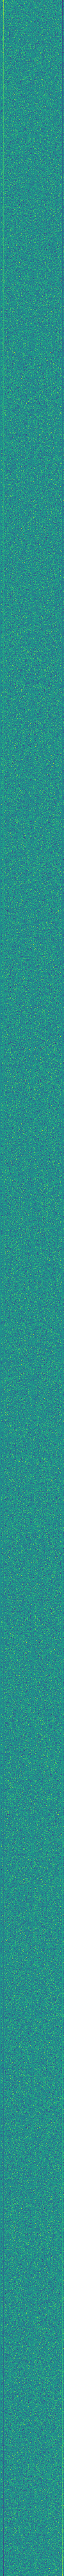
\includegraphics[interpolate=false,width=1.000000in,height=1.000000in]{antiderivative_ci_5-img0.png}}%
\end{pgfscope}%
\begin{pgfscope}%
\pgfsetbuttcap%
\pgfsetroundjoin%
\definecolor{currentfill}{rgb}{0.000000,0.000000,0.000000}%
\pgfsetfillcolor{currentfill}%
\pgfsetlinewidth{0.803000pt}%
\definecolor{currentstroke}{rgb}{0.000000,0.000000,0.000000}%
\pgfsetstrokecolor{currentstroke}%
\pgfsetdash{}{0pt}%
\pgfsys@defobject{currentmarker}{\pgfqpoint{0.000000in}{-0.048611in}}{\pgfqpoint{0.000000in}{0.000000in}}{%
\pgfpathmoveto{\pgfqpoint{0.000000in}{0.000000in}}%
\pgfpathlineto{\pgfqpoint{0.000000in}{-0.048611in}}%
\pgfusepath{stroke,fill}%
}%
\begin{pgfscope}%
\pgfsys@transformshift{0.779897in}{0.517039in}%
\pgfsys@useobject{currentmarker}{}%
\end{pgfscope}%
\end{pgfscope}%
\begin{pgfscope}%
\definecolor{textcolor}{rgb}{0.000000,0.000000,0.000000}%
\pgfsetstrokecolor{textcolor}%
\pgfsetfillcolor{textcolor}%
\pgftext[x=0.779897in,y=0.419816in,,top]{\color{textcolor}{\rmfamily\fontsize{12.000000}{14.400000}\selectfont\catcode`\^=\active\def^{\ifmmode\sp\else\^{}\fi}\catcode`\%=\active\def%{\%}0}}%
\end{pgfscope}%
\begin{pgfscope}%
\pgfsetbuttcap%
\pgfsetroundjoin%
\definecolor{currentfill}{rgb}{0.000000,0.000000,0.000000}%
\pgfsetfillcolor{currentfill}%
\pgfsetlinewidth{0.803000pt}%
\definecolor{currentstroke}{rgb}{0.000000,0.000000,0.000000}%
\pgfsetstrokecolor{currentstroke}%
\pgfsetdash{}{0pt}%
\pgfsys@defobject{currentmarker}{\pgfqpoint{0.000000in}{-0.048611in}}{\pgfqpoint{0.000000in}{0.000000in}}{%
\pgfpathmoveto{\pgfqpoint{0.000000in}{0.000000in}}%
\pgfpathlineto{\pgfqpoint{0.000000in}{-0.048611in}}%
\pgfusepath{stroke,fill}%
}%
\begin{pgfscope}%
\pgfsys@transformshift{1.693017in}{0.517039in}%
\pgfsys@useobject{currentmarker}{}%
\end{pgfscope}%
\end{pgfscope}%
\begin{pgfscope}%
\definecolor{textcolor}{rgb}{0.000000,0.000000,0.000000}%
\pgfsetstrokecolor{textcolor}%
\pgfsetfillcolor{textcolor}%
\pgftext[x=1.693017in,y=0.419816in,,top]{\color{textcolor}{\rmfamily\fontsize{12.000000}{14.400000}\selectfont\catcode`\^=\active\def^{\ifmmode\sp\else\^{}\fi}\catcode`\%=\active\def%{\%}20}}%
\end{pgfscope}%
\begin{pgfscope}%
\pgfsetbuttcap%
\pgfsetroundjoin%
\definecolor{currentfill}{rgb}{0.000000,0.000000,0.000000}%
\pgfsetfillcolor{currentfill}%
\pgfsetlinewidth{0.803000pt}%
\definecolor{currentstroke}{rgb}{0.000000,0.000000,0.000000}%
\pgfsetstrokecolor{currentstroke}%
\pgfsetdash{}{0pt}%
\pgfsys@defobject{currentmarker}{\pgfqpoint{0.000000in}{-0.048611in}}{\pgfqpoint{0.000000in}{0.000000in}}{%
\pgfpathmoveto{\pgfqpoint{0.000000in}{0.000000in}}%
\pgfpathlineto{\pgfqpoint{0.000000in}{-0.048611in}}%
\pgfusepath{stroke,fill}%
}%
\begin{pgfscope}%
\pgfsys@transformshift{2.606137in}{0.517039in}%
\pgfsys@useobject{currentmarker}{}%
\end{pgfscope}%
\end{pgfscope}%
\begin{pgfscope}%
\definecolor{textcolor}{rgb}{0.000000,0.000000,0.000000}%
\pgfsetstrokecolor{textcolor}%
\pgfsetfillcolor{textcolor}%
\pgftext[x=2.606137in,y=0.419816in,,top]{\color{textcolor}{\rmfamily\fontsize{12.000000}{14.400000}\selectfont\catcode`\^=\active\def^{\ifmmode\sp\else\^{}\fi}\catcode`\%=\active\def%{\%}40}}%
\end{pgfscope}%
\begin{pgfscope}%
\definecolor{textcolor}{rgb}{0.000000,0.000000,0.000000}%
\pgfsetstrokecolor{textcolor}%
\pgfsetfillcolor{textcolor}%
\pgftext[x=1.921297in,y=0.202965in,,top]{\color{textcolor}{\rmfamily\fontsize{12.000000}{14.400000}\selectfont\catcode`\^=\active\def^{\ifmmode\sp\else\^{}\fi}\catcode`\%=\active\def%{\%}input coefficients}}%
\end{pgfscope}%
\begin{pgfscope}%
\pgfsetbuttcap%
\pgfsetroundjoin%
\definecolor{currentfill}{rgb}{0.000000,0.000000,0.000000}%
\pgfsetfillcolor{currentfill}%
\pgfsetlinewidth{0.803000pt}%
\definecolor{currentstroke}{rgb}{0.000000,0.000000,0.000000}%
\pgfsetstrokecolor{currentstroke}%
\pgfsetdash{}{0pt}%
\pgfsys@defobject{currentmarker}{\pgfqpoint{-0.048611in}{0.000000in}}{\pgfqpoint{-0.000000in}{0.000000in}}{%
\pgfpathmoveto{\pgfqpoint{-0.000000in}{0.000000in}}%
\pgfpathlineto{\pgfqpoint{-0.048611in}{0.000000in}}%
\pgfusepath{stroke,fill}%
}%
\begin{pgfscope}%
\pgfsys@transformshift{0.779897in}{2.895016in}%
\pgfsys@useobject{currentmarker}{}%
\end{pgfscope}%
\end{pgfscope}%
\begin{pgfscope}%
\definecolor{textcolor}{rgb}{0.000000,0.000000,0.000000}%
\pgfsetstrokecolor{textcolor}%
\pgfsetfillcolor{textcolor}%
\pgftext[x=0.576636in, y=2.831702in, left, base]{\color{textcolor}{\rmfamily\fontsize{12.000000}{14.400000}\selectfont\catcode`\^=\active\def^{\ifmmode\sp\else\^{}\fi}\catcode`\%=\active\def%{\%}0}}%
\end{pgfscope}%
\begin{pgfscope}%
\pgfsetbuttcap%
\pgfsetroundjoin%
\definecolor{currentfill}{rgb}{0.000000,0.000000,0.000000}%
\pgfsetfillcolor{currentfill}%
\pgfsetlinewidth{0.803000pt}%
\definecolor{currentstroke}{rgb}{0.000000,0.000000,0.000000}%
\pgfsetstrokecolor{currentstroke}%
\pgfsetdash{}{0pt}%
\pgfsys@defobject{currentmarker}{\pgfqpoint{-0.048611in}{0.000000in}}{\pgfqpoint{-0.000000in}{0.000000in}}{%
\pgfpathmoveto{\pgfqpoint{-0.000000in}{0.000000in}}%
\pgfpathlineto{\pgfqpoint{-0.048611in}{0.000000in}}%
\pgfusepath{stroke,fill}%
}%
\begin{pgfscope}%
\pgfsys@transformshift{0.779897in}{2.300522in}%
\pgfsys@useobject{currentmarker}{}%
\end{pgfscope}%
\end{pgfscope}%
\begin{pgfscope}%
\definecolor{textcolor}{rgb}{0.000000,0.000000,0.000000}%
\pgfsetstrokecolor{textcolor}%
\pgfsetfillcolor{textcolor}%
\pgftext[x=0.258521in, y=2.237208in, left, base]{\color{textcolor}{\rmfamily\fontsize{12.000000}{14.400000}\selectfont\catcode`\^=\active\def^{\ifmmode\sp\else\^{}\fi}\catcode`\%=\active\def%{\%}1000}}%
\end{pgfscope}%
\begin{pgfscope}%
\pgfsetbuttcap%
\pgfsetroundjoin%
\definecolor{currentfill}{rgb}{0.000000,0.000000,0.000000}%
\pgfsetfillcolor{currentfill}%
\pgfsetlinewidth{0.803000pt}%
\definecolor{currentstroke}{rgb}{0.000000,0.000000,0.000000}%
\pgfsetstrokecolor{currentstroke}%
\pgfsetdash{}{0pt}%
\pgfsys@defobject{currentmarker}{\pgfqpoint{-0.048611in}{0.000000in}}{\pgfqpoint{-0.000000in}{0.000000in}}{%
\pgfpathmoveto{\pgfqpoint{-0.000000in}{0.000000in}}%
\pgfpathlineto{\pgfqpoint{-0.048611in}{0.000000in}}%
\pgfusepath{stroke,fill}%
}%
\begin{pgfscope}%
\pgfsys@transformshift{0.779897in}{1.706027in}%
\pgfsys@useobject{currentmarker}{}%
\end{pgfscope}%
\end{pgfscope}%
\begin{pgfscope}%
\definecolor{textcolor}{rgb}{0.000000,0.000000,0.000000}%
\pgfsetstrokecolor{textcolor}%
\pgfsetfillcolor{textcolor}%
\pgftext[x=0.258521in, y=1.642714in, left, base]{\color{textcolor}{\rmfamily\fontsize{12.000000}{14.400000}\selectfont\catcode`\^=\active\def^{\ifmmode\sp\else\^{}\fi}\catcode`\%=\active\def%{\%}2000}}%
\end{pgfscope}%
\begin{pgfscope}%
\pgfsetbuttcap%
\pgfsetroundjoin%
\definecolor{currentfill}{rgb}{0.000000,0.000000,0.000000}%
\pgfsetfillcolor{currentfill}%
\pgfsetlinewidth{0.803000pt}%
\definecolor{currentstroke}{rgb}{0.000000,0.000000,0.000000}%
\pgfsetstrokecolor{currentstroke}%
\pgfsetdash{}{0pt}%
\pgfsys@defobject{currentmarker}{\pgfqpoint{-0.048611in}{0.000000in}}{\pgfqpoint{-0.000000in}{0.000000in}}{%
\pgfpathmoveto{\pgfqpoint{-0.000000in}{0.000000in}}%
\pgfpathlineto{\pgfqpoint{-0.048611in}{0.000000in}}%
\pgfusepath{stroke,fill}%
}%
\begin{pgfscope}%
\pgfsys@transformshift{0.779897in}{1.111533in}%
\pgfsys@useobject{currentmarker}{}%
\end{pgfscope}%
\end{pgfscope}%
\begin{pgfscope}%
\definecolor{textcolor}{rgb}{0.000000,0.000000,0.000000}%
\pgfsetstrokecolor{textcolor}%
\pgfsetfillcolor{textcolor}%
\pgftext[x=0.258521in, y=1.048219in, left, base]{\color{textcolor}{\rmfamily\fontsize{12.000000}{14.400000}\selectfont\catcode`\^=\active\def^{\ifmmode\sp\else\^{}\fi}\catcode`\%=\active\def%{\%}3000}}%
\end{pgfscope}%
\begin{pgfscope}%
\pgfsetbuttcap%
\pgfsetroundjoin%
\definecolor{currentfill}{rgb}{0.000000,0.000000,0.000000}%
\pgfsetfillcolor{currentfill}%
\pgfsetlinewidth{0.803000pt}%
\definecolor{currentstroke}{rgb}{0.000000,0.000000,0.000000}%
\pgfsetstrokecolor{currentstroke}%
\pgfsetdash{}{0pt}%
\pgfsys@defobject{currentmarker}{\pgfqpoint{-0.048611in}{0.000000in}}{\pgfqpoint{-0.000000in}{0.000000in}}{%
\pgfpathmoveto{\pgfqpoint{-0.000000in}{0.000000in}}%
\pgfpathlineto{\pgfqpoint{-0.048611in}{0.000000in}}%
\pgfusepath{stroke,fill}%
}%
\begin{pgfscope}%
\pgfsys@transformshift{0.779897in}{0.517039in}%
\pgfsys@useobject{currentmarker}{}%
\end{pgfscope}%
\end{pgfscope}%
\begin{pgfscope}%
\definecolor{textcolor}{rgb}{0.000000,0.000000,0.000000}%
\pgfsetstrokecolor{textcolor}%
\pgfsetfillcolor{textcolor}%
\pgftext[x=0.258521in, y=0.453725in, left, base]{\color{textcolor}{\rmfamily\fontsize{12.000000}{14.400000}\selectfont\catcode`\^=\active\def^{\ifmmode\sp\else\^{}\fi}\catcode`\%=\active\def%{\%}4000}}%
\end{pgfscope}%
\begin{pgfscope}%
\definecolor{textcolor}{rgb}{0.000000,0.000000,0.000000}%
\pgfsetstrokecolor{textcolor}%
\pgfsetfillcolor{textcolor}%
\pgftext[x=0.202965in,y=1.706027in,,bottom,rotate=90.000000]{\color{textcolor}{\rmfamily\fontsize{12.000000}{14.400000}\selectfont\catcode`\^=\active\def^{\ifmmode\sp\else\^{}\fi}\catcode`\%=\active\def%{\%}samples}}%
\end{pgfscope}%
\begin{pgfscope}%
\pgfsetrectcap%
\pgfsetmiterjoin%
\pgfsetlinewidth{0.803000pt}%
\definecolor{currentstroke}{rgb}{0.000000,0.000000,0.000000}%
\pgfsetstrokecolor{currentstroke}%
\pgfsetdash{}{0pt}%
\pgfpathmoveto{\pgfqpoint{0.779897in}{0.517039in}}%
\pgfpathlineto{\pgfqpoint{0.779897in}{2.895016in}}%
\pgfusepath{stroke}%
\end{pgfscope}%
\begin{pgfscope}%
\pgfsetrectcap%
\pgfsetmiterjoin%
\pgfsetlinewidth{0.803000pt}%
\definecolor{currentstroke}{rgb}{0.000000,0.000000,0.000000}%
\pgfsetstrokecolor{currentstroke}%
\pgfsetdash{}{0pt}%
\pgfpathmoveto{\pgfqpoint{3.062697in}{0.517039in}}%
\pgfpathlineto{\pgfqpoint{3.062697in}{2.895016in}}%
\pgfusepath{stroke}%
\end{pgfscope}%
\begin{pgfscope}%
\pgfsetrectcap%
\pgfsetmiterjoin%
\pgfsetlinewidth{0.803000pt}%
\definecolor{currentstroke}{rgb}{0.000000,0.000000,0.000000}%
\pgfsetstrokecolor{currentstroke}%
\pgfsetdash{}{0pt}%
\pgfpathmoveto{\pgfqpoint{0.779897in}{0.517039in}}%
\pgfpathlineto{\pgfqpoint{3.062697in}{0.517039in}}%
\pgfusepath{stroke}%
\end{pgfscope}%
\begin{pgfscope}%
\pgfsetrectcap%
\pgfsetmiterjoin%
\pgfsetlinewidth{0.803000pt}%
\definecolor{currentstroke}{rgb}{0.000000,0.000000,0.000000}%
\pgfsetstrokecolor{currentstroke}%
\pgfsetdash{}{0pt}%
\pgfpathmoveto{\pgfqpoint{0.779897in}{2.895016in}}%
\pgfpathlineto{\pgfqpoint{3.062697in}{2.895016in}}%
\pgfusepath{stroke}%
\end{pgfscope}%
\begin{pgfscope}%
\pgfsetbuttcap%
\pgfsetmiterjoin%
\pgfsetlinewidth{0.000000pt}%
\definecolor{currentstroke}{rgb}{0.000000,0.000000,0.000000}%
\pgfsetstrokecolor{currentstroke}%
\pgfsetstrokeopacity{0.000000}%
\pgfsetdash{}{0pt}%
\pgfpathmoveto{\pgfqpoint{3.282875in}{0.517039in}}%
\pgfpathlineto{\pgfqpoint{3.401774in}{0.517039in}}%
\pgfpathlineto{\pgfqpoint{3.401774in}{2.895016in}}%
\pgfpathlineto{\pgfqpoint{3.282875in}{2.895016in}}%
\pgfpathlineto{\pgfqpoint{3.282875in}{0.517039in}}%
\pgfpathclose%
\pgfusepath{}%
\end{pgfscope}%
\begin{pgfscope}%
\pgfsys@transformshift{3.280000in}{0.520000in}%
\pgftext[left,bottom]{
\includegraphics[interpolate=true,width=0.120000in,height=2.380000in]{antiderivative_ci_5-img1.png}}%
\end{pgfscope}%
\begin{pgfscope}%
\pgfsetbuttcap%
\pgfsetroundjoin%
\definecolor{currentfill}{rgb}{0.000000,0.000000,0.000000}%
\pgfsetfillcolor{currentfill}%
\pgfsetlinewidth{0.803000pt}%
\definecolor{currentstroke}{rgb}{0.000000,0.000000,0.000000}%
\pgfsetstrokecolor{currentstroke}%
\pgfsetdash{}{0pt}%
\pgfsys@defobject{currentmarker}{\pgfqpoint{0.000000in}{0.000000in}}{\pgfqpoint{0.048611in}{0.000000in}}{%
\pgfpathmoveto{\pgfqpoint{0.000000in}{0.000000in}}%
\pgfpathlineto{\pgfqpoint{0.048611in}{0.000000in}}%
\pgfusepath{stroke,fill}%
}%
\begin{pgfscope}%
\pgfsys@transformshift{3.401774in}{0.636505in}%
\pgfsys@useobject{currentmarker}{}%
\end{pgfscope}%
\end{pgfscope}%
\begin{pgfscope}%
\definecolor{textcolor}{rgb}{0.000000,0.000000,0.000000}%
\pgfsetstrokecolor{textcolor}%
\pgfsetfillcolor{textcolor}%
\pgftext[x=3.498996in, y=0.573191in, left, base]{\color{textcolor}{\rmfamily\fontsize{12.000000}{14.400000}\selectfont\catcode`\^=\active\def^{\ifmmode\sp\else\^{}\fi}\catcode`\%=\active\def%{\%}\ensuremath{-}100}}%
\end{pgfscope}%
\begin{pgfscope}%
\pgfsetbuttcap%
\pgfsetroundjoin%
\definecolor{currentfill}{rgb}{0.000000,0.000000,0.000000}%
\pgfsetfillcolor{currentfill}%
\pgfsetlinewidth{0.803000pt}%
\definecolor{currentstroke}{rgb}{0.000000,0.000000,0.000000}%
\pgfsetstrokecolor{currentstroke}%
\pgfsetdash{}{0pt}%
\pgfsys@defobject{currentmarker}{\pgfqpoint{0.000000in}{0.000000in}}{\pgfqpoint{0.048611in}{0.000000in}}{%
\pgfpathmoveto{\pgfqpoint{0.000000in}{0.000000in}}%
\pgfpathlineto{\pgfqpoint{0.048611in}{0.000000in}}%
\pgfusepath{stroke,fill}%
}%
\begin{pgfscope}%
\pgfsys@transformshift{3.401774in}{1.171266in}%
\pgfsys@useobject{currentmarker}{}%
\end{pgfscope}%
\end{pgfscope}%
\begin{pgfscope}%
\definecolor{textcolor}{rgb}{0.000000,0.000000,0.000000}%
\pgfsetstrokecolor{textcolor}%
\pgfsetfillcolor{textcolor}%
\pgftext[x=3.498996in, y=1.107952in, left, base]{\color{textcolor}{\rmfamily\fontsize{12.000000}{14.400000}\selectfont\catcode`\^=\active\def^{\ifmmode\sp\else\^{}\fi}\catcode`\%=\active\def%{\%}\ensuremath{-}50}}%
\end{pgfscope}%
\begin{pgfscope}%
\pgfsetbuttcap%
\pgfsetroundjoin%
\definecolor{currentfill}{rgb}{0.000000,0.000000,0.000000}%
\pgfsetfillcolor{currentfill}%
\pgfsetlinewidth{0.803000pt}%
\definecolor{currentstroke}{rgb}{0.000000,0.000000,0.000000}%
\pgfsetstrokecolor{currentstroke}%
\pgfsetdash{}{0pt}%
\pgfsys@defobject{currentmarker}{\pgfqpoint{0.000000in}{0.000000in}}{\pgfqpoint{0.048611in}{0.000000in}}{%
\pgfpathmoveto{\pgfqpoint{0.000000in}{0.000000in}}%
\pgfpathlineto{\pgfqpoint{0.048611in}{0.000000in}}%
\pgfusepath{stroke,fill}%
}%
\begin{pgfscope}%
\pgfsys@transformshift{3.401774in}{1.706028in}%
\pgfsys@useobject{currentmarker}{}%
\end{pgfscope}%
\end{pgfscope}%
\begin{pgfscope}%
\definecolor{textcolor}{rgb}{0.000000,0.000000,0.000000}%
\pgfsetstrokecolor{textcolor}%
\pgfsetfillcolor{textcolor}%
\pgftext[x=3.498996in, y=1.642714in, left, base]{\color{textcolor}{\rmfamily\fontsize{12.000000}{14.400000}\selectfont\catcode`\^=\active\def^{\ifmmode\sp\else\^{}\fi}\catcode`\%=\active\def%{\%}0}}%
\end{pgfscope}%
\begin{pgfscope}%
\pgfsetbuttcap%
\pgfsetroundjoin%
\definecolor{currentfill}{rgb}{0.000000,0.000000,0.000000}%
\pgfsetfillcolor{currentfill}%
\pgfsetlinewidth{0.803000pt}%
\definecolor{currentstroke}{rgb}{0.000000,0.000000,0.000000}%
\pgfsetstrokecolor{currentstroke}%
\pgfsetdash{}{0pt}%
\pgfsys@defobject{currentmarker}{\pgfqpoint{0.000000in}{0.000000in}}{\pgfqpoint{0.048611in}{0.000000in}}{%
\pgfpathmoveto{\pgfqpoint{0.000000in}{0.000000in}}%
\pgfpathlineto{\pgfqpoint{0.048611in}{0.000000in}}%
\pgfusepath{stroke,fill}%
}%
\begin{pgfscope}%
\pgfsys@transformshift{3.401774in}{2.240789in}%
\pgfsys@useobject{currentmarker}{}%
\end{pgfscope}%
\end{pgfscope}%
\begin{pgfscope}%
\definecolor{textcolor}{rgb}{0.000000,0.000000,0.000000}%
\pgfsetstrokecolor{textcolor}%
\pgfsetfillcolor{textcolor}%
\pgftext[x=3.498996in, y=2.177475in, left, base]{\color{textcolor}{\rmfamily\fontsize{12.000000}{14.400000}\selectfont\catcode`\^=\active\def^{\ifmmode\sp\else\^{}\fi}\catcode`\%=\active\def%{\%}50}}%
\end{pgfscope}%
\begin{pgfscope}%
\pgfsetbuttcap%
\pgfsetroundjoin%
\definecolor{currentfill}{rgb}{0.000000,0.000000,0.000000}%
\pgfsetfillcolor{currentfill}%
\pgfsetlinewidth{0.803000pt}%
\definecolor{currentstroke}{rgb}{0.000000,0.000000,0.000000}%
\pgfsetstrokecolor{currentstroke}%
\pgfsetdash{}{0pt}%
\pgfsys@defobject{currentmarker}{\pgfqpoint{0.000000in}{0.000000in}}{\pgfqpoint{0.048611in}{0.000000in}}{%
\pgfpathmoveto{\pgfqpoint{0.000000in}{0.000000in}}%
\pgfpathlineto{\pgfqpoint{0.048611in}{0.000000in}}%
\pgfusepath{stroke,fill}%
}%
\begin{pgfscope}%
\pgfsys@transformshift{3.401774in}{2.775550in}%
\pgfsys@useobject{currentmarker}{}%
\end{pgfscope}%
\end{pgfscope}%
\begin{pgfscope}%
\definecolor{textcolor}{rgb}{0.000000,0.000000,0.000000}%
\pgfsetstrokecolor{textcolor}%
\pgfsetfillcolor{textcolor}%
\pgftext[x=3.498996in, y=2.712237in, left, base]{\color{textcolor}{\rmfamily\fontsize{12.000000}{14.400000}\selectfont\catcode`\^=\active\def^{\ifmmode\sp\else\^{}\fi}\catcode`\%=\active\def%{\%}100}}%
\end{pgfscope}%
\begin{pgfscope}%
\pgfsetrectcap%
\pgfsetmiterjoin%
\pgfsetlinewidth{0.803000pt}%
\definecolor{currentstroke}{rgb}{0.000000,0.000000,0.000000}%
\pgfsetstrokecolor{currentstroke}%
\pgfsetdash{}{0pt}%
\pgfpathmoveto{\pgfqpoint{3.282875in}{0.517039in}}%
\pgfpathlineto{\pgfqpoint{3.342325in}{0.517039in}}%
\pgfpathlineto{\pgfqpoint{3.401774in}{0.517039in}}%
\pgfpathlineto{\pgfqpoint{3.401774in}{2.895016in}}%
\pgfpathlineto{\pgfqpoint{3.342325in}{2.895016in}}%
\pgfpathlineto{\pgfqpoint{3.282875in}{2.895016in}}%
\pgfpathlineto{\pgfqpoint{3.282875in}{0.517039in}}%
\pgfpathclose%
\pgfusepath{stroke}%
\end{pgfscope}%
\end{pgfpicture}%
\makeatother%
\endgroup%

    \end{adjustbox}
    \caption{Correlation image 5\% noise.}\label{fig:sc1_ci_5}
  \end{subfigure}
  \begin{subfigure}{0.49\linewidth}
    \begin{adjustbox}{width=1.2\linewidth}
      \begingroup%
\makeatletter%
\begin{pgfpicture}%
\pgfpathrectangle{\pgfpointorigin}{\pgfqpoint{6.400000in}{4.800000in}}%
\pgfusepath{use as bounding box, clip}%
\begin{pgfscope}%
\pgfsetbuttcap%
\pgfsetmiterjoin%
\pgfsetlinewidth{0.000000pt}%
\definecolor{currentstroke}{rgb}{0.000000,0.000000,0.000000}%
\pgfsetstrokecolor{currentstroke}%
\pgfsetstrokeopacity{0.000000}%
\pgfsetdash{}{0pt}%
\pgfpathmoveto{\pgfqpoint{0.000000in}{0.000000in}}%
\pgfpathlineto{\pgfqpoint{6.400000in}{0.000000in}}%
\pgfpathlineto{\pgfqpoint{6.400000in}{4.800000in}}%
\pgfpathlineto{\pgfqpoint{0.000000in}{4.800000in}}%
\pgfpathlineto{\pgfqpoint{0.000000in}{0.000000in}}%
\pgfpathclose%
\pgfusepath{}%
\end{pgfscope}%
\begin{pgfscope}%
\pgfsetbuttcap%
\pgfsetmiterjoin%
\pgfsetlinewidth{0.000000pt}%
\definecolor{currentstroke}{rgb}{0.000000,0.000000,0.000000}%
\pgfsetstrokecolor{currentstroke}%
\pgfsetstrokeopacity{0.000000}%
\pgfsetdash{}{0pt}%
\pgfpathmoveto{\pgfqpoint{1.072000in}{0.528000in}}%
\pgfpathlineto{\pgfqpoint{4.768000in}{0.528000in}}%
\pgfpathlineto{\pgfqpoint{4.768000in}{4.224000in}}%
\pgfpathlineto{\pgfqpoint{1.072000in}{4.224000in}}%
\pgfpathlineto{\pgfqpoint{1.072000in}{0.528000in}}%
\pgfpathclose%
\pgfusepath{}%
\end{pgfscope}%
\begin{pgfscope}%
\pgfpathrectangle{\pgfqpoint{1.072000in}{0.528000in}}{\pgfqpoint{3.696000in}{3.696000in}}%
\pgfusepath{clip}%
\pgfsys@transformcm{3.696000}{0.000000}{0.000000}{-3.696000}{1.072000in}{4.224000in}%
\pgftext[left,bottom]{
\includegraphics[interpolate=false,width=1.000000in,height=1.000000in]{antiderivative_pm_5-img0.png}}%
\end{pgfscope}%
\begin{pgfscope}%
\pgfsetbuttcap%
\pgfsetroundjoin%
\definecolor{currentfill}{rgb}{0.000000,0.000000,0.000000}%
\pgfsetfillcolor{currentfill}%
\pgfsetlinewidth{0.803000pt}%
\definecolor{currentstroke}{rgb}{0.000000,0.000000,0.000000}%
\pgfsetstrokecolor{currentstroke}%
\pgfsetdash{}{0pt}%
\pgfsys@defobject{currentmarker}{\pgfqpoint{0.000000in}{-0.048611in}}{\pgfqpoint{0.000000in}{0.000000in}}{%
\pgfpathmoveto{\pgfqpoint{0.000000in}{0.000000in}}%
\pgfpathlineto{\pgfqpoint{0.000000in}{-0.048611in}}%
\pgfusepath{stroke,fill}%
}%
\begin{pgfscope}%
\pgfsys@transformshift{1.090480in}{0.528000in}%
\pgfsys@useobject{currentmarker}{}%
\end{pgfscope}%
\end{pgfscope}%
\begin{pgfscope}%
\definecolor{textcolor}{rgb}{0.000000,0.000000,0.000000}%
\pgfsetstrokecolor{textcolor}%
\pgfsetfillcolor{textcolor}%
\pgftext[x=1.090480in,y=0.430778in,,top]{\color{textcolor}{\rmfamily\fontsize{12.000000}{14.400000}\selectfont\catcode`\^=\active\def^{\ifmmode\sp\else\^{}\fi}\catcode`\%=\active\def%{\%}0}}%
\end{pgfscope}%
\begin{pgfscope}%
\pgfsetbuttcap%
\pgfsetroundjoin%
\definecolor{currentfill}{rgb}{0.000000,0.000000,0.000000}%
\pgfsetfillcolor{currentfill}%
\pgfsetlinewidth{0.803000pt}%
\definecolor{currentstroke}{rgb}{0.000000,0.000000,0.000000}%
\pgfsetstrokecolor{currentstroke}%
\pgfsetdash{}{0pt}%
\pgfsys@defobject{currentmarker}{\pgfqpoint{0.000000in}{-0.048611in}}{\pgfqpoint{0.000000in}{0.000000in}}{%
\pgfpathmoveto{\pgfqpoint{0.000000in}{0.000000in}}%
\pgfpathlineto{\pgfqpoint{0.000000in}{-0.048611in}}%
\pgfusepath{stroke,fill}%
}%
\begin{pgfscope}%
\pgfsys@transformshift{1.829680in}{0.528000in}%
\pgfsys@useobject{currentmarker}{}%
\end{pgfscope}%
\end{pgfscope}%
\begin{pgfscope}%
\definecolor{textcolor}{rgb}{0.000000,0.000000,0.000000}%
\pgfsetstrokecolor{textcolor}%
\pgfsetfillcolor{textcolor}%
\pgftext[x=1.829680in,y=0.430778in,,top]{\color{textcolor}{\rmfamily\fontsize{12.000000}{14.400000}\selectfont\catcode`\^=\active\def^{\ifmmode\sp\else\^{}\fi}\catcode`\%=\active\def%{\%}20}}%
\end{pgfscope}%
\begin{pgfscope}%
\pgfsetbuttcap%
\pgfsetroundjoin%
\definecolor{currentfill}{rgb}{0.000000,0.000000,0.000000}%
\pgfsetfillcolor{currentfill}%
\pgfsetlinewidth{0.803000pt}%
\definecolor{currentstroke}{rgb}{0.000000,0.000000,0.000000}%
\pgfsetstrokecolor{currentstroke}%
\pgfsetdash{}{0pt}%
\pgfsys@defobject{currentmarker}{\pgfqpoint{0.000000in}{-0.048611in}}{\pgfqpoint{0.000000in}{0.000000in}}{%
\pgfpathmoveto{\pgfqpoint{0.000000in}{0.000000in}}%
\pgfpathlineto{\pgfqpoint{0.000000in}{-0.048611in}}%
\pgfusepath{stroke,fill}%
}%
\begin{pgfscope}%
\pgfsys@transformshift{2.568880in}{0.528000in}%
\pgfsys@useobject{currentmarker}{}%
\end{pgfscope}%
\end{pgfscope}%
\begin{pgfscope}%
\definecolor{textcolor}{rgb}{0.000000,0.000000,0.000000}%
\pgfsetstrokecolor{textcolor}%
\pgfsetfillcolor{textcolor}%
\pgftext[x=2.568880in,y=0.430778in,,top]{\color{textcolor}{\rmfamily\fontsize{12.000000}{14.400000}\selectfont\catcode`\^=\active\def^{\ifmmode\sp\else\^{}\fi}\catcode`\%=\active\def%{\%}40}}%
\end{pgfscope}%
\begin{pgfscope}%
\pgfsetbuttcap%
\pgfsetroundjoin%
\definecolor{currentfill}{rgb}{0.000000,0.000000,0.000000}%
\pgfsetfillcolor{currentfill}%
\pgfsetlinewidth{0.803000pt}%
\definecolor{currentstroke}{rgb}{0.000000,0.000000,0.000000}%
\pgfsetstrokecolor{currentstroke}%
\pgfsetdash{}{0pt}%
\pgfsys@defobject{currentmarker}{\pgfqpoint{0.000000in}{-0.048611in}}{\pgfqpoint{0.000000in}{0.000000in}}{%
\pgfpathmoveto{\pgfqpoint{0.000000in}{0.000000in}}%
\pgfpathlineto{\pgfqpoint{0.000000in}{-0.048611in}}%
\pgfusepath{stroke,fill}%
}%
\begin{pgfscope}%
\pgfsys@transformshift{3.308080in}{0.528000in}%
\pgfsys@useobject{currentmarker}{}%
\end{pgfscope}%
\end{pgfscope}%
\begin{pgfscope}%
\definecolor{textcolor}{rgb}{0.000000,0.000000,0.000000}%
\pgfsetstrokecolor{textcolor}%
\pgfsetfillcolor{textcolor}%
\pgftext[x=3.308080in,y=0.430778in,,top]{\color{textcolor}{\rmfamily\fontsize{12.000000}{14.400000}\selectfont\catcode`\^=\active\def^{\ifmmode\sp\else\^{}\fi}\catcode`\%=\active\def%{\%}60}}%
\end{pgfscope}%
\begin{pgfscope}%
\pgfsetbuttcap%
\pgfsetroundjoin%
\definecolor{currentfill}{rgb}{0.000000,0.000000,0.000000}%
\pgfsetfillcolor{currentfill}%
\pgfsetlinewidth{0.803000pt}%
\definecolor{currentstroke}{rgb}{0.000000,0.000000,0.000000}%
\pgfsetstrokecolor{currentstroke}%
\pgfsetdash{}{0pt}%
\pgfsys@defobject{currentmarker}{\pgfqpoint{0.000000in}{-0.048611in}}{\pgfqpoint{0.000000in}{0.000000in}}{%
\pgfpathmoveto{\pgfqpoint{0.000000in}{0.000000in}}%
\pgfpathlineto{\pgfqpoint{0.000000in}{-0.048611in}}%
\pgfusepath{stroke,fill}%
}%
\begin{pgfscope}%
\pgfsys@transformshift{4.047280in}{0.528000in}%
\pgfsys@useobject{currentmarker}{}%
\end{pgfscope}%
\end{pgfscope}%
\begin{pgfscope}%
\definecolor{textcolor}{rgb}{0.000000,0.000000,0.000000}%
\pgfsetstrokecolor{textcolor}%
\pgfsetfillcolor{textcolor}%
\pgftext[x=4.047280in,y=0.430778in,,top]{\color{textcolor}{\rmfamily\fontsize{12.000000}{14.400000}\selectfont\catcode`\^=\active\def^{\ifmmode\sp\else\^{}\fi}\catcode`\%=\active\def%{\%}80}}%
\end{pgfscope}%
\begin{pgfscope}%
\definecolor{textcolor}{rgb}{0.000000,0.000000,0.000000}%
\pgfsetstrokecolor{textcolor}%
\pgfsetfillcolor{textcolor}%
\pgftext[x=2.920000in,y=0.213927in,,top]{\color{textcolor}{\rmfamily\fontsize{12.000000}{14.400000}\selectfont\catcode`\^=\active\def^{\ifmmode\sp\else\^{}\fi}\catcode`\%=\active\def%{\%}output coefficients}}%
\end{pgfscope}%
\begin{pgfscope}%
\pgfsetbuttcap%
\pgfsetroundjoin%
\definecolor{currentfill}{rgb}{0.000000,0.000000,0.000000}%
\pgfsetfillcolor{currentfill}%
\pgfsetlinewidth{0.803000pt}%
\definecolor{currentstroke}{rgb}{0.000000,0.000000,0.000000}%
\pgfsetstrokecolor{currentstroke}%
\pgfsetdash{}{0pt}%
\pgfsys@defobject{currentmarker}{\pgfqpoint{-0.048611in}{0.000000in}}{\pgfqpoint{-0.000000in}{0.000000in}}{%
\pgfpathmoveto{\pgfqpoint{-0.000000in}{0.000000in}}%
\pgfpathlineto{\pgfqpoint{-0.048611in}{0.000000in}}%
\pgfusepath{stroke,fill}%
}%
\begin{pgfscope}%
\pgfsys@transformshift{1.072000in}{4.205520in}%
\pgfsys@useobject{currentmarker}{}%
\end{pgfscope}%
\end{pgfscope}%
\begin{pgfscope}%
\definecolor{textcolor}{rgb}{0.000000,0.000000,0.000000}%
\pgfsetstrokecolor{textcolor}%
\pgfsetfillcolor{textcolor}%
\pgftext[x=0.868739in, y=4.142206in, left, base]{\color{textcolor}{\rmfamily\fontsize{12.000000}{14.400000}\selectfont\catcode`\^=\active\def^{\ifmmode\sp\else\^{}\fi}\catcode`\%=\active\def%{\%}0}}%
\end{pgfscope}%
\begin{pgfscope}%
\pgfsetbuttcap%
\pgfsetroundjoin%
\definecolor{currentfill}{rgb}{0.000000,0.000000,0.000000}%
\pgfsetfillcolor{currentfill}%
\pgfsetlinewidth{0.803000pt}%
\definecolor{currentstroke}{rgb}{0.000000,0.000000,0.000000}%
\pgfsetstrokecolor{currentstroke}%
\pgfsetdash{}{0pt}%
\pgfsys@defobject{currentmarker}{\pgfqpoint{-0.048611in}{0.000000in}}{\pgfqpoint{-0.000000in}{0.000000in}}{%
\pgfpathmoveto{\pgfqpoint{-0.000000in}{0.000000in}}%
\pgfpathlineto{\pgfqpoint{-0.048611in}{0.000000in}}%
\pgfusepath{stroke,fill}%
}%
\begin{pgfscope}%
\pgfsys@transformshift{1.072000in}{3.466320in}%
\pgfsys@useobject{currentmarker}{}%
\end{pgfscope}%
\end{pgfscope}%
\begin{pgfscope}%
\definecolor{textcolor}{rgb}{0.000000,0.000000,0.000000}%
\pgfsetstrokecolor{textcolor}%
\pgfsetfillcolor{textcolor}%
\pgftext[x=0.762701in, y=3.403006in, left, base]{\color{textcolor}{\rmfamily\fontsize{12.000000}{14.400000}\selectfont\catcode`\^=\active\def^{\ifmmode\sp\else\^{}\fi}\catcode`\%=\active\def%{\%}20}}%
\end{pgfscope}%
\begin{pgfscope}%
\pgfsetbuttcap%
\pgfsetroundjoin%
\definecolor{currentfill}{rgb}{0.000000,0.000000,0.000000}%
\pgfsetfillcolor{currentfill}%
\pgfsetlinewidth{0.803000pt}%
\definecolor{currentstroke}{rgb}{0.000000,0.000000,0.000000}%
\pgfsetstrokecolor{currentstroke}%
\pgfsetdash{}{0pt}%
\pgfsys@defobject{currentmarker}{\pgfqpoint{-0.048611in}{0.000000in}}{\pgfqpoint{-0.000000in}{0.000000in}}{%
\pgfpathmoveto{\pgfqpoint{-0.000000in}{0.000000in}}%
\pgfpathlineto{\pgfqpoint{-0.048611in}{0.000000in}}%
\pgfusepath{stroke,fill}%
}%
\begin{pgfscope}%
\pgfsys@transformshift{1.072000in}{2.727120in}%
\pgfsys@useobject{currentmarker}{}%
\end{pgfscope}%
\end{pgfscope}%
\begin{pgfscope}%
\definecolor{textcolor}{rgb}{0.000000,0.000000,0.000000}%
\pgfsetstrokecolor{textcolor}%
\pgfsetfillcolor{textcolor}%
\pgftext[x=0.762701in, y=2.663806in, left, base]{\color{textcolor}{\rmfamily\fontsize{12.000000}{14.400000}\selectfont\catcode`\^=\active\def^{\ifmmode\sp\else\^{}\fi}\catcode`\%=\active\def%{\%}40}}%
\end{pgfscope}%
\begin{pgfscope}%
\pgfsetbuttcap%
\pgfsetroundjoin%
\definecolor{currentfill}{rgb}{0.000000,0.000000,0.000000}%
\pgfsetfillcolor{currentfill}%
\pgfsetlinewidth{0.803000pt}%
\definecolor{currentstroke}{rgb}{0.000000,0.000000,0.000000}%
\pgfsetstrokecolor{currentstroke}%
\pgfsetdash{}{0pt}%
\pgfsys@defobject{currentmarker}{\pgfqpoint{-0.048611in}{0.000000in}}{\pgfqpoint{-0.000000in}{0.000000in}}{%
\pgfpathmoveto{\pgfqpoint{-0.000000in}{0.000000in}}%
\pgfpathlineto{\pgfqpoint{-0.048611in}{0.000000in}}%
\pgfusepath{stroke,fill}%
}%
\begin{pgfscope}%
\pgfsys@transformshift{1.072000in}{1.987920in}%
\pgfsys@useobject{currentmarker}{}%
\end{pgfscope}%
\end{pgfscope}%
\begin{pgfscope}%
\definecolor{textcolor}{rgb}{0.000000,0.000000,0.000000}%
\pgfsetstrokecolor{textcolor}%
\pgfsetfillcolor{textcolor}%
\pgftext[x=0.762701in, y=1.924606in, left, base]{\color{textcolor}{\rmfamily\fontsize{12.000000}{14.400000}\selectfont\catcode`\^=\active\def^{\ifmmode\sp\else\^{}\fi}\catcode`\%=\active\def%{\%}60}}%
\end{pgfscope}%
\begin{pgfscope}%
\pgfsetbuttcap%
\pgfsetroundjoin%
\definecolor{currentfill}{rgb}{0.000000,0.000000,0.000000}%
\pgfsetfillcolor{currentfill}%
\pgfsetlinewidth{0.803000pt}%
\definecolor{currentstroke}{rgb}{0.000000,0.000000,0.000000}%
\pgfsetstrokecolor{currentstroke}%
\pgfsetdash{}{0pt}%
\pgfsys@defobject{currentmarker}{\pgfqpoint{-0.048611in}{0.000000in}}{\pgfqpoint{-0.000000in}{0.000000in}}{%
\pgfpathmoveto{\pgfqpoint{-0.000000in}{0.000000in}}%
\pgfpathlineto{\pgfqpoint{-0.048611in}{0.000000in}}%
\pgfusepath{stroke,fill}%
}%
\begin{pgfscope}%
\pgfsys@transformshift{1.072000in}{1.248720in}%
\pgfsys@useobject{currentmarker}{}%
\end{pgfscope}%
\end{pgfscope}%
\begin{pgfscope}%
\definecolor{textcolor}{rgb}{0.000000,0.000000,0.000000}%
\pgfsetstrokecolor{textcolor}%
\pgfsetfillcolor{textcolor}%
\pgftext[x=0.762701in, y=1.185406in, left, base]{\color{textcolor}{\rmfamily\fontsize{12.000000}{14.400000}\selectfont\catcode`\^=\active\def^{\ifmmode\sp\else\^{}\fi}\catcode`\%=\active\def%{\%}80}}%
\end{pgfscope}%
\begin{pgfscope}%
\definecolor{textcolor}{rgb}{0.000000,0.000000,0.000000}%
\pgfsetstrokecolor{textcolor}%
\pgfsetfillcolor{textcolor}%
\pgftext[x=0.707145in,y=2.376000in,,bottom,rotate=90.000000]{\color{textcolor}{\rmfamily\fontsize{12.000000}{14.400000}\selectfont\catcode`\^=\active\def^{\ifmmode\sp\else\^{}\fi}\catcode`\%=\active\def%{\%}input coefficients}}%
\end{pgfscope}%
\begin{pgfscope}%
\pgfsetrectcap%
\pgfsetmiterjoin%
\pgfsetlinewidth{0.803000pt}%
\definecolor{currentstroke}{rgb}{0.000000,0.000000,0.000000}%
\pgfsetstrokecolor{currentstroke}%
\pgfsetdash{}{0pt}%
\pgfpathmoveto{\pgfqpoint{1.072000in}{0.528000in}}%
\pgfpathlineto{\pgfqpoint{1.072000in}{4.224000in}}%
\pgfusepath{stroke}%
\end{pgfscope}%
\begin{pgfscope}%
\pgfsetrectcap%
\pgfsetmiterjoin%
\pgfsetlinewidth{0.803000pt}%
\definecolor{currentstroke}{rgb}{0.000000,0.000000,0.000000}%
\pgfsetstrokecolor{currentstroke}%
\pgfsetdash{}{0pt}%
\pgfpathmoveto{\pgfqpoint{4.768000in}{0.528000in}}%
\pgfpathlineto{\pgfqpoint{4.768000in}{4.224000in}}%
\pgfusepath{stroke}%
\end{pgfscope}%
\begin{pgfscope}%
\pgfsetrectcap%
\pgfsetmiterjoin%
\pgfsetlinewidth{0.803000pt}%
\definecolor{currentstroke}{rgb}{0.000000,0.000000,0.000000}%
\pgfsetstrokecolor{currentstroke}%
\pgfsetdash{}{0pt}%
\pgfpathmoveto{\pgfqpoint{1.072000in}{0.528000in}}%
\pgfpathlineto{\pgfqpoint{4.768000in}{0.528000in}}%
\pgfusepath{stroke}%
\end{pgfscope}%
\begin{pgfscope}%
\pgfsetrectcap%
\pgfsetmiterjoin%
\pgfsetlinewidth{0.803000pt}%
\definecolor{currentstroke}{rgb}{0.000000,0.000000,0.000000}%
\pgfsetstrokecolor{currentstroke}%
\pgfsetdash{}{0pt}%
\pgfpathmoveto{\pgfqpoint{1.072000in}{4.224000in}}%
\pgfpathlineto{\pgfqpoint{4.768000in}{4.224000in}}%
\pgfusepath{stroke}%
\end{pgfscope}%
\begin{pgfscope}%
\pgfsetbuttcap%
\pgfsetmiterjoin%
\pgfsetlinewidth{0.000000pt}%
\definecolor{currentstroke}{rgb}{0.000000,0.000000,0.000000}%
\pgfsetstrokecolor{currentstroke}%
\pgfsetstrokeopacity{0.000000}%
\pgfsetdash{}{0pt}%
\pgfpathmoveto{\pgfqpoint{5.016000in}{0.528000in}}%
\pgfpathlineto{\pgfqpoint{5.200800in}{0.528000in}}%
\pgfpathlineto{\pgfqpoint{5.200800in}{4.224000in}}%
\pgfpathlineto{\pgfqpoint{5.016000in}{4.224000in}}%
\pgfpathlineto{\pgfqpoint{5.016000in}{0.528000in}}%
\pgfpathclose%
\pgfusepath{}%
\end{pgfscope}%
\begin{pgfscope}%
\pgfsys@transformshift{5.020000in}{0.530000in}%
\pgftext[left,bottom]{
\includegraphics[interpolate=true,width=0.180000in,height=3.690000in]{antiderivative_pm_5-img1.png}}%
\end{pgfscope}%
\begin{pgfscope}%
\pgfsetbuttcap%
\pgfsetroundjoin%
\definecolor{currentfill}{rgb}{0.000000,0.000000,0.000000}%
\pgfsetfillcolor{currentfill}%
\pgfsetlinewidth{0.803000pt}%
\definecolor{currentstroke}{rgb}{0.000000,0.000000,0.000000}%
\pgfsetstrokecolor{currentstroke}%
\pgfsetdash{}{0pt}%
\pgfsys@defobject{currentmarker}{\pgfqpoint{0.000000in}{0.000000in}}{\pgfqpoint{0.048611in}{0.000000in}}{%
\pgfpathmoveto{\pgfqpoint{0.000000in}{0.000000in}}%
\pgfpathlineto{\pgfqpoint{0.048611in}{0.000000in}}%
\pgfusepath{stroke,fill}%
}%
\begin{pgfscope}%
\pgfsys@transformshift{5.200800in}{0.806760in}%
\pgfsys@useobject{currentmarker}{}%
\end{pgfscope}%
\end{pgfscope}%
\begin{pgfscope}%
\definecolor{textcolor}{rgb}{0.000000,0.000000,0.000000}%
\pgfsetstrokecolor{textcolor}%
\pgfsetfillcolor{textcolor}%
\pgftext[x=5.298022in, y=0.743447in, left, base]{\color{textcolor}{\rmfamily\fontsize{12.000000}{14.400000}\selectfont\catcode`\^=\active\def^{\ifmmode\sp\else\^{}\fi}\catcode`\%=\active\def%{\%}\ensuremath{-}2000}}%
\end{pgfscope}%
\begin{pgfscope}%
\pgfsetbuttcap%
\pgfsetroundjoin%
\definecolor{currentfill}{rgb}{0.000000,0.000000,0.000000}%
\pgfsetfillcolor{currentfill}%
\pgfsetlinewidth{0.803000pt}%
\definecolor{currentstroke}{rgb}{0.000000,0.000000,0.000000}%
\pgfsetstrokecolor{currentstroke}%
\pgfsetdash{}{0pt}%
\pgfsys@defobject{currentmarker}{\pgfqpoint{0.000000in}{0.000000in}}{\pgfqpoint{0.048611in}{0.000000in}}{%
\pgfpathmoveto{\pgfqpoint{0.000000in}{0.000000in}}%
\pgfpathlineto{\pgfqpoint{0.048611in}{0.000000in}}%
\pgfusepath{stroke,fill}%
}%
\begin{pgfscope}%
\pgfsys@transformshift{5.200800in}{1.404820in}%
\pgfsys@useobject{currentmarker}{}%
\end{pgfscope}%
\end{pgfscope}%
\begin{pgfscope}%
\definecolor{textcolor}{rgb}{0.000000,0.000000,0.000000}%
\pgfsetstrokecolor{textcolor}%
\pgfsetfillcolor{textcolor}%
\pgftext[x=5.298022in, y=1.341506in, left, base]{\color{textcolor}{\rmfamily\fontsize{12.000000}{14.400000}\selectfont\catcode`\^=\active\def^{\ifmmode\sp\else\^{}\fi}\catcode`\%=\active\def%{\%}\ensuremath{-}1500}}%
\end{pgfscope}%
\begin{pgfscope}%
\pgfsetbuttcap%
\pgfsetroundjoin%
\definecolor{currentfill}{rgb}{0.000000,0.000000,0.000000}%
\pgfsetfillcolor{currentfill}%
\pgfsetlinewidth{0.803000pt}%
\definecolor{currentstroke}{rgb}{0.000000,0.000000,0.000000}%
\pgfsetstrokecolor{currentstroke}%
\pgfsetdash{}{0pt}%
\pgfsys@defobject{currentmarker}{\pgfqpoint{0.000000in}{0.000000in}}{\pgfqpoint{0.048611in}{0.000000in}}{%
\pgfpathmoveto{\pgfqpoint{0.000000in}{0.000000in}}%
\pgfpathlineto{\pgfqpoint{0.048611in}{0.000000in}}%
\pgfusepath{stroke,fill}%
}%
\begin{pgfscope}%
\pgfsys@transformshift{5.200800in}{2.002880in}%
\pgfsys@useobject{currentmarker}{}%
\end{pgfscope}%
\end{pgfscope}%
\begin{pgfscope}%
\definecolor{textcolor}{rgb}{0.000000,0.000000,0.000000}%
\pgfsetstrokecolor{textcolor}%
\pgfsetfillcolor{textcolor}%
\pgftext[x=5.298022in, y=1.939566in, left, base]{\color{textcolor}{\rmfamily\fontsize{12.000000}{14.400000}\selectfont\catcode`\^=\active\def^{\ifmmode\sp\else\^{}\fi}\catcode`\%=\active\def%{\%}\ensuremath{-}1000}}%
\end{pgfscope}%
\begin{pgfscope}%
\pgfsetbuttcap%
\pgfsetroundjoin%
\definecolor{currentfill}{rgb}{0.000000,0.000000,0.000000}%
\pgfsetfillcolor{currentfill}%
\pgfsetlinewidth{0.803000pt}%
\definecolor{currentstroke}{rgb}{0.000000,0.000000,0.000000}%
\pgfsetstrokecolor{currentstroke}%
\pgfsetdash{}{0pt}%
\pgfsys@defobject{currentmarker}{\pgfqpoint{0.000000in}{0.000000in}}{\pgfqpoint{0.048611in}{0.000000in}}{%
\pgfpathmoveto{\pgfqpoint{0.000000in}{0.000000in}}%
\pgfpathlineto{\pgfqpoint{0.048611in}{0.000000in}}%
\pgfusepath{stroke,fill}%
}%
\begin{pgfscope}%
\pgfsys@transformshift{5.200800in}{2.600940in}%
\pgfsys@useobject{currentmarker}{}%
\end{pgfscope}%
\end{pgfscope}%
\begin{pgfscope}%
\definecolor{textcolor}{rgb}{0.000000,0.000000,0.000000}%
\pgfsetstrokecolor{textcolor}%
\pgfsetfillcolor{textcolor}%
\pgftext[x=5.298022in, y=2.537626in, left, base]{\color{textcolor}{\rmfamily\fontsize{12.000000}{14.400000}\selectfont\catcode`\^=\active\def^{\ifmmode\sp\else\^{}\fi}\catcode`\%=\active\def%{\%}\ensuremath{-}500}}%
\end{pgfscope}%
\begin{pgfscope}%
\pgfsetbuttcap%
\pgfsetroundjoin%
\definecolor{currentfill}{rgb}{0.000000,0.000000,0.000000}%
\pgfsetfillcolor{currentfill}%
\pgfsetlinewidth{0.803000pt}%
\definecolor{currentstroke}{rgb}{0.000000,0.000000,0.000000}%
\pgfsetstrokecolor{currentstroke}%
\pgfsetdash{}{0pt}%
\pgfsys@defobject{currentmarker}{\pgfqpoint{0.000000in}{0.000000in}}{\pgfqpoint{0.048611in}{0.000000in}}{%
\pgfpathmoveto{\pgfqpoint{0.000000in}{0.000000in}}%
\pgfpathlineto{\pgfqpoint{0.048611in}{0.000000in}}%
\pgfusepath{stroke,fill}%
}%
\begin{pgfscope}%
\pgfsys@transformshift{5.200800in}{3.199000in}%
\pgfsys@useobject{currentmarker}{}%
\end{pgfscope}%
\end{pgfscope}%
\begin{pgfscope}%
\definecolor{textcolor}{rgb}{0.000000,0.000000,0.000000}%
\pgfsetstrokecolor{textcolor}%
\pgfsetfillcolor{textcolor}%
\pgftext[x=5.298022in, y=3.135686in, left, base]{\color{textcolor}{\rmfamily\fontsize{12.000000}{14.400000}\selectfont\catcode`\^=\active\def^{\ifmmode\sp\else\^{}\fi}\catcode`\%=\active\def%{\%}0}}%
\end{pgfscope}%
\begin{pgfscope}%
\pgfsetbuttcap%
\pgfsetroundjoin%
\definecolor{currentfill}{rgb}{0.000000,0.000000,0.000000}%
\pgfsetfillcolor{currentfill}%
\pgfsetlinewidth{0.803000pt}%
\definecolor{currentstroke}{rgb}{0.000000,0.000000,0.000000}%
\pgfsetstrokecolor{currentstroke}%
\pgfsetdash{}{0pt}%
\pgfsys@defobject{currentmarker}{\pgfqpoint{0.000000in}{0.000000in}}{\pgfqpoint{0.048611in}{0.000000in}}{%
\pgfpathmoveto{\pgfqpoint{0.000000in}{0.000000in}}%
\pgfpathlineto{\pgfqpoint{0.048611in}{0.000000in}}%
\pgfusepath{stroke,fill}%
}%
\begin{pgfscope}%
\pgfsys@transformshift{5.200800in}{3.797059in}%
\pgfsys@useobject{currentmarker}{}%
\end{pgfscope}%
\end{pgfscope}%
\begin{pgfscope}%
\definecolor{textcolor}{rgb}{0.000000,0.000000,0.000000}%
\pgfsetstrokecolor{textcolor}%
\pgfsetfillcolor{textcolor}%
\pgftext[x=5.298022in, y=3.733746in, left, base]{\color{textcolor}{\rmfamily\fontsize{12.000000}{14.400000}\selectfont\catcode`\^=\active\def^{\ifmmode\sp\else\^{}\fi}\catcode`\%=\active\def%{\%}500}}%
\end{pgfscope}%
\begin{pgfscope}%
\pgfsetrectcap%
\pgfsetmiterjoin%
\pgfsetlinewidth{0.803000pt}%
\definecolor{currentstroke}{rgb}{0.000000,0.000000,0.000000}%
\pgfsetstrokecolor{currentstroke}%
\pgfsetdash{}{0pt}%
\pgfpathmoveto{\pgfqpoint{5.016000in}{0.528000in}}%
\pgfpathlineto{\pgfqpoint{5.108400in}{0.528000in}}%
\pgfpathlineto{\pgfqpoint{5.200800in}{0.528000in}}%
\pgfpathlineto{\pgfqpoint{5.200800in}{4.224000in}}%
\pgfpathlineto{\pgfqpoint{5.108400in}{4.224000in}}%
\pgfpathlineto{\pgfqpoint{5.016000in}{4.224000in}}%
\pgfpathlineto{\pgfqpoint{5.016000in}{0.528000in}}%
\pgfpathclose%
\pgfusepath{stroke}%
\end{pgfscope}%
\end{pgfpicture}%
\makeatother%
\endgroup%

    \end{adjustbox}
    \caption{The p-matrix for 5\% noise.}\label{fig:sc1_pm_5}
  \end{subfigure}
  \\[-0.7\baselineskip]
  \begin{subfigure}{0.49\linewidth}
    \begin{adjustbox}{width=1.2\linewidth}
      \begingroup%
\makeatletter%
\begin{pgfpicture}%
\pgfpathrectangle{\pgfpointorigin}{\pgfqpoint{6.400000in}{4.800000in}}%
\pgfusepath{use as bounding box, clip}%
\begin{pgfscope}%
\pgfsetbuttcap%
\pgfsetmiterjoin%
\pgfsetlinewidth{0.000000pt}%
\definecolor{currentstroke}{rgb}{0.000000,0.000000,0.000000}%
\pgfsetstrokecolor{currentstroke}%
\pgfsetstrokeopacity{0.000000}%
\pgfsetdash{}{0pt}%
\pgfpathmoveto{\pgfqpoint{0.000000in}{0.000000in}}%
\pgfpathlineto{\pgfqpoint{6.400000in}{0.000000in}}%
\pgfpathlineto{\pgfqpoint{6.400000in}{4.800000in}}%
\pgfpathlineto{\pgfqpoint{0.000000in}{4.800000in}}%
\pgfpathlineto{\pgfqpoint{0.000000in}{0.000000in}}%
\pgfpathclose%
\pgfusepath{}%
\end{pgfscope}%
\begin{pgfscope}%
\pgfsetbuttcap%
\pgfsetmiterjoin%
\pgfsetlinewidth{0.000000pt}%
\definecolor{currentstroke}{rgb}{0.000000,0.000000,0.000000}%
\pgfsetstrokecolor{currentstroke}%
\pgfsetstrokeopacity{0.000000}%
\pgfsetdash{}{0pt}%
\pgfpathmoveto{\pgfqpoint{0.800000in}{0.528000in}}%
\pgfpathlineto{\pgfqpoint{4.768000in}{0.528000in}}%
\pgfpathlineto{\pgfqpoint{4.768000in}{4.224000in}}%
\pgfpathlineto{\pgfqpoint{0.800000in}{4.224000in}}%
\pgfpathlineto{\pgfqpoint{0.800000in}{0.528000in}}%
\pgfpathclose%
\pgfusepath{}%
\end{pgfscope}%
\begin{pgfscope}%
\pgfpathrectangle{\pgfqpoint{0.800000in}{0.528000in}}{\pgfqpoint{3.968000in}{3.696000in}}%
\pgfusepath{clip}%
\pgfsys@transformcm{3.968000}{0.000000}{0.000000}{-3.696000}{0.800000in}{4.224000in}%
\pgftext[left,bottom]{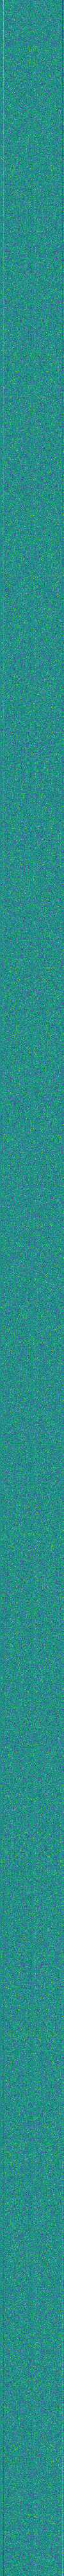
\includegraphics[interpolate=false,width=1.000000in,height=1.000000in]{antiderivative_ci_10-img0.png}}%
\end{pgfscope}%
\begin{pgfscope}%
\pgfsetbuttcap%
\pgfsetroundjoin%
\definecolor{currentfill}{rgb}{0.000000,0.000000,0.000000}%
\pgfsetfillcolor{currentfill}%
\pgfsetlinewidth{0.803000pt}%
\definecolor{currentstroke}{rgb}{0.000000,0.000000,0.000000}%
\pgfsetstrokecolor{currentstroke}%
\pgfsetdash{}{0pt}%
\pgfsys@defobject{currentmarker}{\pgfqpoint{0.000000in}{-0.048611in}}{\pgfqpoint{0.000000in}{0.000000in}}{%
\pgfpathmoveto{\pgfqpoint{0.000000in}{0.000000in}}%
\pgfpathlineto{\pgfqpoint{0.000000in}{-0.048611in}}%
\pgfusepath{stroke,fill}%
}%
\begin{pgfscope}%
\pgfsys@transformshift{0.800000in}{0.528000in}%
\pgfsys@useobject{currentmarker}{}%
\end{pgfscope}%
\end{pgfscope}%
\begin{pgfscope}%
\definecolor{textcolor}{rgb}{0.000000,0.000000,0.000000}%
\pgfsetstrokecolor{textcolor}%
\pgfsetfillcolor{textcolor}%
\pgftext[x=0.800000in,y=0.430778in,,top]{\color{textcolor}{\rmfamily\fontsize{12.000000}{14.400000}\selectfont\catcode`\^=\active\def^{\ifmmode\sp\else\^{}\fi}\catcode`\%=\active\def%{\%}0}}%
\end{pgfscope}%
\begin{pgfscope}%
\pgfsetbuttcap%
\pgfsetroundjoin%
\definecolor{currentfill}{rgb}{0.000000,0.000000,0.000000}%
\pgfsetfillcolor{currentfill}%
\pgfsetlinewidth{0.803000pt}%
\definecolor{currentstroke}{rgb}{0.000000,0.000000,0.000000}%
\pgfsetstrokecolor{currentstroke}%
\pgfsetdash{}{0pt}%
\pgfsys@defobject{currentmarker}{\pgfqpoint{0.000000in}{-0.048611in}}{\pgfqpoint{0.000000in}{0.000000in}}{%
\pgfpathmoveto{\pgfqpoint{0.000000in}{0.000000in}}%
\pgfpathlineto{\pgfqpoint{0.000000in}{-0.048611in}}%
\pgfusepath{stroke,fill}%
}%
\begin{pgfscope}%
\pgfsys@transformshift{1.593600in}{0.528000in}%
\pgfsys@useobject{currentmarker}{}%
\end{pgfscope}%
\end{pgfscope}%
\begin{pgfscope}%
\definecolor{textcolor}{rgb}{0.000000,0.000000,0.000000}%
\pgfsetstrokecolor{textcolor}%
\pgfsetfillcolor{textcolor}%
\pgftext[x=1.593600in,y=0.430778in,,top]{\color{textcolor}{\rmfamily\fontsize{12.000000}{14.400000}\selectfont\catcode`\^=\active\def^{\ifmmode\sp\else\^{}\fi}\catcode`\%=\active\def%{\%}10}}%
\end{pgfscope}%
\begin{pgfscope}%
\pgfsetbuttcap%
\pgfsetroundjoin%
\definecolor{currentfill}{rgb}{0.000000,0.000000,0.000000}%
\pgfsetfillcolor{currentfill}%
\pgfsetlinewidth{0.803000pt}%
\definecolor{currentstroke}{rgb}{0.000000,0.000000,0.000000}%
\pgfsetstrokecolor{currentstroke}%
\pgfsetdash{}{0pt}%
\pgfsys@defobject{currentmarker}{\pgfqpoint{0.000000in}{-0.048611in}}{\pgfqpoint{0.000000in}{0.000000in}}{%
\pgfpathmoveto{\pgfqpoint{0.000000in}{0.000000in}}%
\pgfpathlineto{\pgfqpoint{0.000000in}{-0.048611in}}%
\pgfusepath{stroke,fill}%
}%
\begin{pgfscope}%
\pgfsys@transformshift{2.387200in}{0.528000in}%
\pgfsys@useobject{currentmarker}{}%
\end{pgfscope}%
\end{pgfscope}%
\begin{pgfscope}%
\definecolor{textcolor}{rgb}{0.000000,0.000000,0.000000}%
\pgfsetstrokecolor{textcolor}%
\pgfsetfillcolor{textcolor}%
\pgftext[x=2.387200in,y=0.430778in,,top]{\color{textcolor}{\rmfamily\fontsize{12.000000}{14.400000}\selectfont\catcode`\^=\active\def^{\ifmmode\sp\else\^{}\fi}\catcode`\%=\active\def%{\%}20}}%
\end{pgfscope}%
\begin{pgfscope}%
\pgfsetbuttcap%
\pgfsetroundjoin%
\definecolor{currentfill}{rgb}{0.000000,0.000000,0.000000}%
\pgfsetfillcolor{currentfill}%
\pgfsetlinewidth{0.803000pt}%
\definecolor{currentstroke}{rgb}{0.000000,0.000000,0.000000}%
\pgfsetstrokecolor{currentstroke}%
\pgfsetdash{}{0pt}%
\pgfsys@defobject{currentmarker}{\pgfqpoint{0.000000in}{-0.048611in}}{\pgfqpoint{0.000000in}{0.000000in}}{%
\pgfpathmoveto{\pgfqpoint{0.000000in}{0.000000in}}%
\pgfpathlineto{\pgfqpoint{0.000000in}{-0.048611in}}%
\pgfusepath{stroke,fill}%
}%
\begin{pgfscope}%
\pgfsys@transformshift{3.180800in}{0.528000in}%
\pgfsys@useobject{currentmarker}{}%
\end{pgfscope}%
\end{pgfscope}%
\begin{pgfscope}%
\definecolor{textcolor}{rgb}{0.000000,0.000000,0.000000}%
\pgfsetstrokecolor{textcolor}%
\pgfsetfillcolor{textcolor}%
\pgftext[x=3.180800in,y=0.430778in,,top]{\color{textcolor}{\rmfamily\fontsize{12.000000}{14.400000}\selectfont\catcode`\^=\active\def^{\ifmmode\sp\else\^{}\fi}\catcode`\%=\active\def%{\%}30}}%
\end{pgfscope}%
\begin{pgfscope}%
\pgfsetbuttcap%
\pgfsetroundjoin%
\definecolor{currentfill}{rgb}{0.000000,0.000000,0.000000}%
\pgfsetfillcolor{currentfill}%
\pgfsetlinewidth{0.803000pt}%
\definecolor{currentstroke}{rgb}{0.000000,0.000000,0.000000}%
\pgfsetstrokecolor{currentstroke}%
\pgfsetdash{}{0pt}%
\pgfsys@defobject{currentmarker}{\pgfqpoint{0.000000in}{-0.048611in}}{\pgfqpoint{0.000000in}{0.000000in}}{%
\pgfpathmoveto{\pgfqpoint{0.000000in}{0.000000in}}%
\pgfpathlineto{\pgfqpoint{0.000000in}{-0.048611in}}%
\pgfusepath{stroke,fill}%
}%
\begin{pgfscope}%
\pgfsys@transformshift{3.974400in}{0.528000in}%
\pgfsys@useobject{currentmarker}{}%
\end{pgfscope}%
\end{pgfscope}%
\begin{pgfscope}%
\definecolor{textcolor}{rgb}{0.000000,0.000000,0.000000}%
\pgfsetstrokecolor{textcolor}%
\pgfsetfillcolor{textcolor}%
\pgftext[x=3.974400in,y=0.430778in,,top]{\color{textcolor}{\rmfamily\fontsize{12.000000}{14.400000}\selectfont\catcode`\^=\active\def^{\ifmmode\sp\else\^{}\fi}\catcode`\%=\active\def%{\%}40}}%
\end{pgfscope}%
\begin{pgfscope}%
\pgfsetbuttcap%
\pgfsetroundjoin%
\definecolor{currentfill}{rgb}{0.000000,0.000000,0.000000}%
\pgfsetfillcolor{currentfill}%
\pgfsetlinewidth{0.803000pt}%
\definecolor{currentstroke}{rgb}{0.000000,0.000000,0.000000}%
\pgfsetstrokecolor{currentstroke}%
\pgfsetdash{}{0pt}%
\pgfsys@defobject{currentmarker}{\pgfqpoint{0.000000in}{-0.048611in}}{\pgfqpoint{0.000000in}{0.000000in}}{%
\pgfpathmoveto{\pgfqpoint{0.000000in}{0.000000in}}%
\pgfpathlineto{\pgfqpoint{0.000000in}{-0.048611in}}%
\pgfusepath{stroke,fill}%
}%
\begin{pgfscope}%
\pgfsys@transformshift{4.768000in}{0.528000in}%
\pgfsys@useobject{currentmarker}{}%
\end{pgfscope}%
\end{pgfscope}%
\begin{pgfscope}%
\definecolor{textcolor}{rgb}{0.000000,0.000000,0.000000}%
\pgfsetstrokecolor{textcolor}%
\pgfsetfillcolor{textcolor}%
\pgftext[x=4.768000in,y=0.430778in,,top]{\color{textcolor}{\rmfamily\fontsize{12.000000}{14.400000}\selectfont\catcode`\^=\active\def^{\ifmmode\sp\else\^{}\fi}\catcode`\%=\active\def%{\%}50}}%
\end{pgfscope}%
\begin{pgfscope}%
\definecolor{textcolor}{rgb}{0.000000,0.000000,0.000000}%
\pgfsetstrokecolor{textcolor}%
\pgfsetfillcolor{textcolor}%
\pgftext[x=2.784000in,y=0.213927in,,top]{\color{textcolor}{\rmfamily\fontsize{12.000000}{14.400000}\selectfont\catcode`\^=\active\def^{\ifmmode\sp\else\^{}\fi}\catcode`\%=\active\def%{\%}input coefficients}}%
\end{pgfscope}%
\begin{pgfscope}%
\pgfsetbuttcap%
\pgfsetroundjoin%
\definecolor{currentfill}{rgb}{0.000000,0.000000,0.000000}%
\pgfsetfillcolor{currentfill}%
\pgfsetlinewidth{0.803000pt}%
\definecolor{currentstroke}{rgb}{0.000000,0.000000,0.000000}%
\pgfsetstrokecolor{currentstroke}%
\pgfsetdash{}{0pt}%
\pgfsys@defobject{currentmarker}{\pgfqpoint{-0.048611in}{0.000000in}}{\pgfqpoint{-0.000000in}{0.000000in}}{%
\pgfpathmoveto{\pgfqpoint{-0.000000in}{0.000000in}}%
\pgfpathlineto{\pgfqpoint{-0.048611in}{0.000000in}}%
\pgfusepath{stroke,fill}%
}%
\begin{pgfscope}%
\pgfsys@transformshift{0.800000in}{4.224000in}%
\pgfsys@useobject{currentmarker}{}%
\end{pgfscope}%
\end{pgfscope}%
\begin{pgfscope}%
\definecolor{textcolor}{rgb}{0.000000,0.000000,0.000000}%
\pgfsetstrokecolor{textcolor}%
\pgfsetfillcolor{textcolor}%
\pgftext[x=0.596739in, y=4.160686in, left, base]{\color{textcolor}{\rmfamily\fontsize{12.000000}{14.400000}\selectfont\catcode`\^=\active\def^{\ifmmode\sp\else\^{}\fi}\catcode`\%=\active\def%{\%}0}}%
\end{pgfscope}%
\begin{pgfscope}%
\pgfsetbuttcap%
\pgfsetroundjoin%
\definecolor{currentfill}{rgb}{0.000000,0.000000,0.000000}%
\pgfsetfillcolor{currentfill}%
\pgfsetlinewidth{0.803000pt}%
\definecolor{currentstroke}{rgb}{0.000000,0.000000,0.000000}%
\pgfsetstrokecolor{currentstroke}%
\pgfsetdash{}{0pt}%
\pgfsys@defobject{currentmarker}{\pgfqpoint{-0.048611in}{0.000000in}}{\pgfqpoint{-0.000000in}{0.000000in}}{%
\pgfpathmoveto{\pgfqpoint{-0.000000in}{0.000000in}}%
\pgfpathlineto{\pgfqpoint{-0.048611in}{0.000000in}}%
\pgfusepath{stroke,fill}%
}%
\begin{pgfscope}%
\pgfsys@transformshift{0.800000in}{3.762000in}%
\pgfsys@useobject{currentmarker}{}%
\end{pgfscope}%
\end{pgfscope}%
\begin{pgfscope}%
\definecolor{textcolor}{rgb}{0.000000,0.000000,0.000000}%
\pgfsetstrokecolor{textcolor}%
\pgfsetfillcolor{textcolor}%
\pgftext[x=0.384662in, y=3.698686in, left, base]{\color{textcolor}{\rmfamily\fontsize{12.000000}{14.400000}\selectfont\catcode`\^=\active\def^{\ifmmode\sp\else\^{}\fi}\catcode`\%=\active\def%{\%}500}}%
\end{pgfscope}%
\begin{pgfscope}%
\pgfsetbuttcap%
\pgfsetroundjoin%
\definecolor{currentfill}{rgb}{0.000000,0.000000,0.000000}%
\pgfsetfillcolor{currentfill}%
\pgfsetlinewidth{0.803000pt}%
\definecolor{currentstroke}{rgb}{0.000000,0.000000,0.000000}%
\pgfsetstrokecolor{currentstroke}%
\pgfsetdash{}{0pt}%
\pgfsys@defobject{currentmarker}{\pgfqpoint{-0.048611in}{0.000000in}}{\pgfqpoint{-0.000000in}{0.000000in}}{%
\pgfpathmoveto{\pgfqpoint{-0.000000in}{0.000000in}}%
\pgfpathlineto{\pgfqpoint{-0.048611in}{0.000000in}}%
\pgfusepath{stroke,fill}%
}%
\begin{pgfscope}%
\pgfsys@transformshift{0.800000in}{3.300000in}%
\pgfsys@useobject{currentmarker}{}%
\end{pgfscope}%
\end{pgfscope}%
\begin{pgfscope}%
\definecolor{textcolor}{rgb}{0.000000,0.000000,0.000000}%
\pgfsetstrokecolor{textcolor}%
\pgfsetfillcolor{textcolor}%
\pgftext[x=0.278624in, y=3.236686in, left, base]{\color{textcolor}{\rmfamily\fontsize{12.000000}{14.400000}\selectfont\catcode`\^=\active\def^{\ifmmode\sp\else\^{}\fi}\catcode`\%=\active\def%{\%}1000}}%
\end{pgfscope}%
\begin{pgfscope}%
\pgfsetbuttcap%
\pgfsetroundjoin%
\definecolor{currentfill}{rgb}{0.000000,0.000000,0.000000}%
\pgfsetfillcolor{currentfill}%
\pgfsetlinewidth{0.803000pt}%
\definecolor{currentstroke}{rgb}{0.000000,0.000000,0.000000}%
\pgfsetstrokecolor{currentstroke}%
\pgfsetdash{}{0pt}%
\pgfsys@defobject{currentmarker}{\pgfqpoint{-0.048611in}{0.000000in}}{\pgfqpoint{-0.000000in}{0.000000in}}{%
\pgfpathmoveto{\pgfqpoint{-0.000000in}{0.000000in}}%
\pgfpathlineto{\pgfqpoint{-0.048611in}{0.000000in}}%
\pgfusepath{stroke,fill}%
}%
\begin{pgfscope}%
\pgfsys@transformshift{0.800000in}{2.838000in}%
\pgfsys@useobject{currentmarker}{}%
\end{pgfscope}%
\end{pgfscope}%
\begin{pgfscope}%
\definecolor{textcolor}{rgb}{0.000000,0.000000,0.000000}%
\pgfsetstrokecolor{textcolor}%
\pgfsetfillcolor{textcolor}%
\pgftext[x=0.278624in, y=2.774686in, left, base]{\color{textcolor}{\rmfamily\fontsize{12.000000}{14.400000}\selectfont\catcode`\^=\active\def^{\ifmmode\sp\else\^{}\fi}\catcode`\%=\active\def%{\%}1500}}%
\end{pgfscope}%
\begin{pgfscope}%
\pgfsetbuttcap%
\pgfsetroundjoin%
\definecolor{currentfill}{rgb}{0.000000,0.000000,0.000000}%
\pgfsetfillcolor{currentfill}%
\pgfsetlinewidth{0.803000pt}%
\definecolor{currentstroke}{rgb}{0.000000,0.000000,0.000000}%
\pgfsetstrokecolor{currentstroke}%
\pgfsetdash{}{0pt}%
\pgfsys@defobject{currentmarker}{\pgfqpoint{-0.048611in}{0.000000in}}{\pgfqpoint{-0.000000in}{0.000000in}}{%
\pgfpathmoveto{\pgfqpoint{-0.000000in}{0.000000in}}%
\pgfpathlineto{\pgfqpoint{-0.048611in}{0.000000in}}%
\pgfusepath{stroke,fill}%
}%
\begin{pgfscope}%
\pgfsys@transformshift{0.800000in}{2.376000in}%
\pgfsys@useobject{currentmarker}{}%
\end{pgfscope}%
\end{pgfscope}%
\begin{pgfscope}%
\definecolor{textcolor}{rgb}{0.000000,0.000000,0.000000}%
\pgfsetstrokecolor{textcolor}%
\pgfsetfillcolor{textcolor}%
\pgftext[x=0.278624in, y=2.312686in, left, base]{\color{textcolor}{\rmfamily\fontsize{12.000000}{14.400000}\selectfont\catcode`\^=\active\def^{\ifmmode\sp\else\^{}\fi}\catcode`\%=\active\def%{\%}2000}}%
\end{pgfscope}%
\begin{pgfscope}%
\pgfsetbuttcap%
\pgfsetroundjoin%
\definecolor{currentfill}{rgb}{0.000000,0.000000,0.000000}%
\pgfsetfillcolor{currentfill}%
\pgfsetlinewidth{0.803000pt}%
\definecolor{currentstroke}{rgb}{0.000000,0.000000,0.000000}%
\pgfsetstrokecolor{currentstroke}%
\pgfsetdash{}{0pt}%
\pgfsys@defobject{currentmarker}{\pgfqpoint{-0.048611in}{0.000000in}}{\pgfqpoint{-0.000000in}{0.000000in}}{%
\pgfpathmoveto{\pgfqpoint{-0.000000in}{0.000000in}}%
\pgfpathlineto{\pgfqpoint{-0.048611in}{0.000000in}}%
\pgfusepath{stroke,fill}%
}%
\begin{pgfscope}%
\pgfsys@transformshift{0.800000in}{1.914000in}%
\pgfsys@useobject{currentmarker}{}%
\end{pgfscope}%
\end{pgfscope}%
\begin{pgfscope}%
\definecolor{textcolor}{rgb}{0.000000,0.000000,0.000000}%
\pgfsetstrokecolor{textcolor}%
\pgfsetfillcolor{textcolor}%
\pgftext[x=0.278624in, y=1.850686in, left, base]{\color{textcolor}{\rmfamily\fontsize{12.000000}{14.400000}\selectfont\catcode`\^=\active\def^{\ifmmode\sp\else\^{}\fi}\catcode`\%=\active\def%{\%}2500}}%
\end{pgfscope}%
\begin{pgfscope}%
\pgfsetbuttcap%
\pgfsetroundjoin%
\definecolor{currentfill}{rgb}{0.000000,0.000000,0.000000}%
\pgfsetfillcolor{currentfill}%
\pgfsetlinewidth{0.803000pt}%
\definecolor{currentstroke}{rgb}{0.000000,0.000000,0.000000}%
\pgfsetstrokecolor{currentstroke}%
\pgfsetdash{}{0pt}%
\pgfsys@defobject{currentmarker}{\pgfqpoint{-0.048611in}{0.000000in}}{\pgfqpoint{-0.000000in}{0.000000in}}{%
\pgfpathmoveto{\pgfqpoint{-0.000000in}{0.000000in}}%
\pgfpathlineto{\pgfqpoint{-0.048611in}{0.000000in}}%
\pgfusepath{stroke,fill}%
}%
\begin{pgfscope}%
\pgfsys@transformshift{0.800000in}{1.452000in}%
\pgfsys@useobject{currentmarker}{}%
\end{pgfscope}%
\end{pgfscope}%
\begin{pgfscope}%
\definecolor{textcolor}{rgb}{0.000000,0.000000,0.000000}%
\pgfsetstrokecolor{textcolor}%
\pgfsetfillcolor{textcolor}%
\pgftext[x=0.278624in, y=1.388686in, left, base]{\color{textcolor}{\rmfamily\fontsize{12.000000}{14.400000}\selectfont\catcode`\^=\active\def^{\ifmmode\sp\else\^{}\fi}\catcode`\%=\active\def%{\%}3000}}%
\end{pgfscope}%
\begin{pgfscope}%
\pgfsetbuttcap%
\pgfsetroundjoin%
\definecolor{currentfill}{rgb}{0.000000,0.000000,0.000000}%
\pgfsetfillcolor{currentfill}%
\pgfsetlinewidth{0.803000pt}%
\definecolor{currentstroke}{rgb}{0.000000,0.000000,0.000000}%
\pgfsetstrokecolor{currentstroke}%
\pgfsetdash{}{0pt}%
\pgfsys@defobject{currentmarker}{\pgfqpoint{-0.048611in}{0.000000in}}{\pgfqpoint{-0.000000in}{0.000000in}}{%
\pgfpathmoveto{\pgfqpoint{-0.000000in}{0.000000in}}%
\pgfpathlineto{\pgfqpoint{-0.048611in}{0.000000in}}%
\pgfusepath{stroke,fill}%
}%
\begin{pgfscope}%
\pgfsys@transformshift{0.800000in}{0.990000in}%
\pgfsys@useobject{currentmarker}{}%
\end{pgfscope}%
\end{pgfscope}%
\begin{pgfscope}%
\definecolor{textcolor}{rgb}{0.000000,0.000000,0.000000}%
\pgfsetstrokecolor{textcolor}%
\pgfsetfillcolor{textcolor}%
\pgftext[x=0.278624in, y=0.926686in, left, base]{\color{textcolor}{\rmfamily\fontsize{12.000000}{14.400000}\selectfont\catcode`\^=\active\def^{\ifmmode\sp\else\^{}\fi}\catcode`\%=\active\def%{\%}3500}}%
\end{pgfscope}%
\begin{pgfscope}%
\pgfsetbuttcap%
\pgfsetroundjoin%
\definecolor{currentfill}{rgb}{0.000000,0.000000,0.000000}%
\pgfsetfillcolor{currentfill}%
\pgfsetlinewidth{0.803000pt}%
\definecolor{currentstroke}{rgb}{0.000000,0.000000,0.000000}%
\pgfsetstrokecolor{currentstroke}%
\pgfsetdash{}{0pt}%
\pgfsys@defobject{currentmarker}{\pgfqpoint{-0.048611in}{0.000000in}}{\pgfqpoint{-0.000000in}{0.000000in}}{%
\pgfpathmoveto{\pgfqpoint{-0.000000in}{0.000000in}}%
\pgfpathlineto{\pgfqpoint{-0.048611in}{0.000000in}}%
\pgfusepath{stroke,fill}%
}%
\begin{pgfscope}%
\pgfsys@transformshift{0.800000in}{0.528000in}%
\pgfsys@useobject{currentmarker}{}%
\end{pgfscope}%
\end{pgfscope}%
\begin{pgfscope}%
\definecolor{textcolor}{rgb}{0.000000,0.000000,0.000000}%
\pgfsetstrokecolor{textcolor}%
\pgfsetfillcolor{textcolor}%
\pgftext[x=0.278624in, y=0.464686in, left, base]{\color{textcolor}{\rmfamily\fontsize{12.000000}{14.400000}\selectfont\catcode`\^=\active\def^{\ifmmode\sp\else\^{}\fi}\catcode`\%=\active\def%{\%}4000}}%
\end{pgfscope}%
\begin{pgfscope}%
\definecolor{textcolor}{rgb}{0.000000,0.000000,0.000000}%
\pgfsetstrokecolor{textcolor}%
\pgfsetfillcolor{textcolor}%
\pgftext[x=0.223069in,y=2.376000in,,bottom,rotate=90.000000]{\color{textcolor}{\rmfamily\fontsize{12.000000}{14.400000}\selectfont\catcode`\^=\active\def^{\ifmmode\sp\else\^{}\fi}\catcode`\%=\active\def%{\%}samples}}%
\end{pgfscope}%
\begin{pgfscope}%
\pgfsetrectcap%
\pgfsetmiterjoin%
\pgfsetlinewidth{0.803000pt}%
\definecolor{currentstroke}{rgb}{0.000000,0.000000,0.000000}%
\pgfsetstrokecolor{currentstroke}%
\pgfsetdash{}{0pt}%
\pgfpathmoveto{\pgfqpoint{0.800000in}{0.528000in}}%
\pgfpathlineto{\pgfqpoint{0.800000in}{4.224000in}}%
\pgfusepath{stroke}%
\end{pgfscope}%
\begin{pgfscope}%
\pgfsetrectcap%
\pgfsetmiterjoin%
\pgfsetlinewidth{0.803000pt}%
\definecolor{currentstroke}{rgb}{0.000000,0.000000,0.000000}%
\pgfsetstrokecolor{currentstroke}%
\pgfsetdash{}{0pt}%
\pgfpathmoveto{\pgfqpoint{4.768000in}{0.528000in}}%
\pgfpathlineto{\pgfqpoint{4.768000in}{4.224000in}}%
\pgfusepath{stroke}%
\end{pgfscope}%
\begin{pgfscope}%
\pgfsetrectcap%
\pgfsetmiterjoin%
\pgfsetlinewidth{0.803000pt}%
\definecolor{currentstroke}{rgb}{0.000000,0.000000,0.000000}%
\pgfsetstrokecolor{currentstroke}%
\pgfsetdash{}{0pt}%
\pgfpathmoveto{\pgfqpoint{0.800000in}{0.528000in}}%
\pgfpathlineto{\pgfqpoint{4.768000in}{0.528000in}}%
\pgfusepath{stroke}%
\end{pgfscope}%
\begin{pgfscope}%
\pgfsetrectcap%
\pgfsetmiterjoin%
\pgfsetlinewidth{0.803000pt}%
\definecolor{currentstroke}{rgb}{0.000000,0.000000,0.000000}%
\pgfsetstrokecolor{currentstroke}%
\pgfsetdash{}{0pt}%
\pgfpathmoveto{\pgfqpoint{0.800000in}{4.224000in}}%
\pgfpathlineto{\pgfqpoint{4.768000in}{4.224000in}}%
\pgfusepath{stroke}%
\end{pgfscope}%
\begin{pgfscope}%
\pgfsetbuttcap%
\pgfsetmiterjoin%
\pgfsetlinewidth{0.000000pt}%
\definecolor{currentstroke}{rgb}{0.000000,0.000000,0.000000}%
\pgfsetstrokecolor{currentstroke}%
\pgfsetstrokeopacity{0.000000}%
\pgfsetdash{}{0pt}%
\pgfpathmoveto{\pgfqpoint{5.016000in}{0.528000in}}%
\pgfpathlineto{\pgfqpoint{5.200800in}{0.528000in}}%
\pgfpathlineto{\pgfqpoint{5.200800in}{4.224000in}}%
\pgfpathlineto{\pgfqpoint{5.016000in}{4.224000in}}%
\pgfpathlineto{\pgfqpoint{5.016000in}{0.528000in}}%
\pgfpathclose%
\pgfusepath{}%
\end{pgfscope}%
\begin{pgfscope}%
\pgfsys@transformshift{5.020000in}{0.530000in}%
\pgftext[left,bottom]{
\includegraphics[interpolate=true,width=0.180000in,height=3.690000in]{antiderivative_ci_10-img1.png}}%
\end{pgfscope}%
\begin{pgfscope}%
\pgfsetbuttcap%
\pgfsetroundjoin%
\definecolor{currentfill}{rgb}{0.000000,0.000000,0.000000}%
\pgfsetfillcolor{currentfill}%
\pgfsetlinewidth{0.803000pt}%
\definecolor{currentstroke}{rgb}{0.000000,0.000000,0.000000}%
\pgfsetstrokecolor{currentstroke}%
\pgfsetdash{}{0pt}%
\pgfsys@defobject{currentmarker}{\pgfqpoint{0.000000in}{0.000000in}}{\pgfqpoint{0.048611in}{0.000000in}}{%
\pgfpathmoveto{\pgfqpoint{0.000000in}{0.000000in}}%
\pgfpathlineto{\pgfqpoint{0.048611in}{0.000000in}}%
\pgfusepath{stroke,fill}%
}%
\begin{pgfscope}%
\pgfsys@transformshift{5.200800in}{0.547966in}%
\pgfsys@useobject{currentmarker}{}%
\end{pgfscope}%
\end{pgfscope}%
\begin{pgfscope}%
\definecolor{textcolor}{rgb}{0.000000,0.000000,0.000000}%
\pgfsetstrokecolor{textcolor}%
\pgfsetfillcolor{textcolor}%
\pgftext[x=5.298022in, y=0.484652in, left, base]{\color{textcolor}{\rmfamily\fontsize{12.000000}{14.400000}\selectfont\catcode`\^=\active\def^{\ifmmode\sp\else\^{}\fi}\catcode`\%=\active\def%{\%}\ensuremath{-}100}}%
\end{pgfscope}%
\begin{pgfscope}%
\pgfsetbuttcap%
\pgfsetroundjoin%
\definecolor{currentfill}{rgb}{0.000000,0.000000,0.000000}%
\pgfsetfillcolor{currentfill}%
\pgfsetlinewidth{0.803000pt}%
\definecolor{currentstroke}{rgb}{0.000000,0.000000,0.000000}%
\pgfsetstrokecolor{currentstroke}%
\pgfsetdash{}{0pt}%
\pgfsys@defobject{currentmarker}{\pgfqpoint{0.000000in}{0.000000in}}{\pgfqpoint{0.048611in}{0.000000in}}{%
\pgfpathmoveto{\pgfqpoint{0.000000in}{0.000000in}}%
\pgfpathlineto{\pgfqpoint{0.048611in}{0.000000in}}%
\pgfusepath{stroke,fill}%
}%
\begin{pgfscope}%
\pgfsys@transformshift{5.200800in}{0.998231in}%
\pgfsys@useobject{currentmarker}{}%
\end{pgfscope}%
\end{pgfscope}%
\begin{pgfscope}%
\definecolor{textcolor}{rgb}{0.000000,0.000000,0.000000}%
\pgfsetstrokecolor{textcolor}%
\pgfsetfillcolor{textcolor}%
\pgftext[x=5.298022in, y=0.934917in, left, base]{\color{textcolor}{\rmfamily\fontsize{12.000000}{14.400000}\selectfont\catcode`\^=\active\def^{\ifmmode\sp\else\^{}\fi}\catcode`\%=\active\def%{\%}\ensuremath{-}75}}%
\end{pgfscope}%
\begin{pgfscope}%
\pgfsetbuttcap%
\pgfsetroundjoin%
\definecolor{currentfill}{rgb}{0.000000,0.000000,0.000000}%
\pgfsetfillcolor{currentfill}%
\pgfsetlinewidth{0.803000pt}%
\definecolor{currentstroke}{rgb}{0.000000,0.000000,0.000000}%
\pgfsetstrokecolor{currentstroke}%
\pgfsetdash{}{0pt}%
\pgfsys@defobject{currentmarker}{\pgfqpoint{0.000000in}{0.000000in}}{\pgfqpoint{0.048611in}{0.000000in}}{%
\pgfpathmoveto{\pgfqpoint{0.000000in}{0.000000in}}%
\pgfpathlineto{\pgfqpoint{0.048611in}{0.000000in}}%
\pgfusepath{stroke,fill}%
}%
\begin{pgfscope}%
\pgfsys@transformshift{5.200800in}{1.448497in}%
\pgfsys@useobject{currentmarker}{}%
\end{pgfscope}%
\end{pgfscope}%
\begin{pgfscope}%
\definecolor{textcolor}{rgb}{0.000000,0.000000,0.000000}%
\pgfsetstrokecolor{textcolor}%
\pgfsetfillcolor{textcolor}%
\pgftext[x=5.298022in, y=1.385183in, left, base]{\color{textcolor}{\rmfamily\fontsize{12.000000}{14.400000}\selectfont\catcode`\^=\active\def^{\ifmmode\sp\else\^{}\fi}\catcode`\%=\active\def%{\%}\ensuremath{-}50}}%
\end{pgfscope}%
\begin{pgfscope}%
\pgfsetbuttcap%
\pgfsetroundjoin%
\definecolor{currentfill}{rgb}{0.000000,0.000000,0.000000}%
\pgfsetfillcolor{currentfill}%
\pgfsetlinewidth{0.803000pt}%
\definecolor{currentstroke}{rgb}{0.000000,0.000000,0.000000}%
\pgfsetstrokecolor{currentstroke}%
\pgfsetdash{}{0pt}%
\pgfsys@defobject{currentmarker}{\pgfqpoint{0.000000in}{0.000000in}}{\pgfqpoint{0.048611in}{0.000000in}}{%
\pgfpathmoveto{\pgfqpoint{0.000000in}{0.000000in}}%
\pgfpathlineto{\pgfqpoint{0.048611in}{0.000000in}}%
\pgfusepath{stroke,fill}%
}%
\begin{pgfscope}%
\pgfsys@transformshift{5.200800in}{1.898762in}%
\pgfsys@useobject{currentmarker}{}%
\end{pgfscope}%
\end{pgfscope}%
\begin{pgfscope}%
\definecolor{textcolor}{rgb}{0.000000,0.000000,0.000000}%
\pgfsetstrokecolor{textcolor}%
\pgfsetfillcolor{textcolor}%
\pgftext[x=5.298022in, y=1.835448in, left, base]{\color{textcolor}{\rmfamily\fontsize{12.000000}{14.400000}\selectfont\catcode`\^=\active\def^{\ifmmode\sp\else\^{}\fi}\catcode`\%=\active\def%{\%}\ensuremath{-}25}}%
\end{pgfscope}%
\begin{pgfscope}%
\pgfsetbuttcap%
\pgfsetroundjoin%
\definecolor{currentfill}{rgb}{0.000000,0.000000,0.000000}%
\pgfsetfillcolor{currentfill}%
\pgfsetlinewidth{0.803000pt}%
\definecolor{currentstroke}{rgb}{0.000000,0.000000,0.000000}%
\pgfsetstrokecolor{currentstroke}%
\pgfsetdash{}{0pt}%
\pgfsys@defobject{currentmarker}{\pgfqpoint{0.000000in}{0.000000in}}{\pgfqpoint{0.048611in}{0.000000in}}{%
\pgfpathmoveto{\pgfqpoint{0.000000in}{0.000000in}}%
\pgfpathlineto{\pgfqpoint{0.048611in}{0.000000in}}%
\pgfusepath{stroke,fill}%
}%
\begin{pgfscope}%
\pgfsys@transformshift{5.200800in}{2.349028in}%
\pgfsys@useobject{currentmarker}{}%
\end{pgfscope}%
\end{pgfscope}%
\begin{pgfscope}%
\definecolor{textcolor}{rgb}{0.000000,0.000000,0.000000}%
\pgfsetstrokecolor{textcolor}%
\pgfsetfillcolor{textcolor}%
\pgftext[x=5.298022in, y=2.285714in, left, base]{\color{textcolor}{\rmfamily\fontsize{12.000000}{14.400000}\selectfont\catcode`\^=\active\def^{\ifmmode\sp\else\^{}\fi}\catcode`\%=\active\def%{\%}0}}%
\end{pgfscope}%
\begin{pgfscope}%
\pgfsetbuttcap%
\pgfsetroundjoin%
\definecolor{currentfill}{rgb}{0.000000,0.000000,0.000000}%
\pgfsetfillcolor{currentfill}%
\pgfsetlinewidth{0.803000pt}%
\definecolor{currentstroke}{rgb}{0.000000,0.000000,0.000000}%
\pgfsetstrokecolor{currentstroke}%
\pgfsetdash{}{0pt}%
\pgfsys@defobject{currentmarker}{\pgfqpoint{0.000000in}{0.000000in}}{\pgfqpoint{0.048611in}{0.000000in}}{%
\pgfpathmoveto{\pgfqpoint{0.000000in}{0.000000in}}%
\pgfpathlineto{\pgfqpoint{0.048611in}{0.000000in}}%
\pgfusepath{stroke,fill}%
}%
\begin{pgfscope}%
\pgfsys@transformshift{5.200800in}{2.799293in}%
\pgfsys@useobject{currentmarker}{}%
\end{pgfscope}%
\end{pgfscope}%
\begin{pgfscope}%
\definecolor{textcolor}{rgb}{0.000000,0.000000,0.000000}%
\pgfsetstrokecolor{textcolor}%
\pgfsetfillcolor{textcolor}%
\pgftext[x=5.298022in, y=2.735979in, left, base]{\color{textcolor}{\rmfamily\fontsize{12.000000}{14.400000}\selectfont\catcode`\^=\active\def^{\ifmmode\sp\else\^{}\fi}\catcode`\%=\active\def%{\%}25}}%
\end{pgfscope}%
\begin{pgfscope}%
\pgfsetbuttcap%
\pgfsetroundjoin%
\definecolor{currentfill}{rgb}{0.000000,0.000000,0.000000}%
\pgfsetfillcolor{currentfill}%
\pgfsetlinewidth{0.803000pt}%
\definecolor{currentstroke}{rgb}{0.000000,0.000000,0.000000}%
\pgfsetstrokecolor{currentstroke}%
\pgfsetdash{}{0pt}%
\pgfsys@defobject{currentmarker}{\pgfqpoint{0.000000in}{0.000000in}}{\pgfqpoint{0.048611in}{0.000000in}}{%
\pgfpathmoveto{\pgfqpoint{0.000000in}{0.000000in}}%
\pgfpathlineto{\pgfqpoint{0.048611in}{0.000000in}}%
\pgfusepath{stroke,fill}%
}%
\begin{pgfscope}%
\pgfsys@transformshift{5.200800in}{3.249559in}%
\pgfsys@useobject{currentmarker}{}%
\end{pgfscope}%
\end{pgfscope}%
\begin{pgfscope}%
\definecolor{textcolor}{rgb}{0.000000,0.000000,0.000000}%
\pgfsetstrokecolor{textcolor}%
\pgfsetfillcolor{textcolor}%
\pgftext[x=5.298022in, y=3.186245in, left, base]{\color{textcolor}{\rmfamily\fontsize{12.000000}{14.400000}\selectfont\catcode`\^=\active\def^{\ifmmode\sp\else\^{}\fi}\catcode`\%=\active\def%{\%}50}}%
\end{pgfscope}%
\begin{pgfscope}%
\pgfsetbuttcap%
\pgfsetroundjoin%
\definecolor{currentfill}{rgb}{0.000000,0.000000,0.000000}%
\pgfsetfillcolor{currentfill}%
\pgfsetlinewidth{0.803000pt}%
\definecolor{currentstroke}{rgb}{0.000000,0.000000,0.000000}%
\pgfsetstrokecolor{currentstroke}%
\pgfsetdash{}{0pt}%
\pgfsys@defobject{currentmarker}{\pgfqpoint{0.000000in}{0.000000in}}{\pgfqpoint{0.048611in}{0.000000in}}{%
\pgfpathmoveto{\pgfqpoint{0.000000in}{0.000000in}}%
\pgfpathlineto{\pgfqpoint{0.048611in}{0.000000in}}%
\pgfusepath{stroke,fill}%
}%
\begin{pgfscope}%
\pgfsys@transformshift{5.200800in}{3.699824in}%
\pgfsys@useobject{currentmarker}{}%
\end{pgfscope}%
\end{pgfscope}%
\begin{pgfscope}%
\definecolor{textcolor}{rgb}{0.000000,0.000000,0.000000}%
\pgfsetstrokecolor{textcolor}%
\pgfsetfillcolor{textcolor}%
\pgftext[x=5.298022in, y=3.636510in, left, base]{\color{textcolor}{\rmfamily\fontsize{12.000000}{14.400000}\selectfont\catcode`\^=\active\def^{\ifmmode\sp\else\^{}\fi}\catcode`\%=\active\def%{\%}75}}%
\end{pgfscope}%
\begin{pgfscope}%
\pgfsetbuttcap%
\pgfsetroundjoin%
\definecolor{currentfill}{rgb}{0.000000,0.000000,0.000000}%
\pgfsetfillcolor{currentfill}%
\pgfsetlinewidth{0.803000pt}%
\definecolor{currentstroke}{rgb}{0.000000,0.000000,0.000000}%
\pgfsetstrokecolor{currentstroke}%
\pgfsetdash{}{0pt}%
\pgfsys@defobject{currentmarker}{\pgfqpoint{0.000000in}{0.000000in}}{\pgfqpoint{0.048611in}{0.000000in}}{%
\pgfpathmoveto{\pgfqpoint{0.000000in}{0.000000in}}%
\pgfpathlineto{\pgfqpoint{0.048611in}{0.000000in}}%
\pgfusepath{stroke,fill}%
}%
\begin{pgfscope}%
\pgfsys@transformshift{5.200800in}{4.150090in}%
\pgfsys@useobject{currentmarker}{}%
\end{pgfscope}%
\end{pgfscope}%
\begin{pgfscope}%
\definecolor{textcolor}{rgb}{0.000000,0.000000,0.000000}%
\pgfsetstrokecolor{textcolor}%
\pgfsetfillcolor{textcolor}%
\pgftext[x=5.298022in, y=4.086776in, left, base]{\color{textcolor}{\rmfamily\fontsize{12.000000}{14.400000}\selectfont\catcode`\^=\active\def^{\ifmmode\sp\else\^{}\fi}\catcode`\%=\active\def%{\%}100}}%
\end{pgfscope}%
\begin{pgfscope}%
\pgfsetrectcap%
\pgfsetmiterjoin%
\pgfsetlinewidth{0.803000pt}%
\definecolor{currentstroke}{rgb}{0.000000,0.000000,0.000000}%
\pgfsetstrokecolor{currentstroke}%
\pgfsetdash{}{0pt}%
\pgfpathmoveto{\pgfqpoint{5.016000in}{0.528000in}}%
\pgfpathlineto{\pgfqpoint{5.108400in}{0.528000in}}%
\pgfpathlineto{\pgfqpoint{5.200800in}{0.528000in}}%
\pgfpathlineto{\pgfqpoint{5.200800in}{4.224000in}}%
\pgfpathlineto{\pgfqpoint{5.108400in}{4.224000in}}%
\pgfpathlineto{\pgfqpoint{5.016000in}{4.224000in}}%
\pgfpathlineto{\pgfqpoint{5.016000in}{0.528000in}}%
\pgfpathclose%
\pgfusepath{stroke}%
\end{pgfscope}%
\end{pgfpicture}%
\makeatother%
\endgroup%

    \end{adjustbox}
    \caption{Correlation image 10\% noise.}\label{fig:sc1_ci_10}
  \end{subfigure}
  \begin{subfigure}{0.49\linewidth}
    \begin{adjustbox}{width=1.2\linewidth}
      \begingroup%
\makeatletter%
\begin{pgfpicture}%
\pgfpathrectangle{\pgfpointorigin}{\pgfqpoint{4.000000in}{3.000000in}}%
\pgfusepath{use as bounding box, clip}%
\begin{pgfscope}%
\pgfsetbuttcap%
\pgfsetmiterjoin%
\pgfsetlinewidth{0.000000pt}%
\definecolor{currentstroke}{rgb}{0.000000,0.000000,0.000000}%
\pgfsetstrokecolor{currentstroke}%
\pgfsetstrokeopacity{0.000000}%
\pgfsetdash{}{0pt}%
\pgfpathmoveto{\pgfqpoint{0.000000in}{0.000000in}}%
\pgfpathlineto{\pgfqpoint{4.000000in}{0.000000in}}%
\pgfpathlineto{\pgfqpoint{4.000000in}{3.000000in}}%
\pgfpathlineto{\pgfqpoint{0.000000in}{3.000000in}}%
\pgfpathlineto{\pgfqpoint{0.000000in}{0.000000in}}%
\pgfpathclose%
\pgfusepath{}%
\end{pgfscope}%
\begin{pgfscope}%
\pgfsetbuttcap%
\pgfsetmiterjoin%
\pgfsetlinewidth{0.000000pt}%
\definecolor{currentstroke}{rgb}{0.000000,0.000000,0.000000}%
\pgfsetstrokecolor{currentstroke}%
\pgfsetstrokeopacity{0.000000}%
\pgfsetdash{}{0pt}%
\pgfpathmoveto{\pgfqpoint{0.642156in}{0.517039in}}%
\pgfpathlineto{\pgfqpoint{3.032083in}{0.517039in}}%
\pgfpathlineto{\pgfqpoint{3.032083in}{2.906966in}}%
\pgfpathlineto{\pgfqpoint{0.642156in}{2.906966in}}%
\pgfpathlineto{\pgfqpoint{0.642156in}{0.517039in}}%
\pgfpathclose%
\pgfusepath{}%
\end{pgfscope}%
\begin{pgfscope}%
\pgfpathrectangle{\pgfqpoint{0.642156in}{0.517039in}}{\pgfqpoint{2.389927in}{2.389927in}}%
\pgfusepath{clip}%
\pgfsys@transformcm{2.389927}{0.000000}{0.000000}{-2.389927}{0.642156in}{2.906966in}%
\pgftext[left,bottom]{
\includegraphics[interpolate=false,width=1.000000in,height=1.000000in]{antiderivative_pm_10-img0.png}}%
\end{pgfscope}%
\begin{pgfscope}%
\pgfsetbuttcap%
\pgfsetroundjoin%
\definecolor{currentfill}{rgb}{0.000000,0.000000,0.000000}%
\pgfsetfillcolor{currentfill}%
\pgfsetlinewidth{0.803000pt}%
\definecolor{currentstroke}{rgb}{0.000000,0.000000,0.000000}%
\pgfsetstrokecolor{currentstroke}%
\pgfsetdash{}{0pt}%
\pgfsys@defobject{currentmarker}{\pgfqpoint{0.000000in}{-0.048611in}}{\pgfqpoint{0.000000in}{0.000000in}}{%
\pgfpathmoveto{\pgfqpoint{0.000000in}{0.000000in}}%
\pgfpathlineto{\pgfqpoint{0.000000in}{-0.048611in}}%
\pgfusepath{stroke,fill}%
}%
\begin{pgfscope}%
\pgfsys@transformshift{0.654106in}{0.517039in}%
\pgfsys@useobject{currentmarker}{}%
\end{pgfscope}%
\end{pgfscope}%
\begin{pgfscope}%
\definecolor{textcolor}{rgb}{0.000000,0.000000,0.000000}%
\pgfsetstrokecolor{textcolor}%
\pgfsetfillcolor{textcolor}%
\pgftext[x=0.654106in,y=0.419816in,,top]{\color{textcolor}{\rmfamily\fontsize{12.000000}{14.400000}\selectfont\catcode`\^=\active\def^{\ifmmode\sp\else\^{}\fi}\catcode`\%=\active\def%{\%}0}}%
\end{pgfscope}%
\begin{pgfscope}%
\pgfsetbuttcap%
\pgfsetroundjoin%
\definecolor{currentfill}{rgb}{0.000000,0.000000,0.000000}%
\pgfsetfillcolor{currentfill}%
\pgfsetlinewidth{0.803000pt}%
\definecolor{currentstroke}{rgb}{0.000000,0.000000,0.000000}%
\pgfsetstrokecolor{currentstroke}%
\pgfsetdash{}{0pt}%
\pgfsys@defobject{currentmarker}{\pgfqpoint{0.000000in}{-0.048611in}}{\pgfqpoint{0.000000in}{0.000000in}}{%
\pgfpathmoveto{\pgfqpoint{0.000000in}{0.000000in}}%
\pgfpathlineto{\pgfqpoint{0.000000in}{-0.048611in}}%
\pgfusepath{stroke,fill}%
}%
\begin{pgfscope}%
\pgfsys@transformshift{1.251588in}{0.517039in}%
\pgfsys@useobject{currentmarker}{}%
\end{pgfscope}%
\end{pgfscope}%
\begin{pgfscope}%
\definecolor{textcolor}{rgb}{0.000000,0.000000,0.000000}%
\pgfsetstrokecolor{textcolor}%
\pgfsetfillcolor{textcolor}%
\pgftext[x=1.251588in,y=0.419816in,,top]{\color{textcolor}{\rmfamily\fontsize{12.000000}{14.400000}\selectfont\catcode`\^=\active\def^{\ifmmode\sp\else\^{}\fi}\catcode`\%=\active\def%{\%}25}}%
\end{pgfscope}%
\begin{pgfscope}%
\pgfsetbuttcap%
\pgfsetroundjoin%
\definecolor{currentfill}{rgb}{0.000000,0.000000,0.000000}%
\pgfsetfillcolor{currentfill}%
\pgfsetlinewidth{0.803000pt}%
\definecolor{currentstroke}{rgb}{0.000000,0.000000,0.000000}%
\pgfsetstrokecolor{currentstroke}%
\pgfsetdash{}{0pt}%
\pgfsys@defobject{currentmarker}{\pgfqpoint{0.000000in}{-0.048611in}}{\pgfqpoint{0.000000in}{0.000000in}}{%
\pgfpathmoveto{\pgfqpoint{0.000000in}{0.000000in}}%
\pgfpathlineto{\pgfqpoint{0.000000in}{-0.048611in}}%
\pgfusepath{stroke,fill}%
}%
\begin{pgfscope}%
\pgfsys@transformshift{1.849069in}{0.517039in}%
\pgfsys@useobject{currentmarker}{}%
\end{pgfscope}%
\end{pgfscope}%
\begin{pgfscope}%
\definecolor{textcolor}{rgb}{0.000000,0.000000,0.000000}%
\pgfsetstrokecolor{textcolor}%
\pgfsetfillcolor{textcolor}%
\pgftext[x=1.849069in,y=0.419816in,,top]{\color{textcolor}{\rmfamily\fontsize{12.000000}{14.400000}\selectfont\catcode`\^=\active\def^{\ifmmode\sp\else\^{}\fi}\catcode`\%=\active\def%{\%}50}}%
\end{pgfscope}%
\begin{pgfscope}%
\pgfsetbuttcap%
\pgfsetroundjoin%
\definecolor{currentfill}{rgb}{0.000000,0.000000,0.000000}%
\pgfsetfillcolor{currentfill}%
\pgfsetlinewidth{0.803000pt}%
\definecolor{currentstroke}{rgb}{0.000000,0.000000,0.000000}%
\pgfsetstrokecolor{currentstroke}%
\pgfsetdash{}{0pt}%
\pgfsys@defobject{currentmarker}{\pgfqpoint{0.000000in}{-0.048611in}}{\pgfqpoint{0.000000in}{0.000000in}}{%
\pgfpathmoveto{\pgfqpoint{0.000000in}{0.000000in}}%
\pgfpathlineto{\pgfqpoint{0.000000in}{-0.048611in}}%
\pgfusepath{stroke,fill}%
}%
\begin{pgfscope}%
\pgfsys@transformshift{2.446551in}{0.517039in}%
\pgfsys@useobject{currentmarker}{}%
\end{pgfscope}%
\end{pgfscope}%
\begin{pgfscope}%
\definecolor{textcolor}{rgb}{0.000000,0.000000,0.000000}%
\pgfsetstrokecolor{textcolor}%
\pgfsetfillcolor{textcolor}%
\pgftext[x=2.446551in,y=0.419816in,,top]{\color{textcolor}{\rmfamily\fontsize{12.000000}{14.400000}\selectfont\catcode`\^=\active\def^{\ifmmode\sp\else\^{}\fi}\catcode`\%=\active\def%{\%}75}}%
\end{pgfscope}%
\begin{pgfscope}%
\definecolor{textcolor}{rgb}{0.000000,0.000000,0.000000}%
\pgfsetstrokecolor{textcolor}%
\pgfsetfillcolor{textcolor}%
\pgftext[x=1.837120in,y=0.202965in,,top]{\color{textcolor}{\rmfamily\fontsize{12.000000}{14.400000}\selectfont\catcode`\^=\active\def^{\ifmmode\sp\else\^{}\fi}\catcode`\%=\active\def%{\%}output coefficients}}%
\end{pgfscope}%
\begin{pgfscope}%
\pgfsetbuttcap%
\pgfsetroundjoin%
\definecolor{currentfill}{rgb}{0.000000,0.000000,0.000000}%
\pgfsetfillcolor{currentfill}%
\pgfsetlinewidth{0.803000pt}%
\definecolor{currentstroke}{rgb}{0.000000,0.000000,0.000000}%
\pgfsetstrokecolor{currentstroke}%
\pgfsetdash{}{0pt}%
\pgfsys@defobject{currentmarker}{\pgfqpoint{-0.048611in}{0.000000in}}{\pgfqpoint{-0.000000in}{0.000000in}}{%
\pgfpathmoveto{\pgfqpoint{-0.000000in}{0.000000in}}%
\pgfpathlineto{\pgfqpoint{-0.048611in}{0.000000in}}%
\pgfusepath{stroke,fill}%
}%
\begin{pgfscope}%
\pgfsys@transformshift{0.642156in}{2.895016in}%
\pgfsys@useobject{currentmarker}{}%
\end{pgfscope}%
\end{pgfscope}%
\begin{pgfscope}%
\definecolor{textcolor}{rgb}{0.000000,0.000000,0.000000}%
\pgfsetstrokecolor{textcolor}%
\pgfsetfillcolor{textcolor}%
\pgftext[x=0.438896in, y=2.831702in, left, base]{\color{textcolor}{\rmfamily\fontsize{12.000000}{14.400000}\selectfont\catcode`\^=\active\def^{\ifmmode\sp\else\^{}\fi}\catcode`\%=\active\def%{\%}0}}%
\end{pgfscope}%
\begin{pgfscope}%
\pgfsetbuttcap%
\pgfsetroundjoin%
\definecolor{currentfill}{rgb}{0.000000,0.000000,0.000000}%
\pgfsetfillcolor{currentfill}%
\pgfsetlinewidth{0.803000pt}%
\definecolor{currentstroke}{rgb}{0.000000,0.000000,0.000000}%
\pgfsetstrokecolor{currentstroke}%
\pgfsetdash{}{0pt}%
\pgfsys@defobject{currentmarker}{\pgfqpoint{-0.048611in}{0.000000in}}{\pgfqpoint{-0.000000in}{0.000000in}}{%
\pgfpathmoveto{\pgfqpoint{-0.000000in}{0.000000in}}%
\pgfpathlineto{\pgfqpoint{-0.048611in}{0.000000in}}%
\pgfusepath{stroke,fill}%
}%
\begin{pgfscope}%
\pgfsys@transformshift{0.642156in}{2.417031in}%
\pgfsys@useobject{currentmarker}{}%
\end{pgfscope}%
\end{pgfscope}%
\begin{pgfscope}%
\definecolor{textcolor}{rgb}{0.000000,0.000000,0.000000}%
\pgfsetstrokecolor{textcolor}%
\pgfsetfillcolor{textcolor}%
\pgftext[x=0.332857in, y=2.353717in, left, base]{\color{textcolor}{\rmfamily\fontsize{12.000000}{14.400000}\selectfont\catcode`\^=\active\def^{\ifmmode\sp\else\^{}\fi}\catcode`\%=\active\def%{\%}20}}%
\end{pgfscope}%
\begin{pgfscope}%
\pgfsetbuttcap%
\pgfsetroundjoin%
\definecolor{currentfill}{rgb}{0.000000,0.000000,0.000000}%
\pgfsetfillcolor{currentfill}%
\pgfsetlinewidth{0.803000pt}%
\definecolor{currentstroke}{rgb}{0.000000,0.000000,0.000000}%
\pgfsetstrokecolor{currentstroke}%
\pgfsetdash{}{0pt}%
\pgfsys@defobject{currentmarker}{\pgfqpoint{-0.048611in}{0.000000in}}{\pgfqpoint{-0.000000in}{0.000000in}}{%
\pgfpathmoveto{\pgfqpoint{-0.000000in}{0.000000in}}%
\pgfpathlineto{\pgfqpoint{-0.048611in}{0.000000in}}%
\pgfusepath{stroke,fill}%
}%
\begin{pgfscope}%
\pgfsys@transformshift{0.642156in}{1.939045in}%
\pgfsys@useobject{currentmarker}{}%
\end{pgfscope}%
\end{pgfscope}%
\begin{pgfscope}%
\definecolor{textcolor}{rgb}{0.000000,0.000000,0.000000}%
\pgfsetstrokecolor{textcolor}%
\pgfsetfillcolor{textcolor}%
\pgftext[x=0.332857in, y=1.875731in, left, base]{\color{textcolor}{\rmfamily\fontsize{12.000000}{14.400000}\selectfont\catcode`\^=\active\def^{\ifmmode\sp\else\^{}\fi}\catcode`\%=\active\def%{\%}40}}%
\end{pgfscope}%
\begin{pgfscope}%
\pgfsetbuttcap%
\pgfsetroundjoin%
\definecolor{currentfill}{rgb}{0.000000,0.000000,0.000000}%
\pgfsetfillcolor{currentfill}%
\pgfsetlinewidth{0.803000pt}%
\definecolor{currentstroke}{rgb}{0.000000,0.000000,0.000000}%
\pgfsetstrokecolor{currentstroke}%
\pgfsetdash{}{0pt}%
\pgfsys@defobject{currentmarker}{\pgfqpoint{-0.048611in}{0.000000in}}{\pgfqpoint{-0.000000in}{0.000000in}}{%
\pgfpathmoveto{\pgfqpoint{-0.000000in}{0.000000in}}%
\pgfpathlineto{\pgfqpoint{-0.048611in}{0.000000in}}%
\pgfusepath{stroke,fill}%
}%
\begin{pgfscope}%
\pgfsys@transformshift{0.642156in}{1.461060in}%
\pgfsys@useobject{currentmarker}{}%
\end{pgfscope}%
\end{pgfscope}%
\begin{pgfscope}%
\definecolor{textcolor}{rgb}{0.000000,0.000000,0.000000}%
\pgfsetstrokecolor{textcolor}%
\pgfsetfillcolor{textcolor}%
\pgftext[x=0.332857in, y=1.397746in, left, base]{\color{textcolor}{\rmfamily\fontsize{12.000000}{14.400000}\selectfont\catcode`\^=\active\def^{\ifmmode\sp\else\^{}\fi}\catcode`\%=\active\def%{\%}60}}%
\end{pgfscope}%
\begin{pgfscope}%
\pgfsetbuttcap%
\pgfsetroundjoin%
\definecolor{currentfill}{rgb}{0.000000,0.000000,0.000000}%
\pgfsetfillcolor{currentfill}%
\pgfsetlinewidth{0.803000pt}%
\definecolor{currentstroke}{rgb}{0.000000,0.000000,0.000000}%
\pgfsetstrokecolor{currentstroke}%
\pgfsetdash{}{0pt}%
\pgfsys@defobject{currentmarker}{\pgfqpoint{-0.048611in}{0.000000in}}{\pgfqpoint{-0.000000in}{0.000000in}}{%
\pgfpathmoveto{\pgfqpoint{-0.000000in}{0.000000in}}%
\pgfpathlineto{\pgfqpoint{-0.048611in}{0.000000in}}%
\pgfusepath{stroke,fill}%
}%
\begin{pgfscope}%
\pgfsys@transformshift{0.642156in}{0.983074in}%
\pgfsys@useobject{currentmarker}{}%
\end{pgfscope}%
\end{pgfscope}%
\begin{pgfscope}%
\definecolor{textcolor}{rgb}{0.000000,0.000000,0.000000}%
\pgfsetstrokecolor{textcolor}%
\pgfsetfillcolor{textcolor}%
\pgftext[x=0.332857in, y=0.919761in, left, base]{\color{textcolor}{\rmfamily\fontsize{12.000000}{14.400000}\selectfont\catcode`\^=\active\def^{\ifmmode\sp\else\^{}\fi}\catcode`\%=\active\def%{\%}80}}%
\end{pgfscope}%
\begin{pgfscope}%
\definecolor{textcolor}{rgb}{0.000000,0.000000,0.000000}%
\pgfsetstrokecolor{textcolor}%
\pgfsetfillcolor{textcolor}%
\pgftext[x=0.277302in,y=1.712002in,,bottom,rotate=90.000000]{\color{textcolor}{\rmfamily\fontsize{12.000000}{14.400000}\selectfont\catcode`\^=\active\def^{\ifmmode\sp\else\^{}\fi}\catcode`\%=\active\def%{\%}input coefficients}}%
\end{pgfscope}%
\begin{pgfscope}%
\pgfsetrectcap%
\pgfsetmiterjoin%
\pgfsetlinewidth{0.803000pt}%
\definecolor{currentstroke}{rgb}{0.000000,0.000000,0.000000}%
\pgfsetstrokecolor{currentstroke}%
\pgfsetdash{}{0pt}%
\pgfpathmoveto{\pgfqpoint{0.642156in}{0.517039in}}%
\pgfpathlineto{\pgfqpoint{0.642156in}{2.906966in}}%
\pgfusepath{stroke}%
\end{pgfscope}%
\begin{pgfscope}%
\pgfsetrectcap%
\pgfsetmiterjoin%
\pgfsetlinewidth{0.803000pt}%
\definecolor{currentstroke}{rgb}{0.000000,0.000000,0.000000}%
\pgfsetstrokecolor{currentstroke}%
\pgfsetdash{}{0pt}%
\pgfpathmoveto{\pgfqpoint{3.032083in}{0.517039in}}%
\pgfpathlineto{\pgfqpoint{3.032083in}{2.906966in}}%
\pgfusepath{stroke}%
\end{pgfscope}%
\begin{pgfscope}%
\pgfsetrectcap%
\pgfsetmiterjoin%
\pgfsetlinewidth{0.803000pt}%
\definecolor{currentstroke}{rgb}{0.000000,0.000000,0.000000}%
\pgfsetstrokecolor{currentstroke}%
\pgfsetdash{}{0pt}%
\pgfpathmoveto{\pgfqpoint{0.642156in}{0.517039in}}%
\pgfpathlineto{\pgfqpoint{3.032083in}{0.517039in}}%
\pgfusepath{stroke}%
\end{pgfscope}%
\begin{pgfscope}%
\pgfsetrectcap%
\pgfsetmiterjoin%
\pgfsetlinewidth{0.803000pt}%
\definecolor{currentstroke}{rgb}{0.000000,0.000000,0.000000}%
\pgfsetstrokecolor{currentstroke}%
\pgfsetdash{}{0pt}%
\pgfpathmoveto{\pgfqpoint{0.642156in}{2.906966in}}%
\pgfpathlineto{\pgfqpoint{3.032083in}{2.906966in}}%
\pgfusepath{stroke}%
\end{pgfscope}%
\begin{pgfscope}%
\pgfsetbuttcap%
\pgfsetmiterjoin%
\pgfsetlinewidth{0.000000pt}%
\definecolor{currentstroke}{rgb}{0.000000,0.000000,0.000000}%
\pgfsetstrokecolor{currentstroke}%
\pgfsetstrokeopacity{0.000000}%
\pgfsetdash{}{0pt}%
\pgfpathmoveto{\pgfqpoint{3.181604in}{0.517039in}}%
\pgfpathlineto{\pgfqpoint{3.301100in}{0.517039in}}%
\pgfpathlineto{\pgfqpoint{3.301100in}{2.906966in}}%
\pgfpathlineto{\pgfqpoint{3.181604in}{2.906966in}}%
\pgfpathlineto{\pgfqpoint{3.181604in}{0.517039in}}%
\pgfpathclose%
\pgfusepath{}%
\end{pgfscope}%
\begin{pgfscope}%
\pgfsys@transformshift{3.180000in}{0.520000in}%
\pgftext[left,bottom]{
\includegraphics[interpolate=true,width=0.120000in,height=2.390000in]{antiderivative_pm_10-img1.png}}%
\end{pgfscope}%
\begin{pgfscope}%
\pgfsetbuttcap%
\pgfsetroundjoin%
\definecolor{currentfill}{rgb}{0.000000,0.000000,0.000000}%
\pgfsetfillcolor{currentfill}%
\pgfsetlinewidth{0.803000pt}%
\definecolor{currentstroke}{rgb}{0.000000,0.000000,0.000000}%
\pgfsetstrokecolor{currentstroke}%
\pgfsetdash{}{0pt}%
\pgfsys@defobject{currentmarker}{\pgfqpoint{0.000000in}{0.000000in}}{\pgfqpoint{0.048611in}{0.000000in}}{%
\pgfpathmoveto{\pgfqpoint{0.000000in}{0.000000in}}%
\pgfpathlineto{\pgfqpoint{0.048611in}{0.000000in}}%
\pgfusepath{stroke,fill}%
}%
\begin{pgfscope}%
\pgfsys@transformshift{3.301100in}{0.700436in}%
\pgfsys@useobject{currentmarker}{}%
\end{pgfscope}%
\end{pgfscope}%
\begin{pgfscope}%
\definecolor{textcolor}{rgb}{0.000000,0.000000,0.000000}%
\pgfsetstrokecolor{textcolor}%
\pgfsetfillcolor{textcolor}%
\pgftext[x=3.398323in, y=0.637123in, left, base]{\color{textcolor}{\rmfamily\fontsize{12.000000}{14.400000}\selectfont\catcode`\^=\active\def^{\ifmmode\sp\else\^{}\fi}\catcode`\%=\active\def%{\%}\ensuremath{-}2000}}%
\end{pgfscope}%
\begin{pgfscope}%
\pgfsetbuttcap%
\pgfsetroundjoin%
\definecolor{currentfill}{rgb}{0.000000,0.000000,0.000000}%
\pgfsetfillcolor{currentfill}%
\pgfsetlinewidth{0.803000pt}%
\definecolor{currentstroke}{rgb}{0.000000,0.000000,0.000000}%
\pgfsetstrokecolor{currentstroke}%
\pgfsetdash{}{0pt}%
\pgfsys@defobject{currentmarker}{\pgfqpoint{0.000000in}{0.000000in}}{\pgfqpoint{0.048611in}{0.000000in}}{%
\pgfpathmoveto{\pgfqpoint{0.000000in}{0.000000in}}%
\pgfpathlineto{\pgfqpoint{0.048611in}{0.000000in}}%
\pgfusepath{stroke,fill}%
}%
\begin{pgfscope}%
\pgfsys@transformshift{3.301100in}{1.085369in}%
\pgfsys@useobject{currentmarker}{}%
\end{pgfscope}%
\end{pgfscope}%
\begin{pgfscope}%
\definecolor{textcolor}{rgb}{0.000000,0.000000,0.000000}%
\pgfsetstrokecolor{textcolor}%
\pgfsetfillcolor{textcolor}%
\pgftext[x=3.398323in, y=1.022055in, left, base]{\color{textcolor}{\rmfamily\fontsize{12.000000}{14.400000}\selectfont\catcode`\^=\active\def^{\ifmmode\sp\else\^{}\fi}\catcode`\%=\active\def%{\%}\ensuremath{-}1500}}%
\end{pgfscope}%
\begin{pgfscope}%
\pgfsetbuttcap%
\pgfsetroundjoin%
\definecolor{currentfill}{rgb}{0.000000,0.000000,0.000000}%
\pgfsetfillcolor{currentfill}%
\pgfsetlinewidth{0.803000pt}%
\definecolor{currentstroke}{rgb}{0.000000,0.000000,0.000000}%
\pgfsetstrokecolor{currentstroke}%
\pgfsetdash{}{0pt}%
\pgfsys@defobject{currentmarker}{\pgfqpoint{0.000000in}{0.000000in}}{\pgfqpoint{0.048611in}{0.000000in}}{%
\pgfpathmoveto{\pgfqpoint{0.000000in}{0.000000in}}%
\pgfpathlineto{\pgfqpoint{0.048611in}{0.000000in}}%
\pgfusepath{stroke,fill}%
}%
\begin{pgfscope}%
\pgfsys@transformshift{3.301100in}{1.470302in}%
\pgfsys@useobject{currentmarker}{}%
\end{pgfscope}%
\end{pgfscope}%
\begin{pgfscope}%
\definecolor{textcolor}{rgb}{0.000000,0.000000,0.000000}%
\pgfsetstrokecolor{textcolor}%
\pgfsetfillcolor{textcolor}%
\pgftext[x=3.398323in, y=1.406988in, left, base]{\color{textcolor}{\rmfamily\fontsize{12.000000}{14.400000}\selectfont\catcode`\^=\active\def^{\ifmmode\sp\else\^{}\fi}\catcode`\%=\active\def%{\%}\ensuremath{-}1000}}%
\end{pgfscope}%
\begin{pgfscope}%
\pgfsetbuttcap%
\pgfsetroundjoin%
\definecolor{currentfill}{rgb}{0.000000,0.000000,0.000000}%
\pgfsetfillcolor{currentfill}%
\pgfsetlinewidth{0.803000pt}%
\definecolor{currentstroke}{rgb}{0.000000,0.000000,0.000000}%
\pgfsetstrokecolor{currentstroke}%
\pgfsetdash{}{0pt}%
\pgfsys@defobject{currentmarker}{\pgfqpoint{0.000000in}{0.000000in}}{\pgfqpoint{0.048611in}{0.000000in}}{%
\pgfpathmoveto{\pgfqpoint{0.000000in}{0.000000in}}%
\pgfpathlineto{\pgfqpoint{0.048611in}{0.000000in}}%
\pgfusepath{stroke,fill}%
}%
\begin{pgfscope}%
\pgfsys@transformshift{3.301100in}{1.855235in}%
\pgfsys@useobject{currentmarker}{}%
\end{pgfscope}%
\end{pgfscope}%
\begin{pgfscope}%
\definecolor{textcolor}{rgb}{0.000000,0.000000,0.000000}%
\pgfsetstrokecolor{textcolor}%
\pgfsetfillcolor{textcolor}%
\pgftext[x=3.398323in, y=1.791921in, left, base]{\color{textcolor}{\rmfamily\fontsize{12.000000}{14.400000}\selectfont\catcode`\^=\active\def^{\ifmmode\sp\else\^{}\fi}\catcode`\%=\active\def%{\%}\ensuremath{-}500}}%
\end{pgfscope}%
\begin{pgfscope}%
\pgfsetbuttcap%
\pgfsetroundjoin%
\definecolor{currentfill}{rgb}{0.000000,0.000000,0.000000}%
\pgfsetfillcolor{currentfill}%
\pgfsetlinewidth{0.803000pt}%
\definecolor{currentstroke}{rgb}{0.000000,0.000000,0.000000}%
\pgfsetstrokecolor{currentstroke}%
\pgfsetdash{}{0pt}%
\pgfsys@defobject{currentmarker}{\pgfqpoint{0.000000in}{0.000000in}}{\pgfqpoint{0.048611in}{0.000000in}}{%
\pgfpathmoveto{\pgfqpoint{0.000000in}{0.000000in}}%
\pgfpathlineto{\pgfqpoint{0.048611in}{0.000000in}}%
\pgfusepath{stroke,fill}%
}%
\begin{pgfscope}%
\pgfsys@transformshift{3.301100in}{2.240168in}%
\pgfsys@useobject{currentmarker}{}%
\end{pgfscope}%
\end{pgfscope}%
\begin{pgfscope}%
\definecolor{textcolor}{rgb}{0.000000,0.000000,0.000000}%
\pgfsetstrokecolor{textcolor}%
\pgfsetfillcolor{textcolor}%
\pgftext[x=3.398323in, y=2.176854in, left, base]{\color{textcolor}{\rmfamily\fontsize{12.000000}{14.400000}\selectfont\catcode`\^=\active\def^{\ifmmode\sp\else\^{}\fi}\catcode`\%=\active\def%{\%}0}}%
\end{pgfscope}%
\begin{pgfscope}%
\pgfsetbuttcap%
\pgfsetroundjoin%
\definecolor{currentfill}{rgb}{0.000000,0.000000,0.000000}%
\pgfsetfillcolor{currentfill}%
\pgfsetlinewidth{0.803000pt}%
\definecolor{currentstroke}{rgb}{0.000000,0.000000,0.000000}%
\pgfsetstrokecolor{currentstroke}%
\pgfsetdash{}{0pt}%
\pgfsys@defobject{currentmarker}{\pgfqpoint{0.000000in}{0.000000in}}{\pgfqpoint{0.048611in}{0.000000in}}{%
\pgfpathmoveto{\pgfqpoint{0.000000in}{0.000000in}}%
\pgfpathlineto{\pgfqpoint{0.048611in}{0.000000in}}%
\pgfusepath{stroke,fill}%
}%
\begin{pgfscope}%
\pgfsys@transformshift{3.301100in}{2.625100in}%
\pgfsys@useobject{currentmarker}{}%
\end{pgfscope}%
\end{pgfscope}%
\begin{pgfscope}%
\definecolor{textcolor}{rgb}{0.000000,0.000000,0.000000}%
\pgfsetstrokecolor{textcolor}%
\pgfsetfillcolor{textcolor}%
\pgftext[x=3.398323in, y=2.561787in, left, base]{\color{textcolor}{\rmfamily\fontsize{12.000000}{14.400000}\selectfont\catcode`\^=\active\def^{\ifmmode\sp\else\^{}\fi}\catcode`\%=\active\def%{\%}500}}%
\end{pgfscope}%
\begin{pgfscope}%
\pgfsetrectcap%
\pgfsetmiterjoin%
\pgfsetlinewidth{0.803000pt}%
\definecolor{currentstroke}{rgb}{0.000000,0.000000,0.000000}%
\pgfsetstrokecolor{currentstroke}%
\pgfsetdash{}{0pt}%
\pgfpathmoveto{\pgfqpoint{3.181604in}{0.517039in}}%
\pgfpathlineto{\pgfqpoint{3.241352in}{0.517039in}}%
\pgfpathlineto{\pgfqpoint{3.301100in}{0.517039in}}%
\pgfpathlineto{\pgfqpoint{3.301100in}{2.906966in}}%
\pgfpathlineto{\pgfqpoint{3.241352in}{2.906966in}}%
\pgfpathlineto{\pgfqpoint{3.181604in}{2.906966in}}%
\pgfpathlineto{\pgfqpoint{3.181604in}{0.517039in}}%
\pgfpathclose%
\pgfusepath{stroke}%
\end{pgfscope}%
\end{pgfpicture}%
\makeatother%
\endgroup%

    \end{adjustbox}
    \caption{The p-matrix for 10\% noise.}\label{fig:sc1_pm_10}
  \end{subfigure}
  \\[-0.7\baselineskip]
  \begin{subfigure}{0.49\linewidth}
    \begin{adjustbox}{width=1.2\linewidth}
      \begingroup%
\makeatletter%
\begin{pgfpicture}%
\pgfpathrectangle{\pgfpointorigin}{\pgfqpoint{6.400000in}{4.800000in}}%
\pgfusepath{use as bounding box, clip}%
\begin{pgfscope}%
\pgfsetbuttcap%
\pgfsetmiterjoin%
\pgfsetlinewidth{0.000000pt}%
\definecolor{currentstroke}{rgb}{0.000000,0.000000,0.000000}%
\pgfsetstrokecolor{currentstroke}%
\pgfsetstrokeopacity{0.000000}%
\pgfsetdash{}{0pt}%
\pgfpathmoveto{\pgfqpoint{0.000000in}{0.000000in}}%
\pgfpathlineto{\pgfqpoint{6.400000in}{0.000000in}}%
\pgfpathlineto{\pgfqpoint{6.400000in}{4.800000in}}%
\pgfpathlineto{\pgfqpoint{0.000000in}{4.800000in}}%
\pgfpathlineto{\pgfqpoint{0.000000in}{0.000000in}}%
\pgfpathclose%
\pgfusepath{}%
\end{pgfscope}%
\begin{pgfscope}%
\pgfsetbuttcap%
\pgfsetmiterjoin%
\pgfsetlinewidth{0.000000pt}%
\definecolor{currentstroke}{rgb}{0.000000,0.000000,0.000000}%
\pgfsetstrokecolor{currentstroke}%
\pgfsetstrokeopacity{0.000000}%
\pgfsetdash{}{0pt}%
\pgfpathmoveto{\pgfqpoint{0.800000in}{0.528000in}}%
\pgfpathlineto{\pgfqpoint{4.768000in}{0.528000in}}%
\pgfpathlineto{\pgfqpoint{4.768000in}{4.224000in}}%
\pgfpathlineto{\pgfqpoint{0.800000in}{4.224000in}}%
\pgfpathlineto{\pgfqpoint{0.800000in}{0.528000in}}%
\pgfpathclose%
\pgfusepath{}%
\end{pgfscope}%
\begin{pgfscope}%
\pgfpathrectangle{\pgfqpoint{0.800000in}{0.528000in}}{\pgfqpoint{3.968000in}{3.696000in}}%
\pgfusepath{clip}%
\pgfsys@transformcm{3.968000}{0.000000}{0.000000}{-3.696000}{0.800000in}{4.224000in}%
\pgftext[left,bottom]{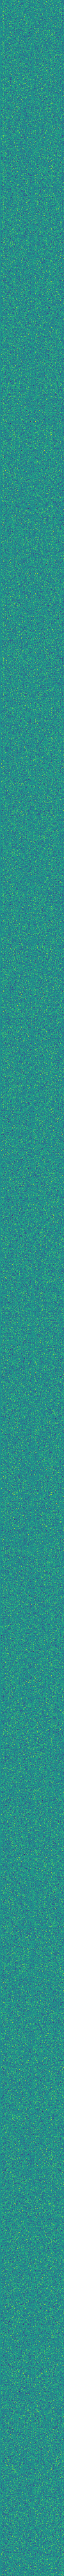
\includegraphics[interpolate=false,width=1.000000in,height=1.000000in]{antiderivative_ci_50-img0.png}}%
\end{pgfscope}%
\begin{pgfscope}%
\pgfsetbuttcap%
\pgfsetroundjoin%
\definecolor{currentfill}{rgb}{0.000000,0.000000,0.000000}%
\pgfsetfillcolor{currentfill}%
\pgfsetlinewidth{0.803000pt}%
\definecolor{currentstroke}{rgb}{0.000000,0.000000,0.000000}%
\pgfsetstrokecolor{currentstroke}%
\pgfsetdash{}{0pt}%
\pgfsys@defobject{currentmarker}{\pgfqpoint{0.000000in}{-0.048611in}}{\pgfqpoint{0.000000in}{0.000000in}}{%
\pgfpathmoveto{\pgfqpoint{0.000000in}{0.000000in}}%
\pgfpathlineto{\pgfqpoint{0.000000in}{-0.048611in}}%
\pgfusepath{stroke,fill}%
}%
\begin{pgfscope}%
\pgfsys@transformshift{0.800000in}{0.528000in}%
\pgfsys@useobject{currentmarker}{}%
\end{pgfscope}%
\end{pgfscope}%
\begin{pgfscope}%
\definecolor{textcolor}{rgb}{0.000000,0.000000,0.000000}%
\pgfsetstrokecolor{textcolor}%
\pgfsetfillcolor{textcolor}%
\pgftext[x=0.800000in,y=0.430778in,,top]{\color{textcolor}{\rmfamily\fontsize{12.000000}{14.400000}\selectfont\catcode`\^=\active\def^{\ifmmode\sp\else\^{}\fi}\catcode`\%=\active\def%{\%}0}}%
\end{pgfscope}%
\begin{pgfscope}%
\pgfsetbuttcap%
\pgfsetroundjoin%
\definecolor{currentfill}{rgb}{0.000000,0.000000,0.000000}%
\pgfsetfillcolor{currentfill}%
\pgfsetlinewidth{0.803000pt}%
\definecolor{currentstroke}{rgb}{0.000000,0.000000,0.000000}%
\pgfsetstrokecolor{currentstroke}%
\pgfsetdash{}{0pt}%
\pgfsys@defobject{currentmarker}{\pgfqpoint{0.000000in}{-0.048611in}}{\pgfqpoint{0.000000in}{0.000000in}}{%
\pgfpathmoveto{\pgfqpoint{0.000000in}{0.000000in}}%
\pgfpathlineto{\pgfqpoint{0.000000in}{-0.048611in}}%
\pgfusepath{stroke,fill}%
}%
\begin{pgfscope}%
\pgfsys@transformshift{1.593600in}{0.528000in}%
\pgfsys@useobject{currentmarker}{}%
\end{pgfscope}%
\end{pgfscope}%
\begin{pgfscope}%
\definecolor{textcolor}{rgb}{0.000000,0.000000,0.000000}%
\pgfsetstrokecolor{textcolor}%
\pgfsetfillcolor{textcolor}%
\pgftext[x=1.593600in,y=0.430778in,,top]{\color{textcolor}{\rmfamily\fontsize{12.000000}{14.400000}\selectfont\catcode`\^=\active\def^{\ifmmode\sp\else\^{}\fi}\catcode`\%=\active\def%{\%}10}}%
\end{pgfscope}%
\begin{pgfscope}%
\pgfsetbuttcap%
\pgfsetroundjoin%
\definecolor{currentfill}{rgb}{0.000000,0.000000,0.000000}%
\pgfsetfillcolor{currentfill}%
\pgfsetlinewidth{0.803000pt}%
\definecolor{currentstroke}{rgb}{0.000000,0.000000,0.000000}%
\pgfsetstrokecolor{currentstroke}%
\pgfsetdash{}{0pt}%
\pgfsys@defobject{currentmarker}{\pgfqpoint{0.000000in}{-0.048611in}}{\pgfqpoint{0.000000in}{0.000000in}}{%
\pgfpathmoveto{\pgfqpoint{0.000000in}{0.000000in}}%
\pgfpathlineto{\pgfqpoint{0.000000in}{-0.048611in}}%
\pgfusepath{stroke,fill}%
}%
\begin{pgfscope}%
\pgfsys@transformshift{2.387200in}{0.528000in}%
\pgfsys@useobject{currentmarker}{}%
\end{pgfscope}%
\end{pgfscope}%
\begin{pgfscope}%
\definecolor{textcolor}{rgb}{0.000000,0.000000,0.000000}%
\pgfsetstrokecolor{textcolor}%
\pgfsetfillcolor{textcolor}%
\pgftext[x=2.387200in,y=0.430778in,,top]{\color{textcolor}{\rmfamily\fontsize{12.000000}{14.400000}\selectfont\catcode`\^=\active\def^{\ifmmode\sp\else\^{}\fi}\catcode`\%=\active\def%{\%}20}}%
\end{pgfscope}%
\begin{pgfscope}%
\pgfsetbuttcap%
\pgfsetroundjoin%
\definecolor{currentfill}{rgb}{0.000000,0.000000,0.000000}%
\pgfsetfillcolor{currentfill}%
\pgfsetlinewidth{0.803000pt}%
\definecolor{currentstroke}{rgb}{0.000000,0.000000,0.000000}%
\pgfsetstrokecolor{currentstroke}%
\pgfsetdash{}{0pt}%
\pgfsys@defobject{currentmarker}{\pgfqpoint{0.000000in}{-0.048611in}}{\pgfqpoint{0.000000in}{0.000000in}}{%
\pgfpathmoveto{\pgfqpoint{0.000000in}{0.000000in}}%
\pgfpathlineto{\pgfqpoint{0.000000in}{-0.048611in}}%
\pgfusepath{stroke,fill}%
}%
\begin{pgfscope}%
\pgfsys@transformshift{3.180800in}{0.528000in}%
\pgfsys@useobject{currentmarker}{}%
\end{pgfscope}%
\end{pgfscope}%
\begin{pgfscope}%
\definecolor{textcolor}{rgb}{0.000000,0.000000,0.000000}%
\pgfsetstrokecolor{textcolor}%
\pgfsetfillcolor{textcolor}%
\pgftext[x=3.180800in,y=0.430778in,,top]{\color{textcolor}{\rmfamily\fontsize{12.000000}{14.400000}\selectfont\catcode`\^=\active\def^{\ifmmode\sp\else\^{}\fi}\catcode`\%=\active\def%{\%}30}}%
\end{pgfscope}%
\begin{pgfscope}%
\pgfsetbuttcap%
\pgfsetroundjoin%
\definecolor{currentfill}{rgb}{0.000000,0.000000,0.000000}%
\pgfsetfillcolor{currentfill}%
\pgfsetlinewidth{0.803000pt}%
\definecolor{currentstroke}{rgb}{0.000000,0.000000,0.000000}%
\pgfsetstrokecolor{currentstroke}%
\pgfsetdash{}{0pt}%
\pgfsys@defobject{currentmarker}{\pgfqpoint{0.000000in}{-0.048611in}}{\pgfqpoint{0.000000in}{0.000000in}}{%
\pgfpathmoveto{\pgfqpoint{0.000000in}{0.000000in}}%
\pgfpathlineto{\pgfqpoint{0.000000in}{-0.048611in}}%
\pgfusepath{stroke,fill}%
}%
\begin{pgfscope}%
\pgfsys@transformshift{3.974400in}{0.528000in}%
\pgfsys@useobject{currentmarker}{}%
\end{pgfscope}%
\end{pgfscope}%
\begin{pgfscope}%
\definecolor{textcolor}{rgb}{0.000000,0.000000,0.000000}%
\pgfsetstrokecolor{textcolor}%
\pgfsetfillcolor{textcolor}%
\pgftext[x=3.974400in,y=0.430778in,,top]{\color{textcolor}{\rmfamily\fontsize{12.000000}{14.400000}\selectfont\catcode`\^=\active\def^{\ifmmode\sp\else\^{}\fi}\catcode`\%=\active\def%{\%}40}}%
\end{pgfscope}%
\begin{pgfscope}%
\pgfsetbuttcap%
\pgfsetroundjoin%
\definecolor{currentfill}{rgb}{0.000000,0.000000,0.000000}%
\pgfsetfillcolor{currentfill}%
\pgfsetlinewidth{0.803000pt}%
\definecolor{currentstroke}{rgb}{0.000000,0.000000,0.000000}%
\pgfsetstrokecolor{currentstroke}%
\pgfsetdash{}{0pt}%
\pgfsys@defobject{currentmarker}{\pgfqpoint{0.000000in}{-0.048611in}}{\pgfqpoint{0.000000in}{0.000000in}}{%
\pgfpathmoveto{\pgfqpoint{0.000000in}{0.000000in}}%
\pgfpathlineto{\pgfqpoint{0.000000in}{-0.048611in}}%
\pgfusepath{stroke,fill}%
}%
\begin{pgfscope}%
\pgfsys@transformshift{4.768000in}{0.528000in}%
\pgfsys@useobject{currentmarker}{}%
\end{pgfscope}%
\end{pgfscope}%
\begin{pgfscope}%
\definecolor{textcolor}{rgb}{0.000000,0.000000,0.000000}%
\pgfsetstrokecolor{textcolor}%
\pgfsetfillcolor{textcolor}%
\pgftext[x=4.768000in,y=0.430778in,,top]{\color{textcolor}{\rmfamily\fontsize{12.000000}{14.400000}\selectfont\catcode`\^=\active\def^{\ifmmode\sp\else\^{}\fi}\catcode`\%=\active\def%{\%}50}}%
\end{pgfscope}%
\begin{pgfscope}%
\definecolor{textcolor}{rgb}{0.000000,0.000000,0.000000}%
\pgfsetstrokecolor{textcolor}%
\pgfsetfillcolor{textcolor}%
\pgftext[x=2.784000in,y=0.213927in,,top]{\color{textcolor}{\rmfamily\fontsize{12.000000}{14.400000}\selectfont\catcode`\^=\active\def^{\ifmmode\sp\else\^{}\fi}\catcode`\%=\active\def%{\%}input coefficients}}%
\end{pgfscope}%
\begin{pgfscope}%
\pgfsetbuttcap%
\pgfsetroundjoin%
\definecolor{currentfill}{rgb}{0.000000,0.000000,0.000000}%
\pgfsetfillcolor{currentfill}%
\pgfsetlinewidth{0.803000pt}%
\definecolor{currentstroke}{rgb}{0.000000,0.000000,0.000000}%
\pgfsetstrokecolor{currentstroke}%
\pgfsetdash{}{0pt}%
\pgfsys@defobject{currentmarker}{\pgfqpoint{-0.048611in}{0.000000in}}{\pgfqpoint{-0.000000in}{0.000000in}}{%
\pgfpathmoveto{\pgfqpoint{-0.000000in}{0.000000in}}%
\pgfpathlineto{\pgfqpoint{-0.048611in}{0.000000in}}%
\pgfusepath{stroke,fill}%
}%
\begin{pgfscope}%
\pgfsys@transformshift{0.800000in}{4.224000in}%
\pgfsys@useobject{currentmarker}{}%
\end{pgfscope}%
\end{pgfscope}%
\begin{pgfscope}%
\definecolor{textcolor}{rgb}{0.000000,0.000000,0.000000}%
\pgfsetstrokecolor{textcolor}%
\pgfsetfillcolor{textcolor}%
\pgftext[x=0.596739in, y=4.160686in, left, base]{\color{textcolor}{\rmfamily\fontsize{12.000000}{14.400000}\selectfont\catcode`\^=\active\def^{\ifmmode\sp\else\^{}\fi}\catcode`\%=\active\def%{\%}0}}%
\end{pgfscope}%
\begin{pgfscope}%
\pgfsetbuttcap%
\pgfsetroundjoin%
\definecolor{currentfill}{rgb}{0.000000,0.000000,0.000000}%
\pgfsetfillcolor{currentfill}%
\pgfsetlinewidth{0.803000pt}%
\definecolor{currentstroke}{rgb}{0.000000,0.000000,0.000000}%
\pgfsetstrokecolor{currentstroke}%
\pgfsetdash{}{0pt}%
\pgfsys@defobject{currentmarker}{\pgfqpoint{-0.048611in}{0.000000in}}{\pgfqpoint{-0.000000in}{0.000000in}}{%
\pgfpathmoveto{\pgfqpoint{-0.000000in}{0.000000in}}%
\pgfpathlineto{\pgfqpoint{-0.048611in}{0.000000in}}%
\pgfusepath{stroke,fill}%
}%
\begin{pgfscope}%
\pgfsys@transformshift{0.800000in}{3.762000in}%
\pgfsys@useobject{currentmarker}{}%
\end{pgfscope}%
\end{pgfscope}%
\begin{pgfscope}%
\definecolor{textcolor}{rgb}{0.000000,0.000000,0.000000}%
\pgfsetstrokecolor{textcolor}%
\pgfsetfillcolor{textcolor}%
\pgftext[x=0.384662in, y=3.698686in, left, base]{\color{textcolor}{\rmfamily\fontsize{12.000000}{14.400000}\selectfont\catcode`\^=\active\def^{\ifmmode\sp\else\^{}\fi}\catcode`\%=\active\def%{\%}500}}%
\end{pgfscope}%
\begin{pgfscope}%
\pgfsetbuttcap%
\pgfsetroundjoin%
\definecolor{currentfill}{rgb}{0.000000,0.000000,0.000000}%
\pgfsetfillcolor{currentfill}%
\pgfsetlinewidth{0.803000pt}%
\definecolor{currentstroke}{rgb}{0.000000,0.000000,0.000000}%
\pgfsetstrokecolor{currentstroke}%
\pgfsetdash{}{0pt}%
\pgfsys@defobject{currentmarker}{\pgfqpoint{-0.048611in}{0.000000in}}{\pgfqpoint{-0.000000in}{0.000000in}}{%
\pgfpathmoveto{\pgfqpoint{-0.000000in}{0.000000in}}%
\pgfpathlineto{\pgfqpoint{-0.048611in}{0.000000in}}%
\pgfusepath{stroke,fill}%
}%
\begin{pgfscope}%
\pgfsys@transformshift{0.800000in}{3.300000in}%
\pgfsys@useobject{currentmarker}{}%
\end{pgfscope}%
\end{pgfscope}%
\begin{pgfscope}%
\definecolor{textcolor}{rgb}{0.000000,0.000000,0.000000}%
\pgfsetstrokecolor{textcolor}%
\pgfsetfillcolor{textcolor}%
\pgftext[x=0.278624in, y=3.236686in, left, base]{\color{textcolor}{\rmfamily\fontsize{12.000000}{14.400000}\selectfont\catcode`\^=\active\def^{\ifmmode\sp\else\^{}\fi}\catcode`\%=\active\def%{\%}1000}}%
\end{pgfscope}%
\begin{pgfscope}%
\pgfsetbuttcap%
\pgfsetroundjoin%
\definecolor{currentfill}{rgb}{0.000000,0.000000,0.000000}%
\pgfsetfillcolor{currentfill}%
\pgfsetlinewidth{0.803000pt}%
\definecolor{currentstroke}{rgb}{0.000000,0.000000,0.000000}%
\pgfsetstrokecolor{currentstroke}%
\pgfsetdash{}{0pt}%
\pgfsys@defobject{currentmarker}{\pgfqpoint{-0.048611in}{0.000000in}}{\pgfqpoint{-0.000000in}{0.000000in}}{%
\pgfpathmoveto{\pgfqpoint{-0.000000in}{0.000000in}}%
\pgfpathlineto{\pgfqpoint{-0.048611in}{0.000000in}}%
\pgfusepath{stroke,fill}%
}%
\begin{pgfscope}%
\pgfsys@transformshift{0.800000in}{2.838000in}%
\pgfsys@useobject{currentmarker}{}%
\end{pgfscope}%
\end{pgfscope}%
\begin{pgfscope}%
\definecolor{textcolor}{rgb}{0.000000,0.000000,0.000000}%
\pgfsetstrokecolor{textcolor}%
\pgfsetfillcolor{textcolor}%
\pgftext[x=0.278624in, y=2.774686in, left, base]{\color{textcolor}{\rmfamily\fontsize{12.000000}{14.400000}\selectfont\catcode`\^=\active\def^{\ifmmode\sp\else\^{}\fi}\catcode`\%=\active\def%{\%}1500}}%
\end{pgfscope}%
\begin{pgfscope}%
\pgfsetbuttcap%
\pgfsetroundjoin%
\definecolor{currentfill}{rgb}{0.000000,0.000000,0.000000}%
\pgfsetfillcolor{currentfill}%
\pgfsetlinewidth{0.803000pt}%
\definecolor{currentstroke}{rgb}{0.000000,0.000000,0.000000}%
\pgfsetstrokecolor{currentstroke}%
\pgfsetdash{}{0pt}%
\pgfsys@defobject{currentmarker}{\pgfqpoint{-0.048611in}{0.000000in}}{\pgfqpoint{-0.000000in}{0.000000in}}{%
\pgfpathmoveto{\pgfqpoint{-0.000000in}{0.000000in}}%
\pgfpathlineto{\pgfqpoint{-0.048611in}{0.000000in}}%
\pgfusepath{stroke,fill}%
}%
\begin{pgfscope}%
\pgfsys@transformshift{0.800000in}{2.376000in}%
\pgfsys@useobject{currentmarker}{}%
\end{pgfscope}%
\end{pgfscope}%
\begin{pgfscope}%
\definecolor{textcolor}{rgb}{0.000000,0.000000,0.000000}%
\pgfsetstrokecolor{textcolor}%
\pgfsetfillcolor{textcolor}%
\pgftext[x=0.278624in, y=2.312686in, left, base]{\color{textcolor}{\rmfamily\fontsize{12.000000}{14.400000}\selectfont\catcode`\^=\active\def^{\ifmmode\sp\else\^{}\fi}\catcode`\%=\active\def%{\%}2000}}%
\end{pgfscope}%
\begin{pgfscope}%
\pgfsetbuttcap%
\pgfsetroundjoin%
\definecolor{currentfill}{rgb}{0.000000,0.000000,0.000000}%
\pgfsetfillcolor{currentfill}%
\pgfsetlinewidth{0.803000pt}%
\definecolor{currentstroke}{rgb}{0.000000,0.000000,0.000000}%
\pgfsetstrokecolor{currentstroke}%
\pgfsetdash{}{0pt}%
\pgfsys@defobject{currentmarker}{\pgfqpoint{-0.048611in}{0.000000in}}{\pgfqpoint{-0.000000in}{0.000000in}}{%
\pgfpathmoveto{\pgfqpoint{-0.000000in}{0.000000in}}%
\pgfpathlineto{\pgfqpoint{-0.048611in}{0.000000in}}%
\pgfusepath{stroke,fill}%
}%
\begin{pgfscope}%
\pgfsys@transformshift{0.800000in}{1.914000in}%
\pgfsys@useobject{currentmarker}{}%
\end{pgfscope}%
\end{pgfscope}%
\begin{pgfscope}%
\definecolor{textcolor}{rgb}{0.000000,0.000000,0.000000}%
\pgfsetstrokecolor{textcolor}%
\pgfsetfillcolor{textcolor}%
\pgftext[x=0.278624in, y=1.850686in, left, base]{\color{textcolor}{\rmfamily\fontsize{12.000000}{14.400000}\selectfont\catcode`\^=\active\def^{\ifmmode\sp\else\^{}\fi}\catcode`\%=\active\def%{\%}2500}}%
\end{pgfscope}%
\begin{pgfscope}%
\pgfsetbuttcap%
\pgfsetroundjoin%
\definecolor{currentfill}{rgb}{0.000000,0.000000,0.000000}%
\pgfsetfillcolor{currentfill}%
\pgfsetlinewidth{0.803000pt}%
\definecolor{currentstroke}{rgb}{0.000000,0.000000,0.000000}%
\pgfsetstrokecolor{currentstroke}%
\pgfsetdash{}{0pt}%
\pgfsys@defobject{currentmarker}{\pgfqpoint{-0.048611in}{0.000000in}}{\pgfqpoint{-0.000000in}{0.000000in}}{%
\pgfpathmoveto{\pgfqpoint{-0.000000in}{0.000000in}}%
\pgfpathlineto{\pgfqpoint{-0.048611in}{0.000000in}}%
\pgfusepath{stroke,fill}%
}%
\begin{pgfscope}%
\pgfsys@transformshift{0.800000in}{1.452000in}%
\pgfsys@useobject{currentmarker}{}%
\end{pgfscope}%
\end{pgfscope}%
\begin{pgfscope}%
\definecolor{textcolor}{rgb}{0.000000,0.000000,0.000000}%
\pgfsetstrokecolor{textcolor}%
\pgfsetfillcolor{textcolor}%
\pgftext[x=0.278624in, y=1.388686in, left, base]{\color{textcolor}{\rmfamily\fontsize{12.000000}{14.400000}\selectfont\catcode`\^=\active\def^{\ifmmode\sp\else\^{}\fi}\catcode`\%=\active\def%{\%}3000}}%
\end{pgfscope}%
\begin{pgfscope}%
\pgfsetbuttcap%
\pgfsetroundjoin%
\definecolor{currentfill}{rgb}{0.000000,0.000000,0.000000}%
\pgfsetfillcolor{currentfill}%
\pgfsetlinewidth{0.803000pt}%
\definecolor{currentstroke}{rgb}{0.000000,0.000000,0.000000}%
\pgfsetstrokecolor{currentstroke}%
\pgfsetdash{}{0pt}%
\pgfsys@defobject{currentmarker}{\pgfqpoint{-0.048611in}{0.000000in}}{\pgfqpoint{-0.000000in}{0.000000in}}{%
\pgfpathmoveto{\pgfqpoint{-0.000000in}{0.000000in}}%
\pgfpathlineto{\pgfqpoint{-0.048611in}{0.000000in}}%
\pgfusepath{stroke,fill}%
}%
\begin{pgfscope}%
\pgfsys@transformshift{0.800000in}{0.990000in}%
\pgfsys@useobject{currentmarker}{}%
\end{pgfscope}%
\end{pgfscope}%
\begin{pgfscope}%
\definecolor{textcolor}{rgb}{0.000000,0.000000,0.000000}%
\pgfsetstrokecolor{textcolor}%
\pgfsetfillcolor{textcolor}%
\pgftext[x=0.278624in, y=0.926686in, left, base]{\color{textcolor}{\rmfamily\fontsize{12.000000}{14.400000}\selectfont\catcode`\^=\active\def^{\ifmmode\sp\else\^{}\fi}\catcode`\%=\active\def%{\%}3500}}%
\end{pgfscope}%
\begin{pgfscope}%
\pgfsetbuttcap%
\pgfsetroundjoin%
\definecolor{currentfill}{rgb}{0.000000,0.000000,0.000000}%
\pgfsetfillcolor{currentfill}%
\pgfsetlinewidth{0.803000pt}%
\definecolor{currentstroke}{rgb}{0.000000,0.000000,0.000000}%
\pgfsetstrokecolor{currentstroke}%
\pgfsetdash{}{0pt}%
\pgfsys@defobject{currentmarker}{\pgfqpoint{-0.048611in}{0.000000in}}{\pgfqpoint{-0.000000in}{0.000000in}}{%
\pgfpathmoveto{\pgfqpoint{-0.000000in}{0.000000in}}%
\pgfpathlineto{\pgfqpoint{-0.048611in}{0.000000in}}%
\pgfusepath{stroke,fill}%
}%
\begin{pgfscope}%
\pgfsys@transformshift{0.800000in}{0.528000in}%
\pgfsys@useobject{currentmarker}{}%
\end{pgfscope}%
\end{pgfscope}%
\begin{pgfscope}%
\definecolor{textcolor}{rgb}{0.000000,0.000000,0.000000}%
\pgfsetstrokecolor{textcolor}%
\pgfsetfillcolor{textcolor}%
\pgftext[x=0.278624in, y=0.464686in, left, base]{\color{textcolor}{\rmfamily\fontsize{12.000000}{14.400000}\selectfont\catcode`\^=\active\def^{\ifmmode\sp\else\^{}\fi}\catcode`\%=\active\def%{\%}4000}}%
\end{pgfscope}%
\begin{pgfscope}%
\definecolor{textcolor}{rgb}{0.000000,0.000000,0.000000}%
\pgfsetstrokecolor{textcolor}%
\pgfsetfillcolor{textcolor}%
\pgftext[x=0.223069in,y=2.376000in,,bottom,rotate=90.000000]{\color{textcolor}{\rmfamily\fontsize{12.000000}{14.400000}\selectfont\catcode`\^=\active\def^{\ifmmode\sp\else\^{}\fi}\catcode`\%=\active\def%{\%}samples}}%
\end{pgfscope}%
\begin{pgfscope}%
\pgfsetrectcap%
\pgfsetmiterjoin%
\pgfsetlinewidth{0.803000pt}%
\definecolor{currentstroke}{rgb}{0.000000,0.000000,0.000000}%
\pgfsetstrokecolor{currentstroke}%
\pgfsetdash{}{0pt}%
\pgfpathmoveto{\pgfqpoint{0.800000in}{0.528000in}}%
\pgfpathlineto{\pgfqpoint{0.800000in}{4.224000in}}%
\pgfusepath{stroke}%
\end{pgfscope}%
\begin{pgfscope}%
\pgfsetrectcap%
\pgfsetmiterjoin%
\pgfsetlinewidth{0.803000pt}%
\definecolor{currentstroke}{rgb}{0.000000,0.000000,0.000000}%
\pgfsetstrokecolor{currentstroke}%
\pgfsetdash{}{0pt}%
\pgfpathmoveto{\pgfqpoint{4.768000in}{0.528000in}}%
\pgfpathlineto{\pgfqpoint{4.768000in}{4.224000in}}%
\pgfusepath{stroke}%
\end{pgfscope}%
\begin{pgfscope}%
\pgfsetrectcap%
\pgfsetmiterjoin%
\pgfsetlinewidth{0.803000pt}%
\definecolor{currentstroke}{rgb}{0.000000,0.000000,0.000000}%
\pgfsetstrokecolor{currentstroke}%
\pgfsetdash{}{0pt}%
\pgfpathmoveto{\pgfqpoint{0.800000in}{0.528000in}}%
\pgfpathlineto{\pgfqpoint{4.768000in}{0.528000in}}%
\pgfusepath{stroke}%
\end{pgfscope}%
\begin{pgfscope}%
\pgfsetrectcap%
\pgfsetmiterjoin%
\pgfsetlinewidth{0.803000pt}%
\definecolor{currentstroke}{rgb}{0.000000,0.000000,0.000000}%
\pgfsetstrokecolor{currentstroke}%
\pgfsetdash{}{0pt}%
\pgfpathmoveto{\pgfqpoint{0.800000in}{4.224000in}}%
\pgfpathlineto{\pgfqpoint{4.768000in}{4.224000in}}%
\pgfusepath{stroke}%
\end{pgfscope}%
\begin{pgfscope}%
\pgfsetbuttcap%
\pgfsetmiterjoin%
\pgfsetlinewidth{0.000000pt}%
\definecolor{currentstroke}{rgb}{0.000000,0.000000,0.000000}%
\pgfsetstrokecolor{currentstroke}%
\pgfsetstrokeopacity{0.000000}%
\pgfsetdash{}{0pt}%
\pgfpathmoveto{\pgfqpoint{5.016000in}{0.528000in}}%
\pgfpathlineto{\pgfqpoint{5.200800in}{0.528000in}}%
\pgfpathlineto{\pgfqpoint{5.200800in}{4.224000in}}%
\pgfpathlineto{\pgfqpoint{5.016000in}{4.224000in}}%
\pgfpathlineto{\pgfqpoint{5.016000in}{0.528000in}}%
\pgfpathclose%
\pgfusepath{}%
\end{pgfscope}%
\begin{pgfscope}%
\pgfsys@transformshift{5.020000in}{0.530000in}%
\pgftext[left,bottom]{
\includegraphics[interpolate=true,width=0.180000in,height=3.690000in]{antiderivative_ci_50-img1.png}}%
\end{pgfscope}%
\begin{pgfscope}%
\pgfsetbuttcap%
\pgfsetroundjoin%
\definecolor{currentfill}{rgb}{0.000000,0.000000,0.000000}%
\pgfsetfillcolor{currentfill}%
\pgfsetlinewidth{0.803000pt}%
\definecolor{currentstroke}{rgb}{0.000000,0.000000,0.000000}%
\pgfsetstrokecolor{currentstroke}%
\pgfsetdash{}{0pt}%
\pgfsys@defobject{currentmarker}{\pgfqpoint{0.000000in}{0.000000in}}{\pgfqpoint{0.048611in}{0.000000in}}{%
\pgfpathmoveto{\pgfqpoint{0.000000in}{0.000000in}}%
\pgfpathlineto{\pgfqpoint{0.048611in}{0.000000in}}%
\pgfusepath{stroke,fill}%
}%
\begin{pgfscope}%
\pgfsys@transformshift{5.200800in}{0.540424in}%
\pgfsys@useobject{currentmarker}{}%
\end{pgfscope}%
\end{pgfscope}%
\begin{pgfscope}%
\definecolor{textcolor}{rgb}{0.000000,0.000000,0.000000}%
\pgfsetstrokecolor{textcolor}%
\pgfsetfillcolor{textcolor}%
\pgftext[x=5.298022in, y=0.477110in, left, base]{\color{textcolor}{\rmfamily\fontsize{12.000000}{14.400000}\selectfont\catcode`\^=\active\def^{\ifmmode\sp\else\^{}\fi}\catcode`\%=\active\def%{\%}\ensuremath{-}100}}%
\end{pgfscope}%
\begin{pgfscope}%
\pgfsetbuttcap%
\pgfsetroundjoin%
\definecolor{currentfill}{rgb}{0.000000,0.000000,0.000000}%
\pgfsetfillcolor{currentfill}%
\pgfsetlinewidth{0.803000pt}%
\definecolor{currentstroke}{rgb}{0.000000,0.000000,0.000000}%
\pgfsetstrokecolor{currentstroke}%
\pgfsetdash{}{0pt}%
\pgfsys@defobject{currentmarker}{\pgfqpoint{0.000000in}{0.000000in}}{\pgfqpoint{0.048611in}{0.000000in}}{%
\pgfpathmoveto{\pgfqpoint{0.000000in}{0.000000in}}%
\pgfpathlineto{\pgfqpoint{0.048611in}{0.000000in}}%
\pgfusepath{stroke,fill}%
}%
\begin{pgfscope}%
\pgfsys@transformshift{5.200800in}{0.999318in}%
\pgfsys@useobject{currentmarker}{}%
\end{pgfscope}%
\end{pgfscope}%
\begin{pgfscope}%
\definecolor{textcolor}{rgb}{0.000000,0.000000,0.000000}%
\pgfsetstrokecolor{textcolor}%
\pgfsetfillcolor{textcolor}%
\pgftext[x=5.298022in, y=0.936004in, left, base]{\color{textcolor}{\rmfamily\fontsize{12.000000}{14.400000}\selectfont\catcode`\^=\active\def^{\ifmmode\sp\else\^{}\fi}\catcode`\%=\active\def%{\%}\ensuremath{-}75}}%
\end{pgfscope}%
\begin{pgfscope}%
\pgfsetbuttcap%
\pgfsetroundjoin%
\definecolor{currentfill}{rgb}{0.000000,0.000000,0.000000}%
\pgfsetfillcolor{currentfill}%
\pgfsetlinewidth{0.803000pt}%
\definecolor{currentstroke}{rgb}{0.000000,0.000000,0.000000}%
\pgfsetstrokecolor{currentstroke}%
\pgfsetdash{}{0pt}%
\pgfsys@defobject{currentmarker}{\pgfqpoint{0.000000in}{0.000000in}}{\pgfqpoint{0.048611in}{0.000000in}}{%
\pgfpathmoveto{\pgfqpoint{0.000000in}{0.000000in}}%
\pgfpathlineto{\pgfqpoint{0.048611in}{0.000000in}}%
\pgfusepath{stroke,fill}%
}%
\begin{pgfscope}%
\pgfsys@transformshift{5.200800in}{1.458212in}%
\pgfsys@useobject{currentmarker}{}%
\end{pgfscope}%
\end{pgfscope}%
\begin{pgfscope}%
\definecolor{textcolor}{rgb}{0.000000,0.000000,0.000000}%
\pgfsetstrokecolor{textcolor}%
\pgfsetfillcolor{textcolor}%
\pgftext[x=5.298022in, y=1.394898in, left, base]{\color{textcolor}{\rmfamily\fontsize{12.000000}{14.400000}\selectfont\catcode`\^=\active\def^{\ifmmode\sp\else\^{}\fi}\catcode`\%=\active\def%{\%}\ensuremath{-}50}}%
\end{pgfscope}%
\begin{pgfscope}%
\pgfsetbuttcap%
\pgfsetroundjoin%
\definecolor{currentfill}{rgb}{0.000000,0.000000,0.000000}%
\pgfsetfillcolor{currentfill}%
\pgfsetlinewidth{0.803000pt}%
\definecolor{currentstroke}{rgb}{0.000000,0.000000,0.000000}%
\pgfsetstrokecolor{currentstroke}%
\pgfsetdash{}{0pt}%
\pgfsys@defobject{currentmarker}{\pgfqpoint{0.000000in}{0.000000in}}{\pgfqpoint{0.048611in}{0.000000in}}{%
\pgfpathmoveto{\pgfqpoint{0.000000in}{0.000000in}}%
\pgfpathlineto{\pgfqpoint{0.048611in}{0.000000in}}%
\pgfusepath{stroke,fill}%
}%
\begin{pgfscope}%
\pgfsys@transformshift{5.200800in}{1.917106in}%
\pgfsys@useobject{currentmarker}{}%
\end{pgfscope}%
\end{pgfscope}%
\begin{pgfscope}%
\definecolor{textcolor}{rgb}{0.000000,0.000000,0.000000}%
\pgfsetstrokecolor{textcolor}%
\pgfsetfillcolor{textcolor}%
\pgftext[x=5.298022in, y=1.853792in, left, base]{\color{textcolor}{\rmfamily\fontsize{12.000000}{14.400000}\selectfont\catcode`\^=\active\def^{\ifmmode\sp\else\^{}\fi}\catcode`\%=\active\def%{\%}\ensuremath{-}25}}%
\end{pgfscope}%
\begin{pgfscope}%
\pgfsetbuttcap%
\pgfsetroundjoin%
\definecolor{currentfill}{rgb}{0.000000,0.000000,0.000000}%
\pgfsetfillcolor{currentfill}%
\pgfsetlinewidth{0.803000pt}%
\definecolor{currentstroke}{rgb}{0.000000,0.000000,0.000000}%
\pgfsetstrokecolor{currentstroke}%
\pgfsetdash{}{0pt}%
\pgfsys@defobject{currentmarker}{\pgfqpoint{0.000000in}{0.000000in}}{\pgfqpoint{0.048611in}{0.000000in}}{%
\pgfpathmoveto{\pgfqpoint{0.000000in}{0.000000in}}%
\pgfpathlineto{\pgfqpoint{0.048611in}{0.000000in}}%
\pgfusepath{stroke,fill}%
}%
\begin{pgfscope}%
\pgfsys@transformshift{5.200800in}{2.376000in}%
\pgfsys@useobject{currentmarker}{}%
\end{pgfscope}%
\end{pgfscope}%
\begin{pgfscope}%
\definecolor{textcolor}{rgb}{0.000000,0.000000,0.000000}%
\pgfsetstrokecolor{textcolor}%
\pgfsetfillcolor{textcolor}%
\pgftext[x=5.298022in, y=2.312686in, left, base]{\color{textcolor}{\rmfamily\fontsize{12.000000}{14.400000}\selectfont\catcode`\^=\active\def^{\ifmmode\sp\else\^{}\fi}\catcode`\%=\active\def%{\%}0}}%
\end{pgfscope}%
\begin{pgfscope}%
\pgfsetbuttcap%
\pgfsetroundjoin%
\definecolor{currentfill}{rgb}{0.000000,0.000000,0.000000}%
\pgfsetfillcolor{currentfill}%
\pgfsetlinewidth{0.803000pt}%
\definecolor{currentstroke}{rgb}{0.000000,0.000000,0.000000}%
\pgfsetstrokecolor{currentstroke}%
\pgfsetdash{}{0pt}%
\pgfsys@defobject{currentmarker}{\pgfqpoint{0.000000in}{0.000000in}}{\pgfqpoint{0.048611in}{0.000000in}}{%
\pgfpathmoveto{\pgfqpoint{0.000000in}{0.000000in}}%
\pgfpathlineto{\pgfqpoint{0.048611in}{0.000000in}}%
\pgfusepath{stroke,fill}%
}%
\begin{pgfscope}%
\pgfsys@transformshift{5.200800in}{2.834894in}%
\pgfsys@useobject{currentmarker}{}%
\end{pgfscope}%
\end{pgfscope}%
\begin{pgfscope}%
\definecolor{textcolor}{rgb}{0.000000,0.000000,0.000000}%
\pgfsetstrokecolor{textcolor}%
\pgfsetfillcolor{textcolor}%
\pgftext[x=5.298022in, y=2.771580in, left, base]{\color{textcolor}{\rmfamily\fontsize{12.000000}{14.400000}\selectfont\catcode`\^=\active\def^{\ifmmode\sp\else\^{}\fi}\catcode`\%=\active\def%{\%}25}}%
\end{pgfscope}%
\begin{pgfscope}%
\pgfsetbuttcap%
\pgfsetroundjoin%
\definecolor{currentfill}{rgb}{0.000000,0.000000,0.000000}%
\pgfsetfillcolor{currentfill}%
\pgfsetlinewidth{0.803000pt}%
\definecolor{currentstroke}{rgb}{0.000000,0.000000,0.000000}%
\pgfsetstrokecolor{currentstroke}%
\pgfsetdash{}{0pt}%
\pgfsys@defobject{currentmarker}{\pgfqpoint{0.000000in}{0.000000in}}{\pgfqpoint{0.048611in}{0.000000in}}{%
\pgfpathmoveto{\pgfqpoint{0.000000in}{0.000000in}}%
\pgfpathlineto{\pgfqpoint{0.048611in}{0.000000in}}%
\pgfusepath{stroke,fill}%
}%
\begin{pgfscope}%
\pgfsys@transformshift{5.200800in}{3.293788in}%
\pgfsys@useobject{currentmarker}{}%
\end{pgfscope}%
\end{pgfscope}%
\begin{pgfscope}%
\definecolor{textcolor}{rgb}{0.000000,0.000000,0.000000}%
\pgfsetstrokecolor{textcolor}%
\pgfsetfillcolor{textcolor}%
\pgftext[x=5.298022in, y=3.230474in, left, base]{\color{textcolor}{\rmfamily\fontsize{12.000000}{14.400000}\selectfont\catcode`\^=\active\def^{\ifmmode\sp\else\^{}\fi}\catcode`\%=\active\def%{\%}50}}%
\end{pgfscope}%
\begin{pgfscope}%
\pgfsetbuttcap%
\pgfsetroundjoin%
\definecolor{currentfill}{rgb}{0.000000,0.000000,0.000000}%
\pgfsetfillcolor{currentfill}%
\pgfsetlinewidth{0.803000pt}%
\definecolor{currentstroke}{rgb}{0.000000,0.000000,0.000000}%
\pgfsetstrokecolor{currentstroke}%
\pgfsetdash{}{0pt}%
\pgfsys@defobject{currentmarker}{\pgfqpoint{0.000000in}{0.000000in}}{\pgfqpoint{0.048611in}{0.000000in}}{%
\pgfpathmoveto{\pgfqpoint{0.000000in}{0.000000in}}%
\pgfpathlineto{\pgfqpoint{0.048611in}{0.000000in}}%
\pgfusepath{stroke,fill}%
}%
\begin{pgfscope}%
\pgfsys@transformshift{5.200800in}{3.752682in}%
\pgfsys@useobject{currentmarker}{}%
\end{pgfscope}%
\end{pgfscope}%
\begin{pgfscope}%
\definecolor{textcolor}{rgb}{0.000000,0.000000,0.000000}%
\pgfsetstrokecolor{textcolor}%
\pgfsetfillcolor{textcolor}%
\pgftext[x=5.298022in, y=3.689368in, left, base]{\color{textcolor}{\rmfamily\fontsize{12.000000}{14.400000}\selectfont\catcode`\^=\active\def^{\ifmmode\sp\else\^{}\fi}\catcode`\%=\active\def%{\%}75}}%
\end{pgfscope}%
\begin{pgfscope}%
\pgfsetbuttcap%
\pgfsetroundjoin%
\definecolor{currentfill}{rgb}{0.000000,0.000000,0.000000}%
\pgfsetfillcolor{currentfill}%
\pgfsetlinewidth{0.803000pt}%
\definecolor{currentstroke}{rgb}{0.000000,0.000000,0.000000}%
\pgfsetstrokecolor{currentstroke}%
\pgfsetdash{}{0pt}%
\pgfsys@defobject{currentmarker}{\pgfqpoint{0.000000in}{0.000000in}}{\pgfqpoint{0.048611in}{0.000000in}}{%
\pgfpathmoveto{\pgfqpoint{0.000000in}{0.000000in}}%
\pgfpathlineto{\pgfqpoint{0.048611in}{0.000000in}}%
\pgfusepath{stroke,fill}%
}%
\begin{pgfscope}%
\pgfsys@transformshift{5.200800in}{4.211576in}%
\pgfsys@useobject{currentmarker}{}%
\end{pgfscope}%
\end{pgfscope}%
\begin{pgfscope}%
\definecolor{textcolor}{rgb}{0.000000,0.000000,0.000000}%
\pgfsetstrokecolor{textcolor}%
\pgfsetfillcolor{textcolor}%
\pgftext[x=5.298022in, y=4.148262in, left, base]{\color{textcolor}{\rmfamily\fontsize{12.000000}{14.400000}\selectfont\catcode`\^=\active\def^{\ifmmode\sp\else\^{}\fi}\catcode`\%=\active\def%{\%}100}}%
\end{pgfscope}%
\begin{pgfscope}%
\pgfsetrectcap%
\pgfsetmiterjoin%
\pgfsetlinewidth{0.803000pt}%
\definecolor{currentstroke}{rgb}{0.000000,0.000000,0.000000}%
\pgfsetstrokecolor{currentstroke}%
\pgfsetdash{}{0pt}%
\pgfpathmoveto{\pgfqpoint{5.016000in}{0.528000in}}%
\pgfpathlineto{\pgfqpoint{5.108400in}{0.528000in}}%
\pgfpathlineto{\pgfqpoint{5.200800in}{0.528000in}}%
\pgfpathlineto{\pgfqpoint{5.200800in}{4.224000in}}%
\pgfpathlineto{\pgfqpoint{5.108400in}{4.224000in}}%
\pgfpathlineto{\pgfqpoint{5.016000in}{4.224000in}}%
\pgfpathlineto{\pgfqpoint{5.016000in}{0.528000in}}%
\pgfpathclose%
\pgfusepath{stroke}%
\end{pgfscope}%
\end{pgfpicture}%
\makeatother%
\endgroup%

    \end{adjustbox}
    \caption{Correlation image 50\% noise.}\label{fig:sc1_ci_50}
  \end{subfigure}
  \begin{subfigure}{0.49\linewidth}
    \begin{adjustbox}{width=1.2\linewidth}
      \begingroup%
\makeatletter%
\begin{pgfpicture}%
\pgfpathrectangle{\pgfpointorigin}{\pgfqpoint{4.000000in}{3.000000in}}%
\pgfusepath{use as bounding box, clip}%
\begin{pgfscope}%
\pgfsetbuttcap%
\pgfsetmiterjoin%
\pgfsetlinewidth{0.000000pt}%
\definecolor{currentstroke}{rgb}{0.000000,0.000000,0.000000}%
\pgfsetstrokecolor{currentstroke}%
\pgfsetstrokeopacity{0.000000}%
\pgfsetdash{}{0pt}%
\pgfpathmoveto{\pgfqpoint{0.000000in}{0.000000in}}%
\pgfpathlineto{\pgfqpoint{4.000000in}{0.000000in}}%
\pgfpathlineto{\pgfqpoint{4.000000in}{3.000000in}}%
\pgfpathlineto{\pgfqpoint{0.000000in}{3.000000in}}%
\pgfpathlineto{\pgfqpoint{0.000000in}{0.000000in}}%
\pgfpathclose%
\pgfusepath{}%
\end{pgfscope}%
\begin{pgfscope}%
\pgfsetbuttcap%
\pgfsetmiterjoin%
\pgfsetlinewidth{0.000000pt}%
\definecolor{currentstroke}{rgb}{0.000000,0.000000,0.000000}%
\pgfsetstrokecolor{currentstroke}%
\pgfsetstrokeopacity{0.000000}%
\pgfsetdash{}{0pt}%
\pgfpathmoveto{\pgfqpoint{0.642156in}{0.517039in}}%
\pgfpathlineto{\pgfqpoint{3.032083in}{0.517039in}}%
\pgfpathlineto{\pgfqpoint{3.032083in}{2.906966in}}%
\pgfpathlineto{\pgfqpoint{0.642156in}{2.906966in}}%
\pgfpathlineto{\pgfqpoint{0.642156in}{0.517039in}}%
\pgfpathclose%
\pgfusepath{}%
\end{pgfscope}%
\begin{pgfscope}%
\pgfpathrectangle{\pgfqpoint{0.642156in}{0.517039in}}{\pgfqpoint{2.389927in}{2.389927in}}%
\pgfusepath{clip}%
\pgfsys@transformcm{2.389927}{0.000000}{0.000000}{-2.389927}{0.642156in}{2.906966in}%
\pgftext[left,bottom]{
\includegraphics[interpolate=false,width=1.000000in,height=1.000000in]{antiderivative_pm_50-img0.png}}%
\end{pgfscope}%
\begin{pgfscope}%
\pgfsetbuttcap%
\pgfsetroundjoin%
\definecolor{currentfill}{rgb}{0.000000,0.000000,0.000000}%
\pgfsetfillcolor{currentfill}%
\pgfsetlinewidth{0.803000pt}%
\definecolor{currentstroke}{rgb}{0.000000,0.000000,0.000000}%
\pgfsetstrokecolor{currentstroke}%
\pgfsetdash{}{0pt}%
\pgfsys@defobject{currentmarker}{\pgfqpoint{0.000000in}{-0.048611in}}{\pgfqpoint{0.000000in}{0.000000in}}{%
\pgfpathmoveto{\pgfqpoint{0.000000in}{0.000000in}}%
\pgfpathlineto{\pgfqpoint{0.000000in}{-0.048611in}}%
\pgfusepath{stroke,fill}%
}%
\begin{pgfscope}%
\pgfsys@transformshift{0.654106in}{0.517039in}%
\pgfsys@useobject{currentmarker}{}%
\end{pgfscope}%
\end{pgfscope}%
\begin{pgfscope}%
\definecolor{textcolor}{rgb}{0.000000,0.000000,0.000000}%
\pgfsetstrokecolor{textcolor}%
\pgfsetfillcolor{textcolor}%
\pgftext[x=0.654106in,y=0.419816in,,top]{\color{textcolor}{\rmfamily\fontsize{12.000000}{14.400000}\selectfont\catcode`\^=\active\def^{\ifmmode\sp\else\^{}\fi}\catcode`\%=\active\def%{\%}0}}%
\end{pgfscope}%
\begin{pgfscope}%
\pgfsetbuttcap%
\pgfsetroundjoin%
\definecolor{currentfill}{rgb}{0.000000,0.000000,0.000000}%
\pgfsetfillcolor{currentfill}%
\pgfsetlinewidth{0.803000pt}%
\definecolor{currentstroke}{rgb}{0.000000,0.000000,0.000000}%
\pgfsetstrokecolor{currentstroke}%
\pgfsetdash{}{0pt}%
\pgfsys@defobject{currentmarker}{\pgfqpoint{0.000000in}{-0.048611in}}{\pgfqpoint{0.000000in}{0.000000in}}{%
\pgfpathmoveto{\pgfqpoint{0.000000in}{0.000000in}}%
\pgfpathlineto{\pgfqpoint{0.000000in}{-0.048611in}}%
\pgfusepath{stroke,fill}%
}%
\begin{pgfscope}%
\pgfsys@transformshift{1.251588in}{0.517039in}%
\pgfsys@useobject{currentmarker}{}%
\end{pgfscope}%
\end{pgfscope}%
\begin{pgfscope}%
\definecolor{textcolor}{rgb}{0.000000,0.000000,0.000000}%
\pgfsetstrokecolor{textcolor}%
\pgfsetfillcolor{textcolor}%
\pgftext[x=1.251588in,y=0.419816in,,top]{\color{textcolor}{\rmfamily\fontsize{12.000000}{14.400000}\selectfont\catcode`\^=\active\def^{\ifmmode\sp\else\^{}\fi}\catcode`\%=\active\def%{\%}25}}%
\end{pgfscope}%
\begin{pgfscope}%
\pgfsetbuttcap%
\pgfsetroundjoin%
\definecolor{currentfill}{rgb}{0.000000,0.000000,0.000000}%
\pgfsetfillcolor{currentfill}%
\pgfsetlinewidth{0.803000pt}%
\definecolor{currentstroke}{rgb}{0.000000,0.000000,0.000000}%
\pgfsetstrokecolor{currentstroke}%
\pgfsetdash{}{0pt}%
\pgfsys@defobject{currentmarker}{\pgfqpoint{0.000000in}{-0.048611in}}{\pgfqpoint{0.000000in}{0.000000in}}{%
\pgfpathmoveto{\pgfqpoint{0.000000in}{0.000000in}}%
\pgfpathlineto{\pgfqpoint{0.000000in}{-0.048611in}}%
\pgfusepath{stroke,fill}%
}%
\begin{pgfscope}%
\pgfsys@transformshift{1.849069in}{0.517039in}%
\pgfsys@useobject{currentmarker}{}%
\end{pgfscope}%
\end{pgfscope}%
\begin{pgfscope}%
\definecolor{textcolor}{rgb}{0.000000,0.000000,0.000000}%
\pgfsetstrokecolor{textcolor}%
\pgfsetfillcolor{textcolor}%
\pgftext[x=1.849069in,y=0.419816in,,top]{\color{textcolor}{\rmfamily\fontsize{12.000000}{14.400000}\selectfont\catcode`\^=\active\def^{\ifmmode\sp\else\^{}\fi}\catcode`\%=\active\def%{\%}50}}%
\end{pgfscope}%
\begin{pgfscope}%
\pgfsetbuttcap%
\pgfsetroundjoin%
\definecolor{currentfill}{rgb}{0.000000,0.000000,0.000000}%
\pgfsetfillcolor{currentfill}%
\pgfsetlinewidth{0.803000pt}%
\definecolor{currentstroke}{rgb}{0.000000,0.000000,0.000000}%
\pgfsetstrokecolor{currentstroke}%
\pgfsetdash{}{0pt}%
\pgfsys@defobject{currentmarker}{\pgfqpoint{0.000000in}{-0.048611in}}{\pgfqpoint{0.000000in}{0.000000in}}{%
\pgfpathmoveto{\pgfqpoint{0.000000in}{0.000000in}}%
\pgfpathlineto{\pgfqpoint{0.000000in}{-0.048611in}}%
\pgfusepath{stroke,fill}%
}%
\begin{pgfscope}%
\pgfsys@transformshift{2.446551in}{0.517039in}%
\pgfsys@useobject{currentmarker}{}%
\end{pgfscope}%
\end{pgfscope}%
\begin{pgfscope}%
\definecolor{textcolor}{rgb}{0.000000,0.000000,0.000000}%
\pgfsetstrokecolor{textcolor}%
\pgfsetfillcolor{textcolor}%
\pgftext[x=2.446551in,y=0.419816in,,top]{\color{textcolor}{\rmfamily\fontsize{12.000000}{14.400000}\selectfont\catcode`\^=\active\def^{\ifmmode\sp\else\^{}\fi}\catcode`\%=\active\def%{\%}75}}%
\end{pgfscope}%
\begin{pgfscope}%
\definecolor{textcolor}{rgb}{0.000000,0.000000,0.000000}%
\pgfsetstrokecolor{textcolor}%
\pgfsetfillcolor{textcolor}%
\pgftext[x=1.837120in,y=0.202965in,,top]{\color{textcolor}{\rmfamily\fontsize{12.000000}{14.400000}\selectfont\catcode`\^=\active\def^{\ifmmode\sp\else\^{}\fi}\catcode`\%=\active\def%{\%}output coefficients}}%
\end{pgfscope}%
\begin{pgfscope}%
\pgfsetbuttcap%
\pgfsetroundjoin%
\definecolor{currentfill}{rgb}{0.000000,0.000000,0.000000}%
\pgfsetfillcolor{currentfill}%
\pgfsetlinewidth{0.803000pt}%
\definecolor{currentstroke}{rgb}{0.000000,0.000000,0.000000}%
\pgfsetstrokecolor{currentstroke}%
\pgfsetdash{}{0pt}%
\pgfsys@defobject{currentmarker}{\pgfqpoint{-0.048611in}{0.000000in}}{\pgfqpoint{-0.000000in}{0.000000in}}{%
\pgfpathmoveto{\pgfqpoint{-0.000000in}{0.000000in}}%
\pgfpathlineto{\pgfqpoint{-0.048611in}{0.000000in}}%
\pgfusepath{stroke,fill}%
}%
\begin{pgfscope}%
\pgfsys@transformshift{0.642156in}{2.895016in}%
\pgfsys@useobject{currentmarker}{}%
\end{pgfscope}%
\end{pgfscope}%
\begin{pgfscope}%
\definecolor{textcolor}{rgb}{0.000000,0.000000,0.000000}%
\pgfsetstrokecolor{textcolor}%
\pgfsetfillcolor{textcolor}%
\pgftext[x=0.438896in, y=2.831702in, left, base]{\color{textcolor}{\rmfamily\fontsize{12.000000}{14.400000}\selectfont\catcode`\^=\active\def^{\ifmmode\sp\else\^{}\fi}\catcode`\%=\active\def%{\%}0}}%
\end{pgfscope}%
\begin{pgfscope}%
\pgfsetbuttcap%
\pgfsetroundjoin%
\definecolor{currentfill}{rgb}{0.000000,0.000000,0.000000}%
\pgfsetfillcolor{currentfill}%
\pgfsetlinewidth{0.803000pt}%
\definecolor{currentstroke}{rgb}{0.000000,0.000000,0.000000}%
\pgfsetstrokecolor{currentstroke}%
\pgfsetdash{}{0pt}%
\pgfsys@defobject{currentmarker}{\pgfqpoint{-0.048611in}{0.000000in}}{\pgfqpoint{-0.000000in}{0.000000in}}{%
\pgfpathmoveto{\pgfqpoint{-0.000000in}{0.000000in}}%
\pgfpathlineto{\pgfqpoint{-0.048611in}{0.000000in}}%
\pgfusepath{stroke,fill}%
}%
\begin{pgfscope}%
\pgfsys@transformshift{0.642156in}{2.417031in}%
\pgfsys@useobject{currentmarker}{}%
\end{pgfscope}%
\end{pgfscope}%
\begin{pgfscope}%
\definecolor{textcolor}{rgb}{0.000000,0.000000,0.000000}%
\pgfsetstrokecolor{textcolor}%
\pgfsetfillcolor{textcolor}%
\pgftext[x=0.332857in, y=2.353717in, left, base]{\color{textcolor}{\rmfamily\fontsize{12.000000}{14.400000}\selectfont\catcode`\^=\active\def^{\ifmmode\sp\else\^{}\fi}\catcode`\%=\active\def%{\%}20}}%
\end{pgfscope}%
\begin{pgfscope}%
\pgfsetbuttcap%
\pgfsetroundjoin%
\definecolor{currentfill}{rgb}{0.000000,0.000000,0.000000}%
\pgfsetfillcolor{currentfill}%
\pgfsetlinewidth{0.803000pt}%
\definecolor{currentstroke}{rgb}{0.000000,0.000000,0.000000}%
\pgfsetstrokecolor{currentstroke}%
\pgfsetdash{}{0pt}%
\pgfsys@defobject{currentmarker}{\pgfqpoint{-0.048611in}{0.000000in}}{\pgfqpoint{-0.000000in}{0.000000in}}{%
\pgfpathmoveto{\pgfqpoint{-0.000000in}{0.000000in}}%
\pgfpathlineto{\pgfqpoint{-0.048611in}{0.000000in}}%
\pgfusepath{stroke,fill}%
}%
\begin{pgfscope}%
\pgfsys@transformshift{0.642156in}{1.939045in}%
\pgfsys@useobject{currentmarker}{}%
\end{pgfscope}%
\end{pgfscope}%
\begin{pgfscope}%
\definecolor{textcolor}{rgb}{0.000000,0.000000,0.000000}%
\pgfsetstrokecolor{textcolor}%
\pgfsetfillcolor{textcolor}%
\pgftext[x=0.332857in, y=1.875731in, left, base]{\color{textcolor}{\rmfamily\fontsize{12.000000}{14.400000}\selectfont\catcode`\^=\active\def^{\ifmmode\sp\else\^{}\fi}\catcode`\%=\active\def%{\%}40}}%
\end{pgfscope}%
\begin{pgfscope}%
\pgfsetbuttcap%
\pgfsetroundjoin%
\definecolor{currentfill}{rgb}{0.000000,0.000000,0.000000}%
\pgfsetfillcolor{currentfill}%
\pgfsetlinewidth{0.803000pt}%
\definecolor{currentstroke}{rgb}{0.000000,0.000000,0.000000}%
\pgfsetstrokecolor{currentstroke}%
\pgfsetdash{}{0pt}%
\pgfsys@defobject{currentmarker}{\pgfqpoint{-0.048611in}{0.000000in}}{\pgfqpoint{-0.000000in}{0.000000in}}{%
\pgfpathmoveto{\pgfqpoint{-0.000000in}{0.000000in}}%
\pgfpathlineto{\pgfqpoint{-0.048611in}{0.000000in}}%
\pgfusepath{stroke,fill}%
}%
\begin{pgfscope}%
\pgfsys@transformshift{0.642156in}{1.461060in}%
\pgfsys@useobject{currentmarker}{}%
\end{pgfscope}%
\end{pgfscope}%
\begin{pgfscope}%
\definecolor{textcolor}{rgb}{0.000000,0.000000,0.000000}%
\pgfsetstrokecolor{textcolor}%
\pgfsetfillcolor{textcolor}%
\pgftext[x=0.332857in, y=1.397746in, left, base]{\color{textcolor}{\rmfamily\fontsize{12.000000}{14.400000}\selectfont\catcode`\^=\active\def^{\ifmmode\sp\else\^{}\fi}\catcode`\%=\active\def%{\%}60}}%
\end{pgfscope}%
\begin{pgfscope}%
\pgfsetbuttcap%
\pgfsetroundjoin%
\definecolor{currentfill}{rgb}{0.000000,0.000000,0.000000}%
\pgfsetfillcolor{currentfill}%
\pgfsetlinewidth{0.803000pt}%
\definecolor{currentstroke}{rgb}{0.000000,0.000000,0.000000}%
\pgfsetstrokecolor{currentstroke}%
\pgfsetdash{}{0pt}%
\pgfsys@defobject{currentmarker}{\pgfqpoint{-0.048611in}{0.000000in}}{\pgfqpoint{-0.000000in}{0.000000in}}{%
\pgfpathmoveto{\pgfqpoint{-0.000000in}{0.000000in}}%
\pgfpathlineto{\pgfqpoint{-0.048611in}{0.000000in}}%
\pgfusepath{stroke,fill}%
}%
\begin{pgfscope}%
\pgfsys@transformshift{0.642156in}{0.983074in}%
\pgfsys@useobject{currentmarker}{}%
\end{pgfscope}%
\end{pgfscope}%
\begin{pgfscope}%
\definecolor{textcolor}{rgb}{0.000000,0.000000,0.000000}%
\pgfsetstrokecolor{textcolor}%
\pgfsetfillcolor{textcolor}%
\pgftext[x=0.332857in, y=0.919761in, left, base]{\color{textcolor}{\rmfamily\fontsize{12.000000}{14.400000}\selectfont\catcode`\^=\active\def^{\ifmmode\sp\else\^{}\fi}\catcode`\%=\active\def%{\%}80}}%
\end{pgfscope}%
\begin{pgfscope}%
\definecolor{textcolor}{rgb}{0.000000,0.000000,0.000000}%
\pgfsetstrokecolor{textcolor}%
\pgfsetfillcolor{textcolor}%
\pgftext[x=0.277302in,y=1.712002in,,bottom,rotate=90.000000]{\color{textcolor}{\rmfamily\fontsize{12.000000}{14.400000}\selectfont\catcode`\^=\active\def^{\ifmmode\sp\else\^{}\fi}\catcode`\%=\active\def%{\%}input coefficients}}%
\end{pgfscope}%
\begin{pgfscope}%
\pgfsetrectcap%
\pgfsetmiterjoin%
\pgfsetlinewidth{0.803000pt}%
\definecolor{currentstroke}{rgb}{0.000000,0.000000,0.000000}%
\pgfsetstrokecolor{currentstroke}%
\pgfsetdash{}{0pt}%
\pgfpathmoveto{\pgfqpoint{0.642156in}{0.517039in}}%
\pgfpathlineto{\pgfqpoint{0.642156in}{2.906966in}}%
\pgfusepath{stroke}%
\end{pgfscope}%
\begin{pgfscope}%
\pgfsetrectcap%
\pgfsetmiterjoin%
\pgfsetlinewidth{0.803000pt}%
\definecolor{currentstroke}{rgb}{0.000000,0.000000,0.000000}%
\pgfsetstrokecolor{currentstroke}%
\pgfsetdash{}{0pt}%
\pgfpathmoveto{\pgfqpoint{3.032083in}{0.517039in}}%
\pgfpathlineto{\pgfqpoint{3.032083in}{2.906966in}}%
\pgfusepath{stroke}%
\end{pgfscope}%
\begin{pgfscope}%
\pgfsetrectcap%
\pgfsetmiterjoin%
\pgfsetlinewidth{0.803000pt}%
\definecolor{currentstroke}{rgb}{0.000000,0.000000,0.000000}%
\pgfsetstrokecolor{currentstroke}%
\pgfsetdash{}{0pt}%
\pgfpathmoveto{\pgfqpoint{0.642156in}{0.517039in}}%
\pgfpathlineto{\pgfqpoint{3.032083in}{0.517039in}}%
\pgfusepath{stroke}%
\end{pgfscope}%
\begin{pgfscope}%
\pgfsetrectcap%
\pgfsetmiterjoin%
\pgfsetlinewidth{0.803000pt}%
\definecolor{currentstroke}{rgb}{0.000000,0.000000,0.000000}%
\pgfsetstrokecolor{currentstroke}%
\pgfsetdash{}{0pt}%
\pgfpathmoveto{\pgfqpoint{0.642156in}{2.906966in}}%
\pgfpathlineto{\pgfqpoint{3.032083in}{2.906966in}}%
\pgfusepath{stroke}%
\end{pgfscope}%
\begin{pgfscope}%
\pgfsetbuttcap%
\pgfsetmiterjoin%
\pgfsetlinewidth{0.000000pt}%
\definecolor{currentstroke}{rgb}{0.000000,0.000000,0.000000}%
\pgfsetstrokecolor{currentstroke}%
\pgfsetstrokeopacity{0.000000}%
\pgfsetdash{}{0pt}%
\pgfpathmoveto{\pgfqpoint{3.181604in}{0.517039in}}%
\pgfpathlineto{\pgfqpoint{3.301100in}{0.517039in}}%
\pgfpathlineto{\pgfqpoint{3.301100in}{2.906966in}}%
\pgfpathlineto{\pgfqpoint{3.181604in}{2.906966in}}%
\pgfpathlineto{\pgfqpoint{3.181604in}{0.517039in}}%
\pgfpathclose%
\pgfusepath{}%
\end{pgfscope}%
\begin{pgfscope}%
\pgfsys@transformshift{3.180000in}{0.520000in}%
\pgftext[left,bottom]{
\includegraphics[interpolate=true,width=0.120000in,height=2.390000in]{antiderivative_pm_50-img1.png}}%
\end{pgfscope}%
\begin{pgfscope}%
\pgfsetbuttcap%
\pgfsetroundjoin%
\definecolor{currentfill}{rgb}{0.000000,0.000000,0.000000}%
\pgfsetfillcolor{currentfill}%
\pgfsetlinewidth{0.803000pt}%
\definecolor{currentstroke}{rgb}{0.000000,0.000000,0.000000}%
\pgfsetstrokecolor{currentstroke}%
\pgfsetdash{}{0pt}%
\pgfsys@defobject{currentmarker}{\pgfqpoint{0.000000in}{0.000000in}}{\pgfqpoint{0.048611in}{0.000000in}}{%
\pgfpathmoveto{\pgfqpoint{0.000000in}{0.000000in}}%
\pgfpathlineto{\pgfqpoint{0.048611in}{0.000000in}}%
\pgfusepath{stroke,fill}%
}%
\begin{pgfscope}%
\pgfsys@transformshift{3.301100in}{0.707209in}%
\pgfsys@useobject{currentmarker}{}%
\end{pgfscope}%
\end{pgfscope}%
\begin{pgfscope}%
\definecolor{textcolor}{rgb}{0.000000,0.000000,0.000000}%
\pgfsetstrokecolor{textcolor}%
\pgfsetfillcolor{textcolor}%
\pgftext[x=3.398323in, y=0.643895in, left, base]{\color{textcolor}{\rmfamily\fontsize{12.000000}{14.400000}\selectfont\catcode`\^=\active\def^{\ifmmode\sp\else\^{}\fi}\catcode`\%=\active\def%{\%}\ensuremath{-}2000}}%
\end{pgfscope}%
\begin{pgfscope}%
\pgfsetbuttcap%
\pgfsetroundjoin%
\definecolor{currentfill}{rgb}{0.000000,0.000000,0.000000}%
\pgfsetfillcolor{currentfill}%
\pgfsetlinewidth{0.803000pt}%
\definecolor{currentstroke}{rgb}{0.000000,0.000000,0.000000}%
\pgfsetstrokecolor{currentstroke}%
\pgfsetdash{}{0pt}%
\pgfsys@defobject{currentmarker}{\pgfqpoint{0.000000in}{0.000000in}}{\pgfqpoint{0.048611in}{0.000000in}}{%
\pgfpathmoveto{\pgfqpoint{0.000000in}{0.000000in}}%
\pgfpathlineto{\pgfqpoint{0.048611in}{0.000000in}}%
\pgfusepath{stroke,fill}%
}%
\begin{pgfscope}%
\pgfsys@transformshift{3.301100in}{1.096875in}%
\pgfsys@useobject{currentmarker}{}%
\end{pgfscope}%
\end{pgfscope}%
\begin{pgfscope}%
\definecolor{textcolor}{rgb}{0.000000,0.000000,0.000000}%
\pgfsetstrokecolor{textcolor}%
\pgfsetfillcolor{textcolor}%
\pgftext[x=3.398323in, y=1.033561in, left, base]{\color{textcolor}{\rmfamily\fontsize{12.000000}{14.400000}\selectfont\catcode`\^=\active\def^{\ifmmode\sp\else\^{}\fi}\catcode`\%=\active\def%{\%}\ensuremath{-}1500}}%
\end{pgfscope}%
\begin{pgfscope}%
\pgfsetbuttcap%
\pgfsetroundjoin%
\definecolor{currentfill}{rgb}{0.000000,0.000000,0.000000}%
\pgfsetfillcolor{currentfill}%
\pgfsetlinewidth{0.803000pt}%
\definecolor{currentstroke}{rgb}{0.000000,0.000000,0.000000}%
\pgfsetstrokecolor{currentstroke}%
\pgfsetdash{}{0pt}%
\pgfsys@defobject{currentmarker}{\pgfqpoint{0.000000in}{0.000000in}}{\pgfqpoint{0.048611in}{0.000000in}}{%
\pgfpathmoveto{\pgfqpoint{0.000000in}{0.000000in}}%
\pgfpathlineto{\pgfqpoint{0.048611in}{0.000000in}}%
\pgfusepath{stroke,fill}%
}%
\begin{pgfscope}%
\pgfsys@transformshift{3.301100in}{1.486541in}%
\pgfsys@useobject{currentmarker}{}%
\end{pgfscope}%
\end{pgfscope}%
\begin{pgfscope}%
\definecolor{textcolor}{rgb}{0.000000,0.000000,0.000000}%
\pgfsetstrokecolor{textcolor}%
\pgfsetfillcolor{textcolor}%
\pgftext[x=3.398323in, y=1.423227in, left, base]{\color{textcolor}{\rmfamily\fontsize{12.000000}{14.400000}\selectfont\catcode`\^=\active\def^{\ifmmode\sp\else\^{}\fi}\catcode`\%=\active\def%{\%}\ensuremath{-}1000}}%
\end{pgfscope}%
\begin{pgfscope}%
\pgfsetbuttcap%
\pgfsetroundjoin%
\definecolor{currentfill}{rgb}{0.000000,0.000000,0.000000}%
\pgfsetfillcolor{currentfill}%
\pgfsetlinewidth{0.803000pt}%
\definecolor{currentstroke}{rgb}{0.000000,0.000000,0.000000}%
\pgfsetstrokecolor{currentstroke}%
\pgfsetdash{}{0pt}%
\pgfsys@defobject{currentmarker}{\pgfqpoint{0.000000in}{0.000000in}}{\pgfqpoint{0.048611in}{0.000000in}}{%
\pgfpathmoveto{\pgfqpoint{0.000000in}{0.000000in}}%
\pgfpathlineto{\pgfqpoint{0.048611in}{0.000000in}}%
\pgfusepath{stroke,fill}%
}%
\begin{pgfscope}%
\pgfsys@transformshift{3.301100in}{1.876208in}%
\pgfsys@useobject{currentmarker}{}%
\end{pgfscope}%
\end{pgfscope}%
\begin{pgfscope}%
\definecolor{textcolor}{rgb}{0.000000,0.000000,0.000000}%
\pgfsetstrokecolor{textcolor}%
\pgfsetfillcolor{textcolor}%
\pgftext[x=3.398323in, y=1.812894in, left, base]{\color{textcolor}{\rmfamily\fontsize{12.000000}{14.400000}\selectfont\catcode`\^=\active\def^{\ifmmode\sp\else\^{}\fi}\catcode`\%=\active\def%{\%}\ensuremath{-}500}}%
\end{pgfscope}%
\begin{pgfscope}%
\pgfsetbuttcap%
\pgfsetroundjoin%
\definecolor{currentfill}{rgb}{0.000000,0.000000,0.000000}%
\pgfsetfillcolor{currentfill}%
\pgfsetlinewidth{0.803000pt}%
\definecolor{currentstroke}{rgb}{0.000000,0.000000,0.000000}%
\pgfsetstrokecolor{currentstroke}%
\pgfsetdash{}{0pt}%
\pgfsys@defobject{currentmarker}{\pgfqpoint{0.000000in}{0.000000in}}{\pgfqpoint{0.048611in}{0.000000in}}{%
\pgfpathmoveto{\pgfqpoint{0.000000in}{0.000000in}}%
\pgfpathlineto{\pgfqpoint{0.048611in}{0.000000in}}%
\pgfusepath{stroke,fill}%
}%
\begin{pgfscope}%
\pgfsys@transformshift{3.301100in}{2.265874in}%
\pgfsys@useobject{currentmarker}{}%
\end{pgfscope}%
\end{pgfscope}%
\begin{pgfscope}%
\definecolor{textcolor}{rgb}{0.000000,0.000000,0.000000}%
\pgfsetstrokecolor{textcolor}%
\pgfsetfillcolor{textcolor}%
\pgftext[x=3.398323in, y=2.202560in, left, base]{\color{textcolor}{\rmfamily\fontsize{12.000000}{14.400000}\selectfont\catcode`\^=\active\def^{\ifmmode\sp\else\^{}\fi}\catcode`\%=\active\def%{\%}0}}%
\end{pgfscope}%
\begin{pgfscope}%
\pgfsetbuttcap%
\pgfsetroundjoin%
\definecolor{currentfill}{rgb}{0.000000,0.000000,0.000000}%
\pgfsetfillcolor{currentfill}%
\pgfsetlinewidth{0.803000pt}%
\definecolor{currentstroke}{rgb}{0.000000,0.000000,0.000000}%
\pgfsetstrokecolor{currentstroke}%
\pgfsetdash{}{0pt}%
\pgfsys@defobject{currentmarker}{\pgfqpoint{0.000000in}{0.000000in}}{\pgfqpoint{0.048611in}{0.000000in}}{%
\pgfpathmoveto{\pgfqpoint{0.000000in}{0.000000in}}%
\pgfpathlineto{\pgfqpoint{0.048611in}{0.000000in}}%
\pgfusepath{stroke,fill}%
}%
\begin{pgfscope}%
\pgfsys@transformshift{3.301100in}{2.655540in}%
\pgfsys@useobject{currentmarker}{}%
\end{pgfscope}%
\end{pgfscope}%
\begin{pgfscope}%
\definecolor{textcolor}{rgb}{0.000000,0.000000,0.000000}%
\pgfsetstrokecolor{textcolor}%
\pgfsetfillcolor{textcolor}%
\pgftext[x=3.398323in, y=2.592226in, left, base]{\color{textcolor}{\rmfamily\fontsize{12.000000}{14.400000}\selectfont\catcode`\^=\active\def^{\ifmmode\sp\else\^{}\fi}\catcode`\%=\active\def%{\%}500}}%
\end{pgfscope}%
\begin{pgfscope}%
\pgfsetrectcap%
\pgfsetmiterjoin%
\pgfsetlinewidth{0.803000pt}%
\definecolor{currentstroke}{rgb}{0.000000,0.000000,0.000000}%
\pgfsetstrokecolor{currentstroke}%
\pgfsetdash{}{0pt}%
\pgfpathmoveto{\pgfqpoint{3.181604in}{0.517039in}}%
\pgfpathlineto{\pgfqpoint{3.241352in}{0.517039in}}%
\pgfpathlineto{\pgfqpoint{3.301100in}{0.517039in}}%
\pgfpathlineto{\pgfqpoint{3.301100in}{2.906966in}}%
\pgfpathlineto{\pgfqpoint{3.241352in}{2.906966in}}%
\pgfpathlineto{\pgfqpoint{3.181604in}{2.906966in}}%
\pgfpathlineto{\pgfqpoint{3.181604in}{0.517039in}}%
\pgfpathclose%
\pgfusepath{stroke}%
\end{pgfscope}%
\end{pgfpicture}%
\makeatother%
\endgroup%

    \end{adjustbox}
    \caption{The p-matrix for 50\% noise.}\label{fig:sc1_pm_50}
  \end{subfigure}
  \caption{Correlation image (left column) and p-matrix (right column) for each model trained on a different noise level (row). The correlation image was sorted same order the values of the real component of wave number \(k=2\) were sorted in descending order.}\label{fig:scenario_1_interpretation}
\end{figure}

The final observation we make is how for all the p-matrices the pronounced contribution of the input wave number to their corresponding output wave number. This means that the majority of contributions to each output coefficients come from the corresponding input coefficients of the same wave number. Our knowledge on how the simple derivative equation for Fourier series relate the coefficients of the derivative function and the antiderivative function aligns with the contributions shown by the p-matrices. This confirms that the model is indeed learning the relations that is defined by the derivative equation.

\subsection{Scenario 2}
\noindent The second scenario results are presented in two parts which are the coefficient predictions and function value predictions. 

\subsection{Scenario 3}
\noindent
